\documentclass[11pt,a4paper]{report}

\usepackage[utf8]{inputenc}
\usepackage[T1]{fontenc}
\usepackage{lmodern}
\usepackage{feynmp-auto}
\usepackage{tikz}
\usetikzlibrary{shapes,arrows}
\usepackage{amsfonts}
\usepackage{amssymb}
\usepackage{amsmath}
\usepackage{pifont}
\usepackage{graphicx}
\usepackage[margin=2.54cm,includeheadfoot,headheight=15pt]{geometry}
\usepackage{fancyhdr}
\usepackage{setspace}
\usepackage[subrefformat=parens]{subcaption}
\usepackage{multirow}
\usepackage{cite}
\usepackage[toc,page]{appendix}
\usepackage{nicefrac}
\usepackage{lineno}
\usepackage{libertine}
\usepackage{siunitx}
\sisetup{
  binary-units = true
}
\linenumbers

\usepackage{slashed}
\usepackage{MacroDefs}

\DeclareUnicodeCharacter{00A0}{ }
\DeclareGraphicsRule{*}{mps}{*}{}

\oddsidemargin 0.5 in
\evensidemargin -0.25 in 
\textwidth 5.93 in

\doublespacing

%% Decorations for footer and header
\pagestyle{fancy}
\renewcommand{\chaptermark}[1]{\markboth{#1}{}}
\renewcommand{\sectionmark}[1]{\markright{\thesection\ #1}{}}

\fancyfoot[RO,R]{\thepage}

\fancyhead[RO]{\leftmark}
\fancyhead[LO]{\rightmark}
\cfoot{}

\fancypagestyle{plain}{\renewcommand{\headrulewidth}{1pt}%
         \renewcommand{\plainfootrulewidth}{0pt}%
         \fancyhead[RO,LO]{}}

\renewcommand{\baselinestretch}{1.5}

\oddsidemargin 1.36cm
\textwidth 14.7cm

%% Title page
\begin{document}
% !TEX root = ../Thesis.tex
\begin{titlepage}
\begin{center}
{\LARGE \textbf{Top quark measurements and calibration of the Soft Muon Tagger using the ATLAS detector at the Large Hadron Collider.\\}}
\vspace{1cm}
{\Large Jacobo Ezequiel Blanco\\}
\vspace{1cm}
{\large Department of Physics\\}
{\large Royal Holloway, University of London\\}

\begin{figure}[ht]
  \centering
  
\includegraphics[width=0.3\linewidth]{BoilerPlate/Resources/RHULCrest.png}
\end{figure}

% Submission admission
{\Large A thesis submitted to the University of London for the degree of Doctor of Philosophy\\}
\vspace{1cm}
{\today\\}
\end{center}
\end{titlepage}

\newpage
% !TEX root = ../Thesis.tex
\thispagestyle{empty}
\begin{center}
\vspace{3cm}
{\LARGE DECLARATION}
\vspace*{1cm}
\end{center}
I confirm that the work presented in this thesis is my own. Where information has been derived from other sources, I confirm that this has been indicated in the document.
%Insert Signature here
Jacobo Ezequiel Blanco
\newpage
% !TEX root = ../Thesis.tex
\begin{abstract}
  This thesis presents top quark measurements where $b$-jets are identified by searching for ``soft'' muons produced within them. This method, a form of soft muon tagging, discriminates between $b$-jets and jets from other quark types, by using the quality of the match (\xsm) between the muon tracks recorded in the inner detector and muon system of the ATLAS detector.
  The data/MC efficiency scale factor is obtained on ATLAS data at \cmsE\ using a tag and probe method on muons from \jpsi\ decays. The number of muons which are selected by the \xsm-tagger is obtained from a fit to the invariant mass of the pair.
  A measurement of the top quark pair production in the lepton plus jets channel using the soft muon tagger on ATLAS data at \cmsS\ is presented. The multijet background component was estimated using data-driven methods known as the matrix method and the ABCD method. The measured cross section is in good agreement with theoretical calculations and other measurements from ATLAS and CMS\@. The final measured cross section is:
  %
  \begin{equation*}
    \sigma_{\ttbar} = 165\pm2\stat\pm17\syst\pm3\lumi\si{\pico\barn}
  \end{equation*}
  
  The viability of using the \xsm-based soft muon tagger in the search for boosted resonant production of \ttbar\ pairs via the theoretical \Zprime\ boson is also presented. Due to the large boost in the event, the products of the top quarks merge in a collimated cone. The performance of the \xsm-tagger in identifying the $W$ muon and as a $b$-tagger is tested. It is found that the tagger provides an additional acceptance to the $W$ muon of \SI{8}{\percent} over the current method known as mini-isolation. As a $b$-tagger the \xsm-tagger adds an extra \SI{12}{\percent} more $b$-jets when compared to using the MV1 tagger only.
\end{abstract}
% !TEX root = ../Thesis.tex
\renewcommand{\abstractname}{Acknowledgements}
\begin{abstract}
 Thanks Mum!
\end{abstract}
% !TEX root = ./Thesis.tex
\thispagestyle{empty}
\vspace{1cm}
\chapter*{Preface}
This thesis describes various top measurements performed using a novel method, referred to as \emph{soft muon tagging} (SMT), for identifying the decay of $b$-quarks by tagging the muons produced from the semilpetonic decay of these quarks. The implementation of soft muon tagging used here relies on the quality of the match between tracks in the inner detector and muon systems of the ATLAS detector. In addition, the calibration of this methodology is also described here.
Chapter~\ref{ch:Theory} includes an introductory overview of the Standard Model of Particle physics. Chapter~\ref{ch:TopQuark} includes a more detailed description of top quark physics, including the production mechanisms and decay modes; the experimental signature of top events at hadron colliders; and some of the latest results in the field of top quark measurements. Chapter~\ref{ch:Detector} includes: a description of the ATLAS detector and all its components relevant to the study of the top quark, including the inner detector and muon systems; a short introduction to particle physics event simulation; and object reconstruction techniques used at ATLAS including the SMT tagger. The measurement of the data/simulation SMT efficiency scale-factor on 2012 ATLAS data is detailed in Chapter~\ref{ch:Calibration}. The measurement of the top quark pair production cross section using the SMT tagger was performed and is detailed in Chapter~\ref{ch:CrossSection}. Chapter~\ref{ch:Boosted} includes a feasibility study measuring the potential performance of the SMT tagger in the search for theoretical particles that produce pairs of top quarks with very high momentum.

The calibration presented in Chapter~\ref{ch:Calibration} is based on a standard method for calibration widely used in the ATLAS collaboration. The object selection used are based on a previous calibration performed by a former member of the RHUL top quark group. This selection was however adapted to work with 2012 ATLAS data and completely reimplemented by me using up-to-date software tools and a different type of data-sample. All results, plots and/or diagrams presented are my own unless otherwise noted. The cross section measurement presented in Chapter~\ref{ch:CrossSection} is the result of the joint RHUL-QMUL work group and includes contributions from current and past members of the group. The multijet background estimation in the electron channel using data-driven techniques was contributed by me and is described in more detail in Section~\ref{sec:CrossMultijetElectron}. Finally, Chapter~\ref{ch:Boosted} includes a comparison between the SMT tagger and a lepton identification technique known as mini-isolation. This technique was devised and developed by other members of the ATLAS collaboration, however the performance measurement presented here are my own work. Once again all results, plots or diagrams in this chapter are my own unless stated otherwise.

\tableofcontents
\listoffigures
\listoftables

\newpage

\pagestyle{fancy}
\addtolength{\headwidth}{\marginparsep}
   %remember chapter title
\renewcommand{\chaptermark}[1]{\markboth{#1}{}}
\renewcommand{\sectionmark}[1]{\markright{\thesection\ #1}{}}
\fancyfoot[RO,R]{\thepage}
\fancyhead[RO]{\leftmark}
\fancyhead[LO]{\rightmark}
\cfoot{}

\fancypagestyle{plain}{\renewcommand{\headrulewidth}{0pt}%
                       \renewcommand{\plainfootrulewidth}{0pt}%
                       \fancyhead[RO,LO]{}}

\renewcommand{\baselinestretch}{1.5} 

\newpage

\chapter{Introduction and motivation} \label{sec:introduction_and_motivation}
This part will include an overview summary of the body of work presented in the thesis including a scientific motivation for the use of the soft muon tagger as a method for b-jet tagging and muon tagging.

% !TEX root = ../Thesis.tex
\newcommand\scalemath[2]{\scalebox{#1}{\mbox{\ensuremath{\displaystyle #2}}}}
\chapter{The Standard Model of particle physics}
\label{ch:Theory}

Particle physics is the study of the fundamental constituents of matter and their interactions. The best current description of these interactions is known as The Standard Model of Particle Physics (SM); a group of theories that cover all currently known particles and their interactions. The SM was developed through-out the latter half of the twentieth century and has stood the test of time and rigorous examination by numerous experiments. Many of its parameters have also been measured with great precision e.g.\ the electron magnetic moment $g$ is known to \num{e-13}~\cite{Theory:AwesomeSM}. The last piece to be confirmed was the existence of the Higgs boson, which in turn points to the existence of the so-called Higgs field. Evidence of this particle was observed by the ATLAS and CMS experiments at CERN in 2013~\cite{Theory:HiggsDiscoveryATLAS,Theory:HiggsDiscoveryCMS}.
Despite its tremendous success, the SM cannot explain all observed phenomena in the universe. Firstly, the theory does not predict the value of all of its parameters and many of them, like the number of particle generations, must be measured empirically. The theory also does not describe gravity the most familiar of the fundamental forces. Furthermore, the SM does not provide a candidate for dark matter or dark energy, which according to recent measurements accounts for more than \SI{90}{\percent} of the total energy density in the universe~\cite{Theory:DarkMatter}. The clear asymmetry between matter and antimatter is also not fully explained in the realm of the SM.\@ Because of these deficiencies there is a strong focus on developing theories which go beyond the standard model (BSM) to provide an answer to these open questions.

In this chapter an introductory overview of the Standard Model is provided. For a more detailed description of the theory see references~\cite{Theory:Perkins,Theory:IntroGriffiths} on which this chapter is largely based.

The SM describes the interactions of the fundamental constituents of our universe in terms of the three different fundamental forces: the strong, weak and electromagnetic (EM), each described by a specific theory. The most familiar of the forces, gravity is not described. The SM classifies particles into several categories depending on their properties and allowed interactions. Particles which have a half-integer spins (e.g. $S=\frac{1}{2}$, $\frac{3}{2}$,\ldots) are known as \emph{fermions}, these are the basic constituents of matter. Particles with integer spins (e.g. $S=0$, 1,\ldots) are known as \emph{bosons}, these mediate interactions between fermions and other bosons.

Fermions can be divided into two subgroups: quarks, which can interact via the strong, weak and electromagnetic forces; and leptons which can only interact via the weak and electromagnetic forces. There are six known leptons: electron $e$, muon $\mu$ and tau $\tau$, which all have electric charge\footnote{The electric charge is always stated in units of elementary charge $e$} $Q=1$; and the corresponding electrically neutral neutrino $\nu_e$, $\nu_\mu$ and $\nu_{\tau}$. Analogously, six quark \emph{flavours} are known: $u$, $c$ and $t$, with electric charge $Q=+2/3$ and $d$, $s$ and $b$, with electric charge $Q=-1/3$.

Quarks and leptons are divided into three generations which differ only by the mass and flavour of their constituent fermions, each generation being heavier than the previous. A summary of all elementary particles described by the SM can be found in Table~\ref{tab:TheorySmParticles}.

For every matter fermion $f$ there is an equivalent antimatter partner $\bar{f}$ which possesses the same characteristics as its matter companion but is opposite in electric charge. Thus 12 matter particles are combined with 12 antimatter partners for a total of 24 elementary particles which form all visible matter in the universe.

Interactions between fermions occur via the exchange of spin one particles known as bosons. As shown in Table~\ref{tab:TheoryForces}, each force is mediated by one or more bosons. The strong force is mediated by a set of massless bosons known as the gluons, the weak by a neutral massive boson known as the \Z\ boson and a pair of charged massive bosons known as the \W\ bosons. Finally, the electromagnetic force is mediated by the massless photon. Each boson has an antimatter partner however some, like the photon, are indistinguishable from their matter version. A summary of the properties of the SM bosons is shown in Table~\ref{tab:TheorySmParticles}.

Each fermion has a set of so-called quantum numbers which classify the type of interactions that can occur. For example, each lepton has a \emph{lepton number} associated with it, electrons have an electron lepton number $L_e=+1$, while the positron has $L_e=-1$. Muons and taus have their own respective lepton numbers, $L_{\mu}$ and $L_{\tau}$. Each neutrino has lepton number $L_{f}=1$ and their anti-matter counterpart have $L_f=-1$. Each of these lepton numbers is approximately conserved separately across interaction vertices. The conservation is only approximate due to the non-zero mass of neutrinos. Another example of a quantum number is \emph{baryon number} $B$. Each quark has $B=\frac{1}{3}$ and antiquarks have $B=-\frac{1}{3}$.

%% Particle Table
\begin{table}[p]
  \centering
    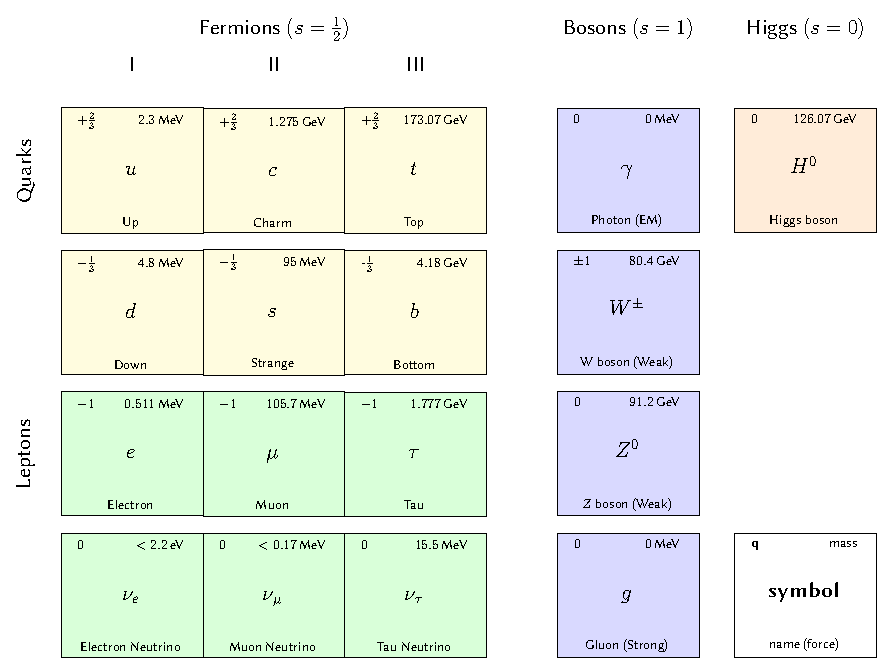
\includegraphics[width=0.95\textwidth]{PartTheory/Diagrams/ParticleTable.pdf}
    \caption[A summary of all elementary particles described by the SM]{A summary of all elementary particles described by the SM~\cite{Theory:PDGBooklet}. Note the various groupings and divisions including by spin, generation and particle type. For each particle the charge ($q$), mass and name are shown as per the legend on the bottom-right.}\label{tab:TheorySmParticles}
\end{table}

%% Table of Forces
\begin{table}[htbp]
  \centering  
    \begin{tabular}{@{}lll@{}}
      \toprule
      Name            & Relative Strength & Boson \\
      \midrule
      Strong          & \num{e38}         & Gluons \\
      Electromagnetic & \num{e36}         & Photon \\ 
      Weak            & \num{e25}         & $W$ and $Z$ \\
      Gravity         & \num{1}           & Graviton* \\
      \bottomrule
    \end{tabular}
    \caption[A summary of the four fundamental forces ordered by relative strength.]{A summary of the four fundamental forces ordered by approximated relative strength. These are included to demonstrate the large differences in strength that span many orders of magnitude. A more accurate determination of the interaction strength depends on the details of the interaction itself. $^*$ The graviton is the theoretical boson responsible for mediating gravitational interactions and is not part of the SM.}\label{tab:TheoryForces} 
\end{table}

\section{Quantum electrodynamics}

The interaction of particles via the electromagnetic force is described by \emph{quantum electrodynamics} (QED). These interactions are mediated by the massless neutral boson known as the photon and the strength of the interaction is characterized by the fine-structure constant $\alpha$. All electrically charged fermions are allowed to interact and since the photon itself is not charged, no self-interaction is allowed within QED\@. Figure~\ref{fig:TheorySimpleQED} shows the single vertex described by QED where two fermions interact via a photon. Note that the electric charge is conserved across the vertex, so for example $\gamma\rightarrow e^{+}e^{+}$ is not allowed within QED\@.

%% Simple QED Vertex
\begin{figure}[htbp]
  \centering
    \begin{fmffile}{simpleqed}
  \fmfframe(7,6)(5,4) {
    \begin{fmfgraph*}(100,80)
      \fmftop{fi,fo} \fmfbottom{Photon}
      \fmf{fermion}{fi,vx1,fo}
      \fmf{boson,label=$\gamma$}{vx1,Photon}
      \fmflabel{$f$}{fi} \fmflabel{$f$}{fo}
      \fmfdot{vx1}
    \end{fmfgraph*}
    }
\end{fmffile}
    \caption[The fundamental interaction vertex described by QED.]{The fundamental interaction vertex described by QED. The straight-lines represent any charged fermion, while the wavy line is a photon. All possible QED vertices can be obtained by simply rotating this vertex.}\label{fig:TheorySimpleQED}
\end{figure}

By combining different forms of this vertex one can build every possible QED interaction. The interaction $e^{+}e^{-}\rightarrow e^{+}e^{-}$ is known as Bhabha scattering. Two leading order (LO)\footnote{The simplest diagram with the least number of vertices} diagrams contribute to this interaction, annihilation (Figure~\ref{fig:TheoryQEDTreeA}) and scattering (Figure~\ref{fig:TheoryQEDTreeB}).

%% Example Tree Level Diagrams
\begin{figure}[htbp]
  \centering
    \begin{minipage}[][][t]{.47\textwidth}
      \centering
        \begin{fmffile}{TheoryQEDTreeA}
\fmfframe(5,17)(20,17) {
\begin{fmfgraph*}(100,80)
\fmfleft{ele1,pos1}
\fmfright{ele2,pos2}
\fmf{fermion}{ele1,v1}
\fmf{fermion}{v1,pos1}
\fmf{photon,label=$\gamma$}{v1,v2}
\fmf{fermion}{ele2,v2}
\fmf{fermion}{v2,pos2}
\fmflabel{$e^{+}$}{pos1} \fmflabel{$e^{+}$}{pos2}
\fmflabel{$e^{-}$}{ele1} \fmflabel{$e^{-}$}{ele2}
\fmfdot{v1,v2}
\end{fmfgraph*}
}
\end{fmffile}
        \subcaption{Electron-positron pair annihilation.}\label{fig:TheoryQEDTreeA}
    \end{minipage}
    \,
    \begin{minipage}[][][t]{.47\textwidth}
      \centering
        \begin{fmffile}{TheoryQEDTreeB}
\fmfframe(5,17)(20,17) {
\begin{fmfgraph*}(100,80)
\fmfleft{ele1,pos1}
\fmfright{ele2,pos2}
\fmf{fermion}{ele1,v1}
\fmf{fermion}{v1,ele2}
\fmf{photon,label=$\gamma$}{v1,v2}
\fmf{fermion}{v2,pos1}
\fmf{fermion}{pos2,v2}
\fmflabel{$e^{+}$}{pos1} \fmflabel{$e^{+}$}{pos2}
\fmflabel{$e^{-}$}{ele1} \fmflabel{$e^{-}$}{ele2}
\end{fmfgraph*}
}
\end{fmffile}
        \subcaption{Electron-positron pair scattering.}\label{fig:TheoryQEDTreeB}
    \end{minipage}
    \caption[Feynman diagrams of the process $e^{+}e^{-}\rightarrow e^{+}e^{-}$ allowed in QED at leading order.]{Feynman diagrams of the process $e^{+}e^{-}\rightarrow e^{+}e^{-}$ allowed in QED at leading order. Additional vertices can be added to produce higher-order diagrams of the same process.}\label{fig:TheoryQEDTree}
\end{figure}

\section{Quantum chromodynamics}

Interactions via the strong force are described in the theory of \emph{quantum chromodynamics} (QCD). These interactions are mediated by a set of massless neutral bosons known as gluons. QCD introduces the concept of colour which dictates which interactions are allowed via the strong force. Colour can take three states, red (anti-red), blue (anti-blue), green (anti-green):
%
\begin{equation}
  r=\begin{pmatrix}
    1 \\
    0 \\
    0 \\
  \end{pmatrix},
  \qquad
  g=\begin{pmatrix}
    0 \\
    1 \\
    0 \\
  \end{pmatrix},
  \qquad
  b=\begin{pmatrix}
    0 \\
    0 \\
    1 \\
  \end{pmatrix}
  \end{equation}

  \begin{equation}
  \bar{r}=\begin{pmatrix}
    1 &
    0 &
    0 
  \end{pmatrix},
  \qquad
  \bar{g}=\begin{pmatrix}
    0 &
    1 &
    0 
  \end{pmatrix},
  \qquad
  \bar{b}=\begin{pmatrix}
    0 &
    0 &
    1 
  \end{pmatrix}
\end{equation}

Both quarks and gluons possess colour and as a result gluons can self-interact in a three gluon vertex (Figure~\ref{fig:TheoryQCDThreeGluon}) or a four gluon vertex (Figure~\ref{fig:TheoryQCDFourGluon}). As with electrical charge, colour-charge must also be conserved. In the scattering process $q\rightarrow qg$, shown in Figure~\ref{fig:TheoryQCDColour}, the flavour of the quark does not change but the colour-charge does. The difference in colour is carried away by scattered gluon. Thus each gluon has two colour states associated with it, a colour state and an anti-colour state. Naively one would expect nine different types of gluons that participate in interaction, because of the nine combinations of colour and anti-colour. However the SU(3) symmetry on which QCD is based results in a colour octet:
%
\begin{equation}
  \begin{aligned}[c]
    &(r\bar{b}+b\bar{r})/\sqrt{2} \\
    -i&(r\bar{b}-b\bar{r})/\sqrt{2} \\
    &(r\bar{r}+b\bar{b})/\sqrt{2} \\
    &(r\bar{g}+g\bar{r})/\sqrt{2}
  \end{aligned}
  \qquad\qquad
  \begin{aligned}[c]
    -i&(r\bar{g}-g\bar{r})/\sqrt{2} \\
    &(b\bar{g}+g\bar{b})/\sqrt{2} \\
    -i&(b\bar{g}-g\bar{b})/\sqrt{2} \\
    &(r\bar{r}+b\bar{b}-2g\bar{g})/\sqrt{6}
  \end{aligned}
\end{equation}
%
and the overall colourless ``colour singlet'':
%
\begin{equation}
  (r\bar{r} + g\bar{g} + b\bar{b})/\sqrt{3}
\end{equation}

There are eight different gluons that can participate in interactions each with a different colour-charge combination, and a ninth colourless gluon that does not interact. Gluons being colour-charged has far reaching consequences for QCD\@.

In the realm of QED the vacuum around an electric charge becomes polarized as opposite charges get attracted and like charges are repelled. This has the effect of partially cancelling out the electric field experienced at a finite distance from the central charge. This effect is known as screening and also occurs with colour-charge. Quark-antiquark pairs screen the true colour-charge of the central real quark.

However, since gluons also carry colour they cause the opposite effect (anti-screening) to amplify and change the observed colour of the quark. Which effect, screening or anti-screening, wins out depends on the number of colours in the theory and the number of quark flavours. Currently, three colour states and six different quark flavours are known. This makes screening the overall dominant effect and as a result, the colour potential decreases with distance and quarks experience very little potential when very near to each other. This phenomenon is known as asymptotic freedom and forces quarks to form bound colourless states known as \emph{hadrons}.

Hadrons can be divided into two categories: \emph{mesons}, which contain a quark and an antiquark ($q\bar{q}$); and \emph{baryons}, which are made of three quarks (or antiquarks) each with a different (anti)colour-charge to result in a colourless composite particle. Common examples of baryons are protons ($uud$) and neutrons ($udd$) which are the building blocks of atomic nuclei. The pion $\pi^{0}=u\bar{u}/d\bar{d}$ is a meson which is commonly produced in hadron colliders. Due to their quark configuration, baryons have baryon number $B=+1$ while mesons have $B=0$.
  
%% Self-interacting QCD Gluon vertices
\begin{figure}[htbp]
  \centering
    \begin{minipage}[][][t]{.32\textwidth}
      \centering
      \begin{fmffile}{ColourQCD}
\begin{fmfgraph*}(100,80)
\fmftop{qin,qout} \fmfbottom{glu}
\fmf{quark}{qin,vertex1,qout}
\fmf{gluon,label=$g$,l.d=10}{vertex1,glu}
\fmfdot{vertex1}
\fmflabel{$q$}{qin} \fmflabel{$q$}{qout}
\end{fmfgraph*}
\end{fmffile}
      \subcaption{Quark-gluon vertex}\label{fig:TheoryQCDColour}
    \end{minipage}
    \begin{minipage}[][][t]{.32\textwidth}
      \centering
        \begin{fmffile}{selfqcd3}%
  \fmfframe(6,10)(1,10) {%
    \begin{fmfgraph*}(100,80)%
      \fmfleft{glu1}
      \fmfright{glu3,glu4}
      \fmf{gluon}{vertex1,glu1}
      \fmf{gluon}{glu3,vertex1} \fmf{gluon}{glu4,vertex1}
      \fmfdot{vertex1}
      \fmflabel{$g$}{glu1}
      \fmflabel{$g$}{glu3}
      \fmflabel{$g$}{glu4}
    \end{fmfgraph*}%
  }%
\end{fmffile}%
        \subcaption{Three-gluon vertex}\label{fig:TheoryQCDThreeGluon}
    \end{minipage}
    \begin{minipage}[][][t]{.32\textwidth}
      \centering
        \begin{fmffile}{selfqcd4}
\fmfframe(5,17)(20,17) {
\begin{fmfgraph*}(100,80)
\fmfleft{glu1,glu2}
\fmfright{glu3,glu4}
\fmf{gluon}{vertex1,glu1} \fmf{gluon}{vertex1,glu2}
\fmf{gluon}{glu3,vertex1} \fmf{gluon}{glu4,vertex1}
\fmfdot{vertex1}
\fmflabel{$g$}{glu1} \fmflabel{$g$}{glu2}
\fmflabel{$g$}{glu3} \fmflabel{$g$}{glu4}
\end{fmfgraph*} 
}
\end{fmffile}
        \subcaption{Four-gluon vertex}\label{fig:TheoryQCDFourGluon}
    \end{minipage}  
    \caption[The fundamental interaction vertices described by quantum chromodynamics.]{The fundamental interaction vertices described by quantum chromodynamics. Shown are \subref{fig:TheoryQCDColour} gluon emission from a quark, \subref{fig:TheoryQCDThreeGluon} gluon emission from a gluon, and \subref{fig:TheoryQCDFourGluon} the four-gluon vertex.}\label{fig:TheoryQCDVertexes}
\end{figure}

\section{Weak interactions}\label{sec:TheoryWeakInteractions}

The final type of interaction involves the so-called weak force. The weak force is responsible for common nuclear processes such as for $\beta^{-}$ decay ($n\rightarrow pe^{-}\bar{\nu}_{e}$). Interactions via the weak force are mediated by three massive bosons: the neutral $Z^{0}$ boson and the $W^{+}$ and $W^{-}$ bosons. Since these posses mass the range of interaction is very short, unlike electromagnetic interactions via a massless photon.

All fermions can interact via the weak force, but to start lets consider weak interactions involving only leptons. A valid interaction via the weak force occurs via a combination of the fundamental vertices shown in Figure~\ref{fig:TheoryWeakVertexes}, while conserving electric charge and lepton flavour. Weak bosons also couple to each other via the vertex $Z\rightarrow W^{-}W^{+}$. As the $W$ bosons have charge they also couple to the photon.

%% Weak Neutral Vertexes
\begin{figure}[htbp]
  \centering
    \begin{minipage}[][][t]{.32\textwidth}
      \centering
        \begin{fmffile}{WeakNeutral}
  \fmfframe(5,10)(6,10) { % left, top, right, bottom
    \begin{fmfgraph*}(100,80)
      \fmftop{fi,fo} \fmfbottom{ZBoson}
      \fmf{fermion}{fi,vx1,fo}
      \fmf{boson,label=$Z^{0}$}{vx1,ZBoson}
      \fmflabel{$f$}{fi} \fmflabel{$\overline{f}$}{fo}
      \fmfdot{vx1}
    \end{fmfgraph*}
  }
\end{fmffile}
        \subcaption{Neutral vertex}\label{fig:TheoryWeakNeutralFermions}
    \end{minipage}
    \begin{minipage}[][][t]{.32\textwidth}
      \centering
        \begin{fmffile}{WeakCharged}
\begin{fmfgraph*}(100,80)
\fmftop{fi,fo} \fmfbottom{WBoson}
\fmf{fermion}{fi,vx1,fo}
\fmf{boson,label=$W$}{vx1,WBoson}
\fmflabel{$\ell$}{fi} \fmflabel{$\nu_{\ell}$}{fo}
\fmfdot{vx1}
\end{fmfgraph*}
\end{fmffile}
        \subcaption{Charged vertex (leptons)}\label{fig:TheoryWeakChargedLeptons}
    \end{minipage}
    \begin{minipage}[][][t]{.32\textwidth}
      \centering
        \begin{fmffile}{WeakChargedQuark}
  \fmfframe(5,10)(6,10) {%
    \begin{fmfgraph*}(100,80)
      \fmftop{fi,fo} \fmfbottom{WBoson}
      \fmf{fermion}{fi,vx1,fo}
      \fmf{boson,label=$W$}{vx1,WBoson}
      \fmflabel{$\overline{q}$}{fi} \fmflabel{$q'$}{fo}
      \fmfdot{vx1}
    \end{fmfgraph*}
  }
\end{fmffile}
        \subcaption{Charged vertex (quarks)}\label{fig:TheoryWeakChargedQuarks}
    \end{minipage}
    \caption[The fundamental interaction vertices described by the weak theory.]{The fundamental interaction vertices described the weak theory. Shown are the \subref{fig:TheoryWeakNeutralFermions} neutral vertex, \subref{fig:TheoryWeakChargedLeptons} charged vertex with leptons, and \subref{fig:TheoryWeakChargedQuarks} charged vertex with quarks. Where $f=e\textrm{, }\mu\textrm{, }\tau$ and $\nu_{\ell}$ is the corresponding lepton neutrino of the same flavour.}\label{fig:TheoryWeakVertexes}
\end{figure}

Weak interactions involving quarks are more complicated than those with only leptons. The neutral vertex is similar to that of the leptonic version, a quark scattering off a \Z\ boson. However, the charged current changes the flavour of an up-type quark into a down-type quark (or vice-versa) with an associated \W\ boson of the appropriate charge (Figure~\ref{fig:TheoryWeakChargedQuarks}). This change in flavour can also happen across quark generations. The semileptonic decay of $b$-quarks is an example of flavour changing charged weak interactions. The $b$-quark (in a $B$ meson bound state) transitions into a $c$-quark by emitting a $W$ boson. In order to account for such an interaction and preserve the universality of weak interactions, Nicola Cabibbo postulated~\cite{Theory:CKMNicola} that the states that couple to the charged current are really a mixture of `rotated' quark states:
%
\begin{equation}
  \begin{pmatrix}
    u \\
    d' \\
  \end{pmatrix}
  \begin{pmatrix}
    c \\
    s' \\
  \end{pmatrix}
\end{equation}
%
where
%
\begin{subequations}
  \begin{equation}
  \label{eq:TheoryWeakQuarkMixingEq1}
  d'=d\cos\theta_{c} + s\sin\theta_{c}
  \end{equation}
  \begin{equation}
  \label{eq:TheoryWeakQuarkMixingEq2}
  s'=-d\sin\theta_{c} + s\cos\theta_{c}
  \end{equation}
\end{subequations}

This introduces an arbitrary parameter into the theory known as the quark mixing angle or the Cabibbo angle $\theta_{c}$. The introduction of quark mixing has the effect of attenuating the interaction strength at vertices involving multiple quark generations. Interactions which cross one generation are said to be Cabibbo Suppressed while those that cross two generations are Doubly Cabibbo suppressed.

Taking into account the three quark generations, quark mixing can be expressed in matrix notation as shown in Equation~\ref{eq:TheoryWeakQuarkMixingMatrix}. This unitary matrix is known as the Cabibbo-Kobayashi-Maskawa matrix (CKM matrix) after Cabibbo which initially postulated quark mixing, and Makoto Kobayashi and Toshihide Maskawa who later added an additional generation, containing the top and bottom quarks, to the matrix~\cite{Theory:CKMKobayashiMaskawa}. The interaction strength at a given vertex is then proportional to $|V_{ij}|^{2}$.

\begin{equation}
  \label{eq:TheoryWeakQuarkMixingMatrix}
  \begin{pmatrix}
    d' \\
    s' \\
    b' \\
  \end{pmatrix}
  =
  V_{CKM}
  \begin{pmatrix}
    d \\
    s \\
    b \\
  \end{pmatrix}
  =
  \begin{pmatrix}
    V_{ud} & V_{us} & V_{ub} \\
    V_{cd} & V_{cs} & V_{cb} \\
    V_{td} & V_{ts} & V_{tb} \\
  \end{pmatrix}
  \begin{pmatrix}
    d \\
    s \\
    b \\
  \end{pmatrix}
\end{equation}

Several parametrizations of the CKM matrix exist, the Chau-Keung parametrization~\cite{Theory:ChauKungCKM} uses angles $\theta_{\textrm{12}}$, $\theta_{\textrm{23}}$, $\theta_{\textrm{13}}$ and a phase $\delta_{\textrm{13}}$:

\begin{equation}
  \label{eq:TheoryWeakCKMStandard}
  V_{CKM}
  =
  \scalebox{0.85}{\mbox{
  \ensuremath{\displaystyle \begin{pmatrix}
    c_{12}c_{13} & s_{12}c_{13} & s_{13}\exp(-i\delta) \\
    -s_{12}c_{23}-c_{12}s_{23}s_{13}\exp(i\delta) & c_{12}c_{23} - s_{12}s_{23}s_{13}\exp(i\delta) & s_{23}c_{13} \\ 
    s_{12}s_{23}- c_{12}c_{23}s_{13}\exp(i\delta) & -c_{12}s_{23}-s_{12}c_{23}s_{13}\exp(i\delta) & c_{23}c_{13} \\
  \end{pmatrix}}
  }}
\end{equation}
%
where $c_{ij}=\cos\theta_{ij}$ and $s_{ij}=\sin\theta_{ij}$ for $i=1$,2,3. This parametrization has the advantage that each angle $\theta_{ij}$ relates to a specific transition from one generation to the other. If $\theta_{13} = \theta_{23} = 0$ the third generation is not coupled to the other two and the matrix is reduced to the one postulated by Cabibbo. Note that $\theta_{12}$ is the Cabibbo angle described earlier.

Another parametrization due to Wolfenstein~\cite{Theory:CKMWolfenstein} expresses all elements in terms of the Cabibbo angle by defining $\lambda\equiv s_{12}=\sin \theta_{12}$ and then expressing the other elements in powers of $\lambda$
%
\begin{equation}
  V_{CKM}
  \approx
  \begin{pmatrix}
  1-\lambda^2/2 & \lambda & A\lambda^3(\rho-i\eta) \\
  -\lambda & 1-\lambda^2/2 & A\lambda^2 \\ 
  A\lambda^3(1-\rho-i\eta) & -A\lambda^2 & 1\\
  \end{pmatrix}
\end{equation}
%
where $A$, $\rho$ and $\eta$ are all real numbers that express the order of magnitude differences between $s_{12}$ and the other elements in the matrix.

All the elements should be the same irrespective of which parametrization is used. The elements of the CKM matrix have been measured and the latest accepted results~\cite{Theory:PDGBooklet} are summarized in Equation~\ref{eq:TheoryWeakCKM}. 

The unitarity of the CKM matrix implies that the probability of transition from any up-type quark to any down-type is the same,
%
\begin{equation} 
  \label{eq:TheoryWeakMixingTotal}
  \sum_{k}|V_{ik}|^{2}=\sum_{i}|V_{ik}|^{2}=1
\end{equation}
%
for all $i$ quark generations~\cite{Theory:WeakUniversaility}.
The term $V_{tb}$ is approximately unity and by far dominates over the other $V_{tj}$ terms. This means that the top quark transitions almost exclusively into a $b$-quark ($t\rightarrow Wb$) with transitions $t\rightarrow Ws$ and $t\rightarrow Wd$ having a probability of less than $1\%$. The soft muon tagger which is the focus of this thesis relies on weak semileptonic decays of $b$-quarks. From~\ref{eq:TheoryWeakCKM} one can see that the transition $b\rightarrow c$ dominates over $b\rightarrow u$. This thesis concerns itself with \ttbar\ events in the lepton plus jets channel where one $W$ boson decays hadronically with a rate governed by the elements of the matrix.

\begin{equation}
  V_{CKM}
  =
  \begin{pmatrix}
    0.97427\pm0.00015 & 0.22534\pm00065 & 0.00351\;\substack{+\;0.00015\\-\;0.00014} \\
    0.22520\pm0.00065 & 0.97344\pm0.00016 & 0.0412\;\substack{+\;0.0011\\-\;0.0005} \\
    0.00867\;\substack{+\;0.00029\\-\;0.00031} & 0.0404\;\substack{+\;0.0011\\-\;0.0005} & 0.999146\;\substack{+\;0.000021\\-\;0.000046} \\
  \end{pmatrix}
  \label{eq:TheoryWeakCKM}
\end{equation}

An additional unique feature of weak interactions is that the charge conjugation-parity ($CP$) symmetry is violated. The operator $C$ denotes the change of a particle by its antiparticle partner and $P$ denotes a reversal of helicity (the projection of spin onto the momentum of a particle). A clear violation of $C$ and $P$ was observed in the radioactive decay of Cobalt-60, where the resulting electrons were preferentially emitted in the opposite direction of the nuclear spin of the Cobalt~\cite{Experimentalb}. Thus weak currents only couple to left-handed neutrinos (or right-handed anti-neutrinos) which is a violation of parity. Additionally charge symmetry is also violated since a left-handed neutrino is preferentially picked over a left-handed anti-neutrino. Finally in 1964 $CP$ violation was observed in the decay of neutral kaon~\cite{Evidence}.

Thus the probability of $\bar{a}\rightarrow \bar{b}$ is not equal to that of $a\rightarrow b$. The existence of $CP$ violation has interesting consequences for the formation of the early universe. The preferential production of matter over antimatter in $CP$ violating interactions would shift the balance in favour of matter resulting in a universe similar to our own. In terms of the Wolfenstein parametrization of the CKM matrix, if $\eta=0$ there is no $CP$ violation. This parameter has been measured to be non-zero pointing to $CP$ violation.

\subsection{Electroweak unification and the Englert-Brout-Higgs mechanism}

The unification of the electromagnetic and weak theories was first proposed by Glashow and later developed by Weinberg and Salam into the electroweak theory~\cite{Model,Theory:WeakInteractionsGlashow,Theory:WeakEMInteractions}. The theory postulates that while at low energies the two forces are to be treated separately, at higher the two can be seen as a single force. Thus the two forces are different manifestation of the same ``electroweak'' interaction. There were several stumbling blocks to the unification of the forces. Firstly, the boson which drives the electromagnetic interaction, the photon, is massless while the weak bosons are both massive. Evidence for the massive nature of these bosons has been established by experimental results from the UA1 experiment at CERN~\cite{Theory:WBosonObservationPaper}.

Thus the symmetry of the theory must be spontaneously broken in some way. A mechanism for electroweak symmetry breaking (EWSB) was postulated by Higgs, Brout, Englert and others which introduces masses to the weak bosons and posits the existence of an additional scalar (spin $S=0$) boson known as the Higgs boson.

\subsubsection{Gauge theories}

Gauge invariance is one of the underlying invariances which underpins the Standard Model. Given the so-called Dirac Lagrangian\footnote{A Lagrangian is a mathematical function that describes the underlying dynamics of a system as a function of time and space coordinates ($x^{\mu}$) and their time derivatives.}
%
\begin{equation}
  \label{eq:TheoryHiggsDiracLagrangian}
  \Lagr = i\hbar c \bar{\psi}\gamma^{\mu}\partial_{\mu}\psi -mc^2\bar{\psi}\psi
\end{equation}
%
which describes a free particle of spin-$\frac{1}{2}$ with mass $m$~\cite{Theory:IntroGriffiths}. Note that it is invariant under the transformation
%
\begin{equation}
  \psi\rightarrow e^{i\theta}\psi
\end{equation}
%
where $\theta$ is a real number, since the adjoint $\bar{\psi}\rightarrow e^{-i\theta}\bar{\psi}$ and the two terms cancel out. This is known as a \emph{(global) gauge transformation} since $\theta $ is the same at all points of space-time. A \emph{(local) gauge transformation} occurs when the phase is different for different points in space-time
%
\begin{equation}
  \psi\rightarrow e^{i\theta(x)}\psi
\end{equation}

The Dirac Lagrangian in Eq.~\ref{eq:TheoryHiggsDiracLagrangian} is not invariant under a local gauge transformation since extra terms are created by the derivative. This then implies that the underlying physics of such a theory depends on position in space-time. Thus local gauge invariance must be imposed. In the case of the Dirac Lagrangian, this is done by introducing additional terms to the Dirac Lagrangian which will cancel the extra terms introduced by the local gauge transformation. As it turns out this results in the introduction of a new massless vector field that couples to $\psi$.

The new Lagrangian then describes a spin-$\frac{1}{2}$ particle with mass $m$ that interacts with a free massless field. This new field can be identified as the electromagnetic field and the spin-$\frac{1}{2}$ particles are electrons and positrons. Thus the resulting Lagrangian describes all interactions that form part of quantum electrodynamics.

A similar procedure can be applied to the colour quark model and obtain a description of all QCD interactions. However requiring that the weak theory be a gauge theory (invariant under local gauge transformation) encounters a problem since the weak bosons are known to be massive. There must be some mechanism via which the $W^{\pm}$ and $Z^{0}$ obtain mass.

\subsubsection{The Englert-Brout-Higgs mechanism}

The Englert-Brout-Higgs (EBH) mechanism posits the existence of a complex scalar field doublet that when introduced into the electroweak Lagrangian results in the weak fields acquiring a mass term. In other words the $W^{\pm}$ and $Z^{0}$ interact with the Higgs field and obtain a mass. An additional consequence of introducing the Higgs field is the inclusion of a scalar boson particle, the so-called ``Higgs boson''. Finally, the Higgs field also couples to fermions via the Yukawa coupling generating gauge invariant mass terms for the fermions as well\footnote{For a more complete description of the mathematical procedure see~\cite{Theory:IntroGriffiths}.}. This coupling is dependent on the mass of the fermion involved, for a more massive particle the coupling is stronger. This is another reason for the top quark being an object of much study.

The SM Lagrangian in its current form including the Higgs potential is shown in Equation~\ref{eq:TheorySMLagrangian}. This expression describes all possible particle interactions that form part of the SM, of particular interest are the fermion mass term which couples the fermion field $\psi$ to the scalar Higgs field $\phi$ and the Higgs kinetic and potential terms.

\begin{align}
  \Lagr = &- \underbrace{ \frac{1}{4} W^a_{\mu\nu} W^{\mu\nu a} }_{ \text{Weak Field} }
           - \underbrace{ \frac{1}{4} B_{\mu\nu} B^{\mu\nu} }_{ \text{EM Field} }
           - \underbrace{ \frac{1}{4} G^a_{\mu\nu} G^{\mu\nu a} }_{ \text{Strong Field} } \nonumber \\
          &+ \underbrace{ \bar{\psi}\slashed{D}_{\mu}\psi}_{ \text{Fermion Kinetic} }
           + \underbrace{ \lambda\bar{\psi}\psi\phi }_{ \text{Fermion Mass} } \label{eq:TheorySMLagrangian} \\
          &+ \underbrace{ |D_{\mu}\phi^2| }_{ \text{Higgs Kinetic} }
           - \underbrace{ V(\phi) }_{ \text{Higgs Potential} } \nonumber
\end{align}

The Higgs boson, and consequently the EBH mechanism, was the last remaining piece of the SM that resisted experimental confirmation. In late 2012, the ATLAS and CMS collaborations announced~\cite{Theory:HiggsDiscoveryCMS,Theory:HiggsDiscoveryATLAS} the discovery of a Higgs-like particle with a mass around \SI{125}{\GeV}~\cite{Theory:HiggsMass}, confirming the last missing component of the SM\@. However, the remaining unexplained phenomenon have yet to be theoretically described and experimentally confirmed. Due to its large mass, the top quark is of much interest to BSM searches.

% !TEX root = ../Thesis.tex
\chapter{Top quark physics}\label{ch:TopQuark}

The third generation of quarks was first proposed by Kobayashi and Maskawa in a paper published in 1973~\cite{Theory:CKMKobayashiMaskawa} as a way to explain the $CP$ violation observed in kaon decays~\cite{Evidence}. The existence of the third generation in the quark sector was confirmed when the lighter of the two constituents, the $b$-quark, was discovered in 1977~\cite{Top:bQuarkDiscovered}. 

Due to its large mass, direct production of the top quark required the construction of very powerful accelerators. However, its mass was constrained in precision electroweak measurements at LEP in 1995 to be~\cite{Top:TopMassLEP}:
%
\begin{equation}
  m_{\textrm{top}}=\num{174}\;^{+\;21.5}_{-\;25.5}\;\si{GeV}
\end{equation}

The top quark was then discovered by the CDF and D0 experiments at Fermilab in 1995~\cite{Top:ObservationCDF,Top:ObservationD0} and then observed at CERN again in 2010~\cite{TopQuark:FirstTopAtATLAS,TopQuark:FirstTopAtCMS}.

The large mass of the top quark makes it a very interesting object of study. The current world average for the mass of the top quark, based on results from Tevatron and the LHC~\cite{Theory:PDGBooklet}, is
%
\begin{equation*}
  m_{t}=173.07\pm0.52\stat\pm0.72\syst\si{\GeV}
\end{equation*}

Due to its mass the top quark has an extremely short lifetime $\tau\approx\SI{0.5e-24}{\second}$, too short to interact via the strong force and hadronize into a bound state~\cite{Theory:TopQuarkDecayTooQuickly}. Instead the top quark decays weakly producing a $W$ boson and a $b$-quark almost exclusively. This allows experimentalists to directly study the properties of a bare quark. An impossibility with the other quarks which bind with other quarks to form hadrons. Measurement of top quark properties (mass, charge, forward-backward asymmetry, couplings, etc\ldots) forms a large part of high energy physics research. Measurement of these properties provide rigorous tests of the SM, and could point towards the existence of new physics or exclude some BSM theories.

From an experimental perspective, top quark decays produce a very interesting signature with leptons, jets and missing energy due to the escaping neutrino\footnote{Neutrinos do not interact with the detector material and thus escape without being detected, missing energy is described in more detail in Chapter~\ref{ch:Detector}}. Therefore, the study of top quark decays relies on all parts of a general purpose detector such as ATLAS or CMS\@. Finally, \ttbar\ pair production also is a major background for many other SM and BSM searches, so understanding this process well is fundamental to almost all areas of HEP research.

\section{Top quark production}\label{sec:top_quark_production}

Top quarks can be produced in two ways: single top production and \ttbar\ pair production. In the SM the dominant top quark pair production mechanism proceeds via the strong force. The production cross section of $pp\rightarrow\ttbar$ depends on the mass of the top $m_{t}$, the centre of mass energy $\sqrt{s}=2E_{\textrm{beam}}$ and the fraction of the momentum taken by the partons\footnote{The constituents of hadrons: quarks and gluons} of the colliding protons.

In order to produce a \ttbar\ pair the total energy carried by the interacting partons must be larger than twice the mass of the top. Let us define the effective centre of mass energy $\hat{s}$ which reflects the true amount of energy available for interaction. Given two colliding partons, denoted $i$ and $j$ carrying $x_i$ and $x_j$ fractions of the centre of mass energy $\cme$, then
%
\begin{equation}
  \hat{s} = x_{i}\cme x_{j}\cme = x_{i}x_{j}s
\end{equation}
%
assuming that both partons carry the same fraction of the total energy, i.e. $x_i\approx x_j$ then the minimum value of $x$ required for \ttbar\ production is
%
\begin{equation}
  x\approx\frac{2m_t}{\sqrt{s}}  
\end{equation}

At the LHC the minimum threshold at $\cme=\SI{7}{\TeV}(\SI{14}{\TeV})$ is approximately 0.05(0.025). At such low values of $x$ the fraction of proton momentum carried by the gluons is large~\cite{TopQuark:HATHORCrossSection} and thus gluon fusion interactions dominate as can be seen in Figure~\ref{fig:TopMSTWNLOPDFs}.

\begin{figure}[htbp]
  \centering
    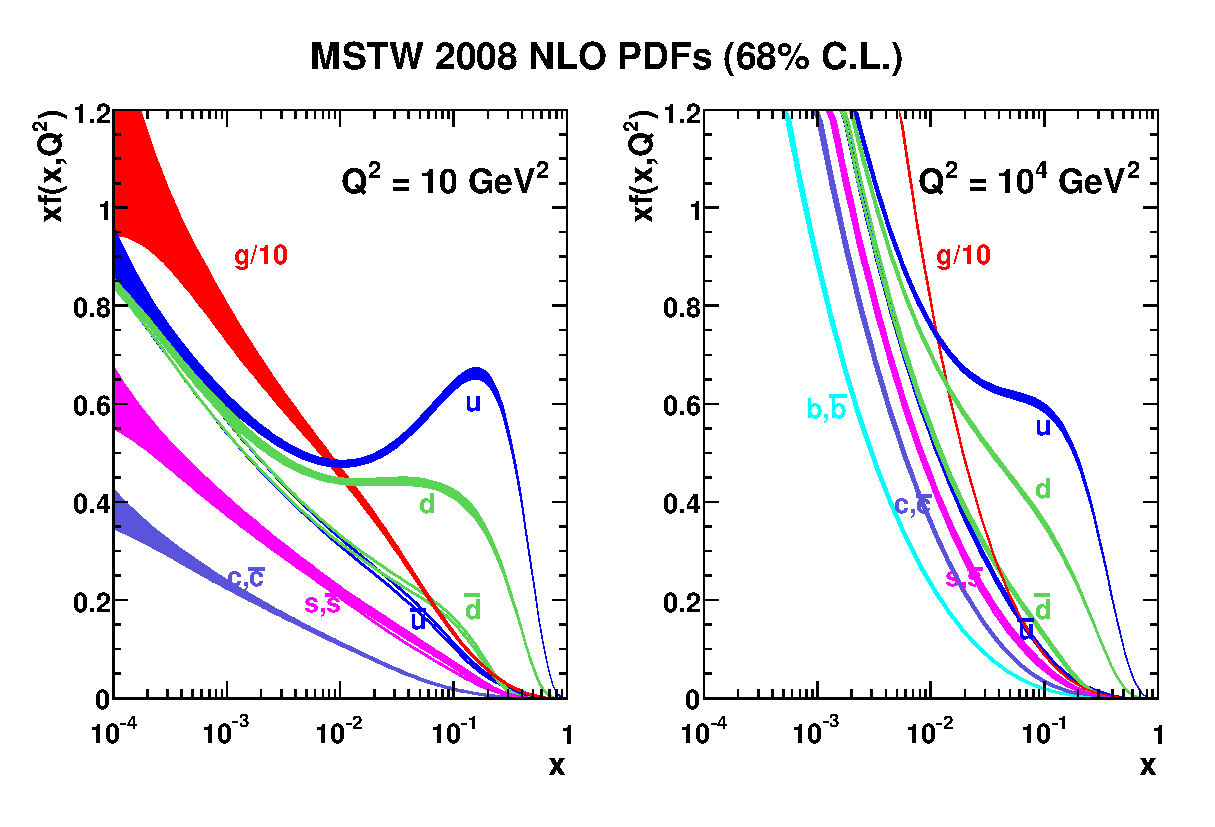
\includegraphics[width=0.75\textwidth]{PartTopQuark/Plots/mstw2008nlo68cl_allpdfs.eps}
    \caption{MSTW 2008 NLO parton distribution functions.}\label{fig:TopMSTWNLOPDFs}
\end{figure}

Gluon fusion processes represent $\num{80}(\num{90})\si{\percent}$ of the total cross section, with the remainder contribution coming from quark pair annihilation. The Feynman diagrams for these interactions are shown in Figure~\ref{fig:TopQuarkProduction}. The theoretical inclusive \ttbar\ production cross sections at the LHC has been calculated to NNLO~\cite{TopPair,TopQuark:CrossSection8TeV}:
\begin{align*}
  \cmsS\textrm{: }\sigma_{t\bar{t}} &= 158\;^{-\;12.2}_{+\;13.5}\;\si{\pico\barn} \\
  \cmsE\textrm{: }\sigma_{t\bar{t}} &= 252.9\;^{+\;6.4}_{-\;8.6}\pm11.7\;\si{\pico\barn}
\end{align*}

\begin{figure}[htbp]
  \centering
  \begin{minipage}[][][t]{.47\textwidth}
    \centering
    % !TEX root = ../../Thesis.tex
\begin{fmffile}{TopProdStraightgg2tt}
\fmfframe(5,17)(5,17) {
\begin{fmfgraph*}(150,70)
\fmfleft{gluon1,gluon2}
\fmfright{tbar,top}
\fmf{gluon}{v1,gluon1}
\fmf{gluon}{v2,gluon2}
\fmf{fermion}{tbar,v1}
\fmf{fermion,label=$t$,tension=0}{v1,v2}
\fmf{fermion}{v2,top}
\fmflabel{$g$}{gluon1} \fmflabel{$t$}{top}
\fmflabel{$g$}{gluon2} \fmflabel{$\bar{t}$}{tbar}
\end{fmfgraph*}
}
\end{fmffile}
    \subcaption{Gluon fusion (t-channel)}
  \end{minipage}
  \,
  \begin{minipage}[][][t]{.47\textwidth}
    \centering
    % !TEX root = ../../Thesis.tex
\begin{fmffile}{TopProdCrossGG2ttbar}
\fmfframe(5,17)(5,17) {
\begin{fmfgraph*}(150,70)
\fmfleft{i1,i2}
\fmfright{o1,o2}
\fmf{gluon}{v1,i1}
\fmf{phantom}{v1,o1} % Invisible rubber band
\fmf{gluon}{v2,i2}
\fmf{phantom}{v2,o2} % also invisible rubber band
\fmf{fermion,tension=0.5}{v1,v2}
% These are visible, but have no tension.
\fmf{fermion,tension=0}{o2,v1}
\fmf{fermion,tension=0}{v2,o1}
\fmflabel{$g$}{i1}
\fmflabel{$g$}{i2}
\fmflabel{$t$}{o1}
\fmflabel{$\bar{t}$}{o2}
\end{fmfgraph*}
}
\end{fmffile}
    \subcaption{Gluon fusion (u-channel)}
  \end{minipage}
  
  \begin{minipage}[][][t]{.47\textwidth}
    \centering
    % !TEX root = ../../Thesis.tex
\begin{fmffile}{TopProdgg2g2ttbar}
\fmfframe(5,17)(20,17) {
\begin{fmfgraph*}(150,70)
\fmfleft{gluon1,gluon2}
\fmfright{top1,top2}
\fmf{gluon}{v1,gluon1}
\fmf{gluon}{v1,gluon2}
\fmf{gluon,label=$g$,l.d=10}{v2,v1}
\fmf{fermion}{top1,v2,top2}
\fmflabel{$g$}{gluon1} \fmflabel{$t$}{top2}
\fmflabel{$g$}{gluon2} \fmflabel{$\bar{t}$}{top1}
\end{fmfgraph*}
}
\end{fmffile}
    \subcaption{Gluon fusion (s-channel)}
  \end{minipage}
  \,
  \begin{minipage}[][][t]{.47\textwidth}
    \centering
    % !TEX root = ../../Thesis.tex
\begin{fmffile}{TopProdqq2ttbar}
\fmfframe(5,17)(5,17) {
\begin{fmfgraph*}(150,70)
\fmfleft{q,qbar}
\fmfright{tbar,top}
\fmf{fermion}{qbar,v1,q}
\fmf{gluon,label=$g$,l.d=10}{v2,v1}
\fmf{fermion}{tbar,v2,top}
\fmflabel{$q$}{q} \fmflabel{$t$}{top}
\fmflabel{$\bar{q}$}{qbar} \fmflabel{$\bar{t}$}{tbar}
\end{fmfgraph*}
}
\end{fmffile}
    \subcaption{Quark pair annihilation}
  \end{minipage}
  \,
  \caption{The leading order Feynman diagrams for \ttbar\ production.}\label{fig:TopQuarkProduction}
\end{figure}

Single top production occurs via the weak force almost exclusively through the $Wtb$ vertex since $|V_{tb}|\gg|V_{ts}|,|V_{td}|$. At LO there are several production mechanisms for single-top events:

\begin{itemize}
  \item Weak quark-antiquark annihilation forming a \W\ which subsequently decays into a $t\bar{b}$ (Figure~\ref{fig:TopSingleSChannel}).
  \item The so-called $tW$ production, where a $b$-quark absorbs a gluon and decays to a top quark and $W$ boson (Figure~\ref{fig:TopSingletWChannel}).
  \item $b$-quark scattering off a $W$ boson, where the $b$ comes from gluon splitting (Figure~\ref{fig:TopSingleqtbChannel}) or from the proton (Figure~\ref{fig:TopSingleqtChannel}).
\end{itemize}

The cross sections for $pp\rightarrow t+X$ at the LHC have been estimated at NLO, for the t-channel~\cite{Kidonakis:2012rm}:
%
\begin{align*}
  \cmsS\textrm{: }\sigma^{\textrm{t-chan}}_{t} = \SI[multi-part-units=single]{66(2)}{\pico\barn} \\
  \cmsE\textrm{: }\sigma^{\textrm{t-chan}}_{t} = \SI[multi-part-units=single]{87(3)}{\pico\barn}
\end{align*}
%
, and for $tW$ production~\cite{TopQuark:WtOne,TopQuark:WtTwo,TopQuark:WtThree,TopQuark:WtFour}:
%
\begin{align*}
  \cmsS\textrm{: }\sigma_{tW} &= \SI[multi-part-units=single]{15.6(12)}{\pico\barn} \\
  \cmsE\textrm{: }\sigma_{tW} &= \SI[multi-part-units=single]{22.2(15)}{\pico\barn}
\end{align*}

\begin{figure}[htpb]
  \centering
  \begin{minipage}[][][t]{.47\textwidth}
    \centering
    % !TEX root = ../../Thesis.tex
\begin{fmffile}{TopSingleTopSChannel}
\fmfframe(5,17)(20,17) {
\begin{fmfgraph*}(150,70)
\fmfleft{quark,antiquark}
\fmfright{top,bbar}
\fmf{fermion}{quark,v1,antiquark}
\fmf{boson,label=$W$}{v1,v2}
\fmf{fermion}{bbar,v2,top}
\fmflabel{$q$}{quark} \fmflabel{$t$}{top}
\fmflabel{$\overline{q}'$}{antiquark} \fmflabel{$\overline{b}$}{bbar}
\fmfdot{v1,v2}
\end{fmfgraph*}
}
\end{fmffile}
    \subcaption{s-channel}\label{fig:TopSingleSChannel}
  \end{minipage}
  \,
  \begin{minipage}[][][t]{.47\textwidth}
    \centering
    % !TEX root = ../../Thesis.tex
\begin{fmffile}{TopSingleTWChannel}
\fmfframe(5,17)(20,17) {
\begin{fmfgraph*}(150,70)
\fmfleft{gluon,b}
\fmfright{top,W}
\fmf{gluon}{gluon,v1}
\fmf{fermion}{b,v1}
\fmf{fermion,label=$b$}{v1,v2}
\fmf{fermion}{v2,top}
\fmf{boson}{v2,W}
\fmflabel{$g$}{gluon} \fmflabel{$t$}{top}
\fmflabel{$b$}{b} \fmflabel{$W$}{W}
\end{fmfgraph*}
}
\end{fmffile}
    \subcaption{$tW$-channel}\label{fig:TopSingletWChannel}
  \end{minipage}

  \begin{minipage}[][][t]{.47\textwidth}
    \centering
    % !TEX root = ../../Thesis.tex
\begin{fmffile}{TopSingleQtb}
\fmfframe(5,17)(20,17) {
\begin{fmfgraph*}(150,70)
\fmfleft{glu1,quark}
\fmfright{bbar,top,qprime}
\fmf{fermion}{quark,v1,qprime}
\fmf{gluon}{glu1,v3}
\fmf{fermion}{bbar,v3}
\fmffreeze
\fmf{phantom}{v1,v3}
\fmf{boson,label=$W$}{v1,v2}
\fmf{fermion,label=$b$}{v3,v2}
\fmffreeze
\fmf{fermion}{v2,top}
\fmflabel{$g$}{glu1} \fmflabel{$t$}{top}
\fmflabel{$q$}{quark} \fmflabel{$q'$}{qprime} \fmflabel{$\bar{b}$}{bbar}
\end{fmfgraph*}
}
\end{fmffile}
    \subcaption{Associated with a $q$ and $\bar{b}$}\label{fig:TopSingleqtbChannel}
  \end{minipage}
  \,
  \begin{minipage}[][][t]{.47\textwidth}
    \centering
    % !TEX root = ../../Thesis.tex
\begin{fmffile}{TopSingleqb2qt}
\fmfframe(5,17)(20,17) {
\begin{fmfgraph*}(150,70)
\fmfleft{ib,iq}
\fmfright{ot,oq}
\fmf{fermion}{iq,v1,oq}
\fmf{fermion}{ib,v2,ot}
\fmffreeze
\fmf{boson,label=$W$}{v1,v2}
\fmflabel{$b$}{ib} \fmflabel{$t$}{ot}
\fmflabel{$q$}{iq} \fmflabel{$q'$}{oq}
\end{fmfgraph*}
}
\end{fmffile}
    \subcaption{Associated with a $q$}\label{fig:TopSingleqtChannel}
  \end{minipage}
  \caption{Example Feynman diagrams for single top quark at leading order.}\label{fig:TopSingleProduction}
\end{figure}

As top quark pair production can proceed via the strong force it occurs overwhelmingly more often than single top production. The production cross section of \ttbar\ is approximately two times larger than the single-top cross section.

\section{Top quark decay modes}\label{sec:top_quark_decay_modes}

The top quark decays almost exclusively into a $W$ boson and a $b$-quark. The world average measured ratio of branching ratios $\Gamma(t\rightarrow Wb)/\Gamma(t\rightarrow Wq(q=b,s,d))$ is \num{0.91(4)}~\cite{Theory:PDGBooklet}. Note that there is some tension between this measured result and the naive expectation from the CKM matrix. The measured value is $2\sigma$ away from the expected CKM result, meaning there is perhaps some room for additional quark generations not accounted for by the CKM matrix.

As the LHC collides proton-proton beams, the overwhelming majority of events produced will feature multiple hadronic \textit{jets}, a stream of particles resulting from the hadronization of quarks in the detector, most of which will originate from ``light'' quarks\footnote{The term light quarks usually refers to quarks in the first two generations. Light jets are those originating from those quarks}. Unlike light hadrons, $B$-hadrons have a sufficiently large lifetime that they travel a certain distance before decaying. Additional features such as the semileptonic decay of $b$-quarks can be exploited to determine the presence of such a quark in the detector. Collectively analysis techniques that permit the detection of $b$-jets are known as \textit{b-tagging}. Top quark pairs will produce two $b$-quarks, making $b$-tagging techniques a central part of any \ttbar\ analysis. More information on $b$-tagging techniques, including the Soft Muon Tagger, is provided in Chapter~\ref{ch:Detector}.

The other part of the top decay, the $W$ boson, is used to classify \ttbar\ events. The $W$ boson can decay leptonically ($W\rightarrow\ell\nu_{\ell}$) or hadronically ($W\rightarrow q\bar{q}'$) driven by the CKM vertex element. The branching ratios of $W$ boson decays are presented in Table~\ref{tab:TopQuakWDecayBranchingRatios}.

\begin{table}[htbp]
  \centering
  \begin{tabular}{@{}cS[table-format=2.2(2)]@{}}
    \toprule
    $W$ decay to & {Branching ratio [\si{\percent}]} \\
    \midrule
    $e+\nu$      & 10.75(13) \\
    $\mu+\nu$    & 10.57(15) \\
    $\tau+\nu$   & 11.25(20) \\
    Hadrons      & 67.60(27) \\
    \bottomrule
  \end{tabular}
  \caption[Branching ratios of $W$ boson decay.]{Branching ratios of $W$ boson decay. \textbf{Hadrons} refers to all possible combinations of $q\bar{q}'$ where $\bar{q}'$ denotes the antiquark of a flavour different to that of the first quark~\cite{Theory:PDGBooklet}.}\label{tab:TopQuakWDecayBranchingRatios}
\end{table}

Top quark pair events are labelled as ``dilepton'', ``all-hadronic'' or ``lepton plus jets'' depending on the combination of $W$ boson decays present. The probability for a \ttbar\ event to be of a given type is dependent on the branching ratios of $W$ boson decays shown previously. As can be seen from Figure~\ref{fig:TopQuarkDecayModes} the all-hadronic events dominate, followed by the lepton plus jets and dilepton. Each event type requires a different analysis approach due to their distinct backgrounds, branching ratio, detector signature and reconstruction requirements. Note that some lepton plus jets analyses do not explicitly treat taus directly. Nevertheless tau decays enter into these analysis via its decay to an electron or muon. Thus the true branching ratio is marginally smaller than that shown in the Figure~\ref{fig:TopQuarkDecayModes}.

\begin{figure}[tbhp]
  \centering
  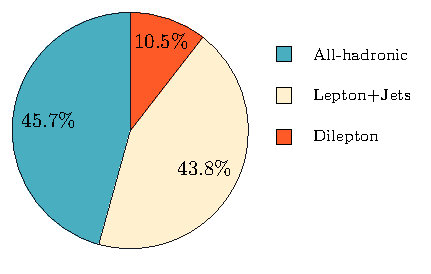
\includegraphics[width=0.75\textwidth]{PartTopQuark/Diagrams/TopQuarkDecayPie.pdf}
  \caption[Branching ratios of all possible \ttbar\ decays.]{Branching ratios of all possible \ttbar\ decays. These probabilities are based on the branching ratios of $W$ boson decay shown in Table~\ref{tab:TopQuakWDecayBranchingRatios}. Note that the lepton plus jets branching ratio here includes all three leptons.}\label{fig:TopQuarkDecayModes}
\end{figure}

The all-hadronic final state includes four light quarks which will hadronize to form four light flavour (LF) jets and two $b$-quarks leading to two $b$-jets. Due to the large hadronic activity the all-hadronic channel is very challenging. As mentioned before, hadronic collisions produce events with a large number of jets in the final state. The background to the all-hadronic channel are therefore very high. As shown in Figure~\ref{fig:TopQuarkDecayModes} the all-hadronic channel has the largest branching ratio of the three.

The dilepton final state includes two leptons, large missing energy from two neutrinos which escape the detector and two $b$-jets. In contrast to the all-hadronic channel, dilepton events are very clean due to the presence of leptons and missing energy, however the branching ratio is very small and reconstruction of the top quarks is challenging due to the presence of the two neutrinos. Finally, the lepton plus jets channel has a larger branching ratio than the dilepton while having a distinct signature with a lepton and missing energy as well as LF jets and $b$-jets.

Lepton plus jets analyses do have some acceptance to $\tau$ events, but they are not usually treated as the signal lepton. The $\tau$ lepton is unstable and decays primarily via the weak force producing hadrons in the final state. Events with $\tau$ leptons enter lepton plus jets analyses when the $\tau$ decays leptonically into a muon or electron. The reconstruction of $\tau$ leptons is a complex task and $\tau$ plus jet events are treated separately with dedicated analyses. An example of the full lepton plus jets chain is shown in Figure~\ref{fig:TopQuarkFullLPlusJets}.

\begin{figure}[p]
  \centering
  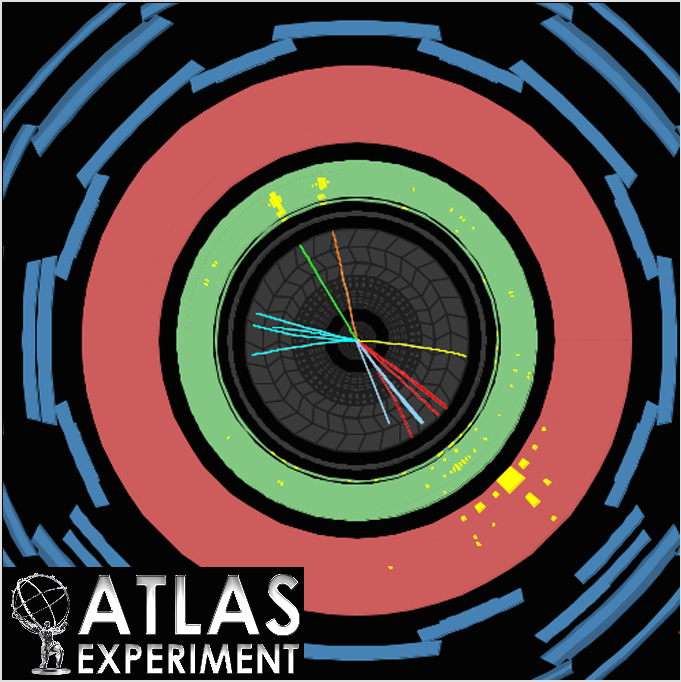
\includegraphics[height=0.65\textheight]{PartTopQuark/Diagrams/atlas-2010-063-fig_09.png}
  \caption{Example event display of a dilepton \ttbar\ event recorded by ATLAS\@. The electrons are shown as yellow energy depositions in the green EM calorimeter. These are associated with a green and orange upward-pointing tracks in the ID\@. Some hadronic activity is noted in the red hadronic calorimeter on the opposite side.}\label{fig:TopQuarkEventDisplay}
\end{figure}

The lepton plus jets channel has the advantage of a more distinct signature than the all-hadronic event as well as a suffering from less background. The branching ratio of lepton plus jets event is also approximately twice that of the dilepton channel. As a result the lepton plus jets channel has been chosen as the focus of this thesis.

\begin{figure}[htbp]
  \centering
  \begin{minipage}[][][t]{.60\textwidth}
  % !TEX root = ../../Thesis.tex
\begin{fmffile}{TopQuarkLeptonPlusJetsFull}
  \fmfframe(5,17)(20,17){
    \begin{fmfgraph*}(200,200)
      \fmfstraight
      % Input Particles
      \fmfleft{dummy1,gluon1,gluon2,dummy2}
      % Output Particles
      \fmfright{q,antiq,b,antib,lep,nu}
      % Process
      % Gluon Fusion
      \fmf{gluon}{v1,gluon1} \fmf{gluon}{v1,gluon2} \fmf{gluon,label=$g$,l.d=10}{v2,v1}
      % Top Pair Production
      \fmf{fermion,label=$t$,l.d=-14,tension=0.5}{top,v2} \fmf{fermion,label=$\bar{t}$,tension=0.5}{v2,antitop}
      % Leptonic Side
      \fmf{fermion,tension=0,tension=0}{antib,antitop}
      \fmf{boson,label=$W$,tension=0}{antitop,leptonicW}
      \fmf{fermion}{nu,leptonicW,lep}
      % Hadronic Side
      \fmf{fermion,tension=0}{b,top}
      \fmf{boson,label=$W$,tension=0}{hadronicW,top}
      \fmf{fermion,tension=0}{antiq,hadronicW,q}
      % Labels
      % In
      \fmflabel{$g$}{gluon1} \fmflabel{$g$}{gluon2}
      % Out
      % Hadronic Side
      \fmflabel{$b$}{b} \fmflabel{$\bar{q}'$}{q} \fmflabel{$q$}{antiq}
      % Leptonic Side
      \fmflabel{$\bar{b}$}{antib} \fmflabel{$\ell$}{lep} \fmflabel{$\nu_{\ell}$}{nu}
    \end{fmfgraph*}
  }
\end{fmffile}
  \end{minipage}
  \caption[Feynman diagram of lepton plus jets channel including \ttbar\ production via gluon fusion and decay with a leptonically decaying $W^{+}$.]{Feynman diagram of lepton plus jets channel including \ttbar\ production via gluon fusion and decay with a leptonically decaying $W^{+}$. All other production mechanisms are also considered and the final state where the $W^{-}$ decays leptonically is also taken into account.}\label{fig:TopQuarkFullLPlusJets}
\end{figure}

\section{Latest developments in top physics}

This section discusses a few of the latest measurements in the area of top quark pair production with a focus on LHC results. Top quark decays provide the only probe to study the properties of a bare quark. Measurements of its properties provide a stringent test of the SM and could show hints of new physics from BSM theories. Moreover, due to its final state signature top quark pair production, particularly in the lepton plus jets channel, form the background to many searches for new physics.  All parts of the detector are utilized in the reconstruction of $\ell$+jets events and so it is possible to use these events to tune or \textit{calibrate} analysis and reconstruction techniques.

\subsubsection{Cross section measurement}

Measurement of the production cross section of the top quark at different centre of mass energies\footnote{The production cross section is dependent on the centre of mass energy of the collision.} is a benchmark test of the SM. Any statistically significant deviation from the predicted value could point to the presence of new physics. Some BSM theories posit the existence of particles which could decay to produce a \ttbar\ pair. If such theory is correct this would be observed in an increase in the cross section measured away from the predicted SM value. Precise knowledge of the cross section is also vital from an experimental perspective, for example when attempting to reduce and estimate the amount of top quark background present in other analyses. Searches for the Higgs boson exploit many different channels such as $t\bar{t}H\rightarrow t\bar{t}b\bar{b}$ which have \ttbar\ events as a background. The type of events predicted by the BSM theory, supersymmetry (SUSY) include a large amount of missing energy, leptons and jets in the final state. Top quark pair events mimic these processes and constitute a large background.

A summary of all \ttbar\ cross section measurements from the LHC at \cmsS\ is shown in Figure~\ref{fig:TopQuarkPairProductionSummaryLHC} and a comparison against the Tevatron measurement at $\sqrt{s}=\SI{1.96}{\TeV}$ is shown in Figure~\ref{fig:TopQuarkPairProductionComparison}. Early results at \cmsE\ are shown in Figure~\ref{fig:TopQuarkPairProduction8TeV}.

\begin{figure}[htbp]
  \centering
  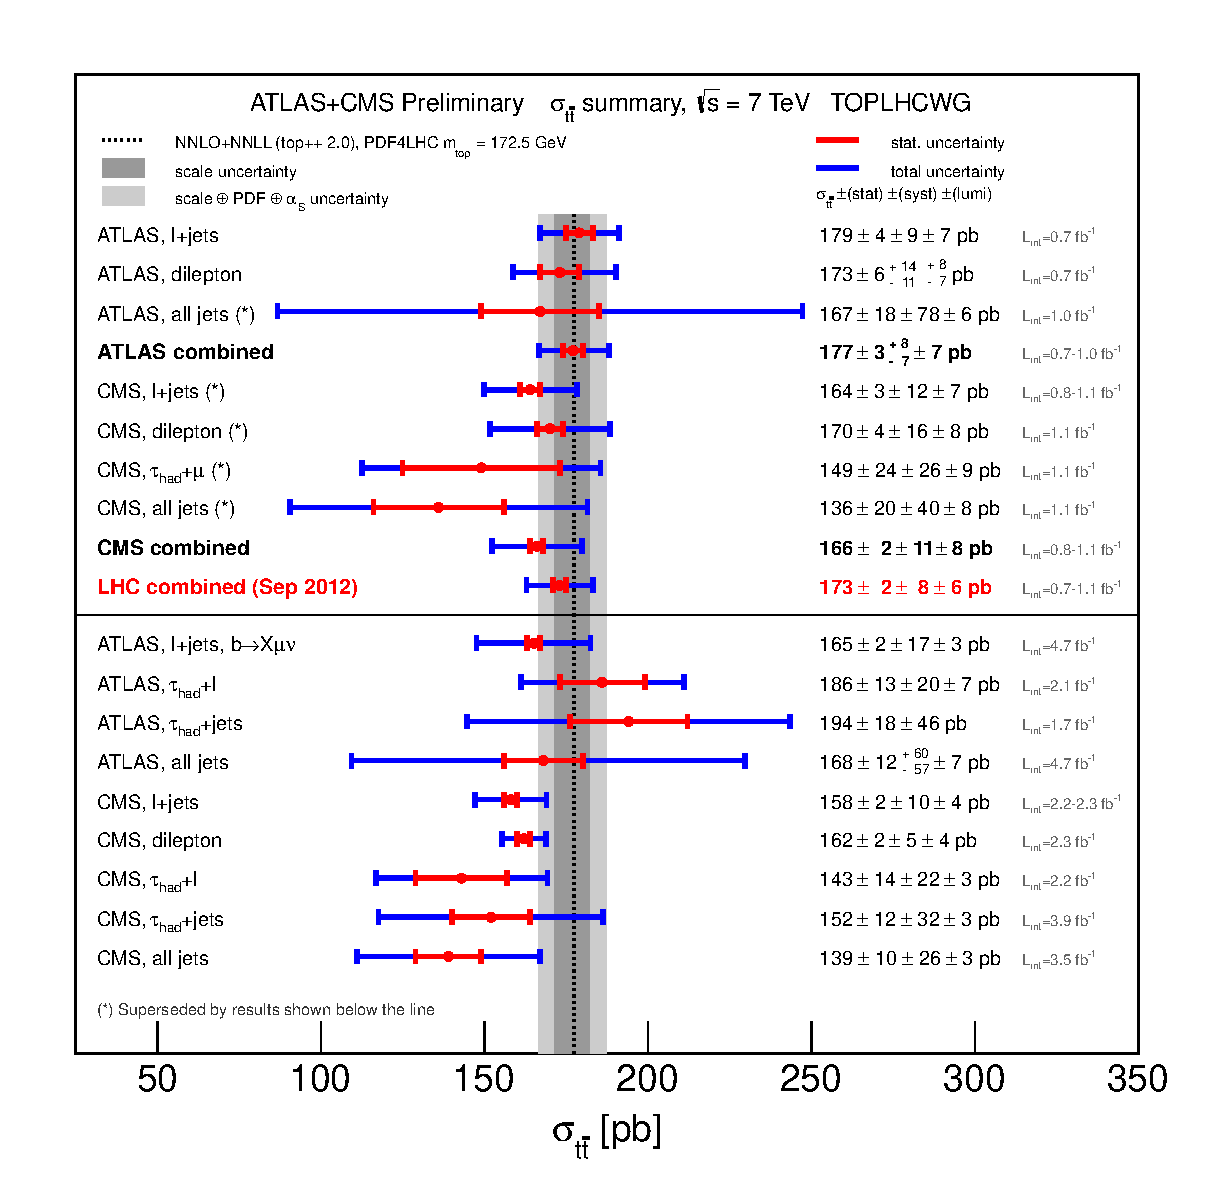
\includegraphics[width=0.75\textwidth]{PartTopQuark/Plots/tt_xsec_7TeV.eps}
  \caption[A summary of all \ttbar\ production cross section measurements performed at the LHC at \cmsS.]{A summary of all \ttbar\ production cross section measurements performed at the LHC at \cmsS~\cite{TopQuark:SummaryPlots}. The theory prediction shown as a dotted black line associated uncertainties as grey bands. The results shown above the black line have been statistically combined, producing the results labelled as \textbf{combined}. Many of these analyses have been superseded and the results are shown below the line. Other analyses performed but not included in the combination are also shown below the line, such as the analysis described in Chapter~\ref{ch:CrossSection}.}\label{fig:TopQuarkPairProductionSummaryLHC}
\end{figure}

\begin{figure}[htbp]
  \centering
  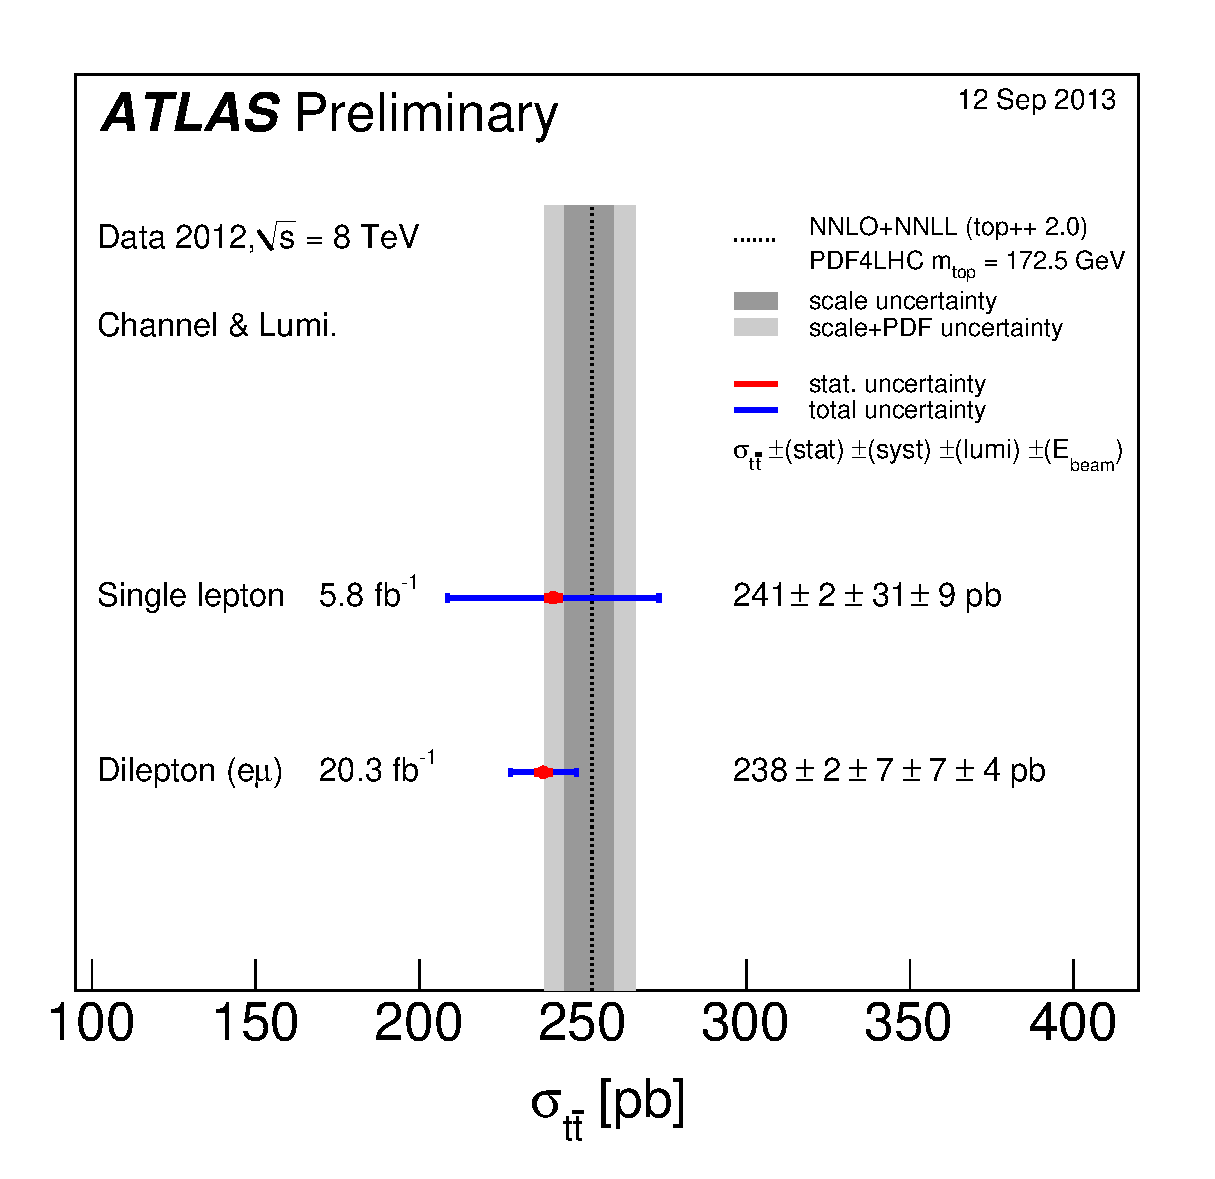
\includegraphics[width=0.75\textwidth]{PartTopQuark/Plots/tt_xsec_8TeV.eps}
  \caption[A summary of all \ttbar\ production cross section measurements performed at the LHC at \cmsE.]{A summary of all \ttbar\ production cross section measurements performed at the LHC at \cmsE~\cite{TopQuark:SummaryPlots}. The theory prediction is shown as a dotted line with associated uncertainties as grey bands.}\label{fig:TopQuarkPairProduction8TeV}
\end{figure}

\begin{figure}[htbp]
  \centering
  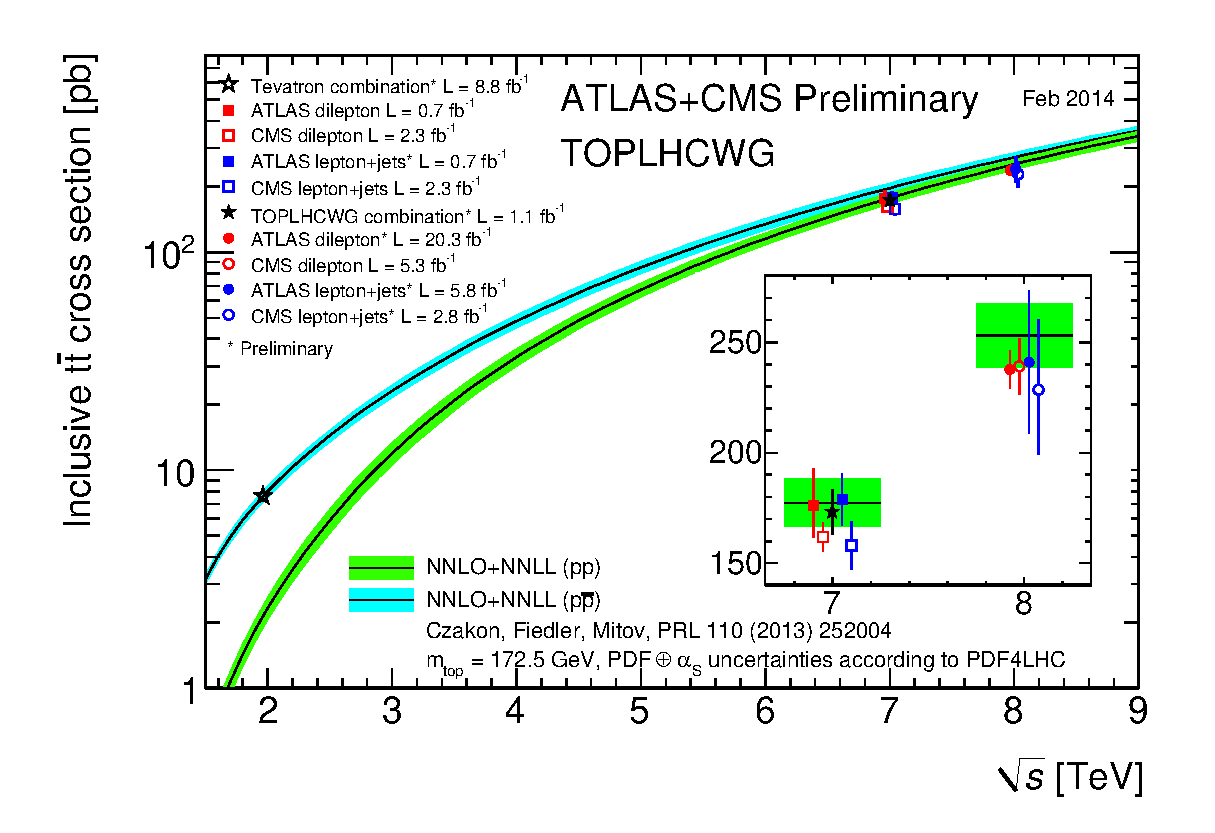
\includegraphics[width=0.75\textwidth]{PartTopQuark/Plots/tt_xsec_vsroots.eps}
  \caption[A summary of the most precise \ttbar\ production cross section measurements performed at the LHC at $\sqrt{s}=$ 7 and 8 TeV and the Tevatron at $\sqrt{s}=\SI{1.96}{\TeV}$ compared to the theoretical prediction.]{A summary of the most precise \ttbar\ production cross section measurements performed at the LHC at $\sqrt{s}=$ 7 and 8 TeV and the Tevatron at $\sqrt{s}=\SI{1.96}{\TeV}$ compared to the theoretical prediction~\cite{TopQuark:SummaryPlots}. The Tevatron results should be compared against the prediction for $p\bar{p}$ collisions while the LHC against the $pp$ collision predictions.}\label{fig:TopQuarkPairProductionComparison}
\end{figure}

\subsubsection{Top mass measurement}

The mass of the top $m_{t}$ is a fundamental parameter of the SM\@. Measurements of the top mass have been carried out in all \ttbar\ channels at both ATLAS and CMS~\cite{Top:TopMassCombination}. These results are summarized in Figure~\ref{fig:TopQuarkMtopSummaryATLAS}, which includes the combined LHC measurement:
%
\begin{equation*}
  m_{t}=173.29\pm0.23\stat\pm0.92\syst\si{\GeV}
\end{equation*}

\begin{figure}[htbp]
  \centering
  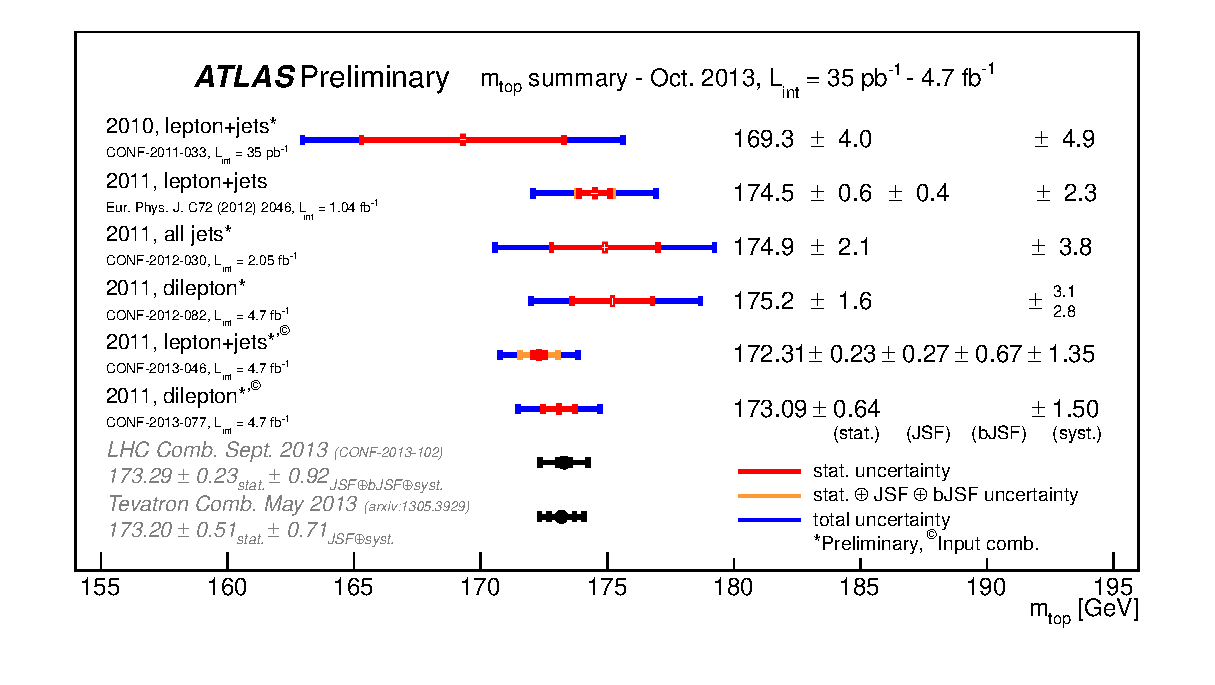
\includegraphics[width=0.75\textwidth]{PartTopQuark/Plots/mtopHistory_ATLASAll.eps}
  \caption[Summary of all $m_{t}$ measurement results per analysis at ATLAS.]{Summary of all $m_{t}$ measurement results per analysis at ATLAS~\cite{TopQuark:SummaryPlots}. The statistical combination of these results are compared to the combination from Tevatron.}\label{fig:TopQuarkMtopSummaryATLAS}
\end{figure}

\subsubsection{Boosted top resonance searches}

Some BSM theories predict the existence of additional particles with large masses that can decay into a pair of top quarks with very large transverse momenta. The decay products of these highly boosted tops emerge in a collimated cone. Boosted top searches have been carried out at ATLAS~\cite{Boosted:ATLASExclusion7TeV}, looking for the decay products of a heavy boson known as the $Z'$~\cite{TopQuark:TC2,TopQuark:TC22,TopQuark:ZPrimeCross} and Kaluza-Klein gluons~\cite{TopQuark:KKGluonTwo,TopQuark:KKGluonOne,TopQuark:KKGluonThree,TopQuark:KKGluonFour,TopQuark:KKGluonFive}. A narrow leptophobic $Z'$ with a mass of less than \SI{1.74}{\TeV} is excluded and a Kaluza-Klein gluon is excluded for masses below \SI{2.07}{\TeV} as shown in Figure~\ref{fig:BoostedLimits}.

\begin{figure}[htbp]
  \centering
  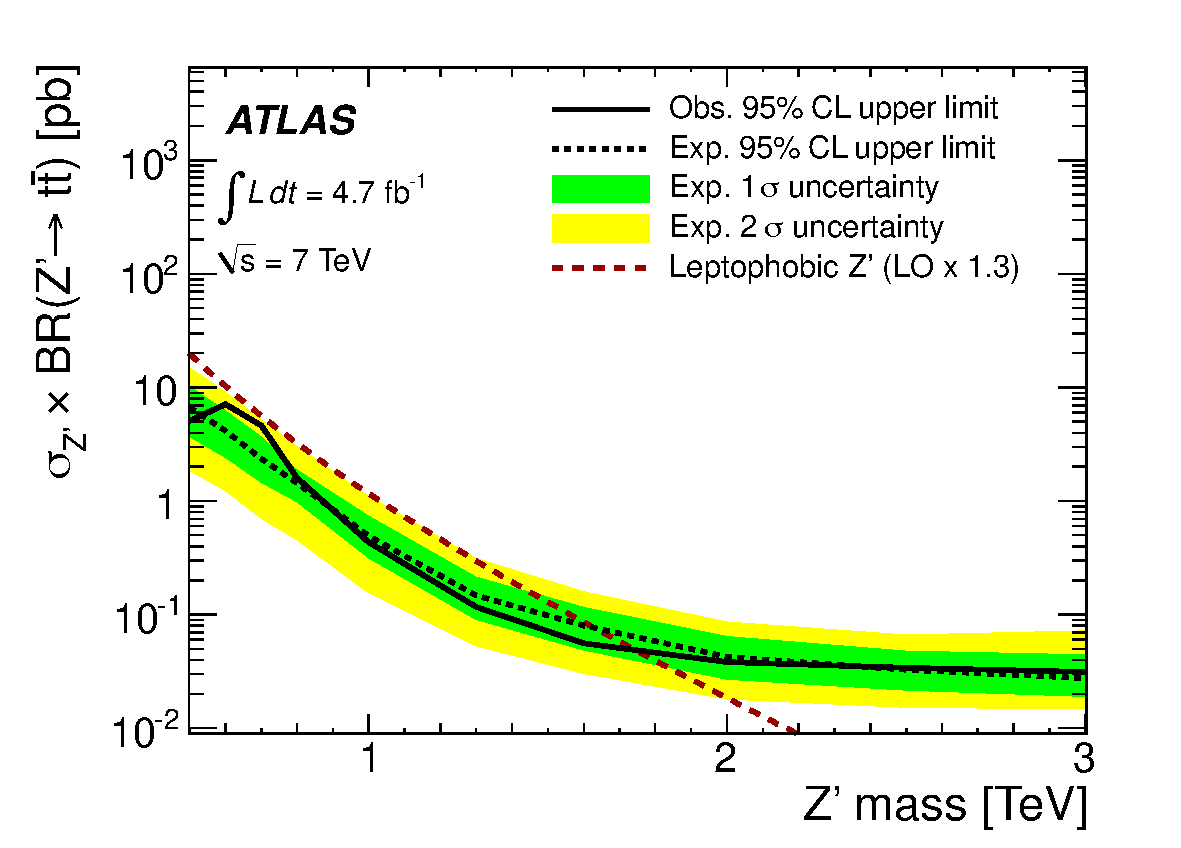
\includegraphics[width=0.75\textwidth]{PartTopQuark/Plots/fig_11a.pdf}

  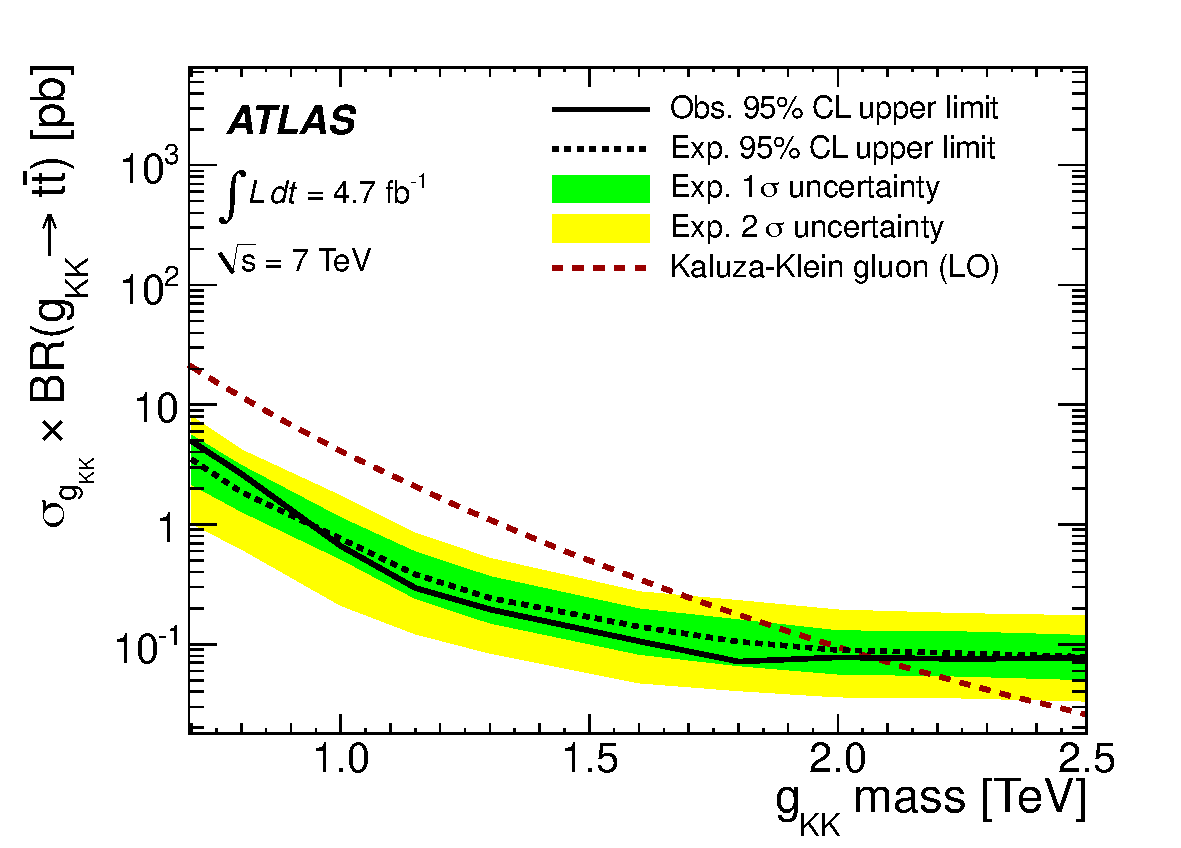
\includegraphics[width=0.75\textwidth]{PartTopQuark/Plots/fig_11b.pdf}
  \caption[Expected (dashed line) and observed (solid line) upper limits on the cross section times the \ttbar\ branching ratio of \Zprime\ (left) and Kaluza-Klein gluons (right) using the combined resolved and boosted selections.]{Expected (dashed line) and observed (solid line) upper limits on the cross section times the \ttbar\ branching ratio of \Zprime\ (left) and Kaluza-Klein gluons (right) using the combined resolved and boosted selections. The dark (green) and light (yellow) bands show the range in which the limit is expected to lie in \SI{68}{\percent} and \SI{95}{\percent} of pseudo-experiments, respectively, and the smooth solid (red) lines correspond to the predicted cross section times branching fraction. Both statistic and systematic uncertainties have been included~\cite{Boosted:ATLASExclusion7TeV}.}\label{fig:BoostedLimits}
\end{figure}


% !TEX root = ../Thesis.tex
\newcommand{\rphi}{\ensuremath{R\textrm{-}\phi}}
\newcommand{\T}{\ensuremath{\mathbf{T}}}
\newcommand{\Tms}{\ensuremath{\T_{\textrm{MS}}}}
\newcommand{\Tid}{\ensuremath{\T_{\textrm{ID}}}}
\newcommand{\C}{\ensuremath{\mathbf{C}}}
\newcommand{\Cms}{\ensuremath{\C_{\textrm{MS}}}}
\newcommand{\Cid}{\ensuremath{\C_{\textrm{ID}}}}
\newcommand{\kt}{\ensuremath{k_{\textrm{T}}}}
\newcommand{\kti}{\ensuremath{k_{\textrm{T},i}}}
\newcommand{\ktj}{\ensuremath{k_{\textrm{T},j}}}
\newcommand{\dij}{\ensuremath{\Delta_{ij}}}

\chapter{The LHC and the ATLAS Detector} \label{ch:Detector}

The Large Hadron Collider (LHC)~\cite{LHC} is a proton-proton ring collider located at the European Centre for Nuclear Research (CERN). The main LHC ring is housed in the tunnel which previously contained the Large Electron-Positron (LEP) collider. The LHC ring is \SI{27}{\kilo\meter} in circumference and located as deep as \SI{175}{\meter} underground. The LHC services seven different experiments located around the beam-pipe as shown in Figure~\ref{fig:DetectorLHCLayout}. There are four main experiments: A toroidal LHC apparatus (ATLAS, the experiment used for this thesis), the compact muon solenoid (CMS), a large ion collider (ALICE) experiment, and the LHC beauty (LHCb) experiment. 

ATLAS and CMS are general purpose detectors designed to support a varied physics programme, from SM physics like top quark measurements to BSM searches such as supersymmetry. ALICE and LHCb are more specialized experiments which focus on heavy ions and $B$-physics, respectively.

\begin{figure}[htbp]
  \centering
    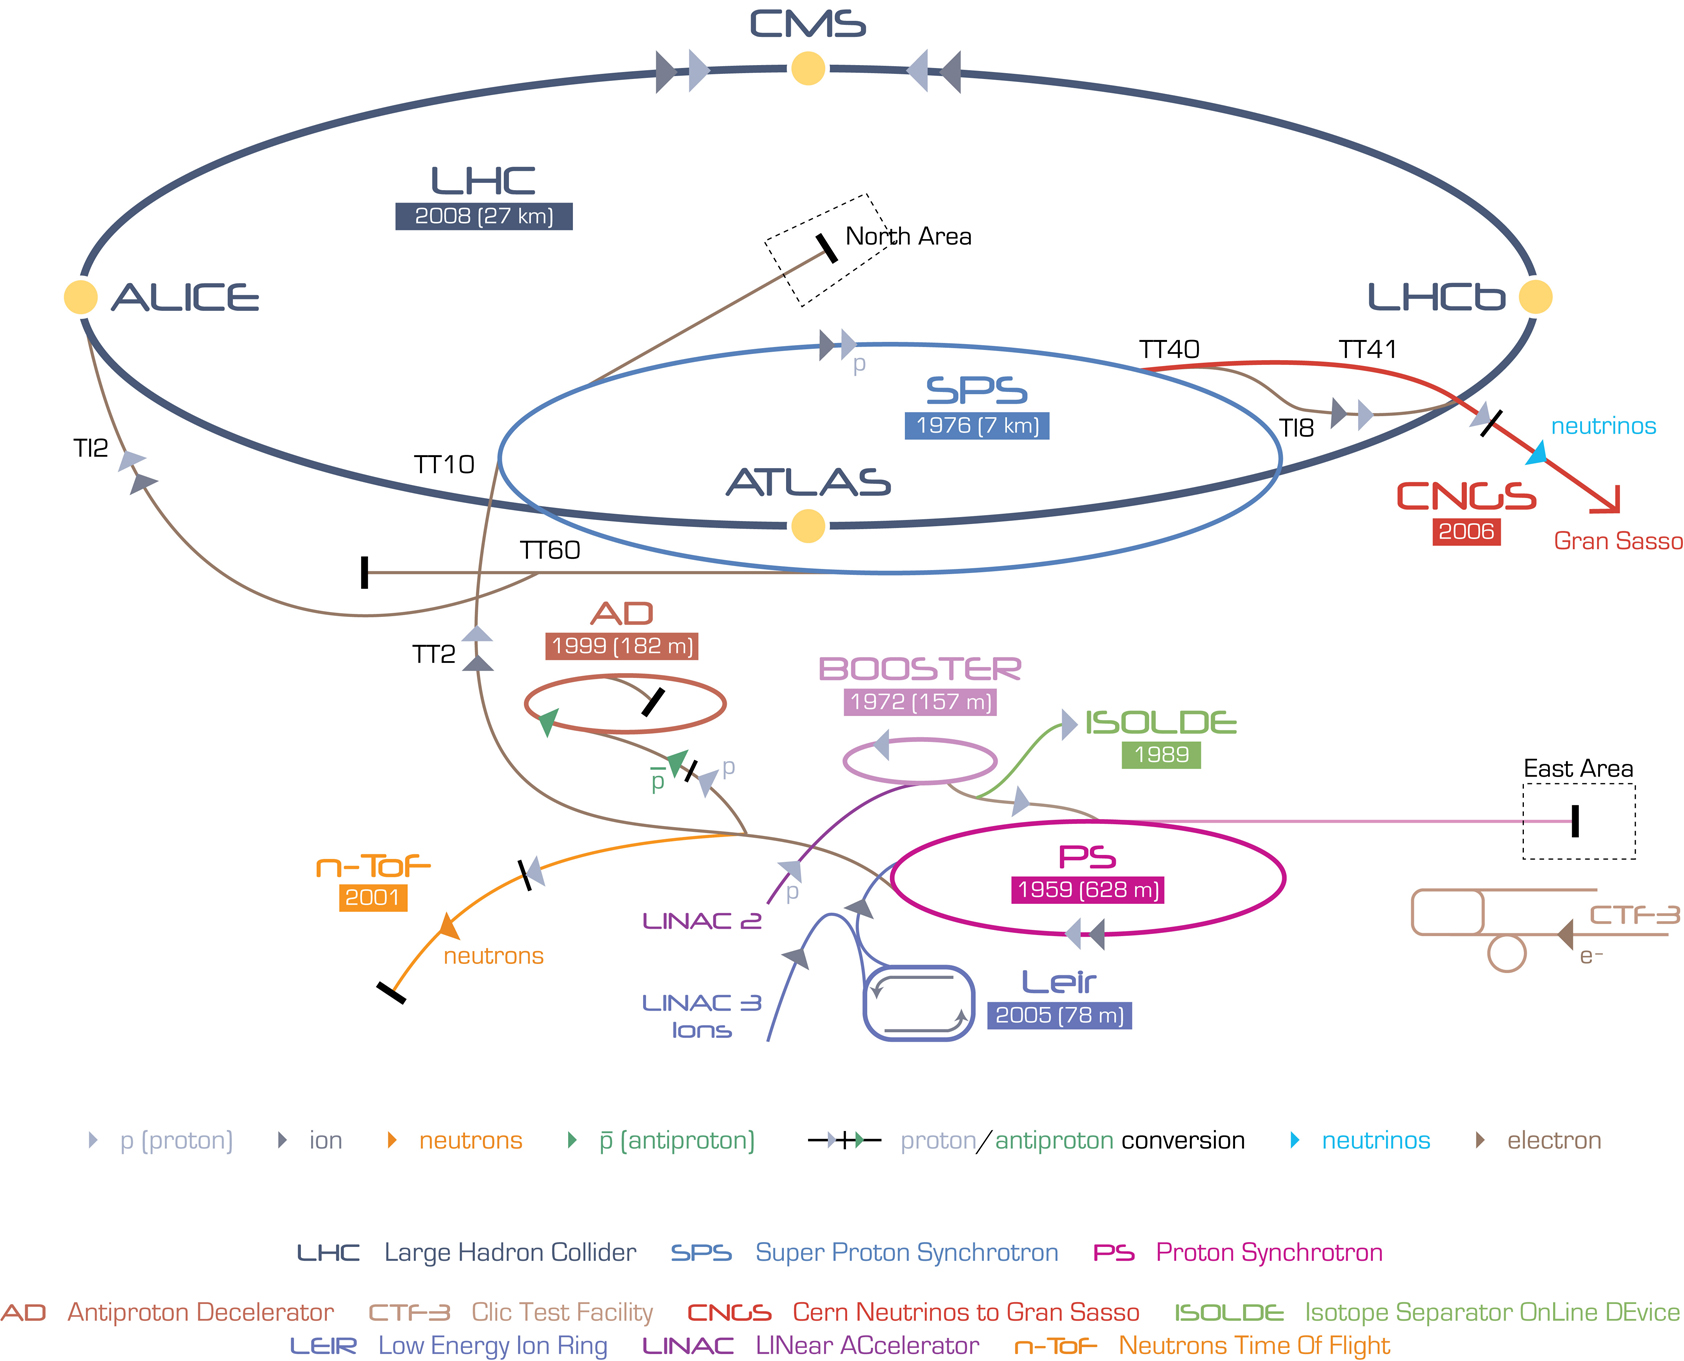
\includegraphics[width=0.95\textwidth]{PartDetector/Diagrams/Cern-Accelerator-Complex.jpg}
    \caption{The layout of CERN complex of experiments, note the main four LHC experiments located at different points around the ring.}
  \label{fig:DetectorLHCLayout}
\end{figure}

\section{The large hadron collider} \label{sec:the_large_hadron_collider}

The LHC accelerates two beams of protons in opposite directions and then collides them at the four interaction points where the experiments are located. The protons come from hydrogen gas where the orbiting electron is removed by an electric field, leaving behind a bare proton. The beam acceleration occurs in several stages exploiting smaller experiments present at CERN. During 2010 and 2011 protons were accelerated to a beam energy of \SI{3.5}{\TeV}, creating a centre of mass energy of \SI{7}{\TeV} and then \SI{4}{\TeV} per beam in 2012 for a centre of mass energy of \SI{8}{\TeV}. Each beam is made of multiple bunches of protons, with as many as hundreds of billions of protons in each bunch. Bunches are grouped into \textit{bunch trains} with a designed \textit{bunch spacing} of \SI{25}{\ns} between each of the bunches that compose a single train. The bunch spacing and size of the bunch can be altered to adjust the amount of collisions and time between collisions. During 2011 a \SI{50}{\ns} bunch spacing was used to allow for early low luminosity analyses to be performed. The variation in the number of colliding bunches is shown in Figure~\ref{fig:DetectorBunchesColliding}.

\begin{figure}[htbp]
  \centering
    \begin{subfigure}[b]{0.95\textwidth}
      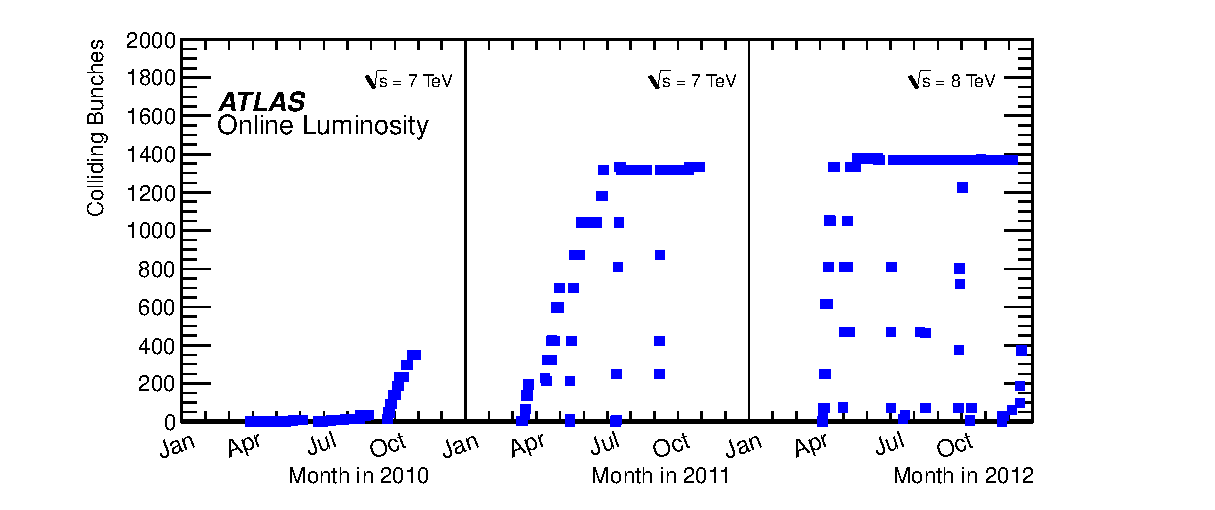
\includegraphics[width=\textwidth]{PartDetector/Plots/BunchesCollidingPerTime.eps}
      \caption{The number of bunches colliding per unit time at the LHC for the 2010, 2011 and 2012 $pp$ collision periods.}
      \label{fig:DetectorBunchesColliding}
    \end{subfigure}
  
    \begin{subfigure}[b]{0.95\textwidth}
      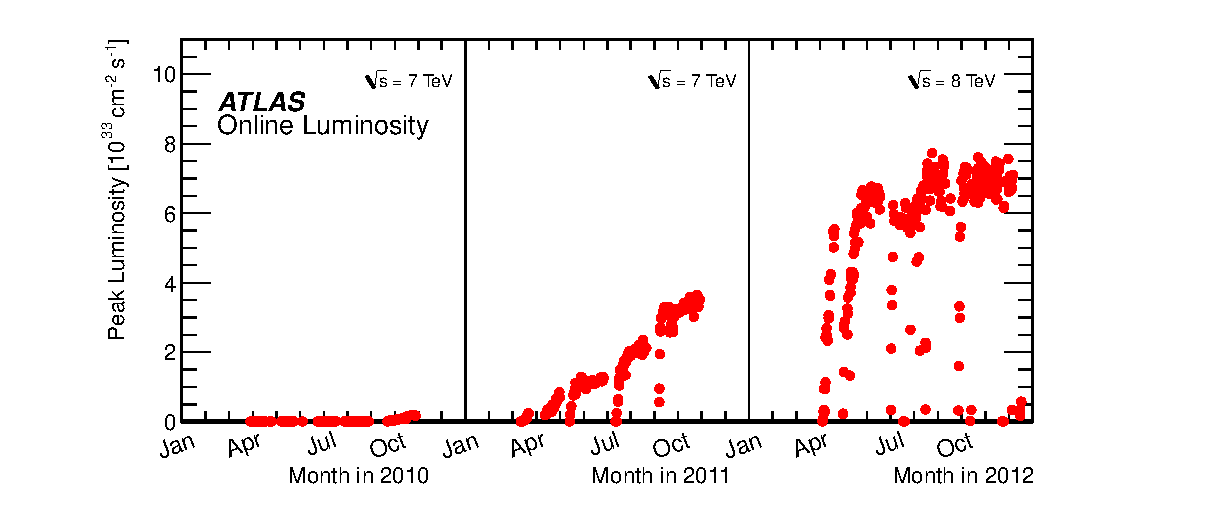
\includegraphics[width=\textwidth]{PartDetector/Plots/PeakLuminosityVsTime.eps}
      \caption{The peak luminosity per unit time at the LHC for the 2010, 2011 and 2012 $pp$ collision periods.}
      \label{fig:DetectorPeakLumi}
    \end{subfigure}
    \caption{Shown in~\subref{fig:DetectorBunchesColliding} is the number of bunches colliding at the LHC and \subref{fig:DetectorPeakLumi} the peak luminosity per unit time~\cite{Detector:LuminosityResults}.}
  \label{fig:DetectorPerformance}
\end{figure}

The acceleration of the proton beams occurs in several stages in different accelerators. The beams are first accelerated in a linear collider (LINAC 2) to an energy of \SI{50}{\MeV} before being injected into the proton synchrotron booster (PSB). The beams are then boosted to \SI{1.4}{\GeV} by a varying magnetic field in the circular PSB. Beams are then passed into the proton synchrotron (PS) and then the super proton synchrotron (SPS) where the beam energy increases to \SI{26}{\GeV} and then \SI{450}{\GeV}. At this stage the beam is injected into the LHC and then accelerated to the final desired energy. The design energy is \SI{7}{\TeV} per beam for a total of \SI{14}{\GeV} centre of mass energy. The whole process can take a couple of hours, from the initial injection of the protons to stable beam conditions in the LHC.

As bunches overlap, the protons that make up the bunches interact, each interaction is known as an event. The number of events is proportional to the instantaneous luminosity $\Lagr$ of the collider. $\Lagr$ is a measure of the flux of particles per unit area per unit time can be defined as:

\begin{equation}
  \Lagr=fn_{b}\frac{N_1 N_2}{A}
\end{equation}
%
where $f$ is the frequency of revolution of the beam, $n_b$ the number of colliding pairs of bunches in the beam, $N_1$ and $N_2$ are the number of particles in each colliding bunch and $A$ is the cross section of the beam~\cite{Luminosity}. The peak luminosity evolution at the LHC is shown in Figure~\ref{fig:DetectorPeakLumi}.

The total amount of data collected is measured by the integrated luminosity $\Lagr_{\textrm{int}}$ defined as the time integral of $\Lagr$. Integrated luminosity has units of inverse area, usually expressed in terms of barns (\si{\barn})\footnote{\SI{1}{\per\barn}=\SI{e-28}{\per\square\meter}}. The probability for a given process to occur is expressed as the cross section $\sigma$ and the total number of events which proceed via said process is defined as:
%
\begin{equation}
  \sigma\int\Lagr \dd t
\end{equation}

The integrated luminosity delivered by the LHC and collected by the ATLAS detector in 2011 and 2012 is shown in Figure~\ref{fig:DetectorIntLumi}. The ATLAS detector does not record all data delivered by the LHC; approximately $6.5\%$ was not recorded.

\begin{figure}[htbp]
  \centering
    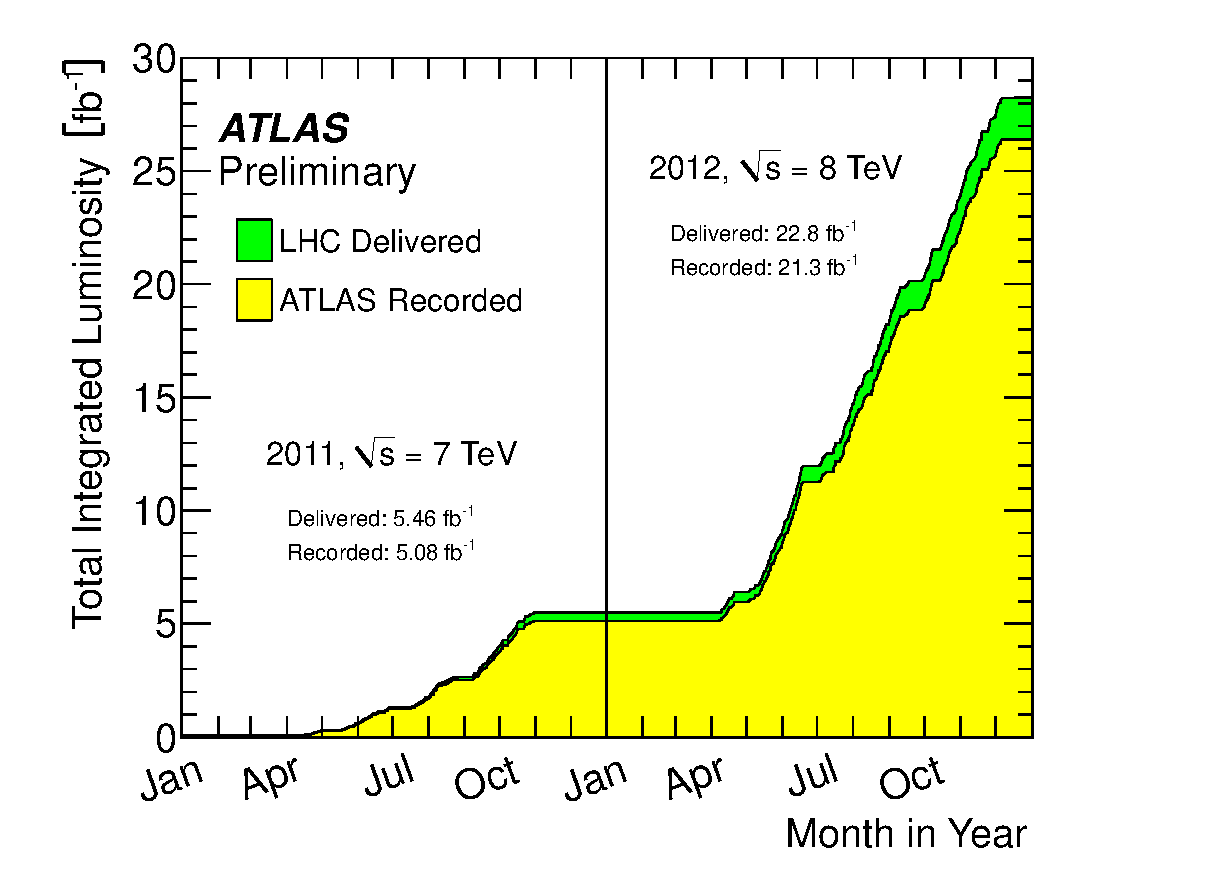
\includegraphics[width=0.70\textwidth]{PartDetector/Plots/IntegratedLuminosity20112012.eps}
    \caption{Distribution of the total integrated luminosity delivered by the LHC and the recorded by ATLAS for the 2011 and 2012 $pp$ collision period~\cite{Detector:LuminosityResults,Luminosity}.} \label{fig:DetectorIntLumi}
\end{figure}

\subsection{Pile-up}

Due to the large number of interactions and the short time between collisions, multiple events can overlap into a single event. This has detrimental effects on physics analyses and is a determining factor in setting the instantaneous luminosity with which to perform data collection. This overlapping effect is collectively known as pile-up and is categorized into two types: in-time pile-up, where multiple $pp$ collisions occur during the same bunch crossing; and out-of-time pile-up, where the electric signals produced by previous collisions still remain to be read-out. This occurs when the time spacing between interactions is smaller than the read-out speed of the electronics. The number of interactions per crossing $\mu$ is shown in Figure~\ref{fig:DetectorBunchCrossingInteractions}, note that on average approximately thirty interactions occurred per bunch crossing in 2012. In comparison, in 2011 the average interactions per bunch crossing $\langle\mu\rangle$ varied from 5 in early 2011 to 15 at the end of the year.

\begin{figure}[htbp]
  \centering
    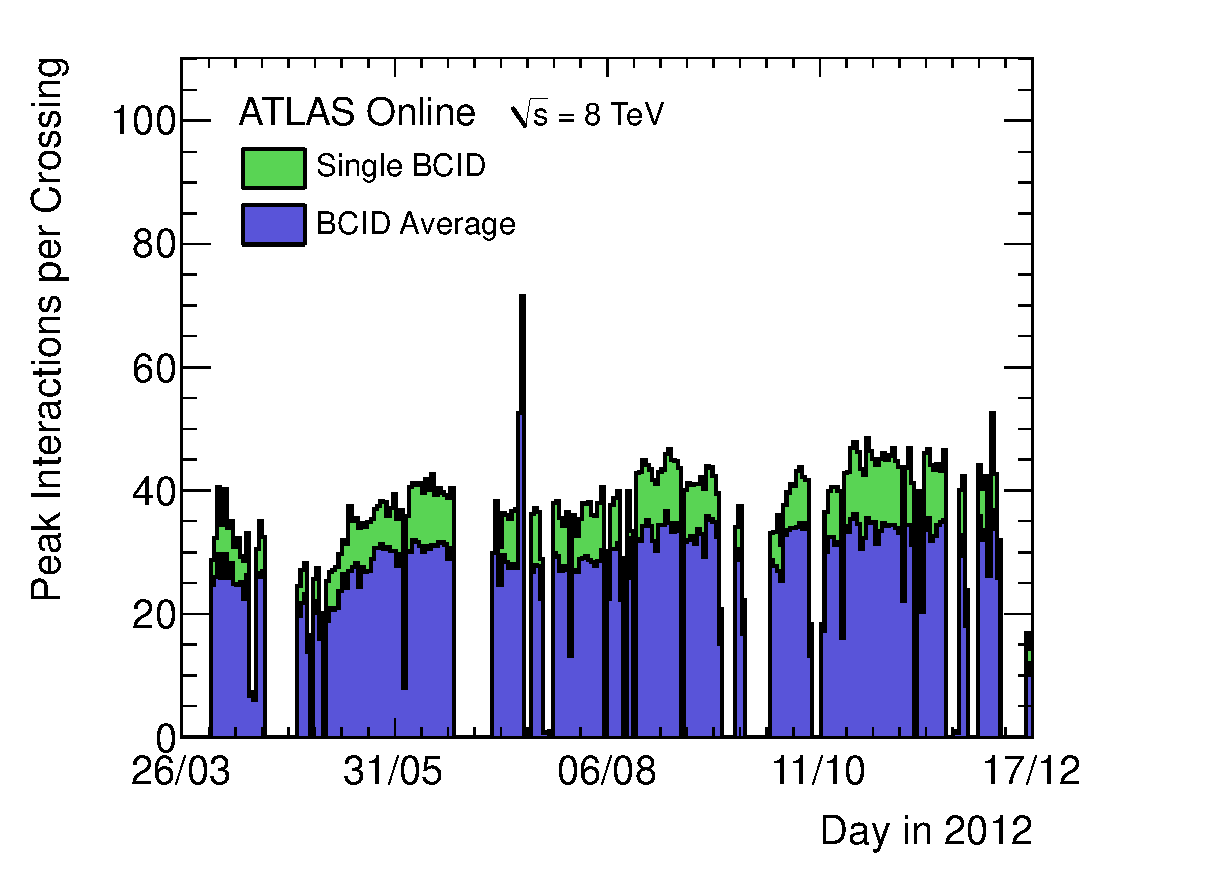
\includegraphics[width=0.70\textwidth]{PartDetector/Plots/peakBothMuByDay.eps}
    \caption[Number of interactions per bunch for the 2012 $pp$ data-taking period at ATLAS per day.]{Number of interactions per bunch for the 2012 $pp$ data-taking period at ATLAS per day. Both the average number of interactions for all bunches and the maximum number of interactions are shown~\cite{Detector:LuminosityResults}.}
  \label{fig:DetectorBunchCrossingInteractions}
\end{figure}

\section{The ATLAS detector} \label{sec:the_atlas_detector}

The ATLAS~\cite{Detector:ATLASExperimentGeneral} experiment is a general-purpose detector which wraps around the IP providing large angular coverage. ATLAS is approximately cylindrical with a diameter of \SI{25}{\meter}, a total length of \SI{44}{\meter} and weighs \SI{7000}{\tonne}. The detector is made of several layers of instrumentation located at successively increasing radii as shown in Figure~\ref{fig:ATLASOverviewFigure}:

\begin{enumerate}
  \item \textbf{Inner Detector}: Located nearest to the beam-pipe and designed to measure the track of charged-particles.
  \item \textbf{EM Calorimeter}: Used for identification and measurement of electrons and photons.
  \item \textbf{Hadronic Calorimeter}: Used for the measurement of hadronic activity from hadronizing partons and missing transverse energy.
  \item \textbf{Muon Spectrometer}: The outermost detection layer, used for muon identification and measurement.
\end{enumerate}

Between these detection layers are magnets responsible for bending the path of the charged particles for the purpose of momentum measurement and particle identification. Triggering and data acquisition (TDAQ) systems also form part of the detector for the purposes of recording the data signals coming from the tracking and measurement systems. A brief description of these is provided in the coming sections. For a more detailed technical description of the detector and all subsystems see~\cite{Detector:ATLASExperimentGeneral}.

Lepton plus jets \ttbar\ events produce a final state that includes hadronic activity, electrons, muons and missing energy, so all elements of the detector are used in the reconstruction of such events. Additionally, the match \xsm\ tagger which is central to this thesis, relies on the reconstruction and fitting of ID tracks and MS tracks. A detailed description of this algorithm is provided in Section~\ref{sec:DetectorSTACO}.

\begin{figure}[htbp]
  \centering
    \includegraphics[width=0.90\textwidth]{PartDetector/Diagrams/ATLAS_Overall.eps}
    \caption{An overview diagram of the ATLAS experiment. Shown are all detection and tracking systems and the toroid magnet which encompasses them. Note also the muon system on the outside of the detector~\cite{Detector:ATLASExperimentGeneral}.}
  \label{fig:ATLASOverviewFigure}
\end{figure}

A cylindrical coordinate system as used by all ATLAS publications has been adopted here. The coordinate system is constructed so that the $z$-axis is parallel to the beam axis. The $x$-axis is positive in the direction going from the IP to the centre of the LHC ring, and the positive $y$-axis points upwards. Thus the $x$-$y$ plane is transverse to the beam direction. All transverse variables such as the transverse momentum \pt, transverse energy \Et\ and missing transverse energy \met\ are measured along this plane. The distance perpendicular to the beam-pipe is denoted by $R$, the azimuthal angle $\phi$ is measured around the beam axis, and the polar angle $\theta$ is the angle from the beam axis. The pseudorapidity is defined as $\eta=-\ln\tan(\theta/2)$. The distance in the $\eta$-$\phi$ plane between two objects is denoted by $\Delta R$ and defined as $\Delta R = \sqrt{\Delta\eta^{2}+\Delta\phi^{2}}$. Finally side A of the detector is defined as the positive $z$ side and side C is the negative $z$.  The transverse impact parameter $d_{0}$ is defined as the distance of closest approach (perigee) of a track to the primary vertex, and the longitudinal impact parameter $z_{0}$ is the distance in $z$ between the perigee and the primary vertex.

\subsection{Inner detector} \label{subsec:DetectorID}
The inner detector (ID), shown in Figure~\ref{fig:DetectorIDOverview}, is a tracking detector located closest to the beam-pipe and used for momentum and impact parameter measurement, vertex and track reconstruction, and particle identification. The ID is designed to provide hermetic high-resolution tracking in the range $\aeta<2.5$.

\begin{figure}[htbp]
  \centering
    \includegraphics[width=0.85\textwidth]{PartDetector/Diagrams/ATLAS_ID.eps}
    \caption{Drawing of the ATLAS inner detector~\cite{Detector:ATLASExperimentGeneral}.}
  \label{fig:DetectorIDOverview}
\end{figure}

The entire ID is contained within the central solenoid (CS) that generates a \SI{2}{\tesla} magnetic field for the purpose of momentum measurement. The trajectory of a charged particle is bent in the presence of a magnetic field by an amount proportional to the momentum of the particle
%
\begin{equation}
  r=\frac{\pt}{qB}
\end{equation}
%
where $r$ is the bending radius, \pt\ is the transverse momentum of the particle, $q$ is the charge of the particle, and $B$ is the magnetic field strength. Thus the momentum of the particle can be measured by reconstructing its trajectory through the detector. A particle with larger \pt\ would have a more straight trajectory than a particle with low \pt\ in the same magnetic field. For a central track with $\pt=\SI{5}{\GeV}$ the relative resolution on the measured transverse momentum is $\sim\SI{1.5}{\percent}$~\cite{Detector:ATLASExperimentGeneral}.

The reconstruction of interaction vertices is paramount, particularly when considering the large amount of pile-up observed at ATLAS. Interaction vertices are reconstructed by fitting all reconstructed tracks to a point. The primary vertex (PV) is then defined as the vertex with the largest amount of momentum associated with it. The reconstruction of secondary interaction vertices is used for the identification of short-lived particles such as $b$-hadrons and $\tau$.

\begin{figure}[htbp]
  \centering
  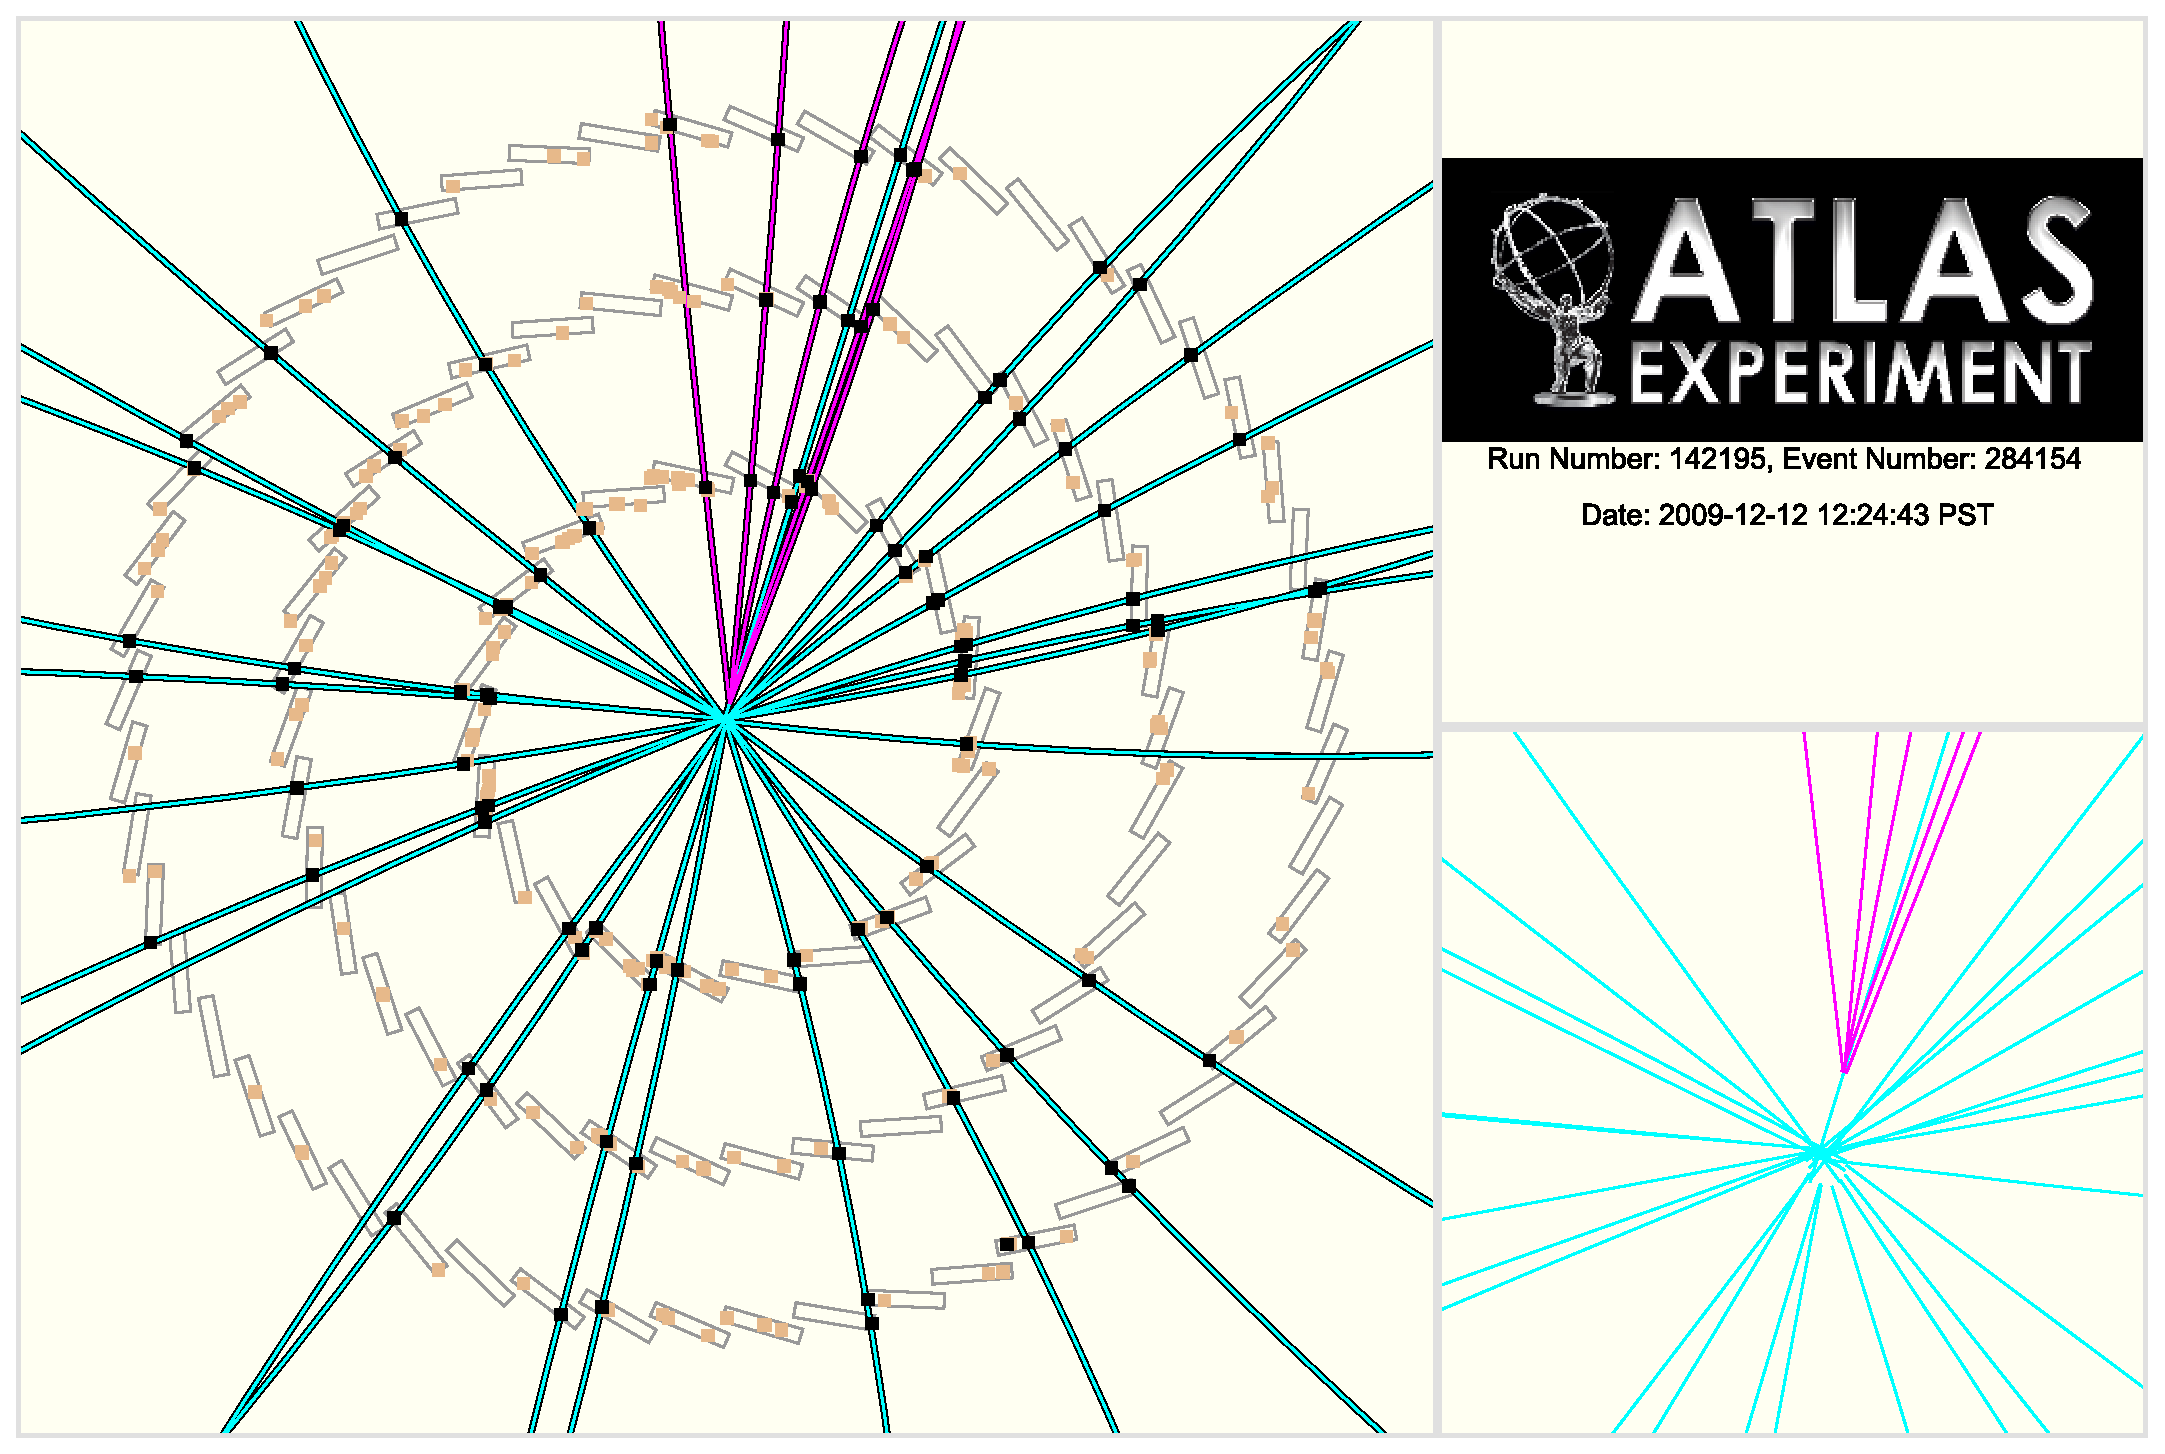
\includegraphics[width=0.75\textwidth]{PartDetector/Diagrams/fig_14.eps}
  \caption[An event display of an event as reconstructed by the ATLAS inner detector.]{An event display of an event as reconstructed by the ATLAS inner detector~\cite{Detector:ATLASExperimentGeneral}. Shown are the results of the vertexing algorithm where each line represents a track. the purple tracks have been fitted to a secondary vertex.}
  \label{fig:DetectorEventDisplayID}
\end{figure}

The ID is made of three separate tracking and detection systems located at increasing radii away from the beam-pipe, the full arrangement can be seen in Figure~\ref{fig:DetectorIDQuarter}, and a plane-view is shown in Figure~\ref{fig:DetectorIDTransverse}.

\begin{figure}
  \centering
    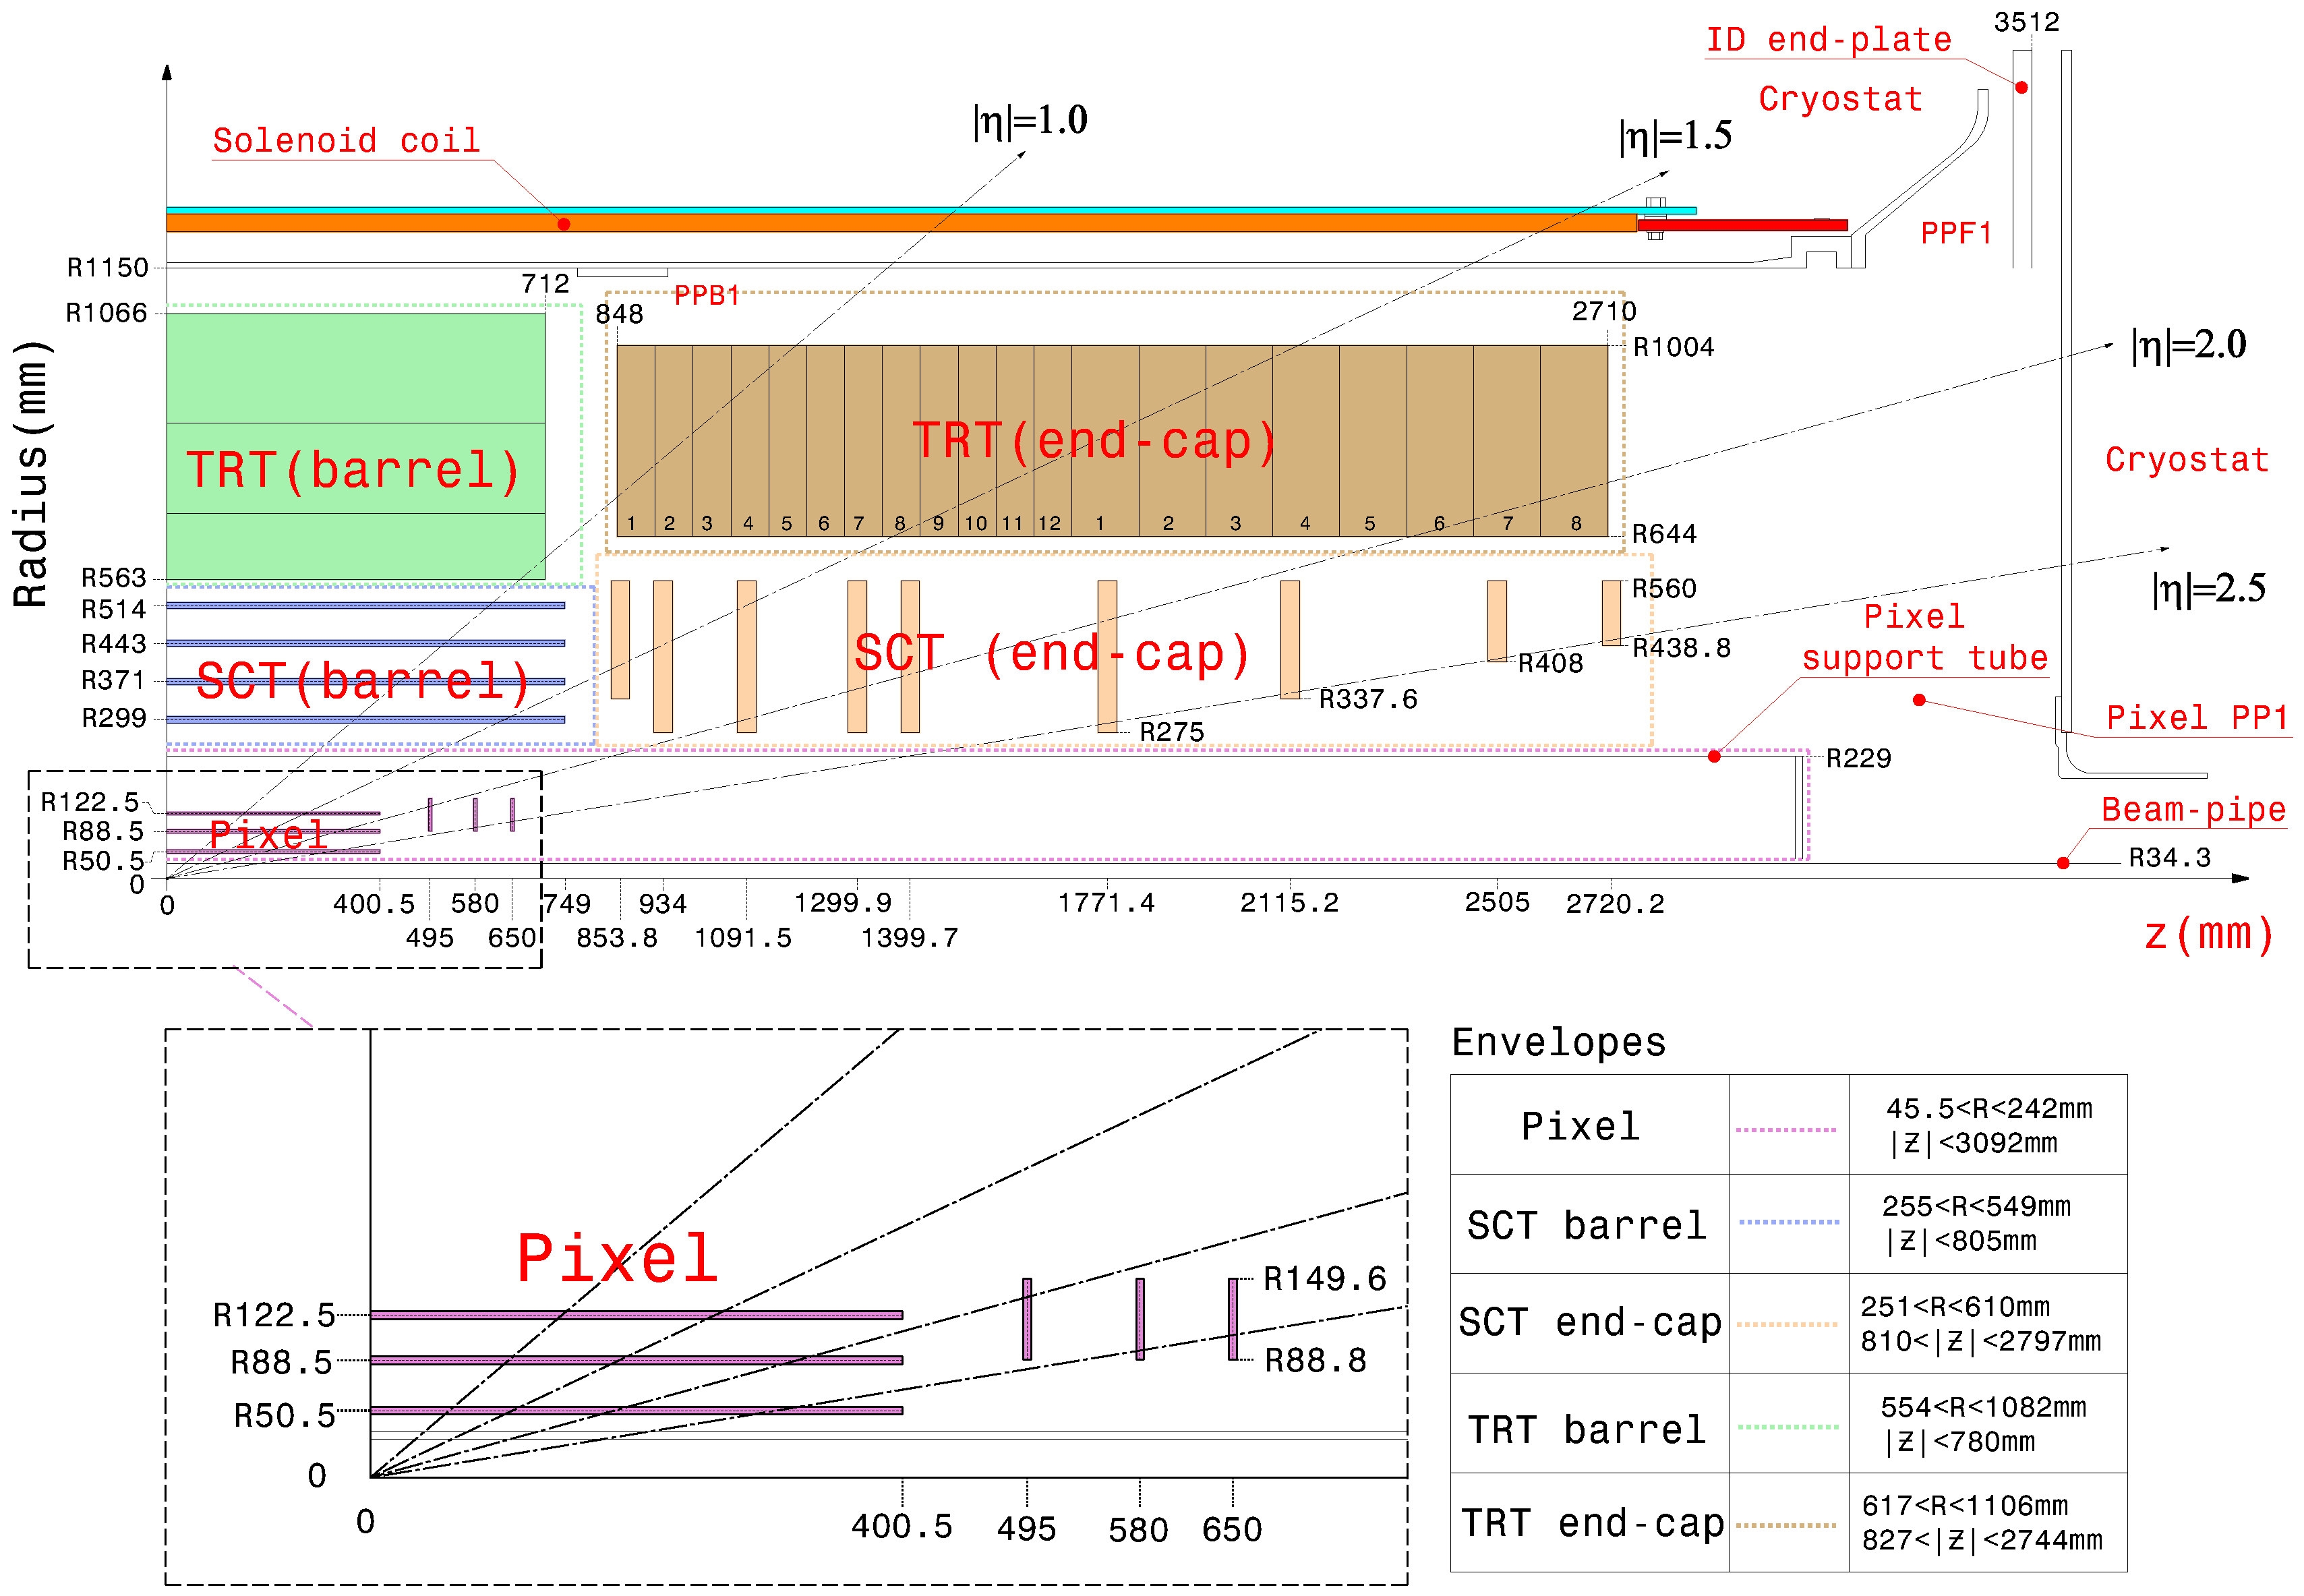
\includegraphics[width=0.75\textwidth]{PartDetector/Diagrams/Detector_ID_QuarterView.eps}
    \caption[Plan-view of a quarter-section of the ATLAS ID showing the major detector elements with its active dimensions and envelopes.]{Plan-view of a quarter-section of the ATLAS ID showing the major detector elements with its active dimensions and envelopes~\cite{Detector:ATLASExperimentGeneral}. Note also the $\eta$ markers showing the maximum coverage up to $\eta=2.5$.}
  \label{fig:DetectorIDQuarter}
\end{figure}
  
\begin{figure}
  \centering
    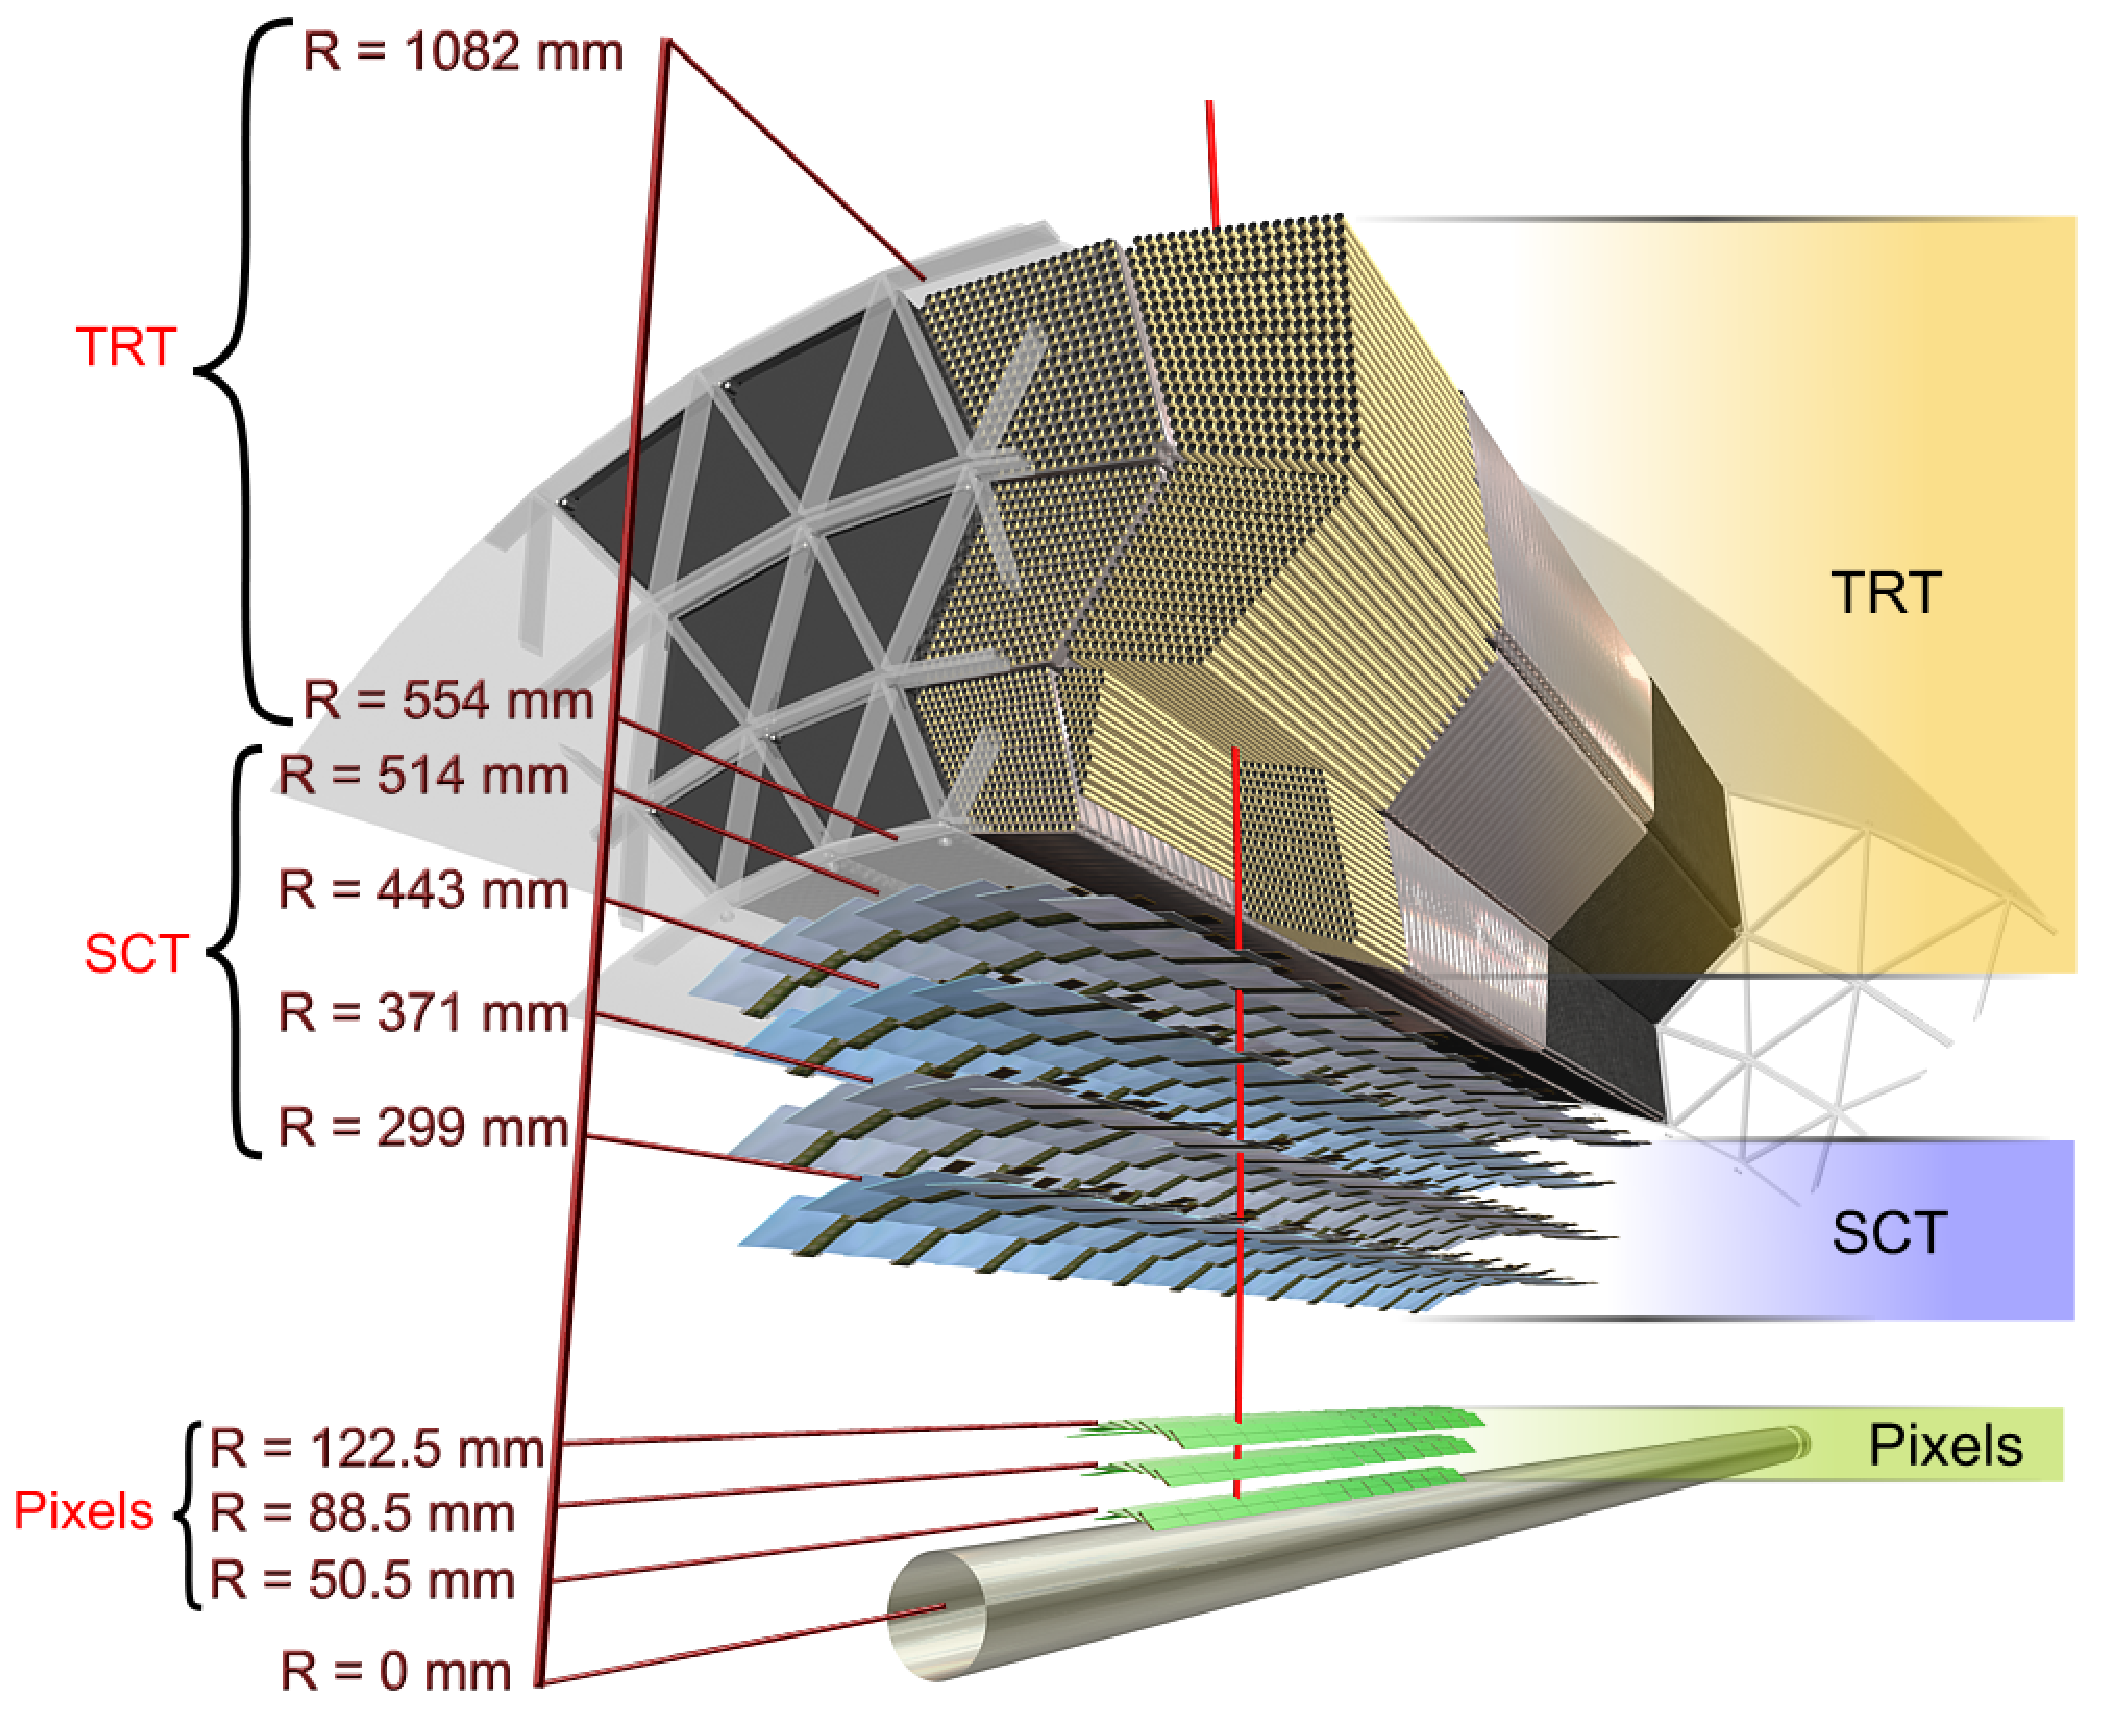
\includegraphics[width=0.75\textwidth]{PartDetector/Diagrams/ID_3D_Overview.eps}
    \caption[A drawing in the transverse plane of the ATLAS ID showing all major detection elements in the barrel regions.]{A drawing in the transverse plane of the ATLAS ID showing all major detection elements in the barrel regions~\cite{Detector:ATLASExperimentGeneral}. A charged particle track is shown traversing all the detector elements as a solid line.}
  \label{fig:DetectorIDTransverse}
\end{figure}

\subsubsection{Pixel detector}

The pixel detector is located nearest to the beam-pipe and provides high-granularity and precision for secondary vertex reconstruction. As a charged particle passes through a silicon pixel, an electron-hole pair is created. The electron and hole begin drifting in opposite directions under the influence of a voltage, and the charge is then read out as a \emph{hit} through an electrode. The pixel detector consists of three silicon pixel sensor layers in the barrel region located at approximately \SIlist{5;9;12}{\cm} from the IP, and three disks at each side located at constant $R$ providing coverage up to $\aeta<2.5$. The barrel modules are overlapped in a turbine pattern to provide hermetic coverage. In the barrel region the modules provide an intrinsic resolution of \SI{10}{\um} in \rphi\ and \SI{115}{\um} in $z$~\cite{Detector:ATLASExperimentGeneral}. The disk sections have an intrinsic resolution of \SI{10}{\um} (\rphi) and \SI{115}{\um} ($R$).

\subsubsection{Semiconductor tracker}
The semiconductor tracker (SCT) located in the intermediate radius range is designed to provide eight hits per track contributing to the measurement of momentum, impact parameter, and vertex position. The SCT is made of four layers of stereo-pair silicon micro-strip sensors in the barrel region at increasing radii. The intrinsic resolutions are \SI{17}{\um} (\rphi) and \SI{580}{\um} ($z$). At the end-caps nine disks of silicon micro-strip modules provide large pseudorapidity coverage with a resolution of \SI{17}{\um} (\rphi) and \SI{580}{\um} ($R$)~\cite{Detector:ATLASExperimentGeneral}.

\subsubsection{Transition radiation tracker}
The transition radiation tracker (TRT) is the outermost tracking layer of the ID, and acts as both a tracker and transition radiation detector. Transition radiation (TR) is produced when a charged particle crosses the boundary between two materials with different dielectric constants. The probability of producing TR photons depends on the Lorentz factor of the particle $\gamma=E/m$. Thus for two particles of the same energy, a lighter particle will, on average, emit more ionization than a heavier particle.

The TRT is designed to provide up to \num{36} hits per track using straw-tube sensors. Each straw is \SI{4}{\mm} in diameter and is made of two \SI{35}{\micro\meter} thick Kapton multi-layer films bonded back-to-back. At the centre of each straw is a gold-plated tungsten wire with a diameter of \SI{31}{\micro\meter}. Each straw is filled with a mixture of gas (\SI{70}{\percent} xenon, \SI{27}{\percent} $\textrm{CO}_{2}$ and \SI{3}{\percent} $\textrm{O}_2$). The tubes are surrounded by polypropylene-polyethylene fibres that act as radiators and allow for the production of TR, which later ionizes the gas mixture and is read-out through the gold-plated wire.

In the barrel, the \SI{144}{\cm} long straw-tubes are arranged in modules which contain between \num{329} and \num{793} straws. The end-cap disks are made of radially distributed \SI{36}{\cm} long straw-tubes. Each tube provides an intrinsic resolution of \SI{130}{\um} along its length~\cite{Detector:ATLASExperimentGeneral}. The combination of a large number of hits over a large radius allows measurements in the TRT to be made with an accuracy that can complement those made by the pixel detector.

\subsection{Calorimetry}
The ATLAS calorimeter is responsible for the measurement of the energy of particles that emerge from the event. Sampling calorimeters are used for this purpose, layers of absorber material (passive) are placed in the path of the particles forcing them to interact and shower. The amount of energy lost by the incident particle depends on the type of material the particle traverses, the energy of the particle, and the type of particle. At high energy, electrons lose energy predominantly via Bremsstrahlung, while photons lose energy via pair production. The characteristic length associated with this energy loss is a material property known as the radiation length $X_0$.

For electrons, the energy as a function of material length traversed is
%
\begin{equation}
  E=E_0e^{-x/X_0}
\end{equation}
%
where $E_0$ is the initial energy, $x$ is the distance traversed, and $E$ is the energy of the particle at $x$. As an electron traverses one $X_0$ of material, its energy is reduced by a factor of $1/e$. For photons, the average number of photons traversing through a material length $x$ is reduced exponentially by a factor of $\frac{7}{9}X_0$. Thus the longitudinal length of the shower is proportional to the logarithm of the energy of the incoming particle.

The number of shower particles changes as a function of the interaction length $\lambda_{\textrm{int}}$ as
%
\begin{equation}
  N=N_{0}e^{-x/\lambda_{\textrm{int}}}
\end{equation}
%
where $N$ is the number of shower particles at length $x$ and $N_{0}$ is the initial number of incident particles. This is the characteristic length used when discussing the construction of the hadronic calorimeter. For a given material the $\lambda_{\textrm{int}}$ is much larger than $X_{0}$, therefore hadronic showers tend to be much broader and deeper than EM showers. Note that on average $1/3$ of the particle content of hadronic showers is electromagnetic, mostly due to pion decay into photons.

The energy of the resulting shower is measured by some sampling material (active) located behind the absorbers, this energy is proportional to the energy of the incident particle.

The type and thickness of material used is varied through the pseudorapidity range to improve energy measurement and reduce punch-through of particles into the muon system behind. Due to the intense radiation produced during collisions, radiation hardness is also an important factor in material choice.

The ATLAS calorimeter consists of the EM calorimeter, designed to measure photons and electrons covering $\aeta<3.2$; the hadronic calorimeter (HCal), which measures hadronic activity at $\aeta<3.2$; and the forward calorimeter (FCal) which provides energy measurement capability in at $3.1<\aeta<4.9$. As can be seen in Figure~\ref{fig:ATLASCalorimetryOverall}, the calorimetry envelopes the ID and CS providing hermetic coverage symmetric in $\phi$. This is particularly important for the measurement of \met\ resulting from weakly interacting particles escaping the detector.

\begin{figure}[htbp]
  \centering
  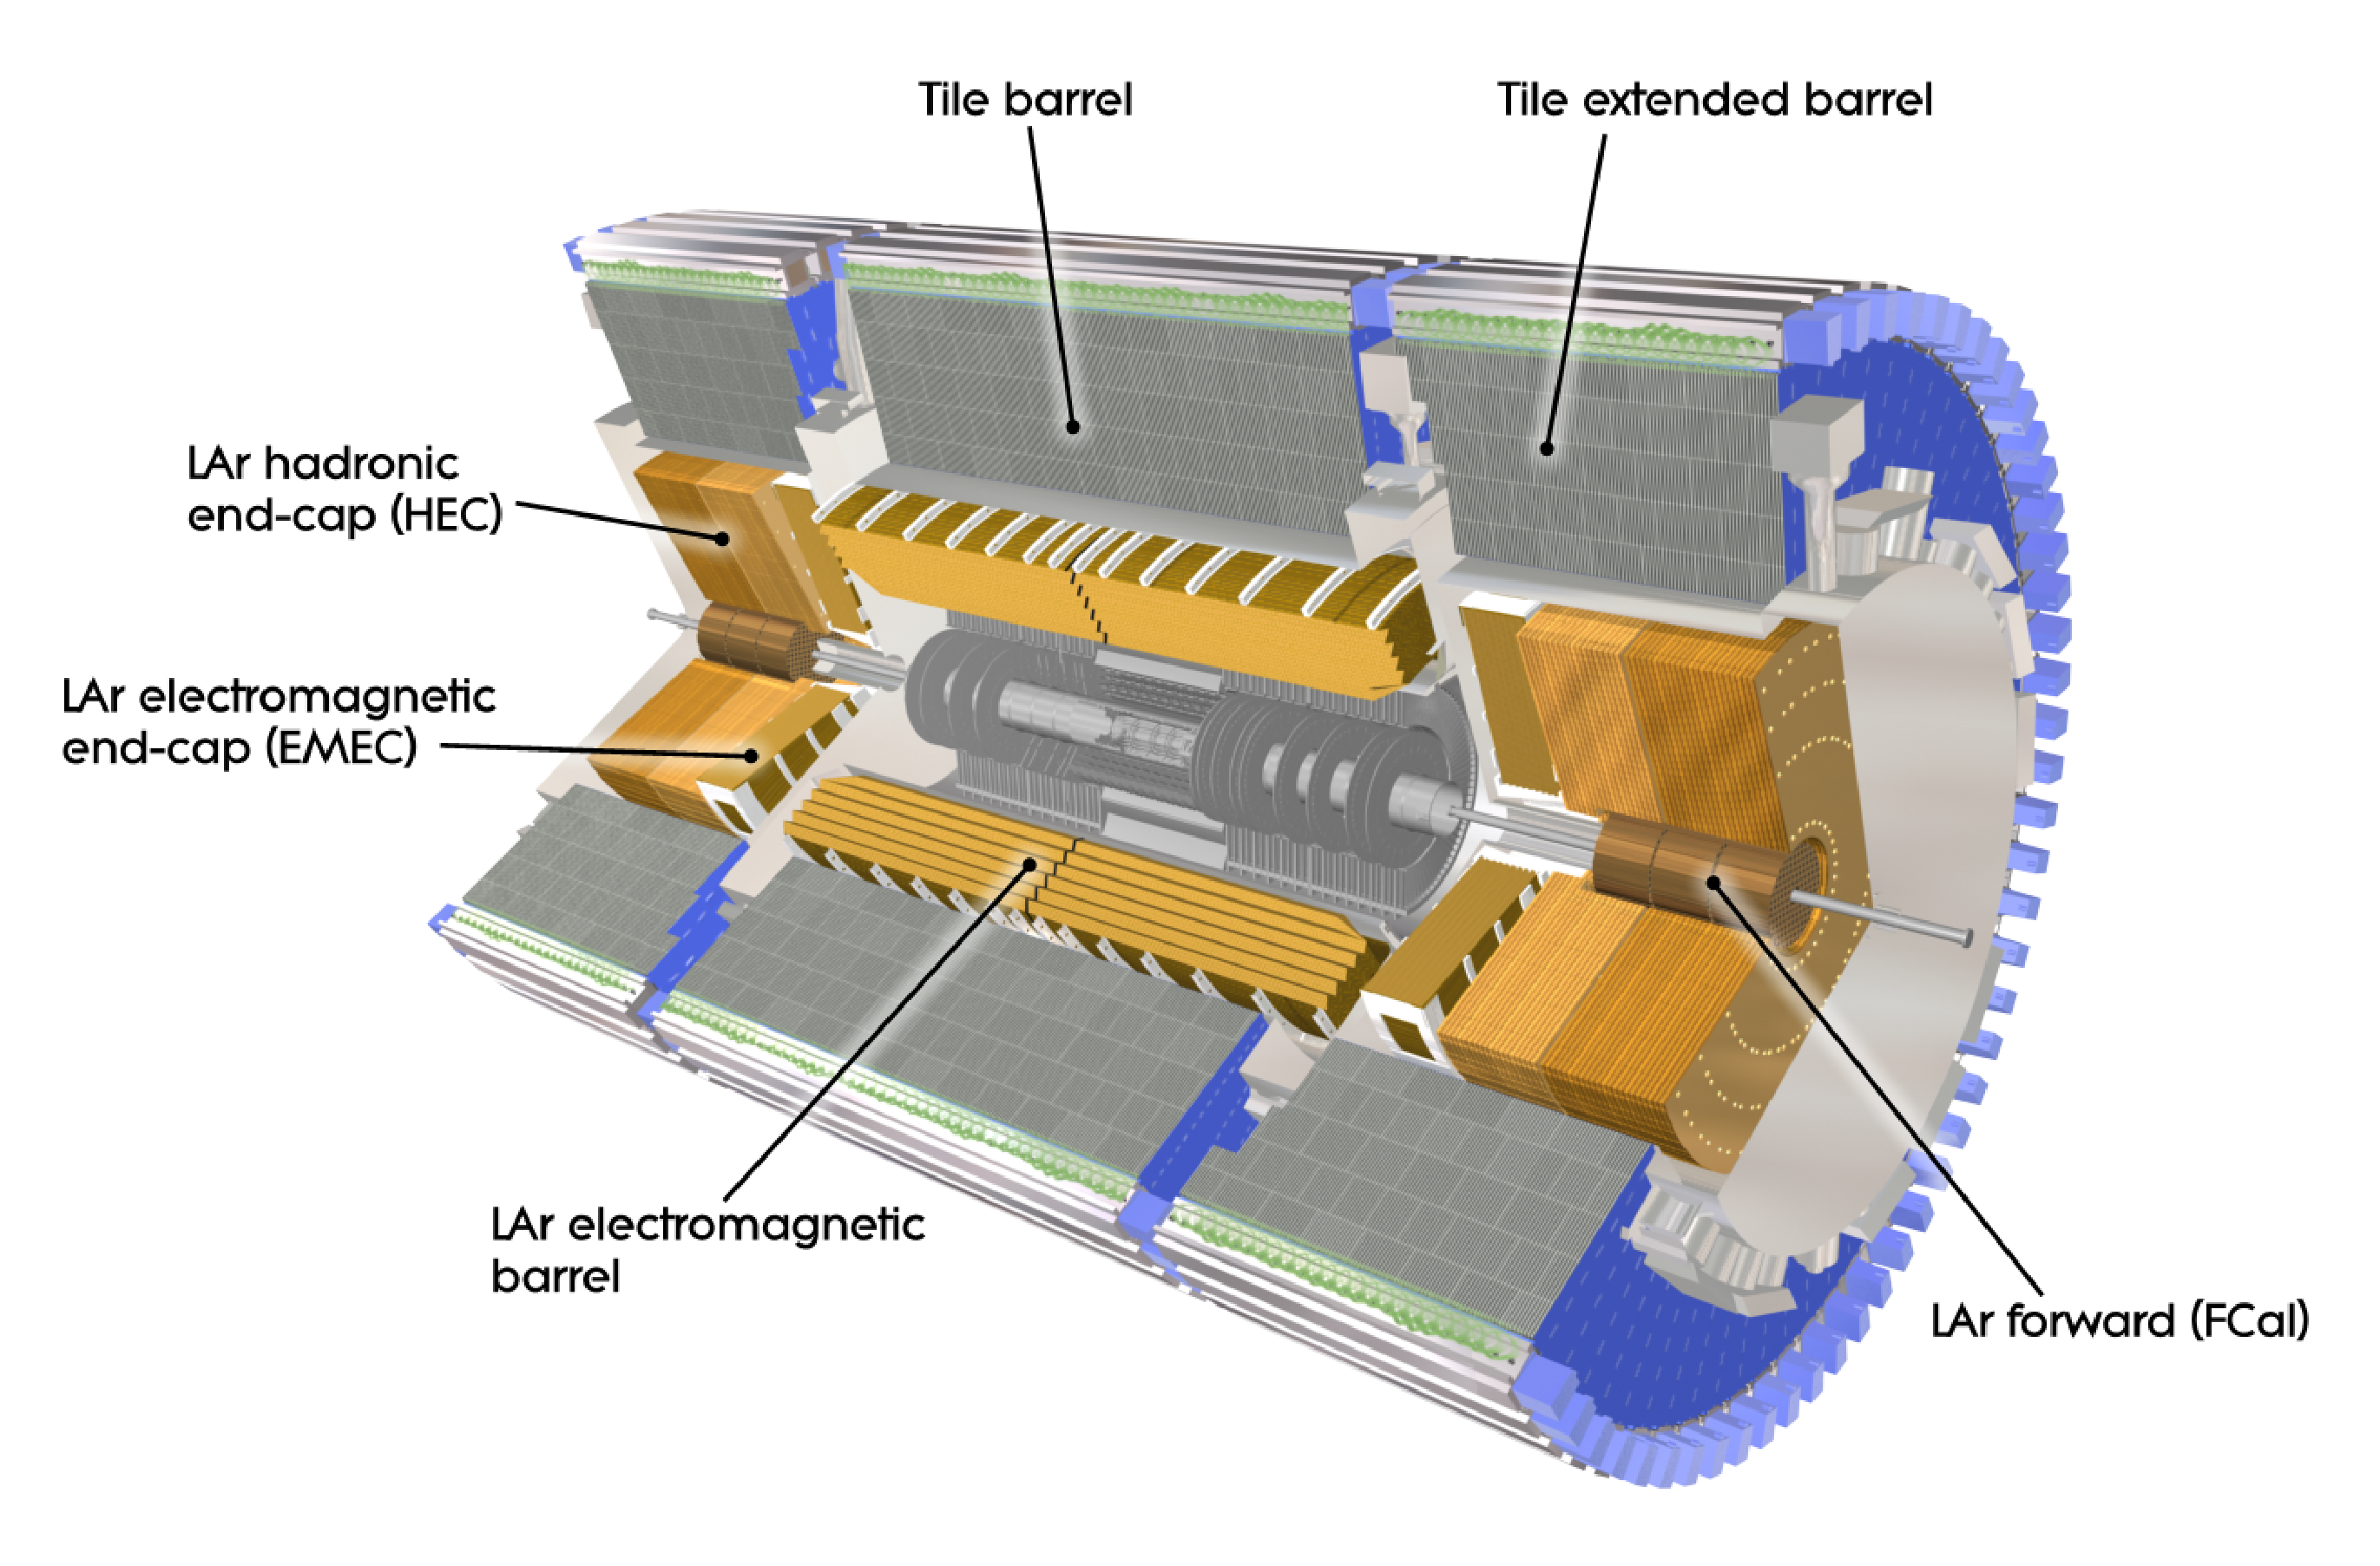
\includegraphics[width=0.90\textwidth]{PartDetector/Diagrams/ATLAS_Calorimetry.eps}
  \caption[A cut-away diagram of the ATLAS detector highlighting the calorimetry system.]{A cut-away diagram of the ATLAS detector highlighting the calorimetry system. Shown are the ECal barrel and end-cap, the HCal barrel and end-cap and the FCal end-cap~\cite{Detector:ATLASExperimentGeneral}.}
  \label{fig:ATLASCalorimetryOverall}
\end{figure}

\subsubsection{Electromagnetic calorimeter}
The EM calorimeter is made of a barrel section ($\aeta<1.475$) and two end-caps ($1.375<\aeta<3.2$). The barrel consists of two half-barrels separated by a \SI{4}{\mm} gap at $z=0$. The end-caps consist of two coaxial wheels, the outer ring covering $1.375<\aeta<2.5$ and the inner ring covering the range $2.5<\aeta<3.2$. The pseudorapidity region $1.37<\aeta<1.52$ is not used for precision physics due to the large amount of material, this is known as the ``crack'' region.

The EM calorimeter employs liquid argon (LAr) as the active material due to its intrinsic radiation hardness and response over time, and lead as the passive material arranged in an accordion geometry for full $\phi$ symmetry. Particles interact with the lead absorbers creating a shower which ionizes the layers of LAr. A potential is applied across the LAr material allowing for signal read-out via Kapton/copper electrodes. The total thickness of the EM calorimeter is $>24X_{0}$ in the barrel and $>26X_{0}$ in the end-caps. The amount of material is optimized in pseudorapidity to enhance energy resolution. The amount of material, measured in terms of $X_{0}$, before and in the EM calorimeter is shown in Figure~\ref{fig:DetectorInteraction}.

\begin{figure}[htbp]
  \centering
  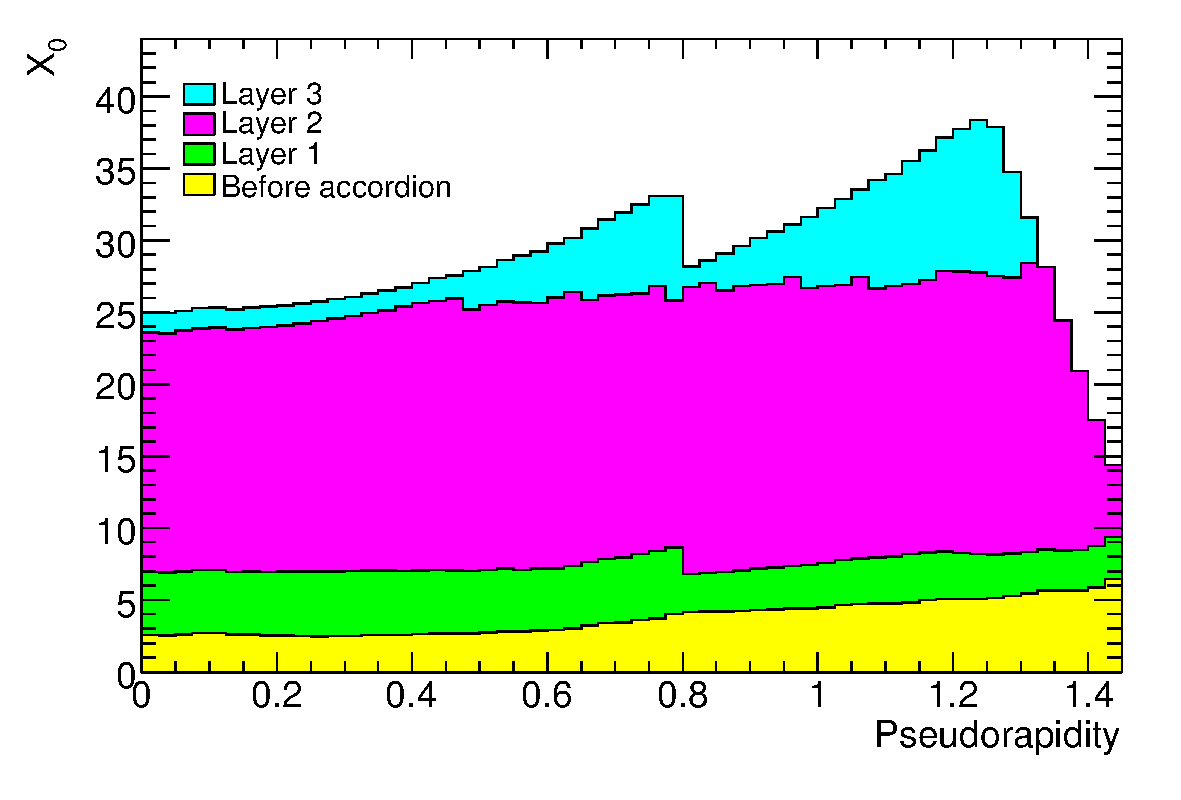
\includegraphics[width=0.46\textwidth]{PartDetector/Plots/x0_layers_barrel_csc03.pdf}
  ~
  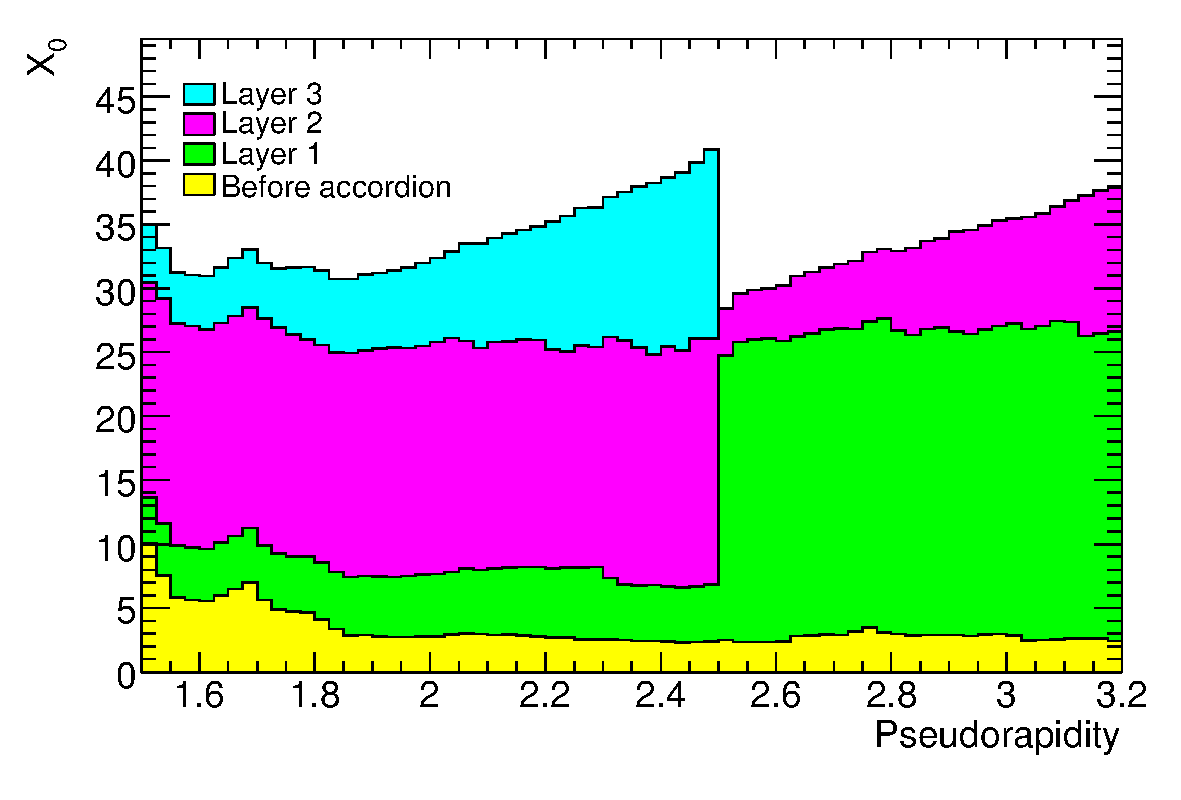
\includegraphics[width=0.46\textwidth]{PartDetector/Plots/x0_layers_endcap_csc03.pdf}
  \caption[Cumulative amounts of material, in units of radiation length $X_{0}$, as a function of $|\eta|$ in front and in the EM calorimeter at the ATLAS detector.]{Cumulative amounts of material, in units of radiation length $X_{0}$, as a function of $|\eta|$ in front and in the EM calorimeter at the ATLAS detector~\cite{Detector:ExpectedPerf}. The left-hand plot shows the amount of material in the barrel region and the right-hand plot shows the material in the endcap region.}
  \label{fig:DetectorInteraction}
\end{figure}

In the region devoted to precision physics the EM calorimeter is divided into three segments as shown in Figure~\ref{fig:DetectorECalSegment}, the strip layer is designed to improve particle identification and pseudorapidity measurement. The design energy resolution for all components of the calorimeter are shown in Table~\ref{tab:DetectorCaloResolution}.

\begin{table}[htb]
  \ra{1.3}
  \centering
  \begin{tabular}{@{}ll@{}}
    \toprule
    Section   & Resolution \\
    \midrule
    EM Barrel & $\frac{10\%}{\sqrt{E}}\oplus0.7\%$ \\
    EMEC      & $\frac{10\%}{\sqrt{E}}\oplus0.7\%$ \\
    HEC       & $\frac{100\%}{\sqrt{E}}\oplus10\%$ \\
    FCAL      & $\frac{100\%}{\sqrt{E}}\oplus10\%$ \\
    % EM Barrel & $\frac{10.1\%}{\sqrt{E}}\oplus0.17\%$~\cite{Energy} \\
    % HEC       & $\frac{70.6\%}{\sqrt{E}}\oplus5.8\%$ \\ MEASURED
    % FCAL      & $\frac{95\%}{\sqrt{E}}\oplus7.5\%$~\cite{Detector:FCalMeasuredPerf} \\ MEASURED
    \bottomrule
  \end{tabular}
  \caption[Design energy resolution of all ATLAS calorimeter components.]{Design energy resolution of all ATLAS calorimeter components~\cite{Detector:ATLASExperimentGeneral}. The resolution is made of a sampling term ($\nicefrac{1}{\sqrt{E}}$) associated with the choice of passive and active materials and the construction of the layers, and a constant term associated with the depth of the detector, cracks and dead material.} \label{tab:DetectorCaloResolution}
\end{table}

\begin{figure}[htbp]
   \centering
   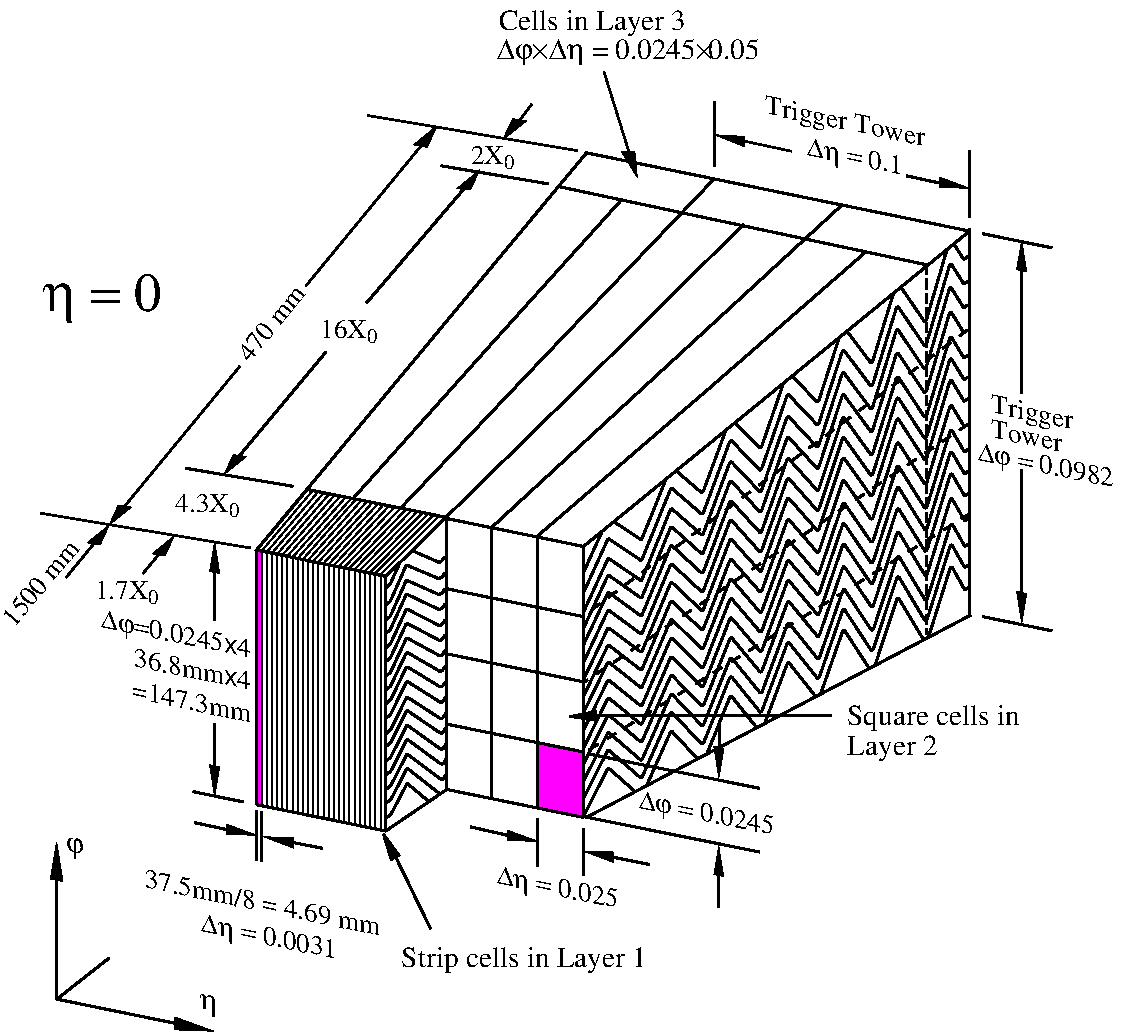
\includegraphics[width=0.75\textwidth]{PartDetector/Diagrams/LARG3-TDR-barrelM.pdf}
   \caption[Cut-away diagram of the EM calorimeter barrel at $\eta=0$.]{Cut-away diagram of the EM calorimeter barrel at $\eta=0$~\cite{Detector:ATLASExperimentGeneral}. Shown are the three different layers with varying cell structures. The strip section is designed to enhance particle identification and position measurement in $\eta$.}
   \label{fig:DetectorECalSegment}
 \end{figure} 

\subsubsection{Hadronic calorimeter}
The hadronic calorimeter uses different types of passive and active material to accommodate for the varying conditions in different regions of the detector. The structure of the detector and the materials used must provide good energy resolution, full symmetric coverage for the purpose of \met\ measurement, full containment of all hadronic activity to prevent punch-through to the muon system, and be sufficiently radiation hard. The hadronic calorimeter consists of two parts: a scintillator tile calorimeter in the barrel region and a LAr calorimeter in the end-cap.

The tile calorimeter is located directly outside the EM calorimeter. The barrel portion covers $\aeta<1.0$ and the two extended barrels cover the range $0.8<\aeta<1.7$. The tile calorimeter uses steel as the passive material and scintillating tiles as the active material. The resulting hadronic showers enter the scintillating tiles and produce photons which are passed to photomultiplier tubes. The total detector thickness which is tile-instrumented is $9.7\lambda_{\textrm{int}}$ at $\eta=0$.

The hadronic end-cap (HEC) uses LAr technology due to its radiation-hardness in this challenging high pseudorapidity region. The HEC consists of two independent wheels per end-cap covering the range $1.5<\aeta<3.2$ overlapping the tile calorimeter at low pseudorapidity and the forward calorimeter located at high pseudorapidity.

\subsubsection{Forward calorimeter}

The forward calorimeter (FCal) is responsible for energy measurement in the very high pseudorapidity range $3.1<\aeta<4.9$ of both electromagnetic and hadronic activity. Due to the large amount of radiation in this region, LAr is employed as the active material. The FCal consists of three layers: the first made primarily of copper, designed mostly for the measurement of electromagnetic activity, while the two outer tungsten layers are responsible for hadronic activity measurement.

\subsection{Muon spectrometer}

The muon spectrometer (MS) is the outermost layer of the ATLAS detector (Figure~\ref{fig:DetectorDrawingMuonSystem}) and is responsible for the precision measurement of \pt\ of charged-particles that pass-through the ATLAS calorimetry. It is designed to have a precision of \SI{10}{\percent} at a momentum of \SI{1}{\TeV}~\cite{Detector:ATLASExperimentGeneral}. Muon tracking performance is vital to the SMT tagger described in Section~\ref{sec:DetectorSLT}, as it relies on the precise reconstruction of muon tracks in the ID and MS.

Due to their larger mass, muons tend to have a larger transverse momentum and do not lose as much energy through photon emission. As a result, muons tend to traverse the hadronic calorimeter and escape the detector volume. The muon system provides measurement of these particles up to $\aeta<2.7$ and triggering up to $\aeta<2.4$. Measurement of \pt\ is facilitated by the magnetic field generated by the large toroid magnet in the barrel region $\aeta<1.4$ and two smaller end-cap magnets in $1.6<\aeta<2.7$. In the transition region at $1.4<\aeta<1.6$, deflection is provided by both barrel and end-cap fields. 

\begin{figure}[p]
  \centering  
  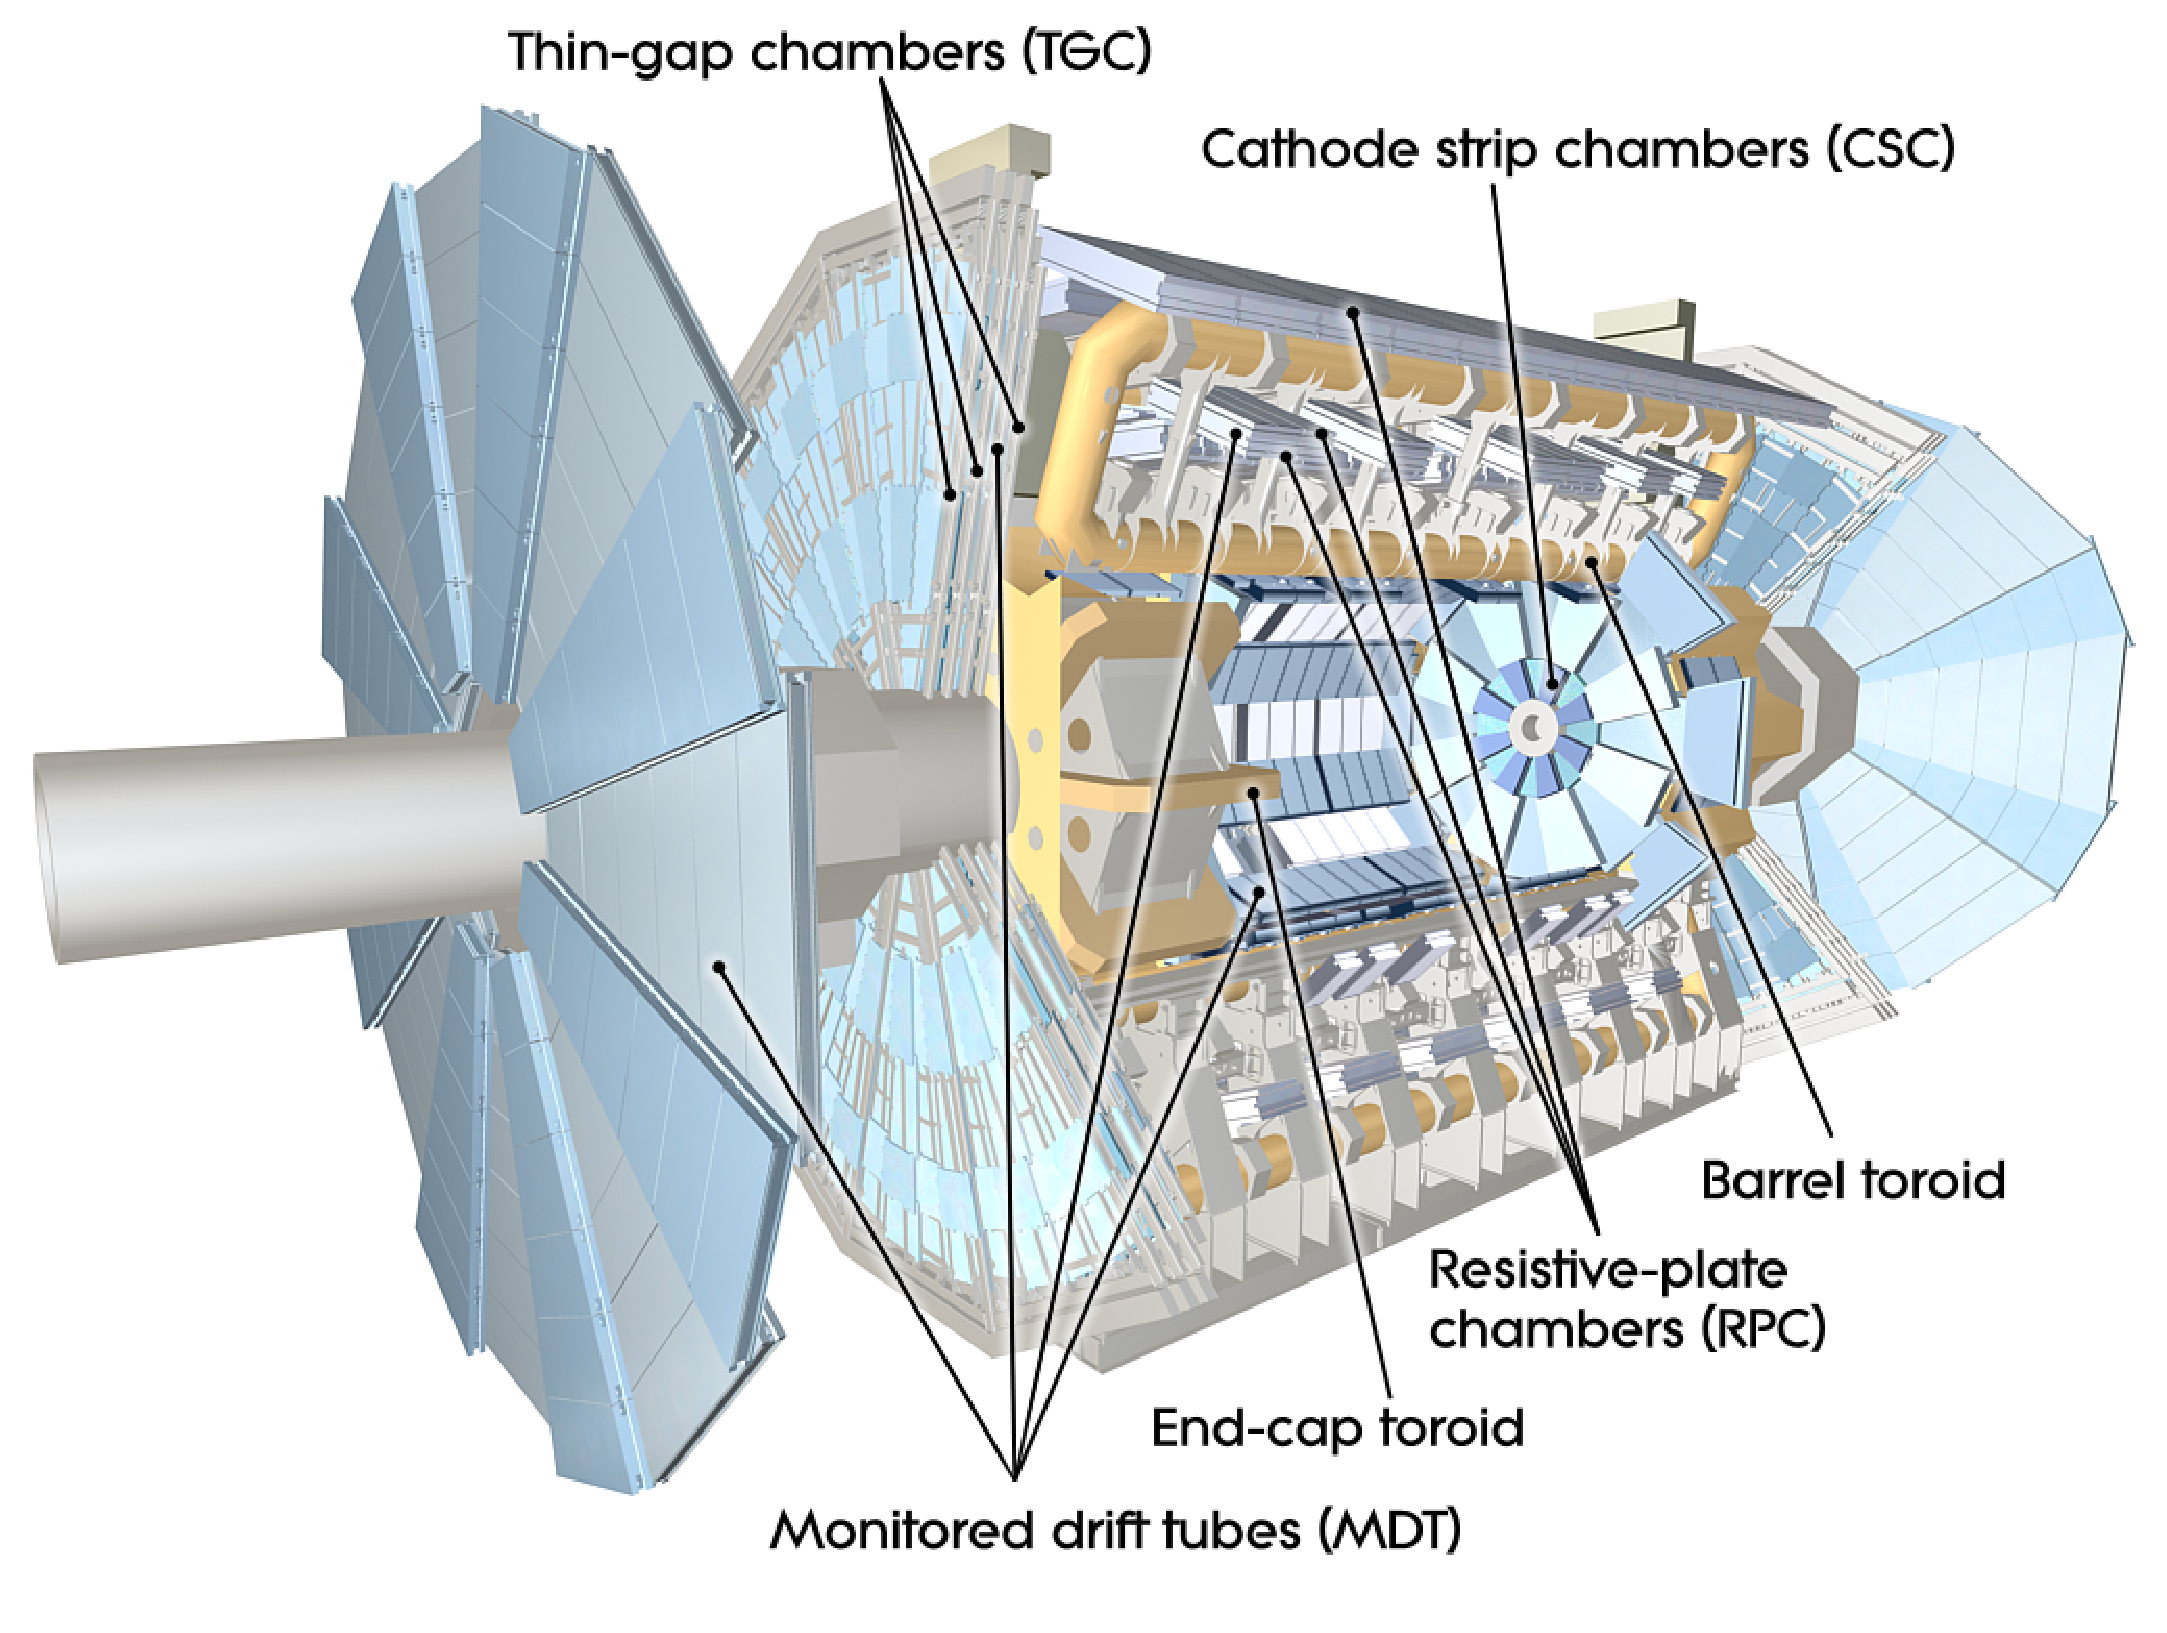
\includegraphics[width=0.80\textwidth]{PartDetector/Diagrams/ATLAS_MuonSystem.eps}
  \caption[Cut-away drawing of the ATLAS muon system.]{Cut-away drawing of the ATLAS muon system~\cite{Detector:ATLASExperimentGeneral}.}
  \label{fig:DetectorDrawingMuonSystem}
\end{figure}

The structure of the MS is delimited by the magnet system. In the barrel region, three cylindrical layers of precision-tracking chambers are located in and on the coils of the barrel toroid magnet at radii of ~\SIlist{5;7.5;10}{\meter}. End-cap region coverage is provided by three chamber planes perpendicular to the $z$-axis. These are located in front and behind the end-cap toroid magnet at distances $|z|\approx$~\SIlist{7.4;10.8;14;21.5}{\meter} from the interaction point.

The MS contains four different types of chambers responsible for precision-tracking and/or triggering in various pseudorapidity ranges, as shown in Table~\ref{tab:DetectorMSOverview}. The arrangement of these chambers is shown in Figure~\ref{fig:DetectorMuonOverview}.

\begin{table}[htb]
  \centering
  \begin{tabular}{@{}ll@{}}
    \toprule
    \textbf{Monitored drift tubes} & \textbf{MDT} \\
    \midrule
    - Coverage                     & $\aeta<2.7$ (innermost layer: $\aeta<2.0$) \\
    - Number of chambers           & 1150 \\
    - Function                     & Precision tracking \\
    \bottomrule
    \textbf{Cathode strip chambers} & \textbf{CSC} \\
    \midrule
    - Coverage                      & $2.0<\aeta<2.7$ \\
    - Number of chambers            & 32 \\
    - Function                      & Precision tracking \\
    \bottomrule
    \textbf{Resistive place chambers} & \textbf{RPC} \\
    \midrule
    - Coverage                        & $\aeta<1.05$ \\
    - Number of chambers              & 606 \\ 
    - Function                        & Triggering, second coordinate \\
    \bottomrule
    \textbf{Thin gap chambers}        & \textbf{TGC} \\
    \midrule
    - Coverage                        & $1.05<\aeta<2.7$~(2.4 for triggering) \\
    - Number of chambers              & 3588 \\
    - Function                        & Triggering, second coordinate \\
    \bottomrule
  \end{tabular}
  \caption[Main parameters of the muon system.]{Main parameters of the muon system~\cite{Detector:ATLASExperimentGeneral}.}
  \label{tab:DetectorMSOverview}
\end{table}

\begin{figure}[tbhp]
  \centering
    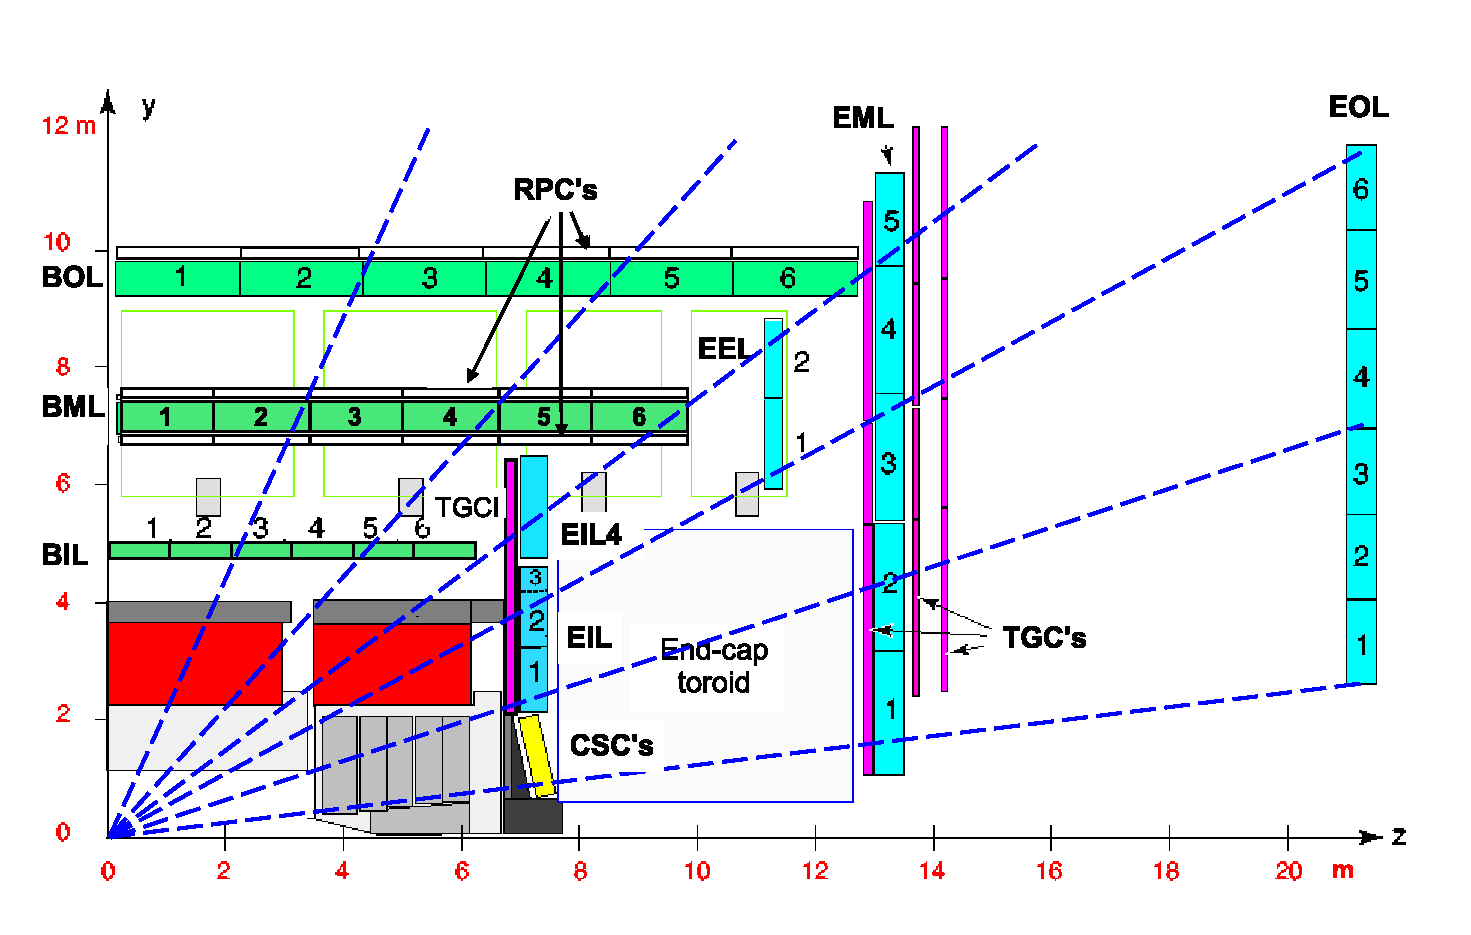
\includegraphics[width=0.80\textwidth]{PartDetector/Diagrams/Muon_section.eps}
    \caption[Plan view of quarter-section of the ATLAS muon spectrometer.]{Plan view of quarter-section of the ATLAS muon spectrometer~\cite{Detector:ATLASExperimentGeneral}.}
  \label{fig:DetectorMuonOverview}
\end{figure}

\begin{figure}[htbp]
  \centering
    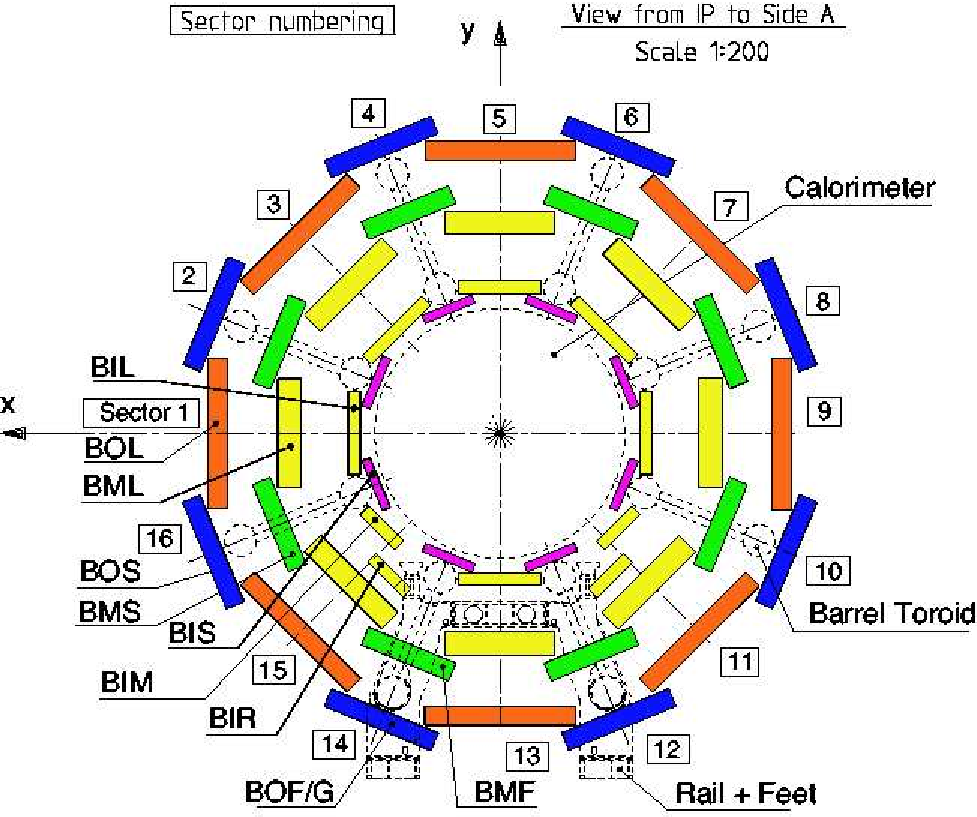
\includegraphics[width=0.80\textwidth]{PartDetector/Diagrams/Muon_sector_numbering.pdf}
    \caption[Transverse view of the muon system.]{Transverse view of the muon system~\cite{Detector:ATLASExperimentGeneral}.}
  \label{fig:DetectorTransverse}
\end{figure}

In the barrel region, precision-measurement is performed by monitored drift tube (MDT) chambers. These chambers consist of three to eight pressurized aluminium drift tubes, each containing a tungsten-rhenium wire anode and a mixture of argon and carbon dioxide gas. An average spatial resolution of \SI{80}{\um} per tube and \SI{35}{\um} per chamber is achieved.

The end-cap region is instrumented with cathode-strip chambers (CSC) due to their higher rate capability and time resolution. CSCs are multi-wire chambers with cathode planes segmented into strips in orthogonal directions, this allows both coordinates to be measured simultaneously. The resolution of a chamber is \SI{40}{\um} in the bending plane ($R$-$z$) and \SI{5}{\mm} in the transverse plane.

Triggering on muon tracks is another essential role of the muon spectrometer. To this end, each precision-measurement chamber is complemented with fast triggering chambers. As with the measurement layers, two different types of chambers are used for the barrel and end-cap regions. In the barrel region ($|\eta<1.05$), resistive plate chambers (RPC) are attached to the same support structure as the MDTs. The RPCs are made of two resistive plates, \SI{2}{\mm} apart, between which a potential difference is applied. The gap between the plates is filled with a mixture of $\textrm{C}_2\textrm{H}_2\textrm{F}_4$/Iso-$\textrm{C}_4\textrm{H}_{10}$/$\textrm{SF}_6$. The signal is read out via metallic strips mounted to the outer faces of the resistive plates. The end-cap region ($1.05<\aeta<2.4$) is populated with thin gap chambers (TGC). TGCs are multi-wire chambers like those used in the CSC, however the distance between the wire and the cathode is smaller in the TGC. A summary of the spatial and temporal resolution for the measurement and triggering layers is shown in Table~\ref{tab:MSPerfomanceSummary}.
%
\begin{table}[htb]
  \centering
  \sisetup{range-phrase=-,range-units=single}
  \begin{tabular}{@{}lccc@{}}
   \toprule
   Chamber & \multicolumn{3}{c}{Resolution in} \\
   \cmidrule{2-4}
           & $R/z$ & $\phi$ & Time \\
   \midrule
   MDT & \SI{35}{\um} $(z)$        & --                  & --            \\
   CSC & \SI{40}{\um} $(R)$        & \SI{5}{\mm}         & \SI{7}{\ns}   \\
   RPC & \SI{10}{\mm} $(z)$        & \SI{10}{\mm}        & \SI{1.5}{\ns} \\ 
   TGC & \SIrange{2}{6}{\mm} $(R)$ & \SIrange{3}{7}{\mm} & \SI{4}{\ns}   \\
   \bottomrule
  \end{tabular}
  \caption[Summary of spatial and temporal resolutions per chamber for all chamber types used in the ATLAS muon spectrometer.]{Summary of spatial and temporal resolutions per chamber for all chamber types used in the ATLAS muon spectrometer. Adapted from~\cite{Detector:ATLASExperimentGeneral}.}
  \label{tab:MSPerfomanceSummary}
\end{table}

\subsection{Magnet system}
The structure of the ATLAS detector is defined by its large magnet systems as shown in Figure~\ref{fig:DetectorMagnet}. The system consists of two sets of magnets: the CS and three air-core toroids.

The CS is located nearest to the beam and provides a \SI{2}{\tesla} magnetic field for the ID for the purpose of tracking, particle identification and \pt\ measurement.

The barrel toroids extend to $\aeta<1.4$ and are made of eight coils, generating a \SI{0.5}{\tesla} magnetic field for the MS. In the high pseudorapidity range, magnetic deflection is provided by two end-cap toroids extending from $1.6<\aeta<2.4$. As in the barrel, the end-cap toroids are made of eight coils offset by \SI{22.5}{\degree} with respect to the barrel coils. Each end-cap generates a \SI{1}{\tesla} magnetic field for the MS. The so-called transition region between the two magnets is covered by the overlap of the end-cap and barrel fields.

\begin{figure}[htbp]
  \centering
  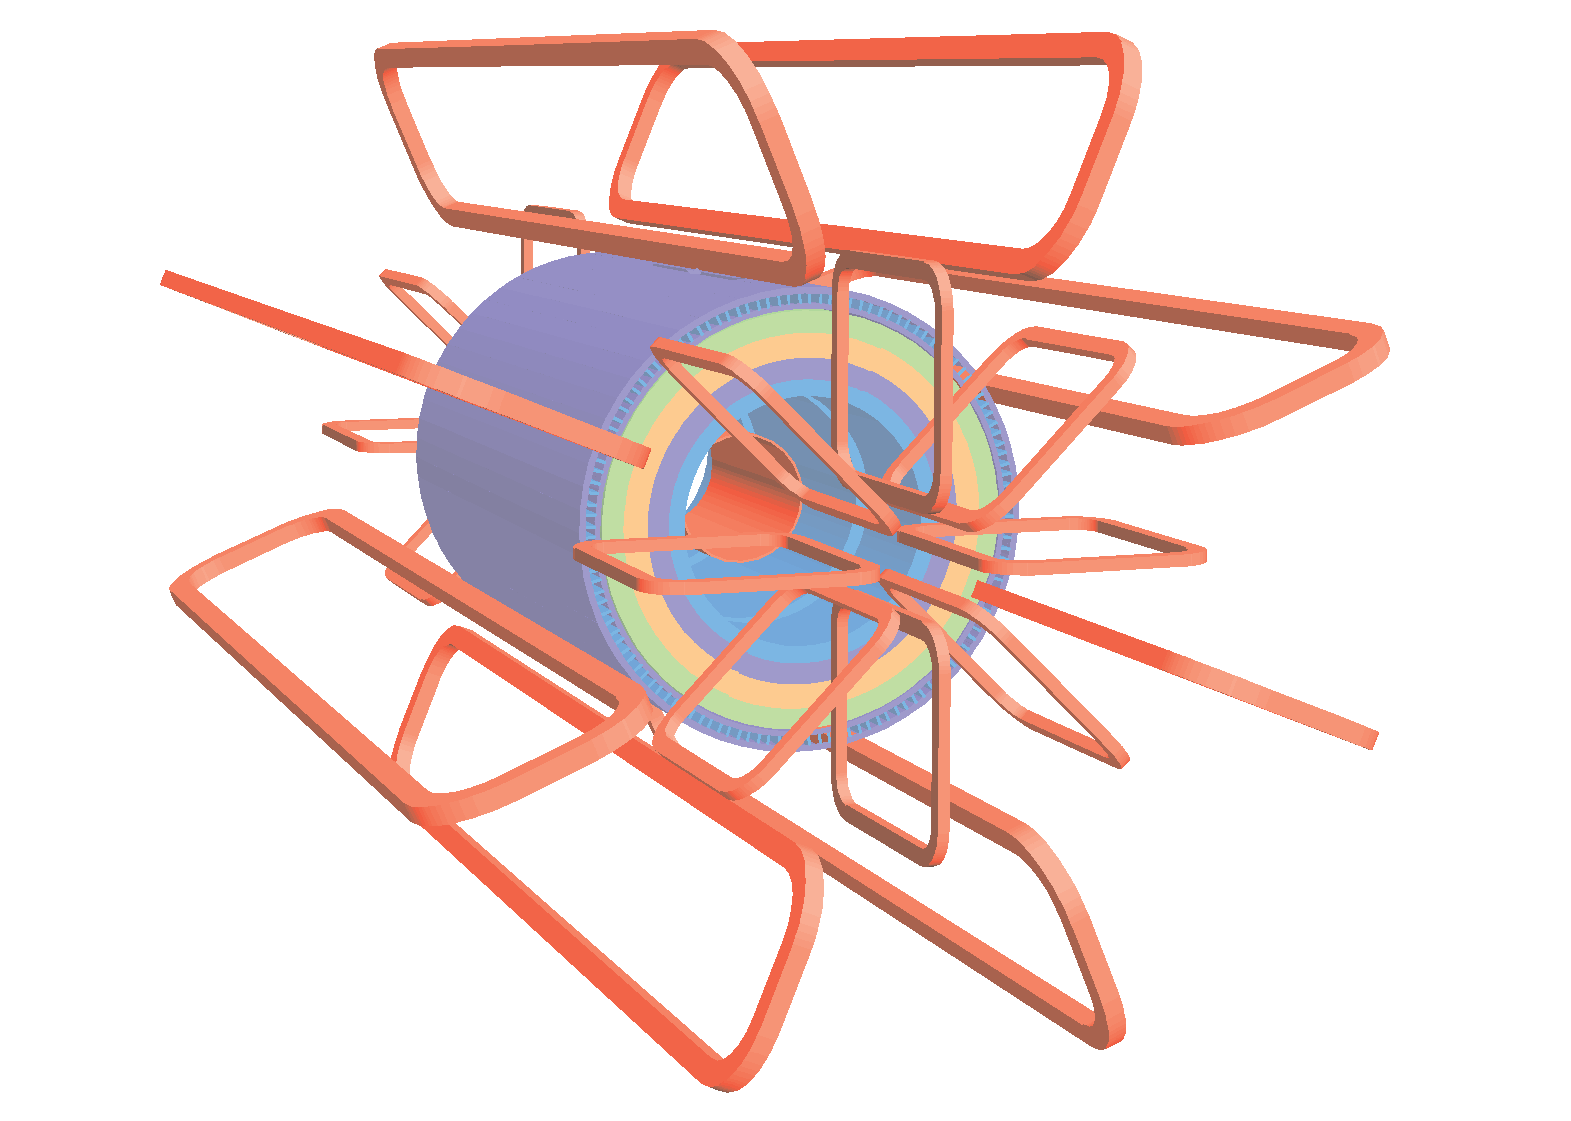
\includegraphics[width=0.80\textwidth]{PartDetector/Diagrams/ATLcoilGeom.eps}
  \caption[Diagram of the ATLAS toroid magnet system.]{Diagram of the ATLAS toroid magnet system~\cite{Detector:ATLASExperimentGeneral}. The red central solenoid is located closest to the beam surrounded by layers of tile calorimetry. The eight barrel toroid magnets are shown along with the offset end-cap toroids at each end.}
  \label{fig:DetectorMagnet}
\end{figure}

\subsection{Beam-pipe}

The beam-pipe section located within the ATLAS experiment is approximately \SI{38}{\meter} in length and made of seven parts. The central chamber has an inner diameter of \SI{58}{\mm} and is constructed from \SI{0.8}{\mm} thick beryllium due to the material's transparency to particles, high specific stiffness and compatibility with ultra-high vacuum. The beam-pipe is centred around the IP and integrated with the pixel detector. The additional layers are made of stainless steel located symmetrically on both sides of the IP.

\subsection{Triggering and data-acquisition}

At the design luminosity of the LHC $\Lagr=\SI{10e34}{\per\square\cm\per\second}$, the expected event rate is approximately \SI{1}{\GHz}. At an average event size of \SI{1.3}{\mega\byte} per event, the total amount of data produced at ATLAS is \SI{1.2}{\peta\byte\per\second}. The maximum rate of data storage at ATLAS is approximately \SI{300}{\mega\byte\per\second}, so the rate must be reduced.

The trigger and data acquisition system (TDAQ) is responsible for reducing the rate by recording only ``interesting'' events. This is known as \emph{online selection} as it happens before the data is stored. In contrast, \emph{offline selection} happens after the data has been recorded, for example when performing a cross section measurement. The overwhelming majority of events produced at the LHC are of no interest to physics analysis, for example the so-called \emph{minimum bias events}. 

At ATLAS, trigger decisions are carried out in three sequential levels: \emph{Level 1} (L1), \emph{Level 2} (L2) and \emph{Event Filer} (EF), each successive level reduces the rate by applying more complex selection criteria. The hardware-based L1 trigger, performs the initial selection based on reduced-granularity information from the MS trigger chambers and all calorimeters. Data from the calorimeter trigger towers, shown in Figure~\ref{fig:DetectorECalSegment}, is used to search for high transverse-momentum muons, photons, electrons, hadronic decays of $\tau$ leptons, hadronic jets, large missing transverse energy, and large total transverse energy. The central trigger processor applies the trigger `menu' which includes a combination of selection criteria. Events which are of interest to physics analyses can be produced at such a rate as to overwhelm the capabilities of the DAQ. A \emph{prescale} can be applied to record one out of many of these events, thus reducing the rate. The L1 trigger also constructs \emph{regions of interest} (RoIs) around the detector where interesting features have been found. The $\eta$ and $\phi$ information of the RoI along with information about the decision is stored and passed to the higher level triggers.

The L2 selection makes use of RoIs and the full granularity of the detector to further reduce the event rate to approximately \SI{3.5}{\kHz}, and finally the EF implements selections commonly used for offline analysis to reduce the rate to \SI{200}{\Hz}.

\section{Monte carlo simulation} \label{DetectorMC}

The simulation of data is paramount to HEP research, from the initial detector design phase all the way through to finalized analyses. Monte Carlo (MC) generators simulate various interactions, creating kinematic collision event data that reflect our best understanding of nature. These processes are then passed through detector simulation and all the object reconstruction algorithms, resulting in a dataset with an identical format to collision data. More information on the ATLAS simulation infrastructure can be found in~\cite{Detector:ATLASSimulationInfra}.

The simulation of data happens in three phases: event generation, detector simulation and digitization. 

\subsection{Event generation} \label{DetectorEventGeneration}

Event generators model complex physics processes that occur during a particle collision. Many different generators exist to model a variety of beam types ($pp$, $p\bar{p}$, $e^+e^-$, etc\ldots) and event types. Hadronic event generators simulate all components of the interaction: the hard scattering process, parton showering, hadronizing, hadronic decay, the underlying event, and photon radiation~\cite{Les}. A schematic diagram of a hadronic event as modelled by an event generator is shown in Figure~\ref{fig:DetectorEGSketch}.

\begin{figure}[p]
  \centering
  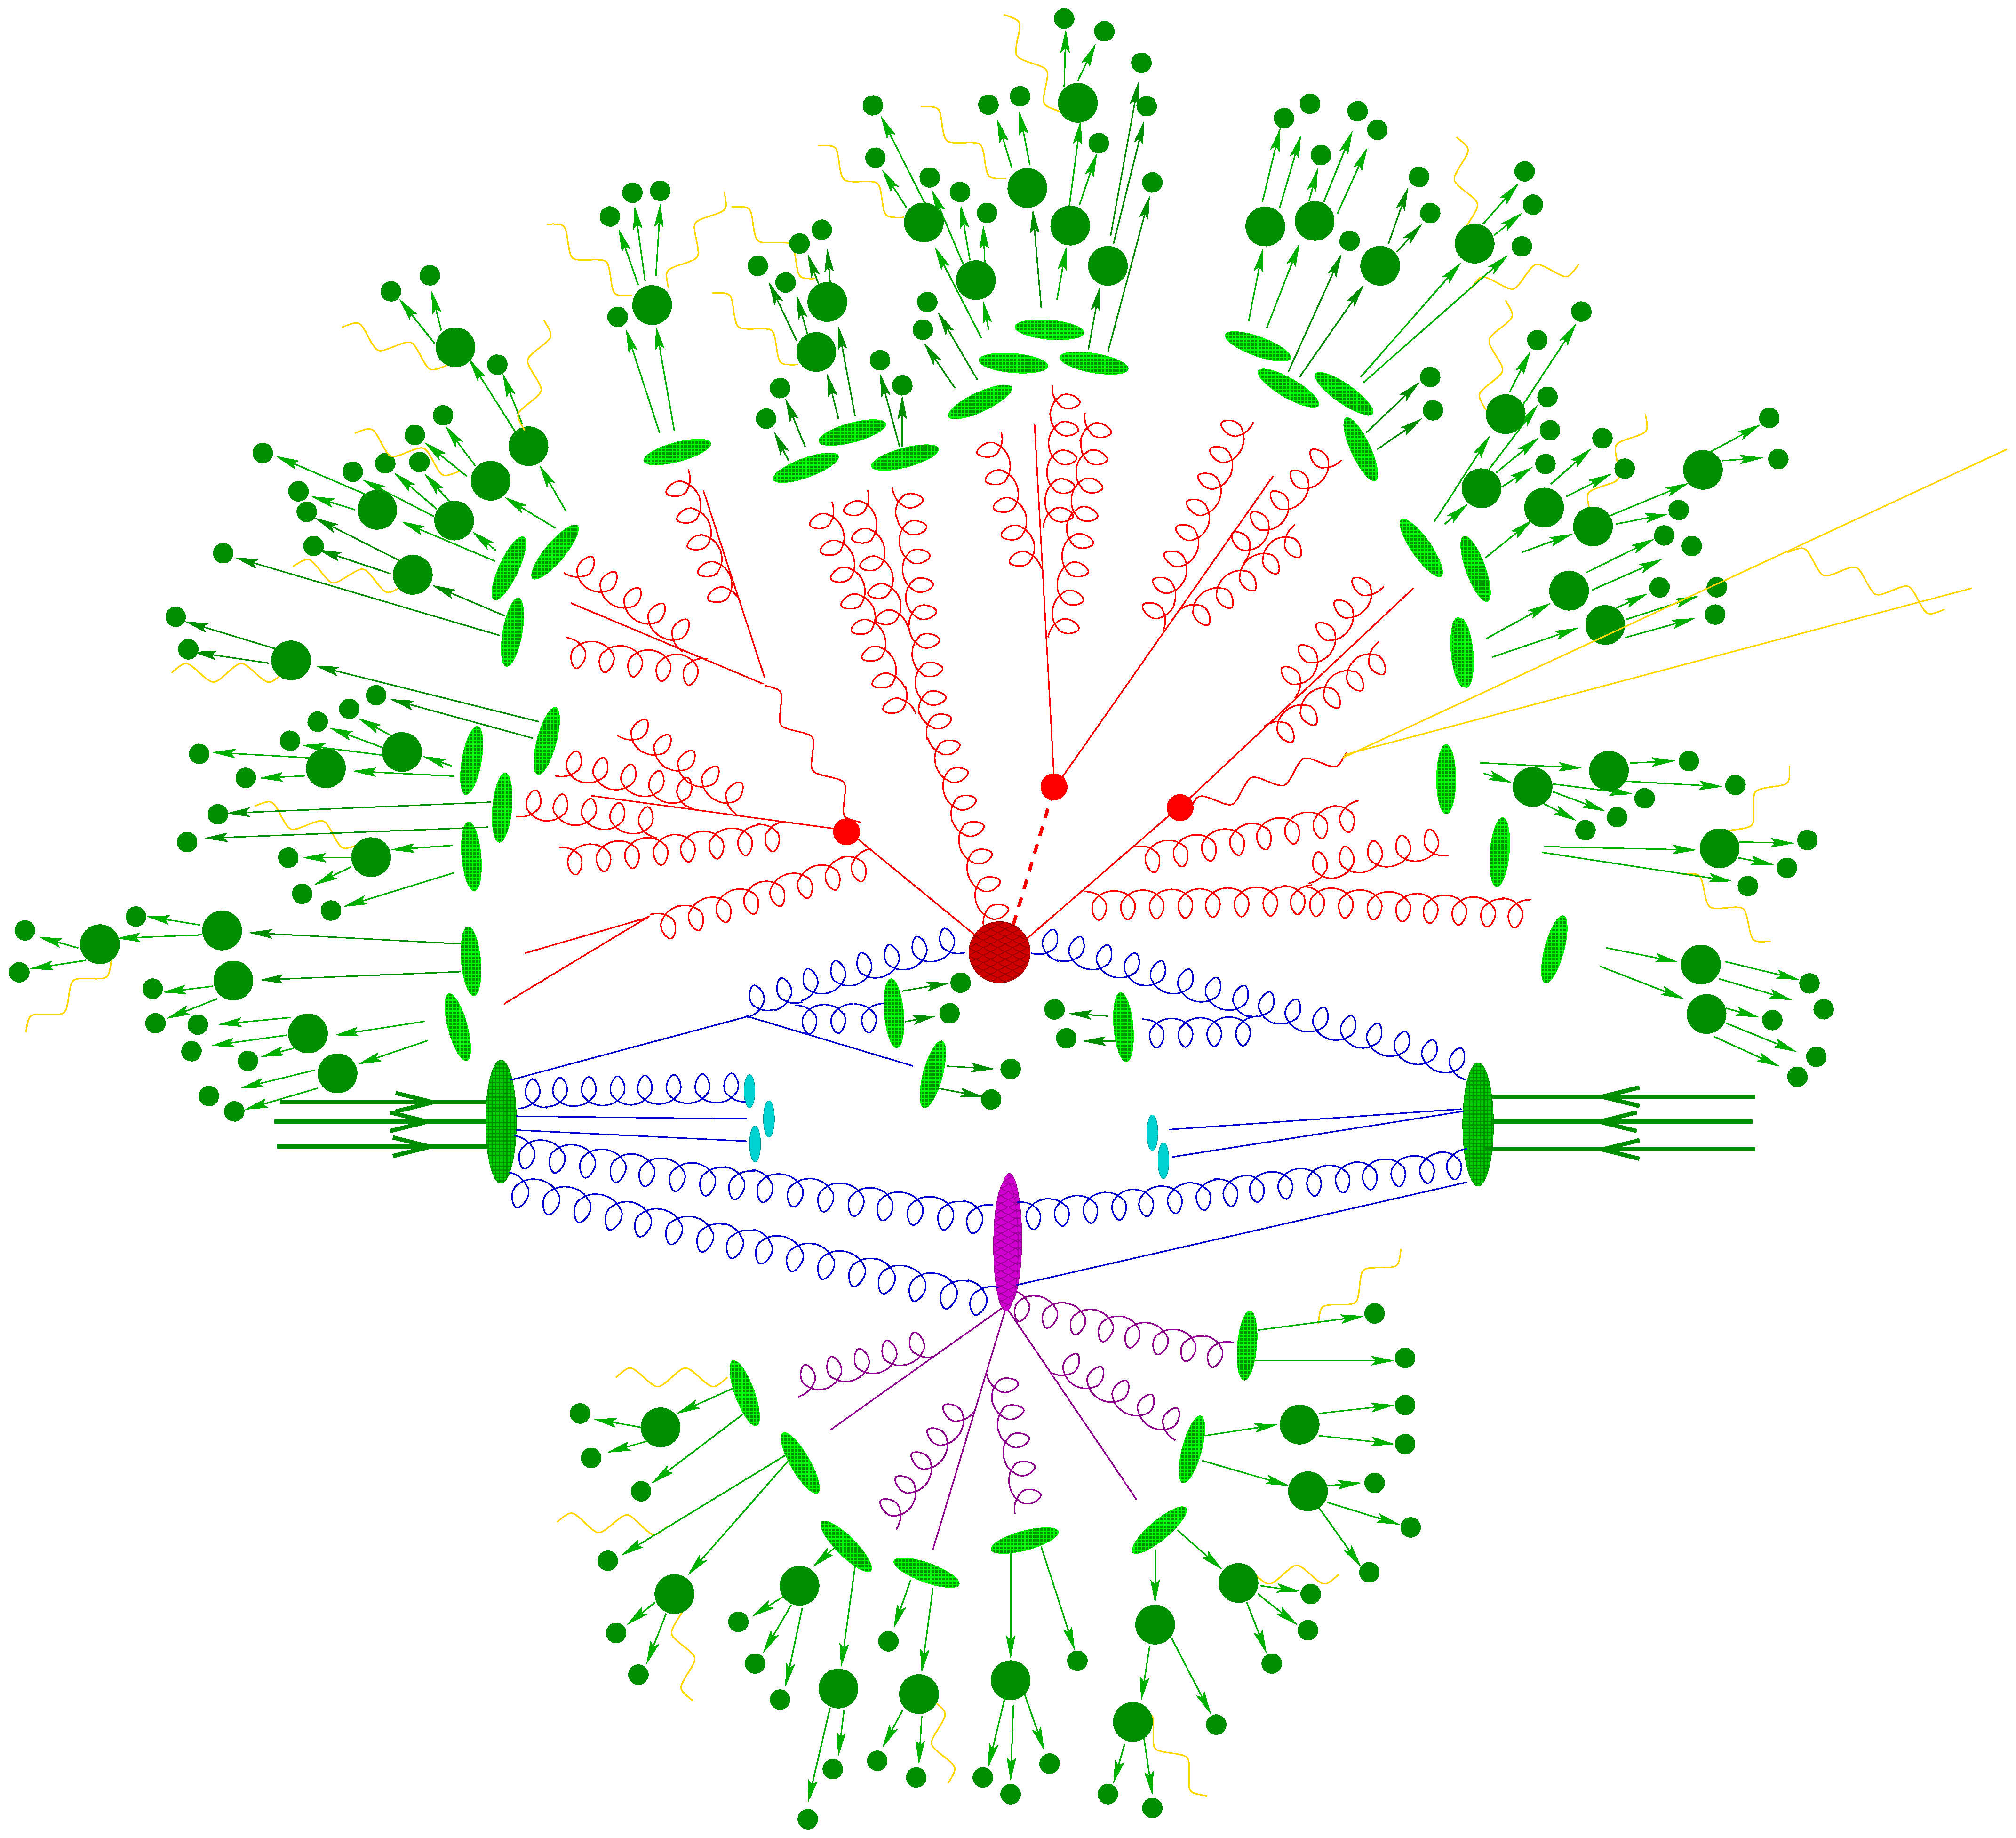
\includegraphics[width=0.90\textwidth]{PartDetector/Diagrams/scetch.eps}
  \caption[Sketch of a proton-proton collision as modelled by the event generator.]{Sketch of a proton-proton collision as modelled by the event generator~\cite{Event}. Shown are the incoming protons beams as green arrows on the left and right sides of the diagram. The partons shown in blue, interact in the hard interaction (red blob) producing a parton shower, also depicted in red, which eventually hadronize (light green blobs) and finally decay into final state particles shown in dark green. The \emph{underlying event} is shown at the bottom of the diagram as the purple blob, note also the beam remnants as light blue blobs that also form part of the underlying event. Photon emission is shown in yellow and occurs at all stages of the event generation.}
  \label{fig:DetectorEGSketch}
\end{figure}

First, the \emph{hard interaction} of a pair of partons originating from the colliding protons is simulated. An example of such an interaction is $q\bar{q} \rightarrow Z / \gamma^{*}\rightarrow e^{+}e^{-}$. Calculating the cross section for such an interaction involves the convolution of the parton density function (PDF) and the \emph{matrix element} (ME).

The PDF $f_i(x,Q^2)$, describes the probability of finding, within the proton, a parton of flavour $i$ carrying a fraction $x$ of the proton momentum, via a hard interaction with energy scale $Q$. The ME describes the interaction between the two partons and corresponds to one or more of the Feynman diagrams associated with the interaction\footnote{For a rigorous discussion of matrix elements and the Feynman rules, see~\cite{Theory:Perkins,Theory:IntroGriffiths}}. The order of a diagram is determined by the number of coupling constants associated with it. Different generators are capable of treating diagrams at different orders, though the hard interaction is usually modelled at LO or NLO.

The next step is \emph{parton-showering} which simulates the emission of gluons by coloured partons. A cascade of partons is produced, as shown in Figure~\ref{fig:DetectorEGSketch}, and modelled by perturbation theory for energies above \SI{1}{GeV}. All coloured objects are then combined into colourless hadrons in a process known as \emph{hadronization}, these hadrons are subsequently allowed to decay. Finally, the remaining coloured partons not involved in the hard interaction, are allowed to interact forming the \emph{underlying event}. The kinematic information of the original event without the effects of the detector is kept in the data set and is usually referred to as the \emph{truth information}.

\subsection{Detector simulation} \label{sec:DetectorSimulation}

The generated events are then passed through a detector simulation that mimics the response of the detector to particles traversing through it. A description of the entire detector is implemented in the GEANT4 tool-kit~\cite{Detector:Geant4}, including a map of the magnetic fields, the position of the detector components and material description. The software then simulates the signal voltages produced in all tracking and calorimeter components of the detector, these are then passed through a simulation of the read-out electronics and TDAQ taking into account known losses and inefficiencies. All of this information is then passed on to the reconstruction software that ``rebuilds'' the physics objects from the detector hits.

\section{Object reconstruction} \label{sec:DetectorEventReco}

The process of converting the raw data from the detector into physics objects (electrons, muons and so on) is known as \emph{object reconstruction}. The reconstruction algorithms are identical for both collision data and simulated data. As lepton plus jets decays of \ttbar\ are the focus of this thesis, the reconstruction procedures of all types of objects (excluding photons) are relevant. This includes electron, muon and jet reconstruction as well as $b$-tagging algorithms. The soft muon tagger relies on \emph{STACO combined} muons, therefore some details of the muon reconstruction algorithms are discussed here.

\subsection{Electron reconstruction} \label{sec:DetectorElReco}

The electron reconstruction~\cite{Detector:ElectronReco} procedure at ATLAS depends on the pseudorapidity of the candidate. Only electrons that lie within the coverage of the ID are used here, therefore only the relevant procedure is described. The algorithm used in the central region identifies energy deposits in the EM calorimeter and associates them with reconstructed ID tracks. Firstly, clusters are seeded from energy deposits with total \Et\ above \SI{2.5}{\GeV} using a sliding-window algorithm with window size $3\times5$ in units of $0.025\times0.025$ in ($\eta$,$\phi$) space. Tracks with $\pt>\SI{0.5}{\GeV}$ are then extrapolated to the middle layer of the EM calorimeter and matched to the cluster seed using cuts in the ($\eta$,$\phi$) space. In case of multiple matches, tracks with pixel or SCT hits are given priority and the match with the smallest \DeltaR\ distance is chosen. Finally, the size of the cluster associated with the candidate electron is enlarged to $3\times7$ and $5\times5$ in the barrel and end-cap regions respectively. The energy of the electron is then the sum of four contributions taking into account energy deposited before the EM material, and leakages to other clusters as well as beyond the EM calorimeter.

Electron identification for central electron candidates is done by applying sequential cuts on calorimeter, tracking and combined track-cluster variables. Several sets of selection criteria, labelled \emph{loose}, \emph{medium} and \emph{tight}, are designed for use in analyses. These sets provide increasing background-rejection power at the cost of efficiency by introducing new cuts at each stage, or by tightening previous cuts. The cut definitions are listed in Appendix~\ref{app:DetectorElectronID}.

Additional requirements can be made on the so-called isolation of the electron. Three sets of isolation strategies are used at ATLAS~\cite{Detector:ElectroIsolation}:

\begin{itemize}
  \item \textbf{Calorimeter isolation}: The calorimeter isolation \etcone{\DeltaR}\ is defined as the sum of transverse energy deposited in the cells around the electron in a cone of size \DeltaR. The contribution from the electron itself is removed within $\Delta\eta\times\Delta\phi=0.125\times0.175$ around the electron cluster barycentre. It is corrected for energy leakage from the electron into the isolation cone and for the effect of pile-up. At ATLAS the nominal cone sizes used are $\DeltaR$=\numlist{0.2;0.3;0.4}.
  \item \textbf{Track isolation}: The tracking isolation \nucone{\DeltaR}\ is defined as the number of tracks in a cone around the electron, excluding the track of the electron itself.
  \item \textbf{Momentum isolation}: The momentum isolation \ptcone{\DeltaR}\ is defined by the sum of the transverse momentum of tracks with $\pt>\SI{0.4}{\GeV}$ in a cone around the electron, excluding the electron track itself.
\end{itemize}

\subsection{Muon reconstruction} \label{sec:DetectorMuReco}

Muon reconstruction makes use of the information provided by both the inner detector and the muon spectrometer systems. Several different strategies exist~\cite{Detector:MuonReconstructionList}:

\begin{itemize}
  \item \textbf{Standalone reconstruction}: Uses MS information only, first constructing \emph{segments} from several hits in a given chamber and then fitting segments from all three stations to hits from the four MS components. Tracks are then extrapolated back to the interaction point taking into account energy loss and multiple scattering.
  \item \textbf{Tagging ID tracks reconstruction}: Uses MS or calorimeter information to tag ID tracks as muons.
  \item \textbf{Combined track reconstruction}: Standalone muon tracks are extrapolated back to the vertex and matched to ID tracks within ($\aeta<2.5$) and combined. This results in an improved momentum sensitivity from ID and MS information. 
\end{itemize}

These strategies can be implemented in a variety of ways. There are two prominent families, STACO and MUID, that contain reconstruction packages which exploit one or a combination of these strategies. The STACO combined algorithm is used by the SMT tagger and is described in more detailed below.

\subsubsection{STACO Combined algorithm} \label{sec:DetectorSTACO}
The STACO package~\cite{Detector:STACO} combines ID and MS tracks by performing a statistical combination of the two independent tracks using track parameters ($\eta$, $\phi$, \pt, $d_{0}$, and $z_{0}$) and their covariance matrices. The quality of the fit is represented in the resulting \xsm:
%
\begin{equation}
  \xsm = (\Tms-\Tid)^T(\Cms+\Cid)^{-1}(\Tms-\Tid)
  \label{eq:DetectorXsmDef}
\end{equation}
%
where \Tms\ and \Tid\ contain the track parameters for the MS track and the ID track respectively,
% 
\begin{equation}
  \T_{\textrm{MS or ID}} =
  \begin{pmatrix}
    \eta \\
    \phi \\
    \pt \\
    d_{0} \\
    z_{0}
  \end{pmatrix}
\end{equation}
%
and \Cms\ and \Cid\ are the covariance matrices, defined as
%
\begin{equation}
  \C_{ij} = (\T_i-\langle \T_i\rangle)(\T_j-\langle \T_j\rangle)
\end{equation}
%
where $\langle \T_i\rangle$ is the expectation value of $\T_i$. The full covariance matrix is shown in Appendix~\ref{app:DetectorCov}.

If more than one possible combination per track exists, the best combined \xsm\ is chosen and then the track is removed from the pool of tracks to be match. The algorithm continues making associations until no more tracks remain.

Finally, tracking, calorimeter and momentum isolation variables are defined in a similar way as with electrons.

\subsubsection{MUID algorithm} \label{sec:MUID}

The MUID reconstruction package~\cite{Detector:ExpectedPerf} implements all muon reconstruction strategies described before. The MUID standalone (SA) algorithm uses tracks and segments reconstructed at the muon spectrometer by the Moore algorithm~\cite{Detector:MooreReconstruction}, and extrapolates inwards to obtain track parameters at the vertex. The MuGirl algorithm searches for MS tracks and segments using an ID track as a seed. If the full track refit is successful a combined muon is made, otherwise a tagged muon is made. The MUID family also contains a combined muon algorithm that use a global fit of the tracks reconstructed in the ID and in the MS.

\subsection{Jet reconstruction} \label{sec:Detector-JetReconstruction}

As quarks and gluons hadronize and fragment they produce a large number of soft hadrons and high energy photons. A jet reconstruction algorithm attempts to recombine all these components to reconstruct the four-momentum vector of the original quark/gluon. This process results in an object known as a ``jet''. These jets are the closest physical representation of a hard quark or a gluon available to experimentalists. The development of jet reconstruction algorithms is driven by theoretical and experimental requirements. From a theoretical perspective, it is crucial that jet algorithms be \emph{infra-red and collinear} (IRC) safe. The probability of gluon emission approaches infinity in the collinear and soft regime. These infinities cancel out with virtual gluon emission. If jets resulting from hard particles are merged or split due to soft emission or collinear splitting these probabilities do not cancel and a divergence occurs. A jet algorithm is said to be IRC safe when the reconstructed jets remain unchanged under the addition of a soft emission or a collinear splitting. Jet algorithms should also be able to work given parton, hadron, or calorimeter information. From an experimental perspective, jet algorithms should be stable under increased luminosity or centre of mass energy, be computationally efficient and fast, and work independently of detector technology. 

There are many different jet reconstruction algorithms such as the Cambridge/Aachen, \kt\ and SISCone, however only the ATLAS default known as the anti-\kt\ algorithm is used here.

\subsubsection{Anti-\kt\ algorithm}

The anti-\kt\ algorithm is a clustering algorithm that sequentially combines objects to form cone-shaped jets~\cite{Cacciari:2008gp}. This algorithm has been found to be more resilient to the effects of pile-up and underlying event, and the shape of the jet is unaffected by soft radiation producing circular jets. It is also computationally efficient and fast given a smart implementation~\cite{Detector:FastJetKt}.

The clustering process begins by measuring two distances: the distance between all particles $d_{ij}$, and the distance between particle $i$ and the beam $d_{iB}$ defined as
%
\begin{align*}
    d_{ij} &= \textrm{min}(\kti^{-2}, \ktj^{-2})\frac{\Delta_{ij}^2}{R^{2}} \\
    d_{iB} &= \kti^{-2}
\end{align*}
%
where $\dij^2=(y_i-y_j)^2+(\phi_i-\phi_j)^2$, and \kti, $y_{i}$ and $\phi_{i}$ are the transverse momentum, rapidity, and azimuthal angle of object $i$. The parameter $R$ defines the characteristic cone size of the jet, note that by construction not all anti-\kt\ jets are conical. For every object both distances are calculated, if $d_{ij}$ is the smallest then objects $i$ and $j$ are combined forming proto-jets, if $q_{iB}$ is smallest the object is labelled as a final jet and removed from the list of objects to be combined. This process continues until all objects are removed. 

In general, soft particles will tend to combine with hard objects before combining with other soft objects. If two hard objects lie at $2R$ from each-other, they will both form conical shapes with radius $R$. Otherwise partially conical jets will form depending on the relative magnitudes of \kt\ of each particle. The standard value of $R$ used for ATLAS analyses is $0.4$, this is used here unless stated otherwise.

\subsubsection{Jet calibration}

The process of jet calibration corrects the jet energy as measured in the detector with the intention of recovering the energy of the original stable particle jet that entered the detector. Clusters of energy deposits in the calorimeter, known as topo-clusters, are constructed from topologically connected calorimeter cells~\cite{Detector:JetEnergyMeasurement}. Calorimeter jets are constructed from topo-clusters that enter the clustering algorithm as massless particles. 

These clusters are initially reconstructed at the EM scale, which correctly measures the energy of particles in EM showers. If jet reconstruction is carried on these clusters the jets are known as EM jets. An additional collection of topo-clusters is created by calibrating the calorimeter cells to correctly reconstruct the response of the calorimeter to hadrons. The main calibration scheme is known as \emph{local cluster weighting} (LCW). In this scheme each topo-cluster is classified as electromagnetic or hadronic based on shower shape variables, then simulation-derived corrections are applied to each cluster. These correct for the effects of non-compensation, signal losses due to threshold effects, and energy loss in non-instrumented regions of the calorimeter. These corrected topo-clusters are then used in the jet reconstruction algorithms, to build LCW jets. 

Additional corrections are applied to topo-clusters at either EM or LCW scale in an attempt to restore the \emph{jet energy scale} (JES) to that of jets reconstructed from simulated stable particles. Additional corrections are applied to compensate for the effects of pile-up, align the jet to point to the primary vertex rather than the ATLAS centre, and other corrections derived from MC simulations. Jets corrected in this way are said to be at the EM+JES scale or LCW+JES scale depending on the scale of the topo-clusters. Each calibration methodology has some uncertainties associated with it, which vary with jet \pt\ and $\eta$~\cite{Detector:JESPaper}.

\subsection{\texorpdfstring{$b$}{b}-jet tagging techniques}

Identification of heavy flavour (HF) jets, from $b$- or $c$-quarks, is very important in the study of many types of events including \ttbar\ events. Identification of $b$-jets is generally known as $b$-tagging. Many $b$-taggers have been developed at ATLAS to achieve the highest efficiency along with strong rejection of LF jets. These algorithms exploit a variety of strategies including impact parameters (IP3D), secondary vertex reconstruction (SV1) and the topology of the $b$- and $c$-hadron decays (JetFitter). The output of these variables are used as inputs into multivariate algorithms to provide enhanced $b$-tagging capabilities. The default algorithm at ATLAS is known as the MV1 tagger is one such algorithm. Finally, \emph{soft lepton tagging} (SLT) exploits the production of leptons within some $b$-jets to provide separation from LF. The performance of these $b$-taggers is shown in Figure~\ref{fig:DetectorTaggingPerf}. The tagger used in this thesis is an implementation of soft lepton tagging described in more detail below.

\begin{figure}[htbp]
  \centering
  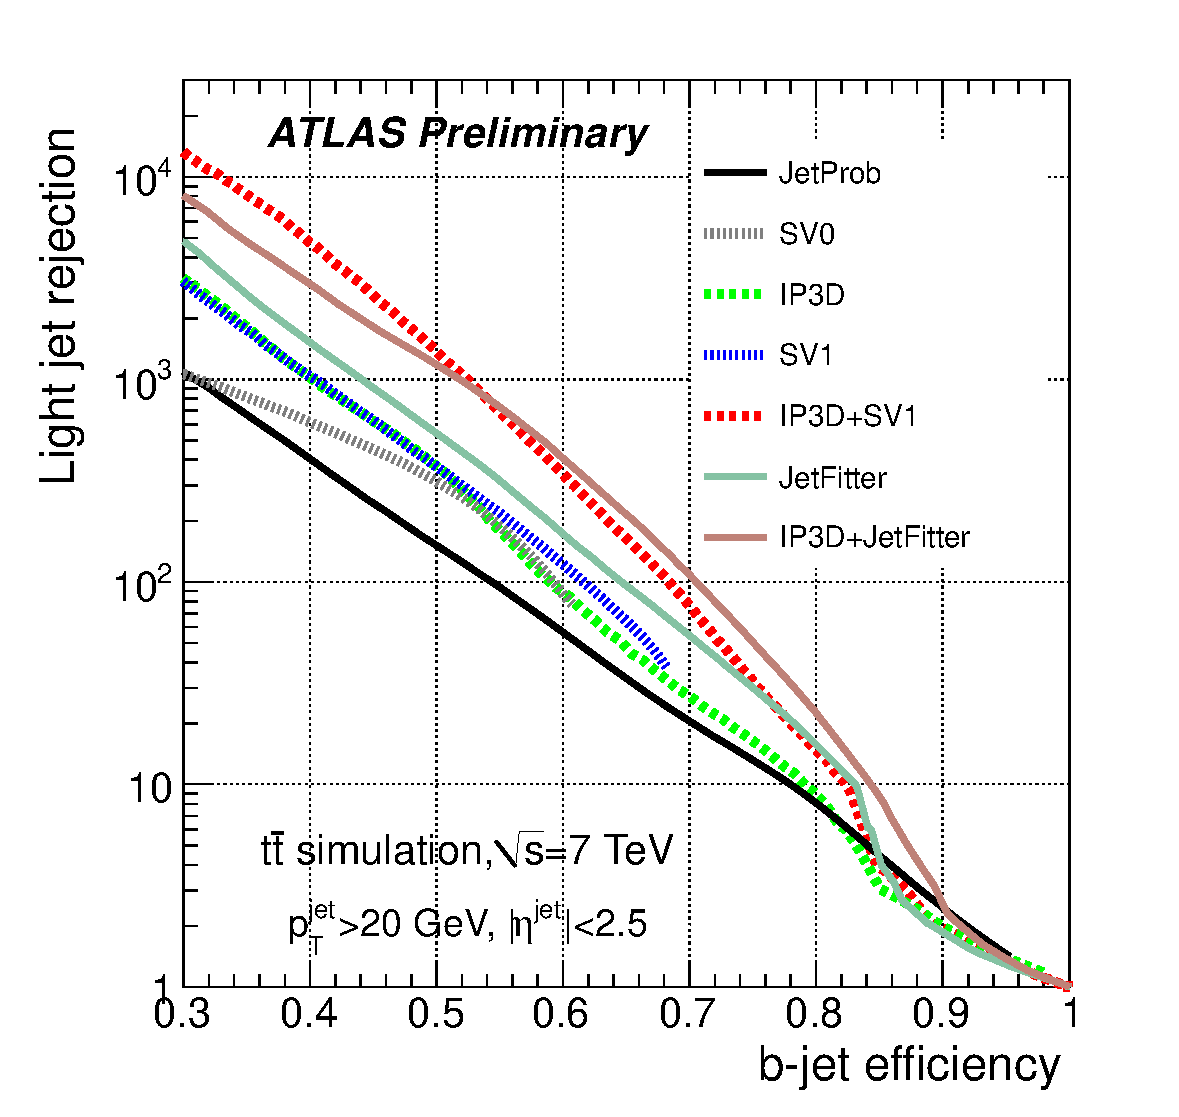
\includegraphics[width=\textwidth]{PartDetector/Plots/DetectorBtaggingPerformanceComp.eps}
  \caption[Light jet rejection as a function of the $b$-jet tagging efficiency, comparing some of taggers used at ATLAS as measured in simulated \ttbar\ events.]{Light jet rejection as a function of the $b$-jet tagging efficiency, comparing some of taggers used at ATLAS as measured in simulated \ttbar\ events~\cite{Detector:TaggingJetFitter}.}
  \label{fig:DetectorTaggingPerf}
\end{figure}

\subsubsection{The SV0 and SV1 algorithms}

The SV0 algorithm~\cite{Detector:BTaggingSV0} reconstructs secondary vertices using tracks within the cone of the candidate jet. These secondary vertices are located at a decay length $L$ from the primary vertex. A cut is then applied on the decay length significance $L/\sigma_{L}<5.72$, this is an operating point that yields a $b$-tagging efficiency of $\SI{50}{\percent}$ as measured on simulated inclusive \ttbar\ events.

The SV1 algorithm is an extension of the SV0 algorithm. In order to improve the tagging performance, three properties of the secondary vertex are used as inputs to a likelihood ratio: the invariant mass of the tracks associated to the vertex, the ratio of the sum of the energies of the tracks in the vertex to the sum of the energies of the tracks in the jet, and the number of two-track vertices. The $\DeltaR$ between the jet axis and the line joining the primary and secondary vertices is also used.

\subsubsection{The JetFitter algorithm}

The JetFitter algorithm~\cite{Detector:TaggingJetFitter} uses a Kalman filter to find a line along which the $b$, $c$ and the primary vertices lie, along with their position on the line, giving an approximated flight-path for the $b$-hadron. Discrimination is based on a likelihood using similar variables as in the SV1 algorithm and variables such as the flight length significances of the secondary vertices.

\subsubsection{The IP3D algorithm}

The IP3D algorithm makes use of the transverse and longitudinal impact parameter significances in two-dimensional histograms to discriminate between $b$, $c$ and LF jets. A likelihood-ratio method is used: the IP significances are compared to pre-defined smoothed and normalized distributions for $b$- and light-jets hypotheses. This produces a weight distribution for each model and a cut is applied to select jets. The IP3D algorithm is often combined with the JetFitter (IP3D+JetFitter) or SV1 algorithm (IP3D+SV1) to provide additional discriminating power.

\subsubsection{The MV1 algorithm}

The MV1 algorithm uses the output weights of the IP3D, SV1 and JetFitter algorithms as inputs to an artificial neural network. The working point used at ATLAS is defined so as to achieve a $b$-tagging efficiency of \SI{70}{\percent} with an associated mistag rate of less than \SI{1.5}{\percent}~\cite{DetectorBtaggingMistagMV1} depending on the pseudorapidity and transverse momentum of the jet in question. Note that this efficiency is not constant with respect to the jet \pt\ as can be seen from Figure~\ref{fig:DetectorMV1Perf}. The performance at low \pt\ degrades as the decay length is shorter so finding the secondary vertex is more difficult.

\begin{figure}[htbp]
  \centering
  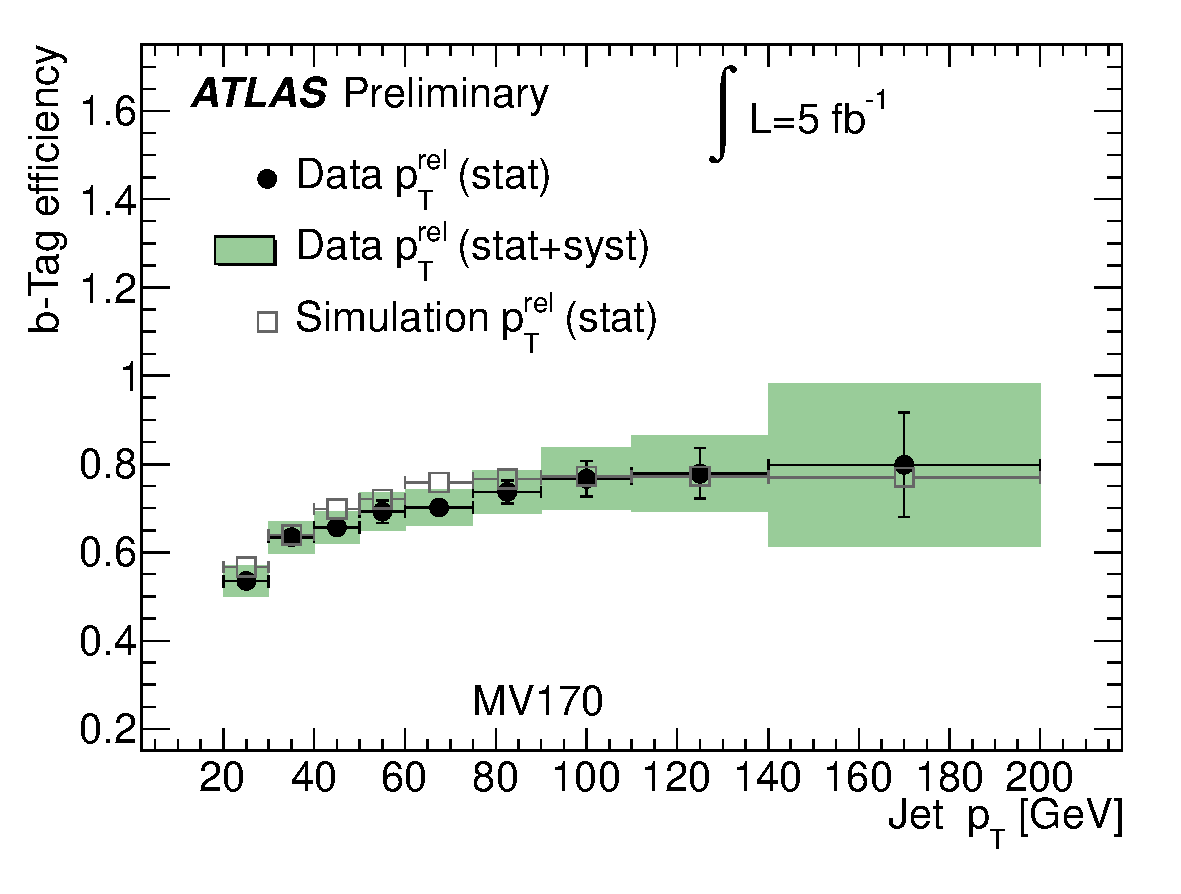
\includegraphics[width=0.75\textwidth]{PartDetector/Plots/MV1TaggerEff.pdf}
  \caption[The b-tag efficiency in data and simulation for the MV1 algorithm at the \SI{70}{\percent} efficiency point, with respect to jet transverse momentum.]{The b-tag efficiency in data and simulation for the MV1 algorithm at the \SI{70}{\percent} efficiency point, with respect to jet transverse momentum~\cite{Detector:MV1TaggerEffs}.}
  \label{fig:DetectorMV1Perf}
\end{figure}

\subsubsection{Soft lepton tagging} \label{sec:DetectorSLT}

\emph{Soft lepton tagging} (SLT) algorithms attempt to identify leptons produced in the semileptonic decay of $b$ and $c$ quarks for the purpose of determining the presence of HF quarks. The term ``semileptonic'' here refers to the decay of a $b$-hadron in such a way as to produce a lepton-neutrino pair with an additional hadron. The lepton produced is known as a \emph{soft} lepton due to its relatively low transverse momentum.

A soft muon can be produced in a variety of ways starting from a $b$-quark, either directly via $b\rightarrow \mu\bar{\nu}_{\mu}X$, where $X$ is any hadron; or indirectly, via a $c$, $\bar{c}$ or a $\tau$ lepton. The direct and indirect via a $c$ production mechanisms are shown in Figure~\ref{fig:DetectorSLTFeynm}. The branching ratio for each of these decays is shown in Table~\ref{tab:DetectorSLTBR}. The total BR for the production of a soft muon from a $b$ quark is \SI[multi-part-units=single]{20.1(10)}{\percent}, thus the probability for a \ttbar\ event to contain at least one semileptonic $b$ decay is approximately \SI{36}{\percent}.

\begin{figure}[htbp]
  \centering
    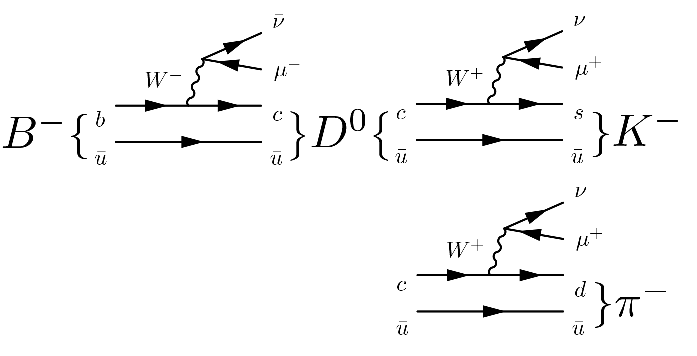
\includegraphics[width=0.75\textwidth]{PartDetector/Diagrams/SemiLeptonicDecay.pdf}
    \caption[Feynman diagram of one of the mechanisms for lepton production via semileptonic $b$ decay.]{Feynman diagram of one of the mechanisms for lepton production via semileptonic $b$ decay. Shown are the direct $b\rightarrow \mu$ and indirect $b\rightarrow c\rightarrow\mu$.}
  \label{fig:DetectorSLTFeynm}
\end{figure}

\begin{table}[htbp]
  \centering
    \begin{tabular}{@{}lS[table-format=2.2(2)]@{}}
      \toprule
      Mode                                        & {Muon BR [\si{\percent}]} \\
      \midrule % -------------------------
      $b\rightarrow \mu^{-}$                      & {$\num{10.95}\;^{+\;0.29}_{-\;0.25}$} \\
      $b\rightarrow c \rightarrow \mu^{+}$        & 8.02(19) \\
      $b\rightarrow \bar{c} \rightarrow \mu^{-}$  & 1.6(5) \\
      $b\rightarrow \tau^{-} \rightarrow \mu^{-}$ & 0.42(4) \\
      \midrule % -------------------------
      All modes                                   & 21.0(10) \\
      \bottomrule % -------------------------
    \end{tabular}
    \caption[Branching ratio for the production of a muon from a $b$-quark in both direct and indirect modes.]{Branching ratio for the production of a muon from a $b$-quark in both direct and indirect modes~\cite{Theory:PDGBooklet}.}
  \label{tab:DetectorSLTBR}
\end{table}

The soft muon tagger used in this analysis is based on the quality of the fit between the ID track and MS track as represented by the \xsm. Several tagger-specific cuts (summarized in Table~\ref{tab:DetectorSMTCuts}) are placed on the candidate muons and jets. Candidate SMT muons are required to lie within the coverage of the ID and have sufficient transverse momentum for reliable reconstruction. Requirements are made on the impact parameters of the muon ID track to remove contributions from spurious matches between ID and MS tracks, and from pile-up vertices. Finally, the main cut on the quality of the fit $\xsd=\xsm/\ndof$ is set at less than \num{3.2}. This is an operating-point that provides a $b$-jet (semileptonic $b$-jet) identification efficiency of \SI{10}{\percent} (\SI{50}{\percent}) and a LF rejection factor of 200 per jet. Candidate jets are required to have more than three charged tracks associated with them or a jet EM fraction smaller than \num{0.8}. These criteria ensure that the jet did not originate from the muon itself. Finally, the muon is associated to the jet with a cut $\DeltaR_{\mu}^{\textrm{jet}}<0.5$. The following chapter describes the calibration of the SMT tagger.

\begin{table}[htbp]
\ra{1.2}
  \centering
  \begin{tabular}{ll}
  \toprule
  \multicolumn{2}{c}{\textbf{Muon cuts}} \\
  \midrule
  Muon to jet association & $\DeltaR_{\mu}^{\textrm{jet}}<0.5$ \\
  \multirow{2}{*}{Reconstruction} & $|\eta|<2.5$ \\
                                  & $\pt>\SI{4}{GeV}$ \\
  \multirow{2}{*}{Pile-up reduction} & $|d_0|<\SI{3}{\mm}$ \\
                         & $|z_0\sin{\theta}|<\SI{3}{\mm}$ \\
  Track matching quality & $\xsd<3.2$ \\
  \midrule
  \multirow{2}{*}{Muon-jet rejection} & Jet $N^{\textrm{charged}}_{\textrm{trk}} > 3$ \textbf{or} \\
    & $\textrm{Jet EM fraction} < \num{0.8}$ \\
  \bottomrule
  \end{tabular}
  \caption{Jet and muon SMT Cuts.}
  \label{tab:DetectorSMTCuts}
\end{table}

% !TEX root = ../Thesis.tex
\newcommand{\JMu}{\ensuremath{\jpsi\rightarrow\mu\mu}}
\newcommand{\ZMu}{\ensuremath{Z\rightarrow\mu\mu}}
\newcommand{\errt}[2]{\ensuremath{\pm\num{#1}\,\textrm{#2}}}
\newcommand{\fulleff}[4]{\ensuremath{(\num{#1}\errt{#2}{(bkg.)}\,\errt{#3}{(sig.)}\,\errt{#4}{(stat.)})\si{\percent}}}
\newcommand{\Nyield}[2]{\ensuremath{ N^{ \textrm{#1} }_{\textrm{#2}} } }

\chapter[Calibration of the soft muon tagger]{Calibration of the soft muon tagger for 2012 ATLAS data}\label{ch:Calibration}

High-energy physics relies heavily on the use of simulated data to inform the development of analysis techniques. It paramount that the simulation reflect nature as closely as possible. However, the simulation cannot perfectly recreate conditions within the detector and some kinematic variables are not accurately simulated. This includes the quality of matching between ID and MS tracks which if fundamental for the SMT tagger.

Selection and reconstruction techniques are said to be calibrated when the discrepancy between simulation and collision data is quantified. This process has to be repeated on new collision data and/or when simulation is changed in a relevant and significant way.

In the case of muon reconstruction method and the \xsm\ tagger it is important that the difference in efficiency between simulation and collision data be accounted for. This is done by defining a scale factor (SF),

\begin{equation}
  \textrm{SF} = \frac{\epsilon^{\textrm{Data}}}{\epsilon^{\textrm{MC}}}
\end{equation}
%
which is used to rescale the simulation so that it better represents the data.

One of the advantages of using the \xsm\ tagger over other forms of $b$-tagging is that the presence of a jet is not required to measure the \xsm\ of a muon. This means that the calibration can be performed on isolated muons such as those from \JMu\ or \ZMu\ using the so called tag and probe method. This calibration relies on muons with low \pt\ from \jpsi\ decays.

The tag and probe method is implemented as follows: a STACO combined muon is designated as the \emph{tag}, this muon must pass a stringent set of cuts implying that this is indeed a muon from a \jpsi. the second muon which is designated as the \emph{probe} is simply an ID track. To ensure that the probe is the second muon from the \jpsi\ decay, the invariant mass of the combined tag and probe system is required to be in a window centred around the \jpsi\ mass. The complete selection used in the calibration is detailed in Section~\ref{sec:CalibrationSelection}. These probes are used to measure the reconstruction efficiency and the \xsm\ tagger efficiency as using a fit to the invariant mass distribution as describe in Section~\ref{sec:CalibrationFitting}. The results of this analysis are then presented in Section~\ref{sec:CalibrationEfficiencies}.

The analysis used here is based on a previous calibration of the \xsm\ tagger performed on 2011 ATLAS collision data detailed in~\cite{Calibration:MattThesis}. The analysis presented here differs from the 2011 calibration in several ways which will be highlighted and explained.

\subsection*{Software, collision data and simulated samples}

The dataset used is made of those luminosity blocks selected by the recommended standard \emph{good runs list} (GRL) which corresponds to all $pp$ collision periods in 2012. The GRL selects only those luminosity blocks where detector conditions are appropriate for physics data-taking. This requires that all relevant detector components are operational, and that stable beam conditions have been achieved. The datasets are part of the 2013 summer reprocessing corresponding to data taken in periods A through to L, excluding periods F and J. In total this represents an integrated luminosity of \SI{20.1}{\per\femto\barn}. 

The efficiency scale factor is measured against a sample containing almost 10 million \JMu\ events. At event generation, filters are applied so the sample only contains events where both truth muons have a momentum of at least \SI{4}{\GeV} and they must lie within the pseudorapidity range $|\eta|<2.5$. This selection matches the object selection used by most analyses. 

\section{Tag and probe selection}\label{sec:CalibrationSelection}

The tag and probe procedure is as follows: first, require the presence of a STACO CB muon which passes a very stringent selection. This strongly implies that this is a real muon and thus is labelled as the tag. A very loose selection is then applied to all ID tracks to construct a pool of candidate probes. Pairs of tag and probes are formed by requiring that the combined invariant mass lie within a \jpsi\ mass window and the pair pass additional pairing cuts. This then implies that the probe is likely the other muon from the \jpsi\ decay and as such is a suitable test-bed to measure the performance of the muon reconstruction algorithm. All selection criteria are detailed and explained in Section~\ref{sec:CalibrationSelectionCuts}.

Probes which are reconstructed into STACO CB muons are labelled as muon probes. The reconstruction performance is quantified by the portion of probes, which are likely from real muons, that are reconstructed into muons. The performance of the \xsm\ tagger is estimated in a similar way, by measuring the proportion of muon probes which are selected by the \xsm\ algorithm.

\subsection{Trigger requirements}\label{sec:CalibrationTriggerRequirement}

In order for an event to be included in the analysis it must pass at least one of the trigger chains listed in Appendix~\ref{app:CalibrationTrigger}. For the sake of brevity only the primary trigger, EF\_mu6\_Trk\_Jpsi\_loose which contributes the majority of events, is described here.

As stated in the trigger name, this is an EF trigger which requires the presence of a muon with a momentum of at least \SI{6}{GeV} and an ID track with a combined invariant mass in the range $\SI{2.6}{GeV}<m_{\textrm{inv}}<\SI{3.6}{GeV}$. This mass window is loose enough to   contain the entirety of the \jpsi\ peak and side-bands that allow for background removal. Double muon triggers are not used to avoid introducing a bias by requiring the presence of two good muons. 

While all triggers are operational in all periods, most are heavily prescaled by a factor which is period dependent. This does not have a first-order effect on the efficiency as only ratios of event yields are compared between collision data and simulation. However, the effective integrated luminosity is reduced to approximately \SI{200}{\per\nano\barn} as a result of the prescale. A short study was carried out to examine the effects of multiple prescaled triggers on the scale factors. The measurement was carried out using only the primary trigger and the results were compared to the nominal calibration which included all the triggers, no significant discrepancy between the two was observed.

\subsection{Selection cuts}\label{sec:CalibrationSelectionCuts}

The selection criteria for tags, probes, muon probes and SMT muons are listed and detailed below. All cuts are applied on the kinematic properties as measured in the ID due to its improved resolution. Also note that all objects must pass a set of track quality criteria as recommended by the ATLAS \emph{muon combined performance} (MCP) group. These cuts require a certain number of detector elements be active to ensure good quality track reconstruction. The selection criteria are listed in Appendix~\ref{app:CalibrationMCPCuts}.

The tag selection is summarized in Table~\ref{tab:CalibrationTagSelection}. The tag is a STACO combined muon with a pseudorapdity and transverse momentum that allow for reliable reconstruction. The requirements on the impact parameter variables are in place to remove spurious muons from pile-up events and the decay-in-flight of long-lived hadrons. Finally, the tag muon is required to have fired at least one of the triggers under which the event was recorded. This is done by matching the reconstructed trigger object to the tag muon via a $\Delta R$ cut of less than \num{0.01}.

\begin{table}
  \centering
    \begin{tabular}{@{}ll@{}}
    \toprule
    \multicolumn{2}{c}{Tag selection} \\
    \midrule
    \multirow{3}{*}{Reconstruction cuts} & STACO combined muon \\
                                      & $|\eta|<2.5$ \\
                                      & $\pt>\SI{4}{\GeV}$ \\
    \multirow{4}{*}{Pileup reduction} & $|d_{0}|<\SI{0.3}{\mm}$ \\ 
                                      & $|z_{0}|<\SI{1.5}{\mm}$ \\
                                      & $|d_{0}/\sigma_{d_{0}}|<3$ \\
                                      & $|z_{0}/\sigma_{z_{0}}|<3$ \\
    \bottomrule  
    \end{tabular}
    \caption{Tag selection criteria.}\label{tab:CalibrationTagSelection}
\end{table}

The probe selection is a subset of the tag selection and only requires an ID track with $|\eta|<2.5$ and $\pt>\SI{4}{\GeV}$. 

The pairing selection, summarized in Table~\ref{tab:CalibrationPairingSelection}, is designed to construct pairs tag candidates and probe candidate which likely come from the same \jpsi\ decay. The main component of the selection is the invariant mass window cut. The tag and the probe are required to be well separated in $\eta$-$\phi$ space to prevent the objects from entering each others isolation cones.

\begin{table}[htbp]
  \centering
    \begin{tabular}{@{}ll@{}}
      \toprule
      \multicolumn{2}{c}{Pairing criteria} \\
      \midrule
      Opposite charge   & $q_{\textrm{tag}} \neq q_{\textrm{probe}}$ \\
      Mass window       & $|m_{\jpsi}-m_{\textrm{tag, probe}}|\leq\SI{2}{\GeV}$ \\
      Overlap reduction & $0.2<\Delta R^{\textrm{tag}}_{\textrm{probe}}<3.5$ \\
      Pileup reduction  & $\Delta z_{0}<\SI{0.2}{\mm}$ \\
      \bottomrule
    \end{tabular}
    \caption{Pairing criteria.}\label{tab:CalibrationPairingSelection}
\end{table}

In the 2011 calibration analysis, the track of the tag and the probe were refitted to a common vertex and the quality of the refit, expressed by a $\chi^2$, was part of the pairing criteria. This cut is meant to reduce the effects of pile-up on the measurement by ensuring both objects have a common origin. It is not possible to perform such a refit here, since the data format used for this analysis is a derived form of that used in 2011. Instead, a cut on $\Delta z_{0}=|z_{0,\textrm{ tag}}-z_{0,\textrm{ probe}}|$ is applied. If several pairings are made for a single tag, the pair with the smallest $\Delta z_{0}$ is used.

The STACO CB reconstruction efficiency is not measured by applying the algorithm on the probe collection but rather a probe is said to be a muon probe if it matches a combined muon from the STACO collection. This is done by requiring the \DeltaR\ between the probe and the STACO CB muon be less than \num{0.01}. Probes which are matched become the numerator of the reconstruction efficiency and the denominator is defined as the number of probes:

\begin{equation}
  \epsilon_{\textrm{reco}} = \frac{N_{\textrm{muon probe}}}{N_{\textrm{probe}}}
\end{equation}

A muon probe is said to be an SMT muon if it passes the selection listed in Table~\ref{tab:CalibrationSMTSelection} which matches the cuts defined in Section~\ref{sec:DetectorSLT}. The \xsd\ distribution of muon probes is shown in Figure~\ref{fig:CalibrationMatchChi2Dist}.

\begin{table}[htbp]
  \centering
    \begin{tabular}{@{}ll@{}}
      \toprule
      \multicolumn{2}{c}{SMT selection} \\
      \midrule
      \multirow{2}{*}{Pileup reduction} & $|d_{0}|<\SI{3}{\mm}$ \\
                            & $|z_{0}\sin(\theta)|<\SI{3}{\mm}$ \\
      Match quality         & $\xsm/\ndof<3.2$ \\
      \bottomrule
    \end{tabular}
    \caption{SMT criteria.}\label{tab:CalibrationSMTSelection}
\end{table}

\begin{figure}[htbp]
  \centering
    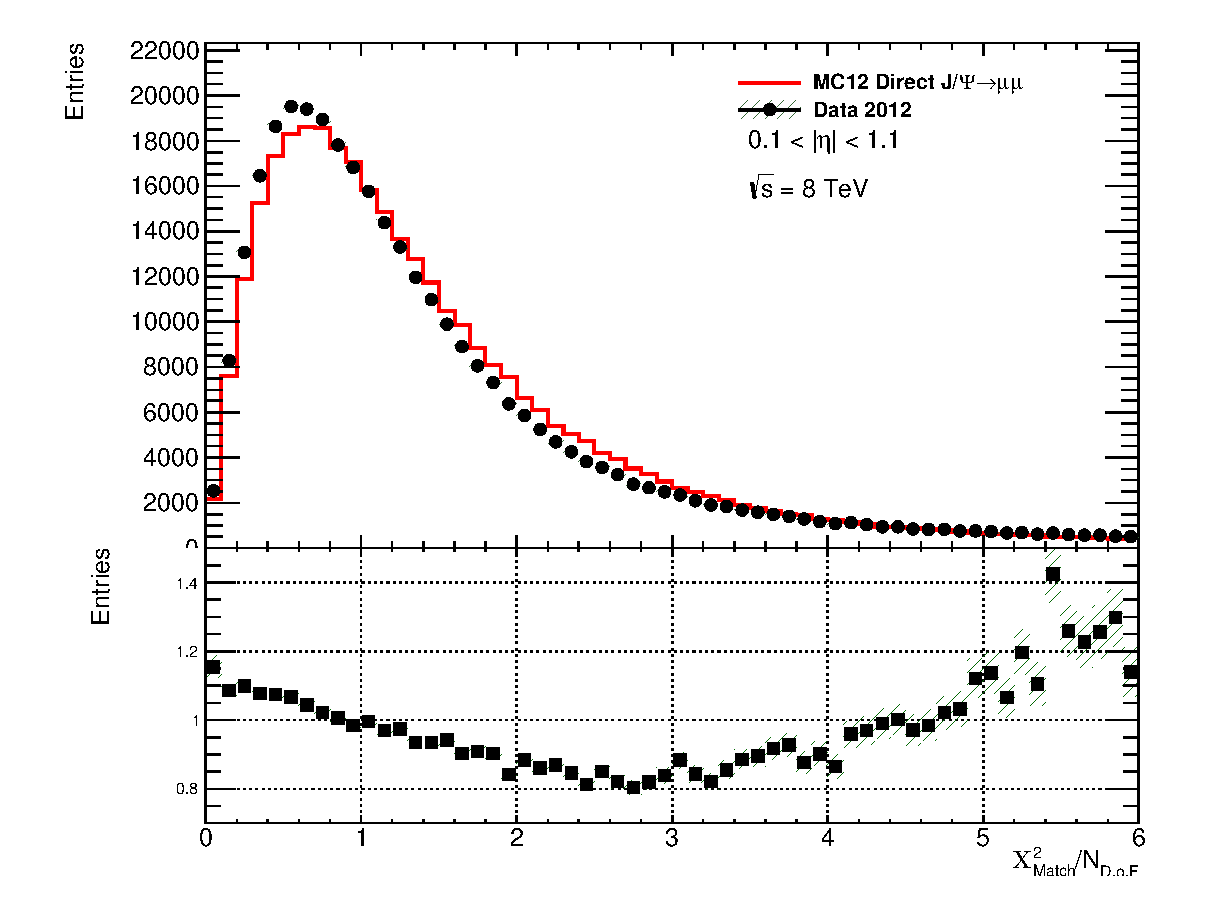
\includegraphics[width=0.75\textwidth]{PartCalibration2012/Plots/Kinematics/h_muonprobe_matchchi2_ndof_Nominal.eps}
    \caption[The distribution of \xsd\ for all muon probes for ATLAS collision data and prompt simulated \jpsi.]{The distribution of \xsd\ for all muon probes for ATLAS collision data (solid dots) and simulated prompt \jpsi\ (solid line). Note that the collision data distribution includes sources of background.}\label{fig:CalibrationMatchChi2Dist}
\end{figure}

The denominator of the SMT efficiency is the number of muon probes and the numerator is the number of muon probes which pass the SMT selection:

\begin{equation}
  \epsilon_{\textrm{SMT}} = \frac{N_{\textrm{SMT}}}{N_{\textrm{muon probe}}}
\end{equation}

\section{Invariant mass fitting}\label{sec:CalibrationFitting}

The pairing criteria are very effective at selecting \jpsi\ events, however non-\jpsi\ background events also pass the selection. These include combinatorial background where the wrong tag and probe pair is constructed, and Drell-Yan which appears as a continuum below the \jpsi\ peak.

The number of probes is extracted from a fit to the invariant mass of the dimuon system. The invariant mass is fitted with the sum of a quadratic polynomial, for the background; and a Gaussian function, for the signal. The yield is obtained by subtracting the integral of the background function from the binned data, this is used instead of relying on an accurate fit to the signal peak.

The integration is performed in a window with a width three larger than the width of the fitted Gaussian, denoted as $3\sigma$ in Figure~\ref{fig:CalibrationFittingExample}. The composite fit line, the background-only distribution and the implied signal Gaussian peak are also shown.

\begin{figure}[htbp]
  \centering
    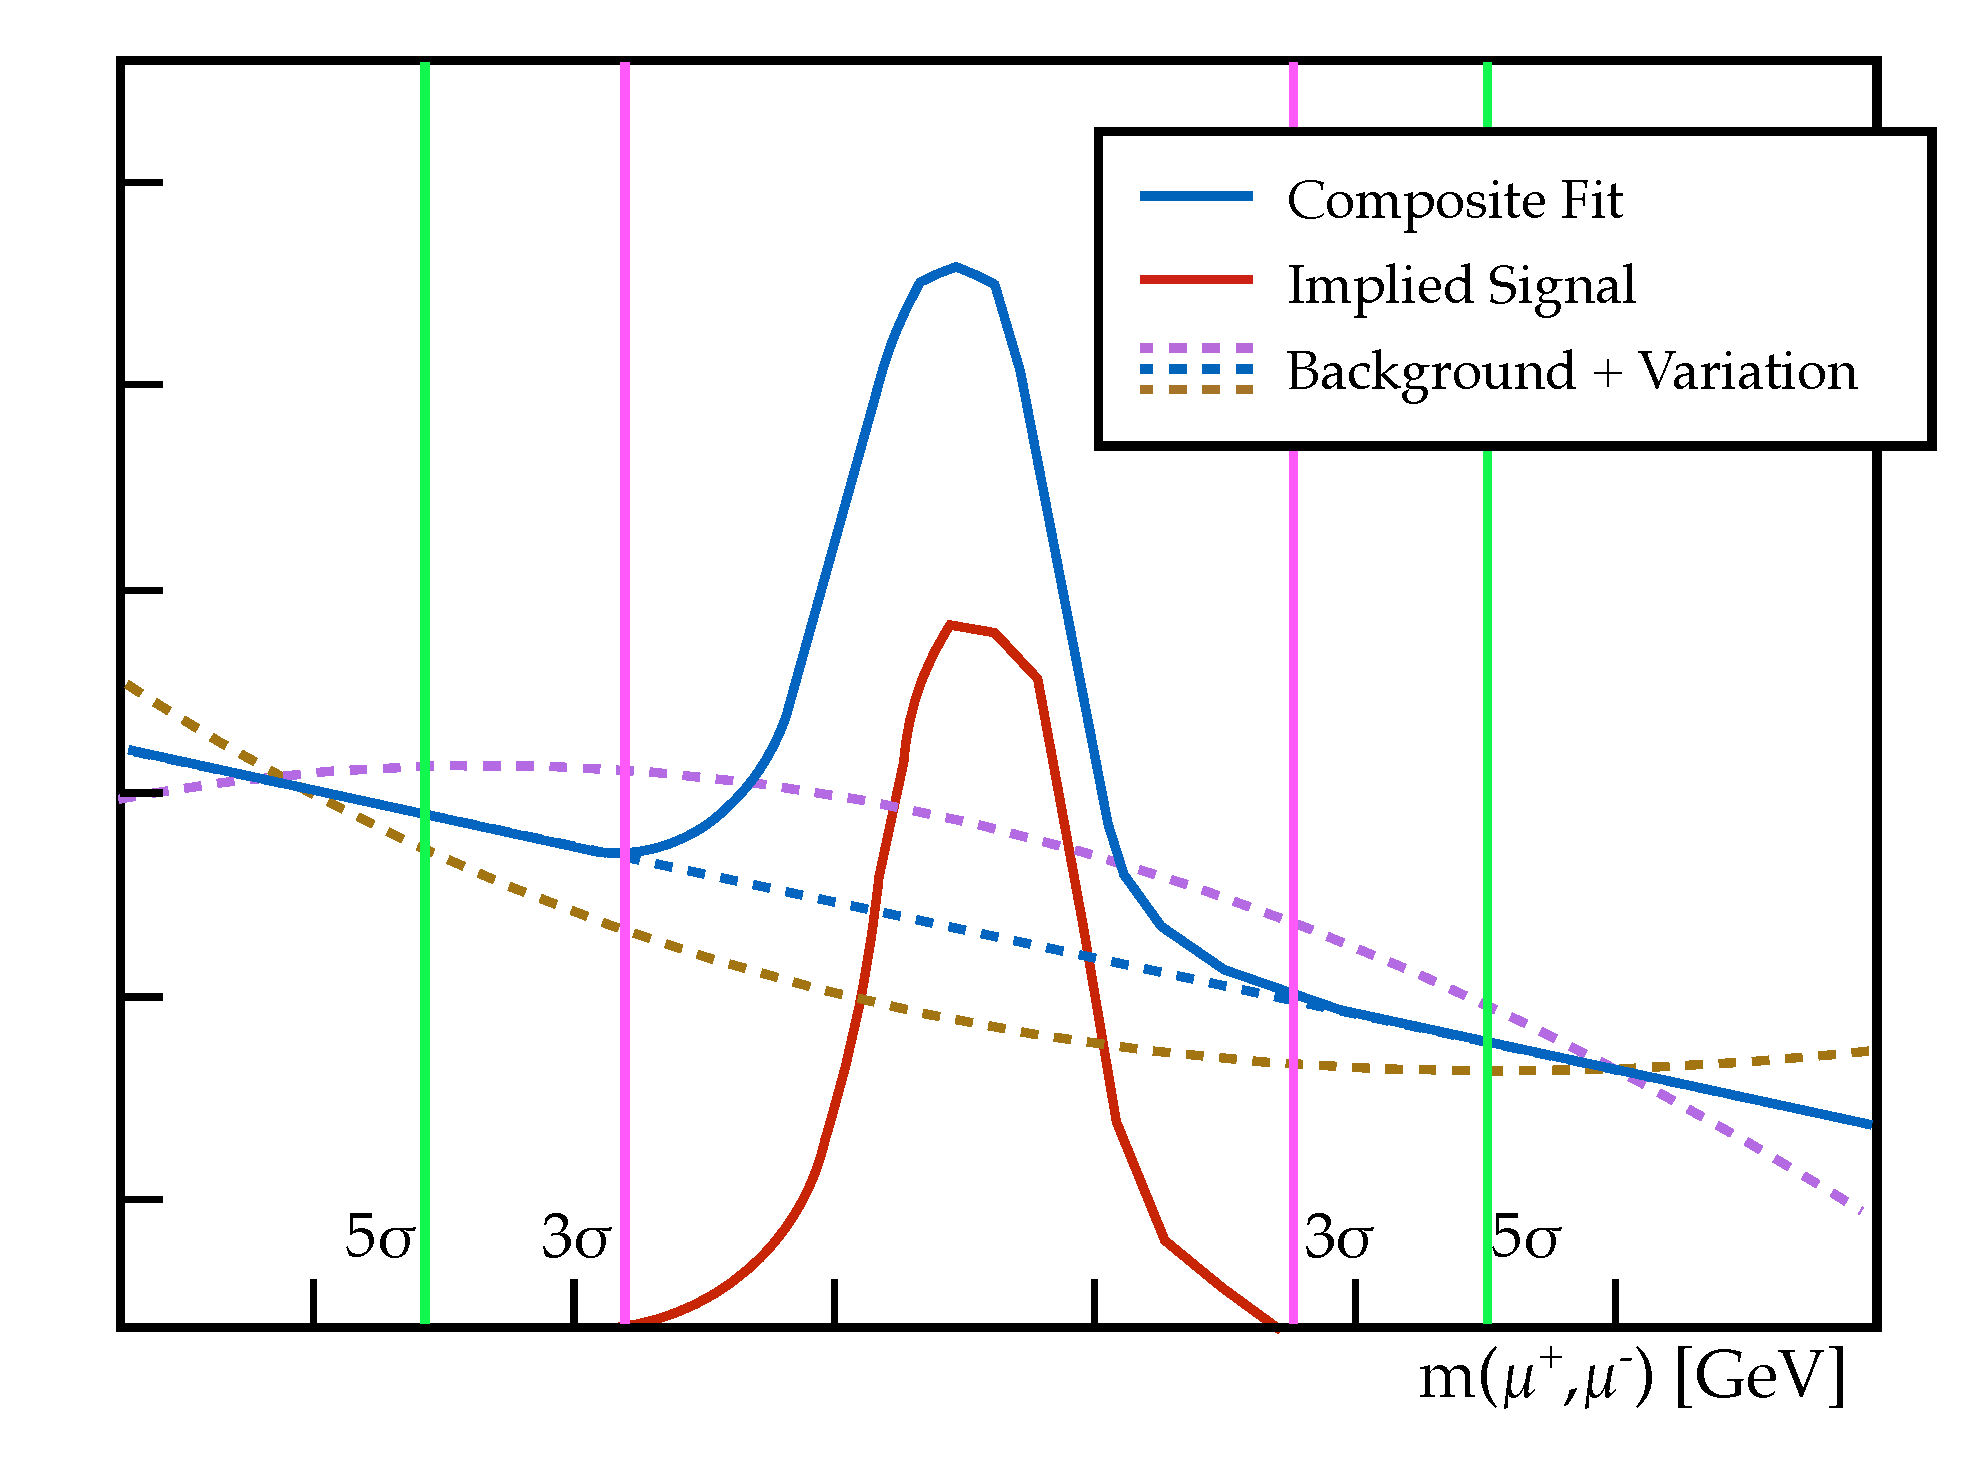
\includegraphics[width=0.75\textwidth]{PartCalibration2012/Plots/FittingExample.pdf}
    \caption[Drawing of the components of the fitting procedure.]{Drawing of the components of the fitting procedure. The composite fit is shown along with the corresponding implied signal and background. The two variations of the background shape are also shown, these are exaggerated for illustration purposes.}\label{fig:CalibrationFittingExample}
\end{figure}

The \jpsi\ peak does not follow a Gaussian shape exactly, but rather the best fit is obtained by the so-called Crystal Ball function shown in Figure~\ref{fig:CalibrationCBDist}. This is a convolution of a Gaussian function with a power tail at low invariant mass to account for the energy loss due to photon emission.

\begin{figure}[htbp]
  \centering
  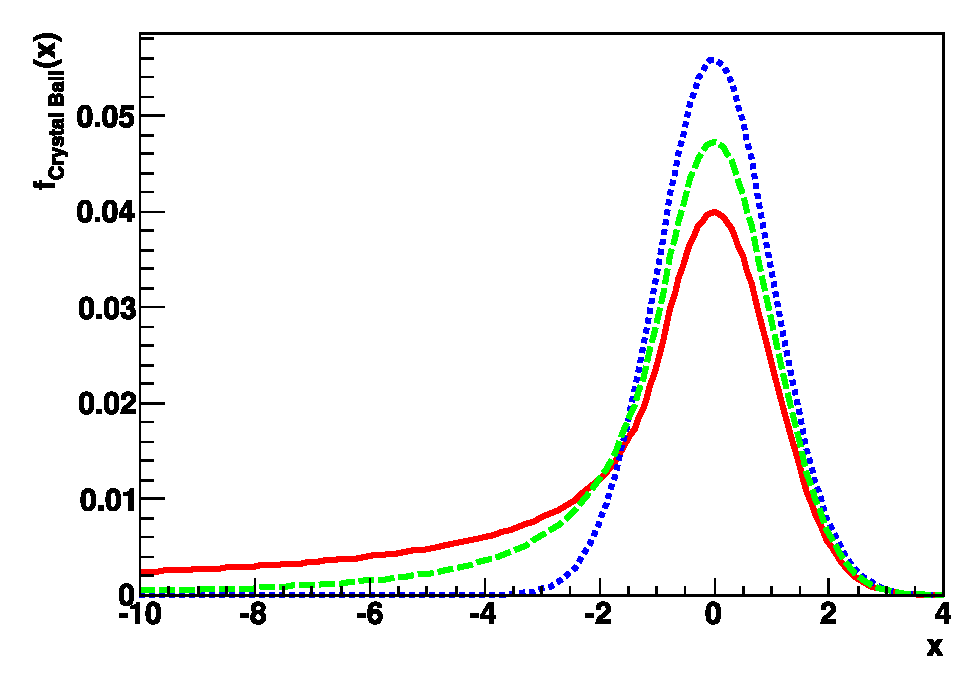
\includegraphics[width=0.75\textwidth]{PartCalibration2012/Plots/CrystalBallFunction.eps}
  \caption[Diagram of crystal ball distributions with varying tail sizes.]{Diagram of crystal ball distributions with varying tail sizes. Obtained from Ref.~\cite{Calibration:CBFunction} and modified.}\label{fig:CalibrationCBDist}
\end{figure}

Different combinations of signal and background functions were tested to determine the most stable combination. For the signal, the sum of two Gaussian functions was tested, while for the background a linear function, an exponential function, and the sum of two exponential functions were tried. It was found that none of these yielded good stable fits in the entire pseudorapidity range. For example, the linear function resulted in a mismodelling of the background at the probe level which led to negative efficiencies or extremely large uncertainties. 

From an operational perspective, using a Gaussian function allowed for good stable fits over the hundreds of bins used, and simplified the fitting procedure as a whole. Any mismodelling of the background because of the choice of a Gaussian in lieu of the Crystal Ball fit, is taken into account by the background uncertainty described in the next section.

Several different sets of initial fit conditions were tested and those which yielded the best and most stable fits across the entire $\eta$ and \pt\ range were used. 

The width at the probe level is obtained from the fit and is then used in the fits to the muon probe and SMT distributions. The mean is obtained independently from the fit to each individual distributions. The mean is expected to lie very close to the true \jpsi\ mass, however this is not forced in the fitting procedure. Instead the fit is allowed to set the mean in a window with a width of approximately \SI{1.2}{\GeV}. 

\subsection{Uncertainty measurement}\label{sec:CalibrationUncertainty}

The uncertainty on the efficiency is made up of three components: the statistical uncertainty on the efficiency is estimated as a binomial error,
%
\begin{equation}
  \sigma_{\textrm{stat.}} = \sqrt{\frac{\epsilon(1-\epsilon)}{N}}
\end{equation}
%
where $\epsilon$ is the measured efficiency and $N$ is, in this case the denominator of the efficiency measured.

The second component of the efficiency uncertainty quantifies the error in the background fit. The uncertainty is determined by constructing two functions that denote the maximum upward and downward fluctuation of the background fit. The efficiency is measured using one of these fluctuations and the result is compared to the nominal efficiency.

After the fit of the composite function is carried out, a downward variation of the background is defined as:
%
\begin{equation}
  f^{\textrm{down}}(x) = a_{\textrm{min}}x^{2} + b_{\textrm{max}}x + c_{\textrm{min}}\textrm{, where }p_{\textrm{max/min}}=p_{\textrm{central}}\pm\sigma_{p}
\end{equation}
%
where the maximum and minimum of a parameter is obtained by varying its central value by the uncertainty obtained from the fit. The upward variation of the background fit is defined as the opposite:
%
\begin{equation}
  f^{\textrm{up}}(x) = a_{\textrm{max}}x^{2} + b_{\textrm{min}}x + c_{\textrm{max}}
\end{equation}

These background variations result in the maximum deviation from the nominal integral (Figure~\ref{fig:CalibrationFittingExample}). The uncertainty on the efficiency is determined by obtaining the maximum efficiency in both directions. If the nominal efficiency is defined as
%
\begin{equation}
  \epsilon_{\textrm{nominal}} = \frac{\Nyield{nominal}{numerator}}{\Nyield{nominal}{denominator}}
\end{equation}
%
then the variations are defined as,
%
\begin{equation}
  \epsilon_{\textrm{up}} = \frac{\Nyield{up}{numerator}}{\Nyield{down}{denominator}}%
  \textrm{,}\qquad%
  \epsilon_{\textrm{down}} = \frac{\Nyield{down}{numerator}}{\Nyield{up}{denominator}}
\end{equation}
%
where \Nyield{up/down}{}\ are the yields obtained from the integration of the upward/downward variations of the background function.

Finally the uncertainty on the background is given by the average of the differences between $\epsilon_{\textrm{up}}$ and $\epsilon_{\textrm{down}}$, and the nominal efficiency:
%
\begin{equation}
  \sigma_{\textrm{bkg}} = \frac{1}{2}(|\epsilon_{\textrm{up}}-\epsilon_{\textrm{nominal}}| + |\epsilon_{\textrm{down}}-\epsilon_{\textrm{nominal}}|)
\end{equation}

The final component of the uncertainty is obtained by varying the integration window. The nominal value is defined as $3\sigma_{\textrm{gaus}}$ away from the centre of the fitted Gaussian. An uncertainty is constructed by measuring the efficiency with a wide integration window corresponding to $5\sigma$. The integration window uncertainty is defined as:
%
\begin{equation}
  \sigma_{\textrm{sig.}} = |\epsilon_{5\sigma}-\epsilon_{3\sigma}|
\end{equation}

The total uncertainty on the efficiency is given by the sum in quadrature of all the uncertainty components. The uncertainty on the efficiency is then carried over to the scale factor determination.
As expected the invariant mass distribution for all probes contains a large amount of background, particularly in data (Figure~\ref{fig:CalibrationFittingResult}). The ``shoulders'' at each side of the \jpsi\ peak are the result of the main \jpsi\ trigger which includes a mass window cut more stringent than that required by the pairing selection. Requiring that the probe match a STACO CB muon greatly reduces the amount of background. Applying the SMT requirements also reduces the background though not as substantially.

\begin{figure}[thbp]
  \centering
    \begin{subfigure}[b]{0.54\textwidth}
    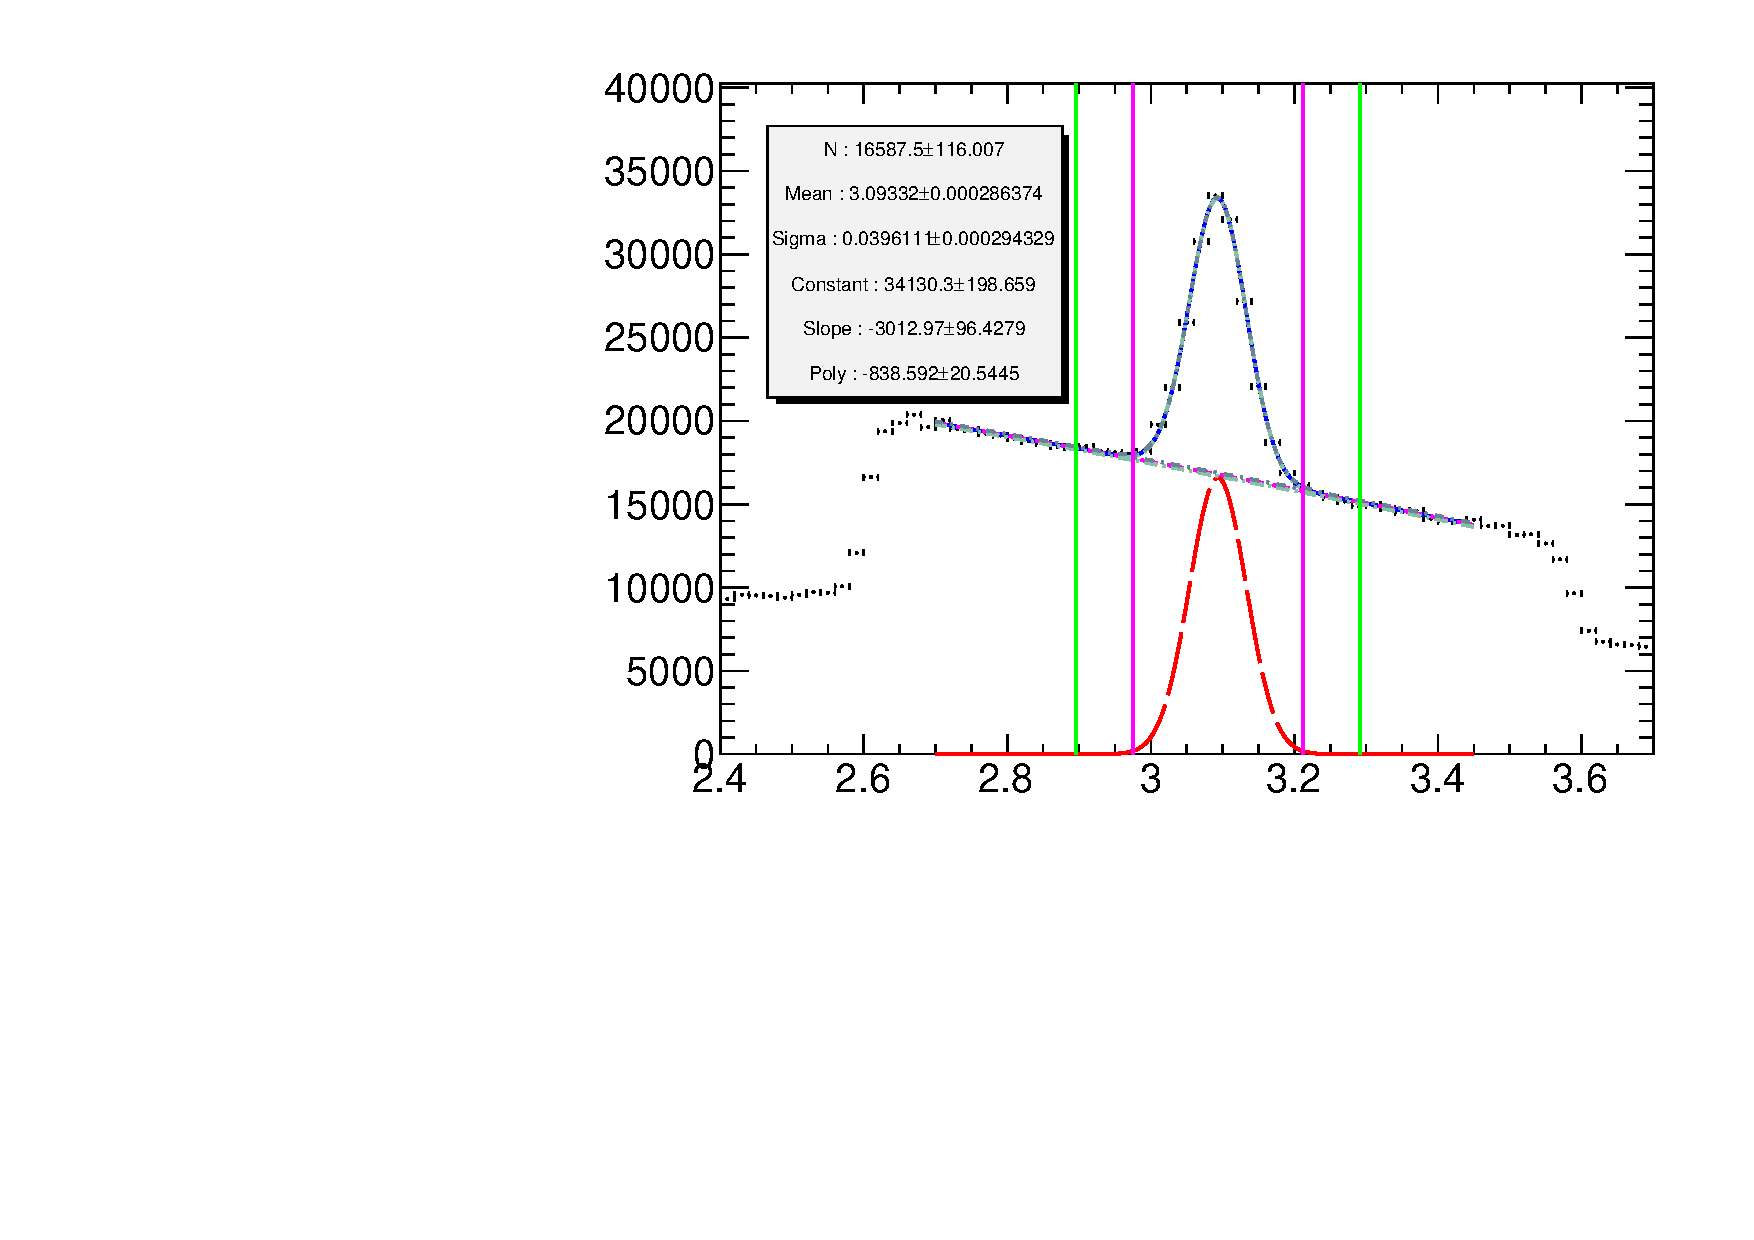
\includegraphics[width=\textwidth]{PartCalibration2012/Plots/Kinematics/Data_InvMass_pt_5_6_barrel_probe.pdf}
      \caption{Probe level}
    \end{subfigure}

    \begin{subfigure}[b]{0.54\textwidth}
      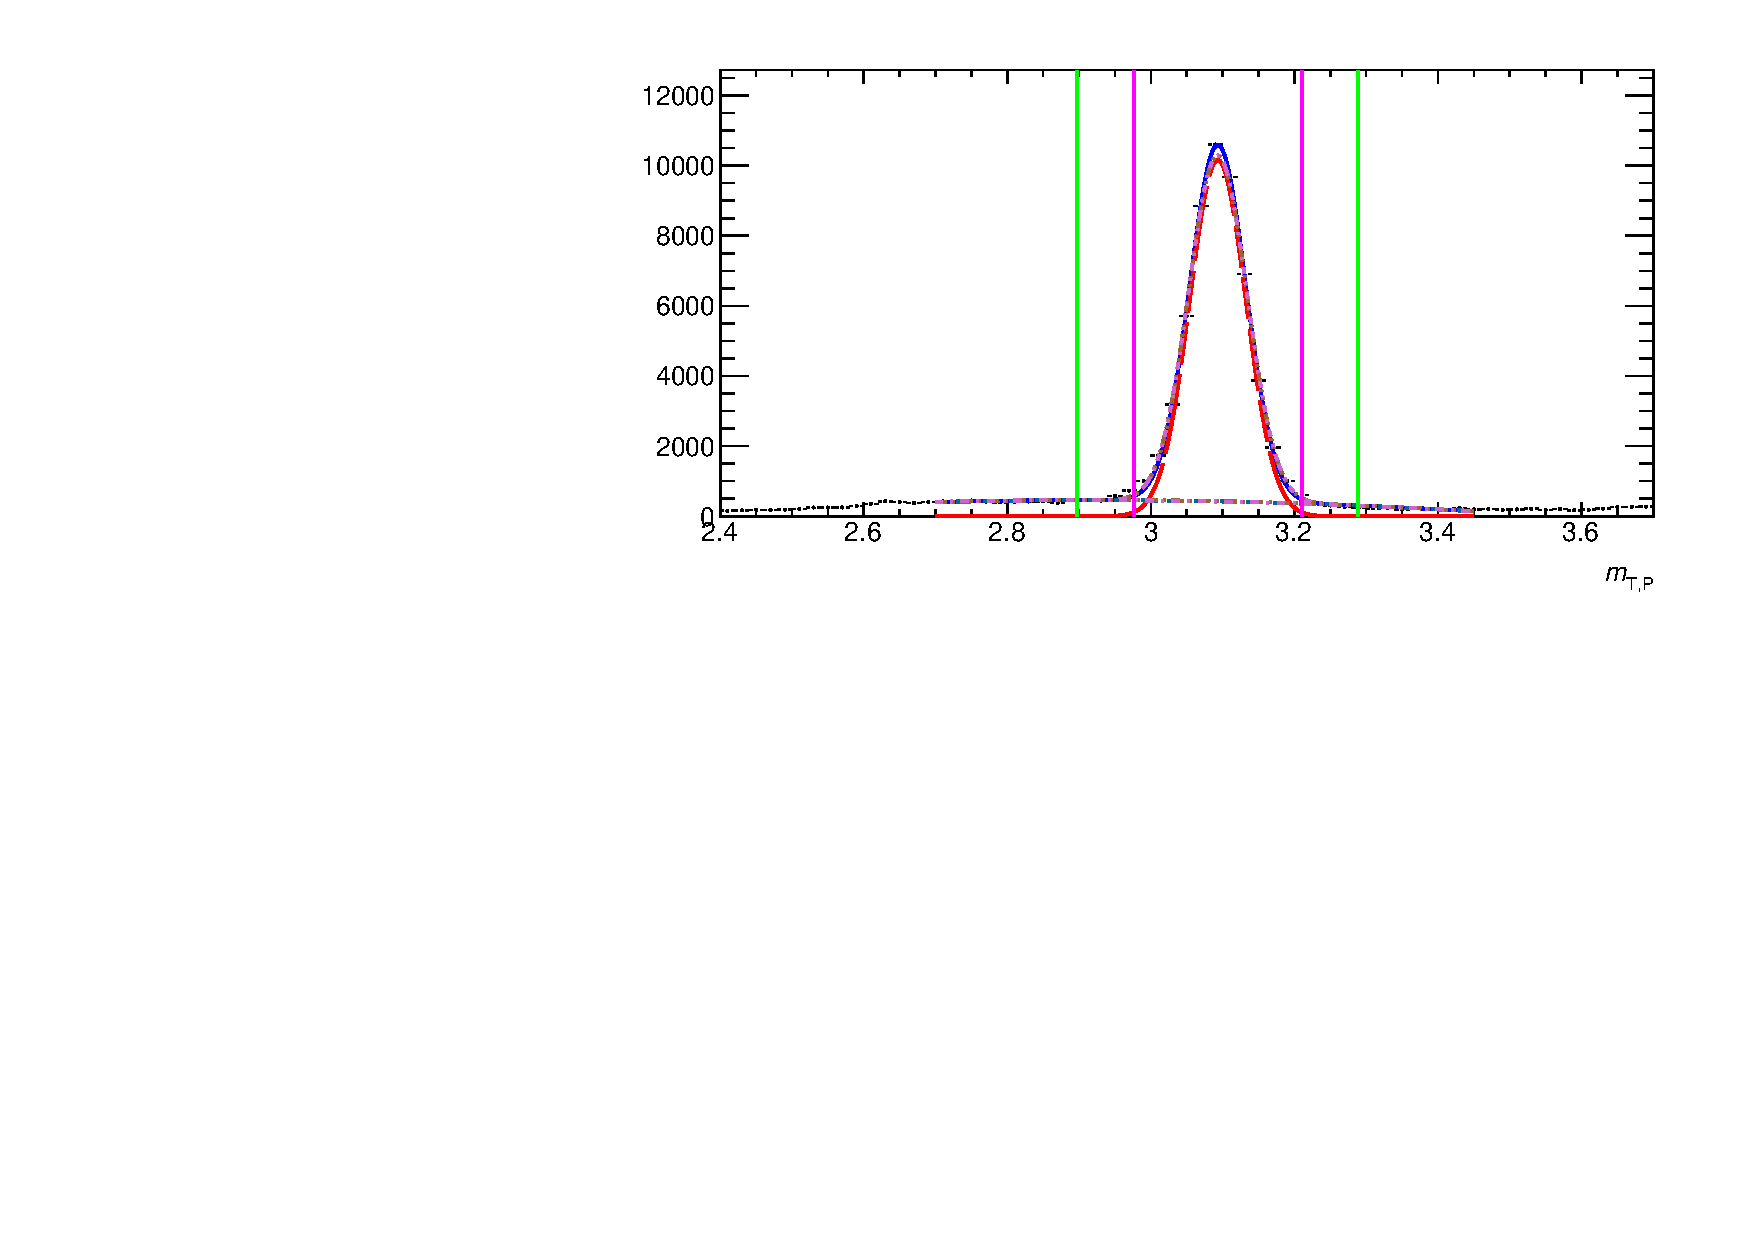
\includegraphics[width=\textwidth]{PartCalibration2012/Plots/Kinematics/Data_InvMass_pt_5_6_barrel_muonprobe.pdf}
      \caption{Muon probe level}   
    \end{subfigure}

    \begin{subfigure}[b]{0.54\textwidth}
      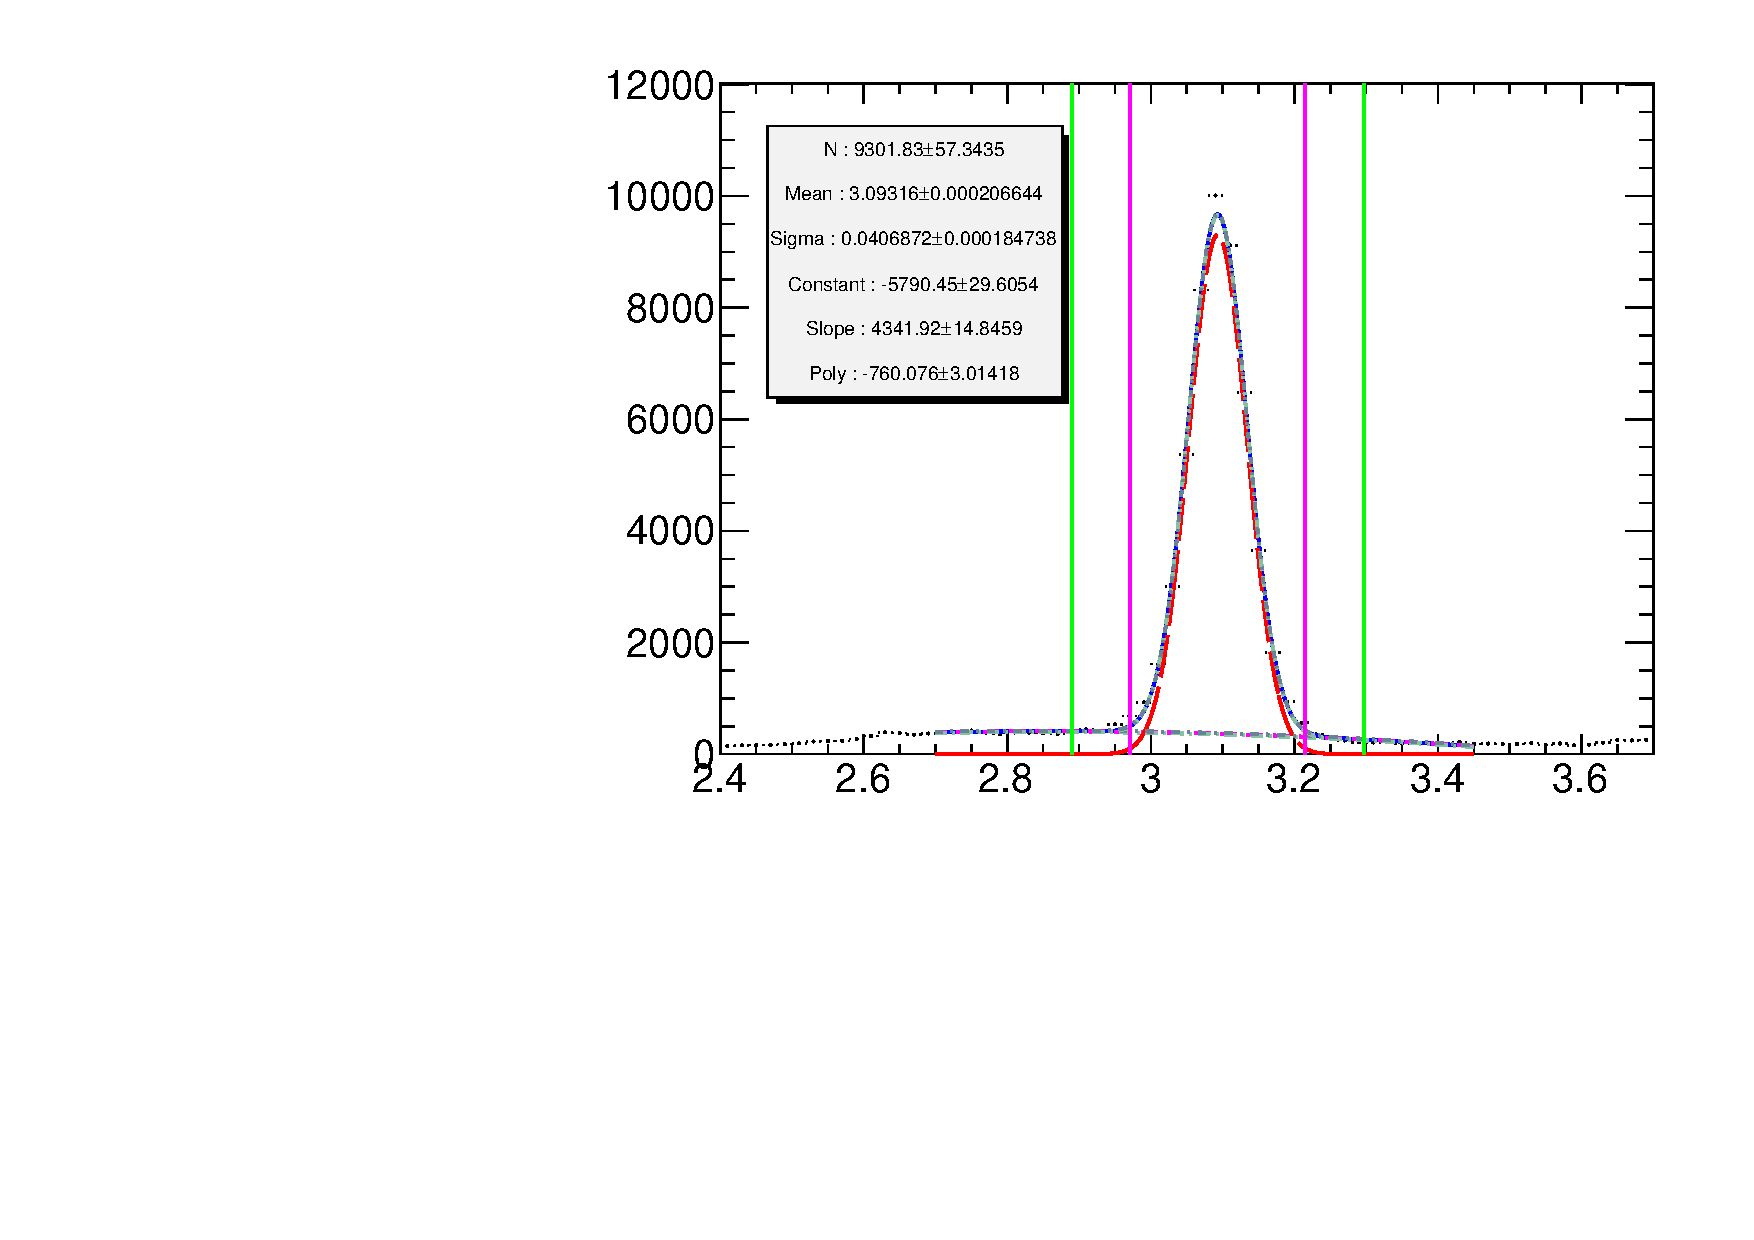
\includegraphics[width=\textwidth]{PartCalibration2012/Plots/Kinematics/Data_InvMass_pt_5_6_barrel_smt.pdf}
      \caption{SMT probe level}   
    \end{subfigure}
    \caption[Invariant mass distributions of tag and probe pairs at probe level, muon probe level, and SMT level in collision data for probes in barrel A with a \pt\ of {\SIrange[range-units=single]{5}{6}{\GeV}}.]{Invariant mass distributions of tag and probe pairs at a) probe level, b) muon probe level, and c) SMT level in collision data for probes in barrel A with a \pt\ of \SIrange[range-units=single]{5}{6}{\GeV}. Shown are all the components of the fit including the variations on the background, and the $3\sigma$ and $5\sigma$ integration windows used for systematics. Fit parameters are shown with uncertainties.}\label{fig:CalibrationFittingResult}
\end{figure}

\section{Efficiencies}\label{sec:CalibrationEfficiencies}

The efficiency is monitored as a function of a variety of kinematic variables, including the isolation, transverse momentum, azimuthal angle, and the pseudorapidity of the probe.

\subsection{The 2011 calibration}

The selection and fitting procedure used for this calibration are based on the 2011 analysis~\cite{Calibration:MattThesis}. In that calibration, the efficiencies measured exhibited no dependence on $\phi$, an asymmetric dependence on $\eta$ particularly in the forward regions of the detector, and a dependence on \pt. The scale factors were consistent with unity within their uncertainty across the entire $\eta$ and $\pt$ range examined as shown in Table~\ref{tab:Calibration2011SF}.

\begin{table}[bhtp]
  \centering
  \tabcolsep=0.11cm
  \ra{1.3}
  \sisetup{range-phrase=--}
  \begin{tabular}{@{}%
                    l%
                    *{5}{S[table-format=1.3(3)]}%
                    @{}}
    \toprule
    \pt\ range [\si{\GeV}]   & \multicolumn{5}{c}{Scale Factor in} \\
    \midrule
    \textbf{Side A}          & {Crack}   & {Barrel} & {Transition} & {End-cap} & {Forward} \\
    \tabin\numrange{4}{5}   & 0.974(9)  & 0.981(3) & 0.987(7)     & 0.981(3) & 0.991(5)  \\
    \tabin\numrange{5}{6}   & 0.996(8)  & 0.983(3) & 0.987(8)     & 0.988(4) & 0.980(6)  \\
    \tabin\numrange{6}{7}   & 0.990(9)  & 0.984(3) & 0.960(10)    & 0.984(5) & 0.981(6)  \\
    \tabin\numrange{7}{8}   & 0.966(13) & 0.987(4) & 0.978(8)     & 0.990(6) & 0.982(7)  \\
    \tabin\numrange{8}{10}  & 0.983(11) & 0.981(3) & 1.005(9)     & 0.988(5) & 0.954(8)  \\
    \tabin\numrange{10}{12} & 0.928(19) & 0.979(4) & 1.002(9)     & 0.991(6) & 0.984(11) \\
    \midrule
    \textbf{Side C}          & {Crack}   & {Barrel} & {Transition} & {End-cap} & {Forward} \\
    \tabin\numrange{4}{5}   & 0.984(8)  & 0.978(3) & 0.992(7)     & 0.979(3) & 1.005(6)  \\
    \tabin\numrange{5}{6}   & 0.992(7)  & 0.991(2) & 0.982(9)     & 0.986(4) & 1.012(7)  \\
    \tabin\numrange{6}{7}   & 0.989(8)  & 0.981(3) & 0.980(8)     & 0.990(5) & 1.003(10) \\
    \tabin\numrange{7}{8}   & 0.931(17) & 0.983(3) & 0.970(53)    & 0.985(6) & 1.047(10) \\
    \tabin\numrange{8}{10}  & 0.981(17) & 0.987(3) & 0.968(9)     & 0.990(5) & 1.100(8)  \\
    \tabin\numrange{10}{12} & 0.974(15) & 0.976(4) & 0.970(11)    & 1.002(6) & 1.083(10) \\
    \bottomrule
  \end{tabular}
  \caption[Data/MC Scale Factors for 2011 Data in all five regions of the detector as a function of \pt.]{Data/MC Scale Factors for 2011 Data in all five regions of the detector as a function of \pt. The uncertainties include systematic and statistical components as described in~\cite{Calibration:MattThesis}.}\label{tab:Calibration2011SF}
\end{table}

\subsection{Efficiency binning}
\sisetup{range-phrase=--}
The binning in most variables is governed by the amount of statistics required to produce stable, good quality fits. The binning in pseudorapidity, summarized in Table~\ref{tab:CalibrationEtaRegions}, corresponds with different regions of the ATLAS detector and differentiates between the positive and negative sides. The chosen \pt\ binning is shown in Table~\ref{tab:Calibration2012SF}.

\begin{table}[thbp]
  \centering
  \begin{tabular}{@{}lc@{}}
    \toprule
    Name       & $|\eta|$ range \\
    \midrule
    Crack      & \numrange{0.0}{0.1} \\
    Barrel     & \numrange{0.1}{1.1} \\
    Transition & \numrange{1.1}{1.3} \\
    End-cap    & \numrange{1.3}{2.0} \\
    Forward    & \numrange{2.0}{2.5} \\
    \bottomrule
  \end{tabular}
  \caption{Pseudorapidity regions of the ATLAS detector.}\label{tab:CalibrationEtaRegions}
\end{table}

\section{Results}

The reconstruction and \xsm\ tagging efficiencies are presented in the following pages as a function of $\eta$, $\phi$ and \pt. The STACO CB reconstruction efficiencies and scale factors as measured in side A and C of the detector are shown in Figure~\ref{fig:RecoEffSideA} and Figure~\ref{fig:RecoEffSideC} respectively. The efficiencies exhibit a strong dependence on transverse momentum and pseudorapidity.

The reconstruction efficiency for muons in the crack region appears to suffer from low statistics particularly in the high-\pt\ range, this is expected due to the MS being only partially equipped in the region around $\eta=0$. In the transition region the MS coverage in $\phi$ is not uniform due to some chambers not being installed.

It is important to note that the nominal calibration of the reconstruction efficiency within ATLAS is performed on \ZMu\ due to the smaller uncertainty using high \pt\ muons. The SF at low \pt\ are obtained by extrapolating back into the low momentum range.

\begin{figure}[htbp]
  \centering
    \begin{subfigure}[b]{0.45\textwidth}
      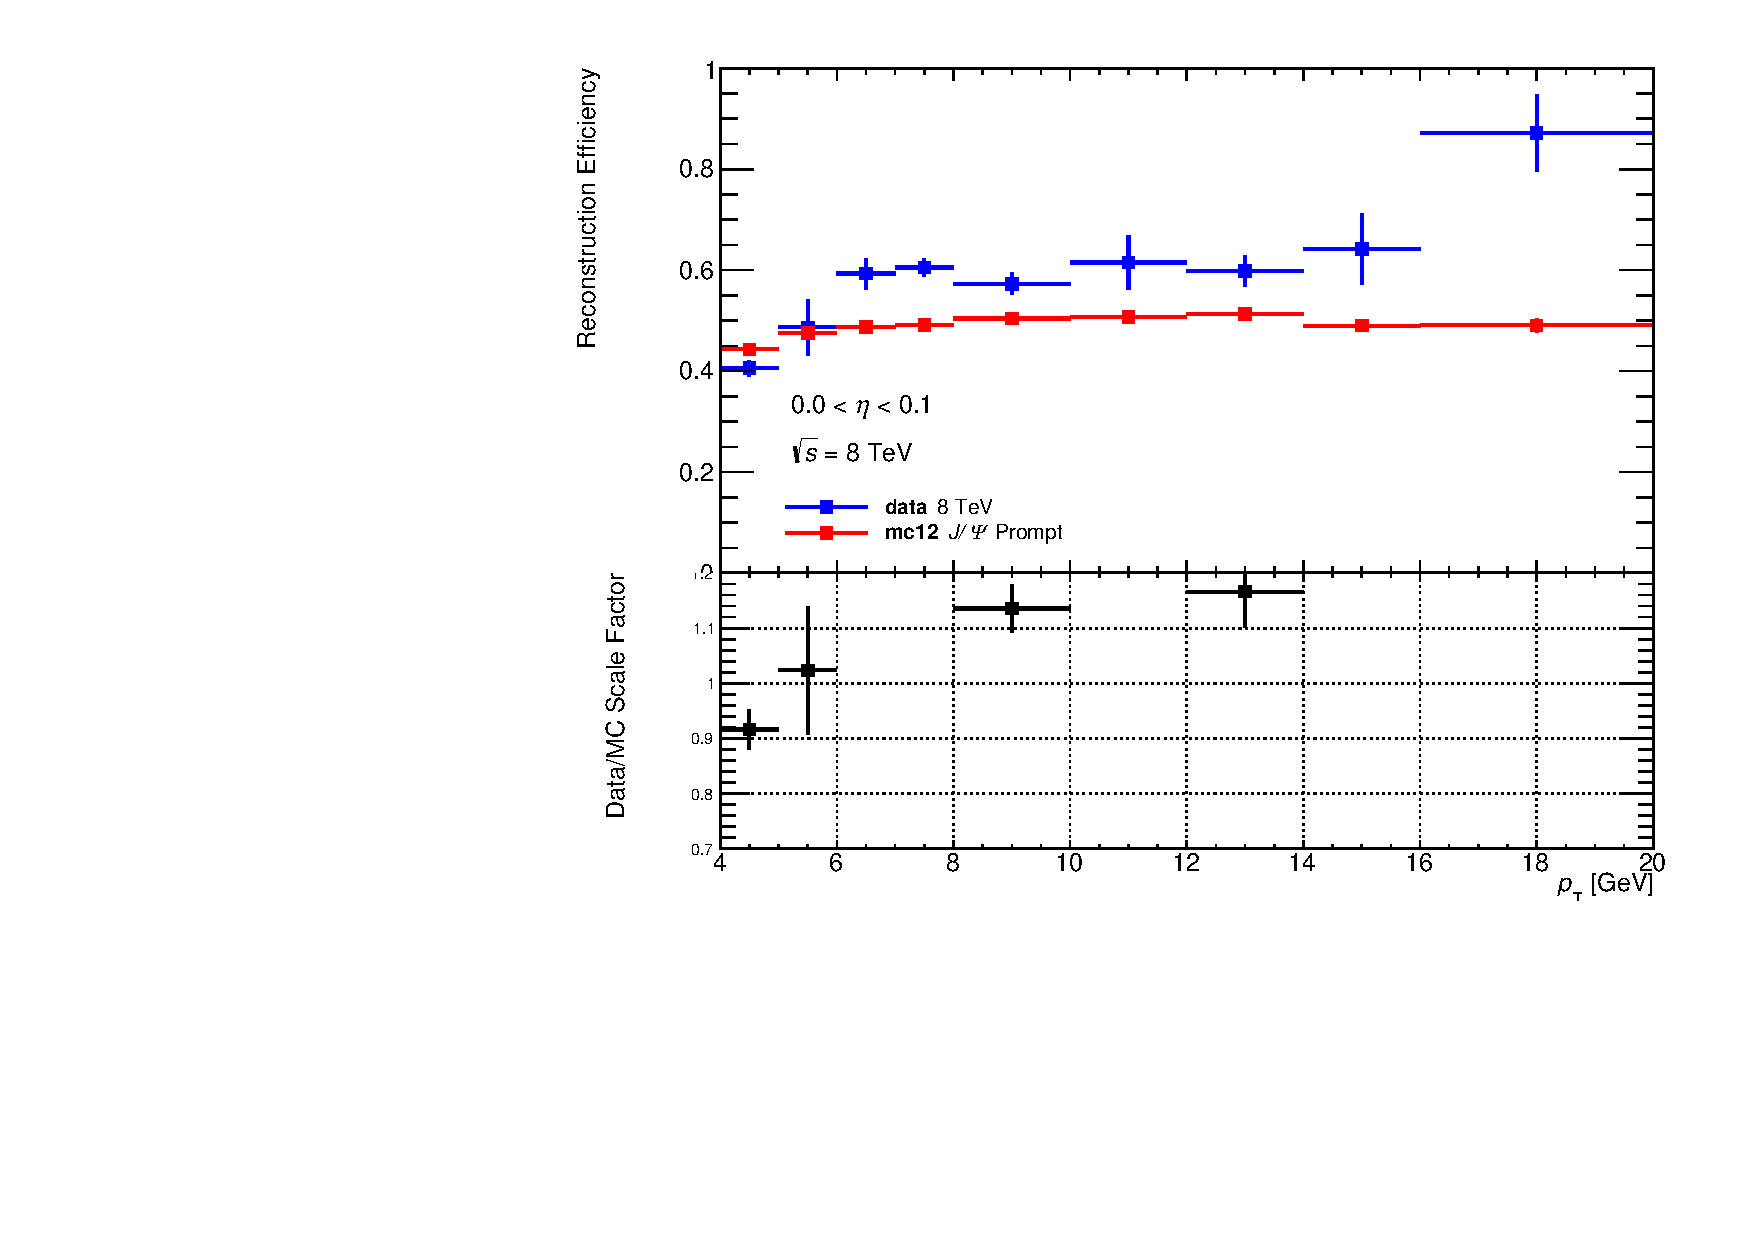
\includegraphics[width=\textwidth]{PartCalibration2012/Plots/SFPlots/Crack_A_reco.pdf}
      \caption{Crack A.}\label{fig:CalibrationRecoSFCrackA}
    \end{subfigure}
    \hfill
    \begin{subfigure}[b]{0.45\textwidth}
      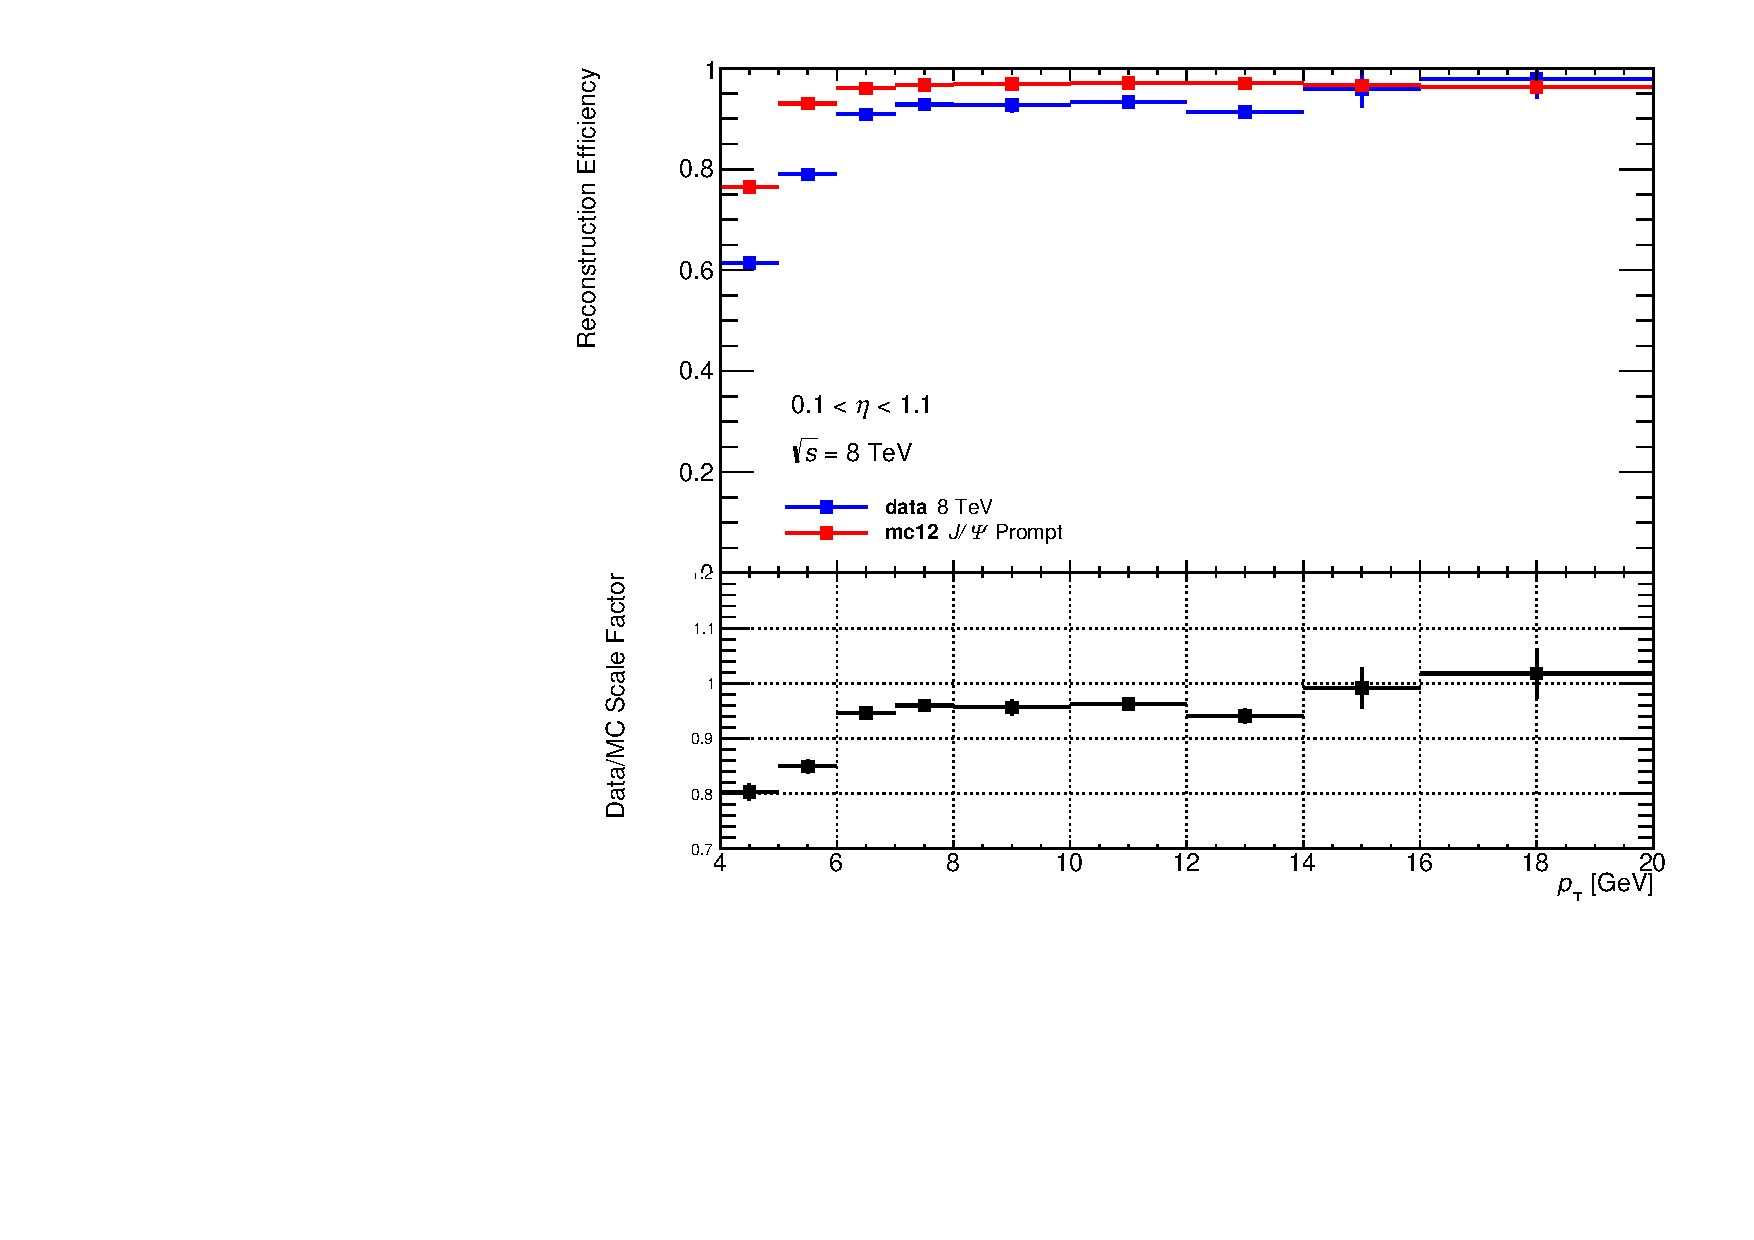
\includegraphics[width=\textwidth]{PartCalibration2012/Plots/SFPlots/Barrel_A_reco.pdf}
      \caption{Barrel A.}\label{fig:CalibrationRecoSFBarrelA}
    \end{subfigure}

    \begin{subfigure}[b]{0.45\textwidth}
      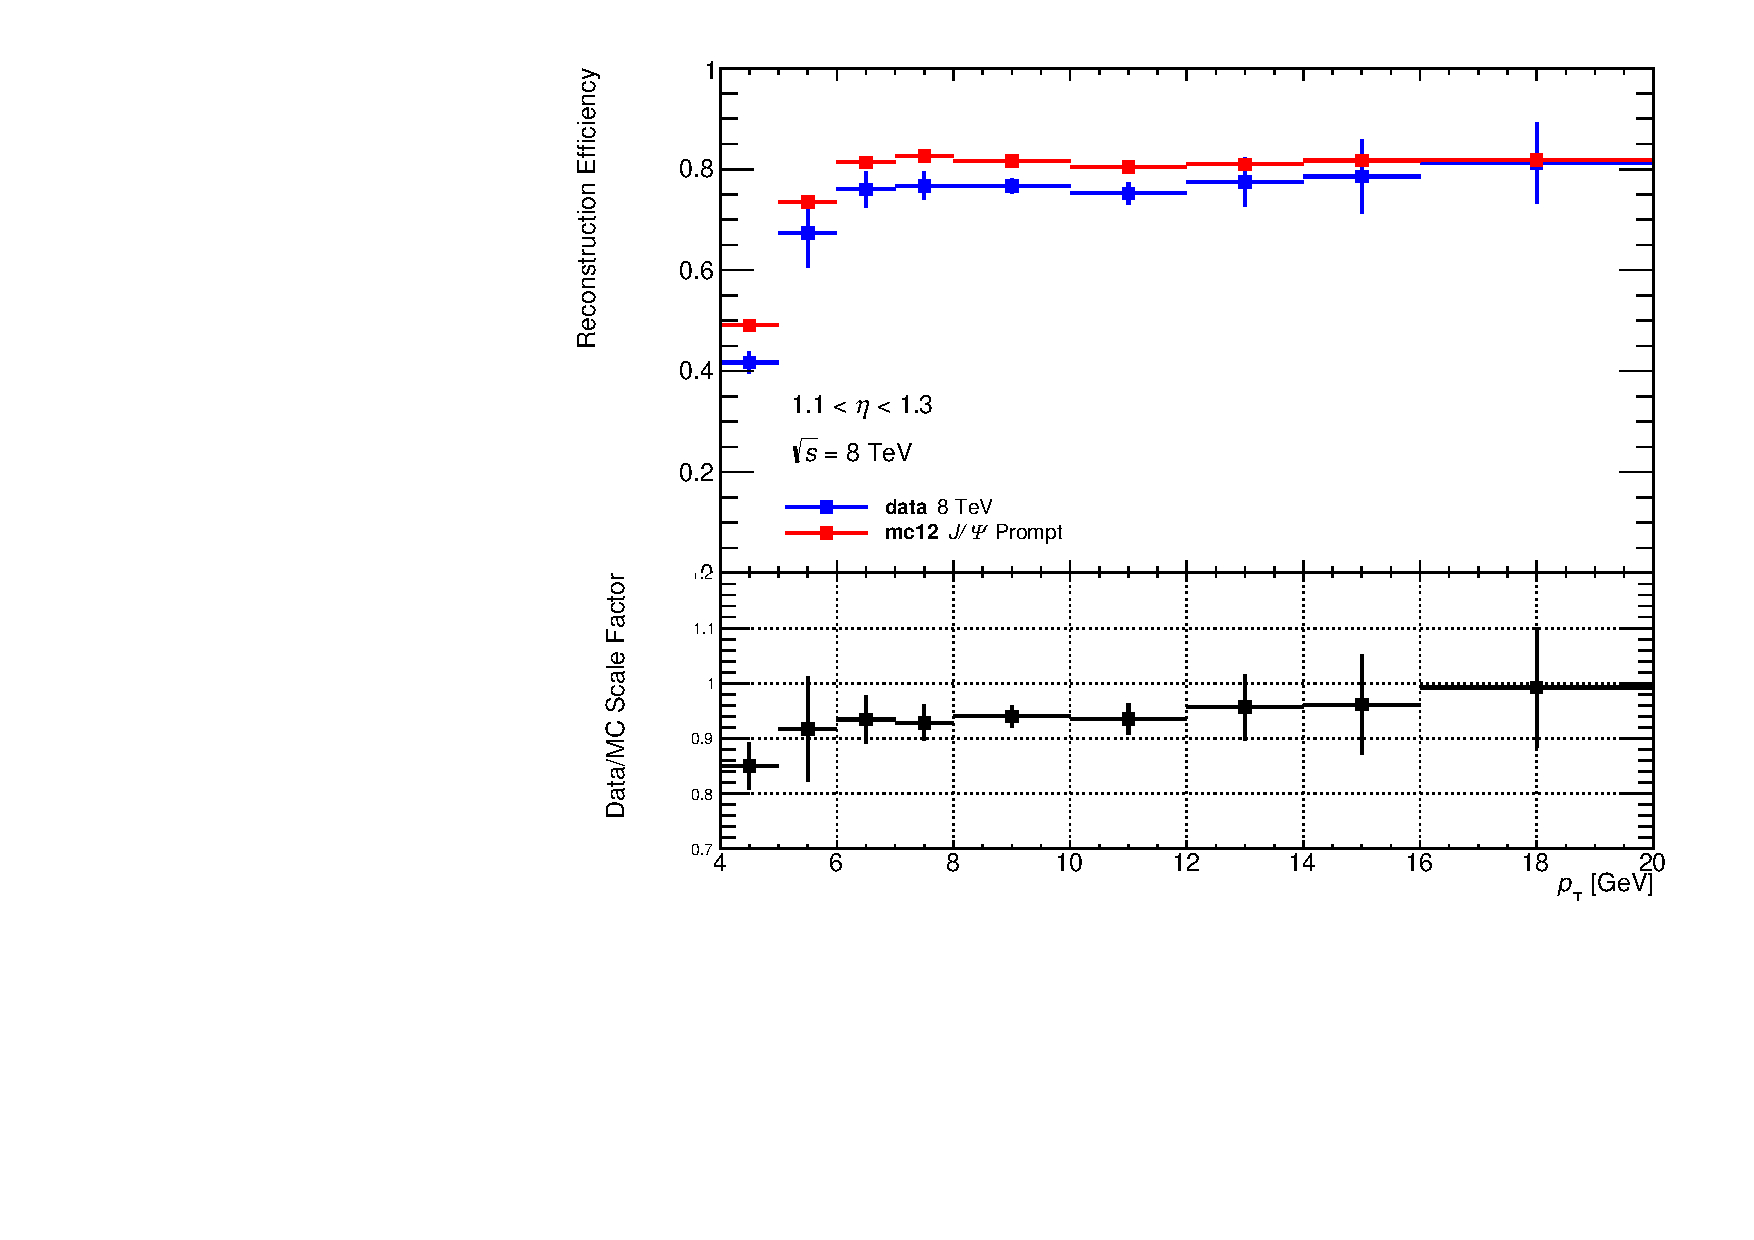
\includegraphics[width=\textwidth]{PartCalibration2012/Plots/SFPlots/Transition_A_reco.pdf}
      \caption{Transition A.}\label{fig:CalibrationRecoSFTransitionA}
    \end{subfigure}
    \hfill
    \begin{subfigure}[b]{0.45\textwidth}
      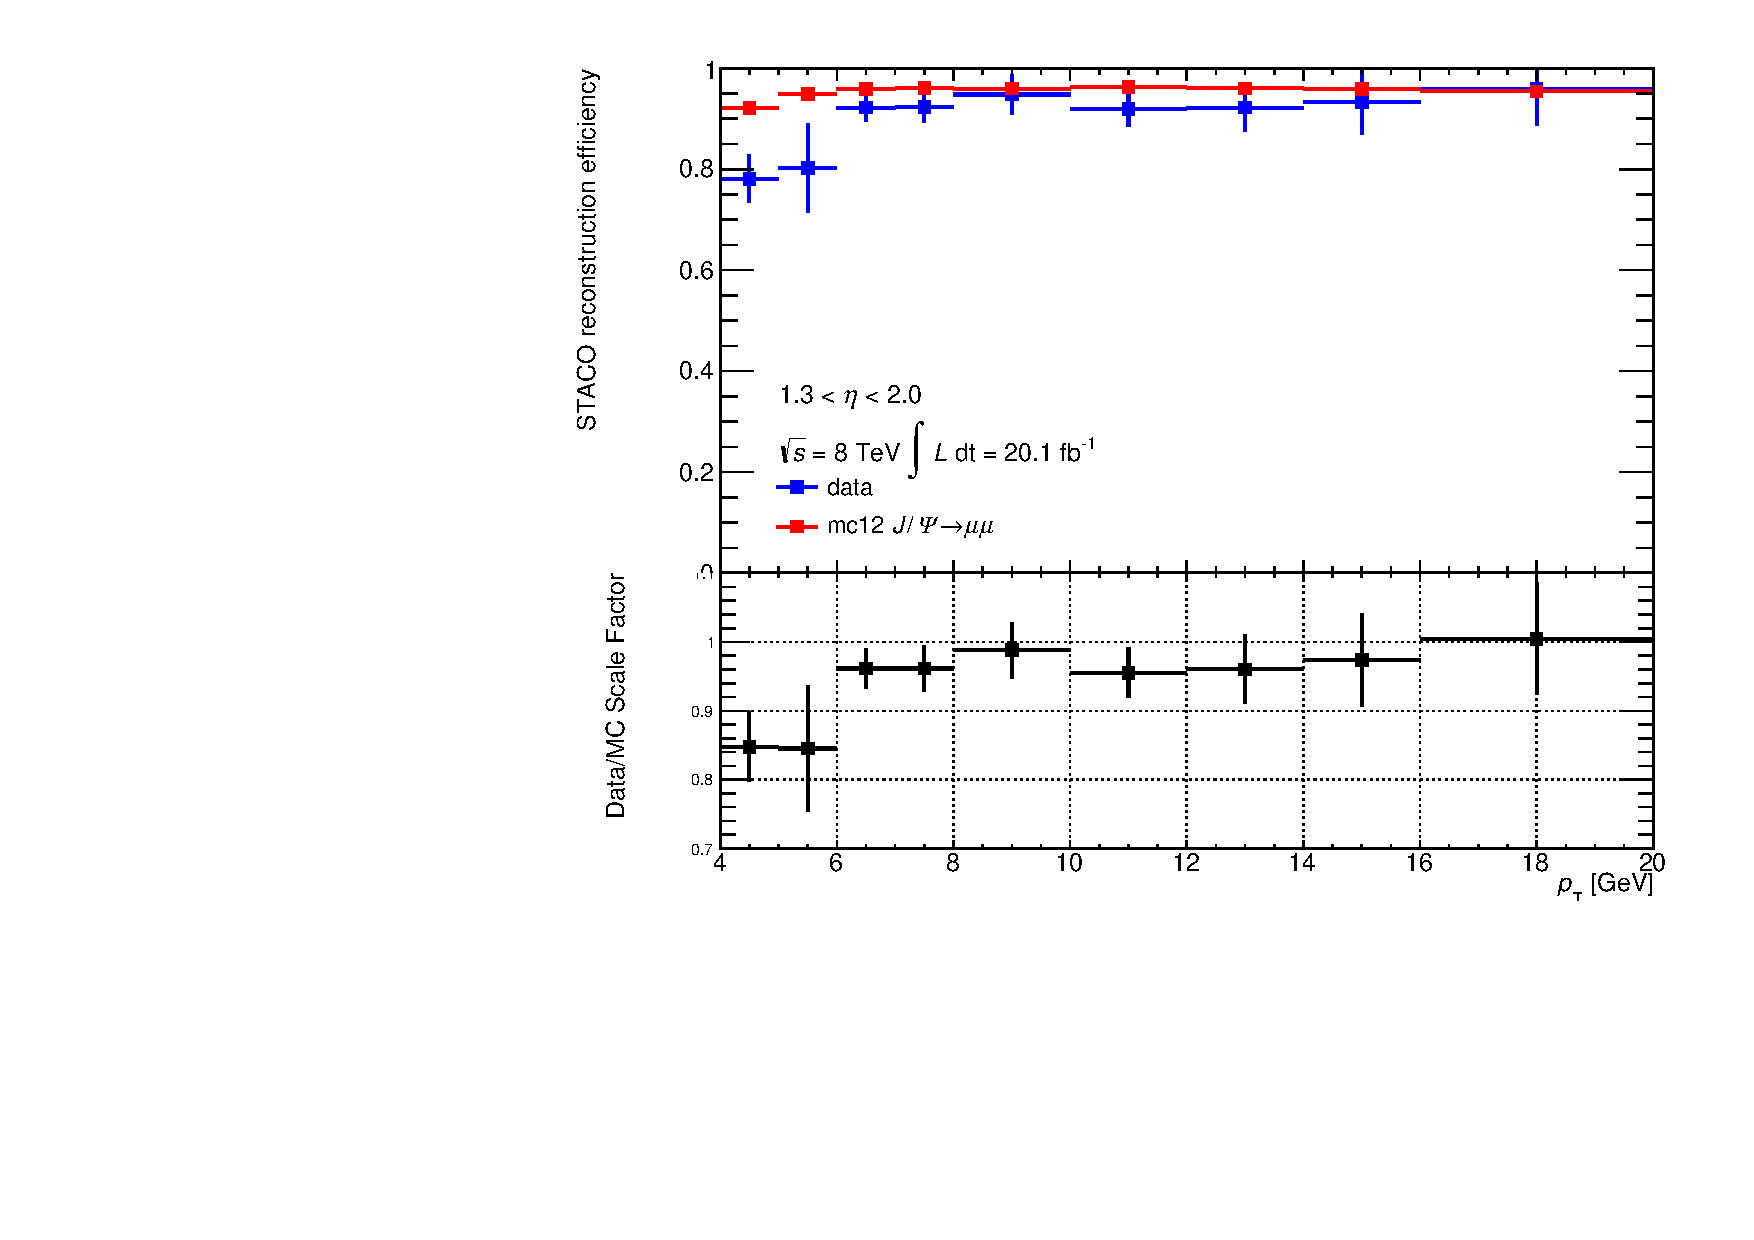
\includegraphics[width=\textwidth]{PartCalibration2012/Plots/SFPlots/Endcap_A_reco.pdf}
      \caption{End-cap A.}\label{fig:CalibrationRecoSFEndcapA}
    \end{subfigure}

    \begin{subfigure}[b]{0.45\textwidth}
      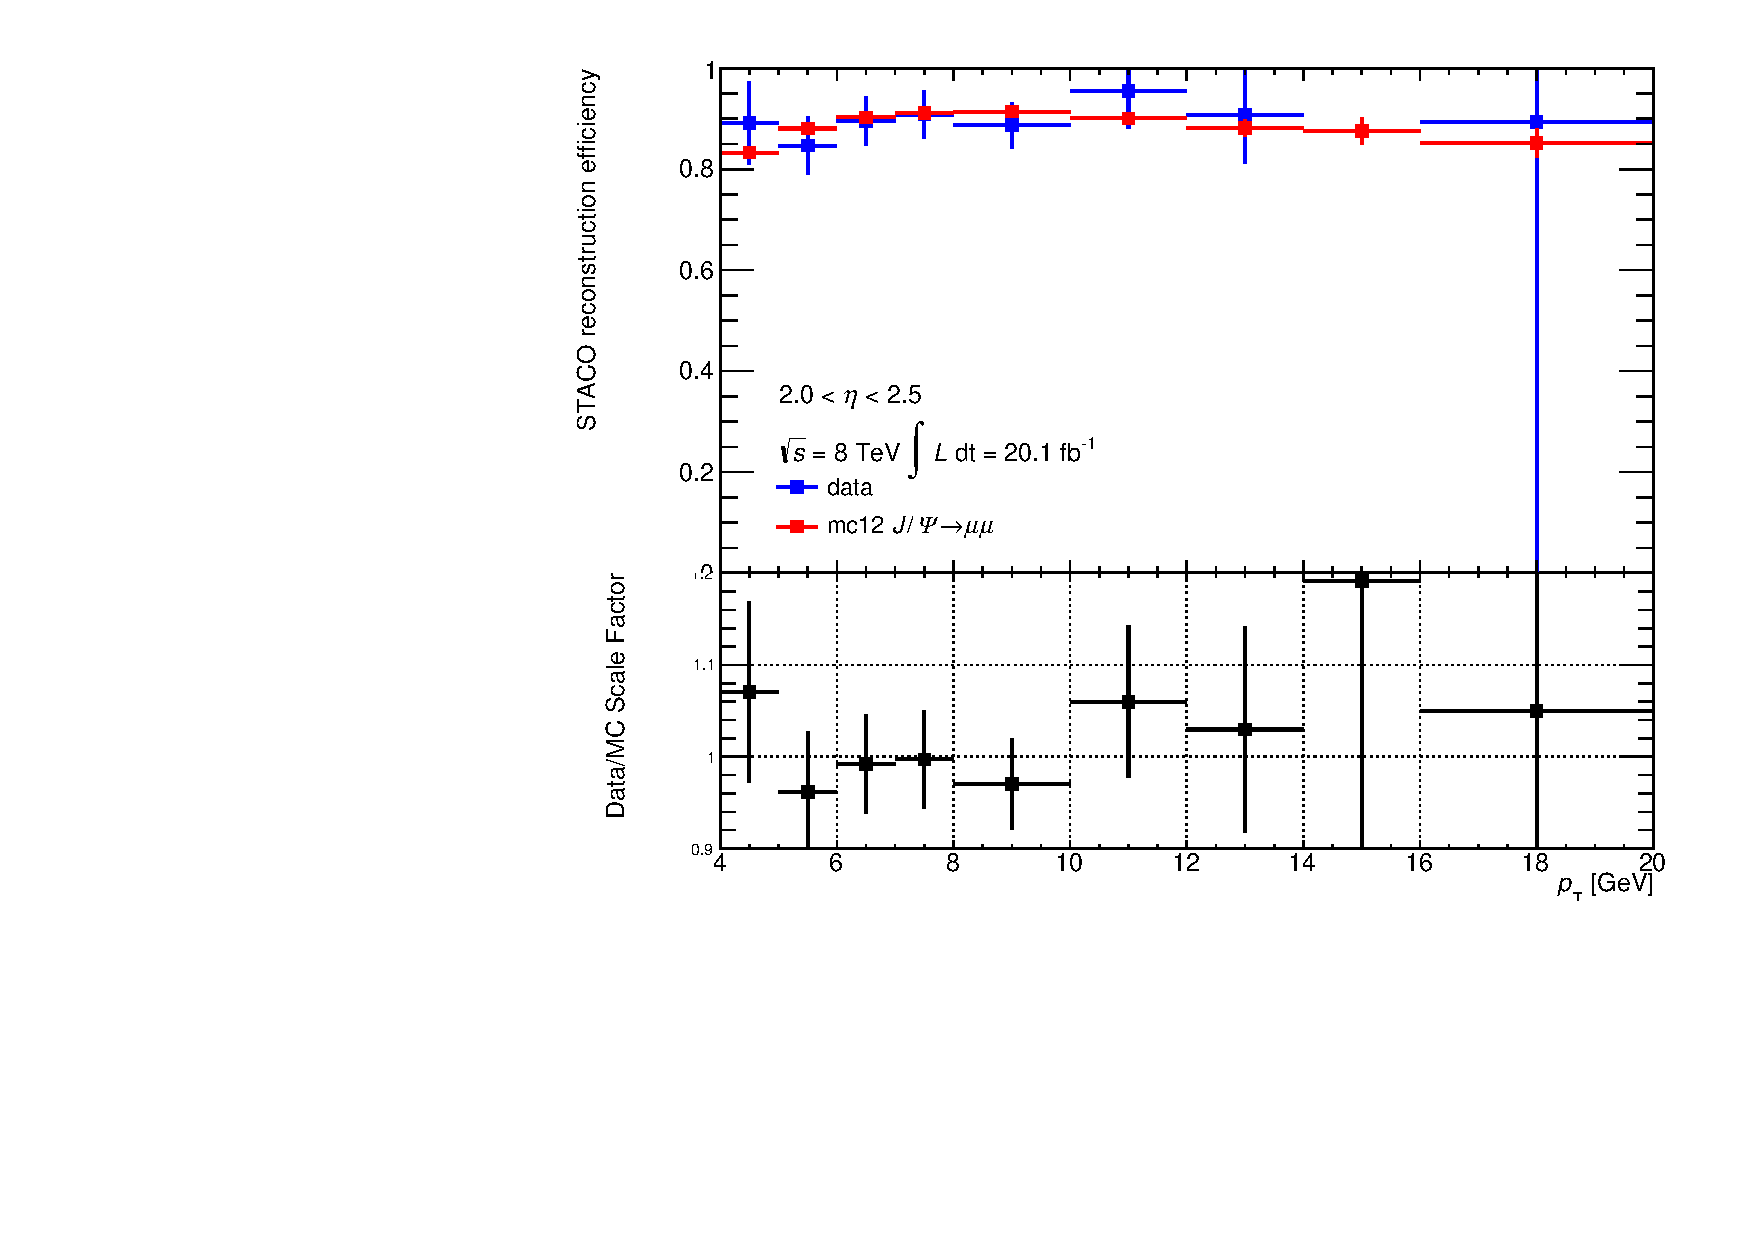
\includegraphics[width=\textwidth]{PartCalibration2012/Plots/SFPlots/Forward_A_reco.pdf}
      \caption{Forward A.}\label{fig:CalibrationRecoSFForwardA}
    \end{subfigure}
    \caption{Distribution of the STACO CB reconstruction efficiency as measured in data and MC, and the associated scale factor as a function of the probe \pt\ measured in side A for all detector regions.}\label{fig:RecoEffSideA}
\end{figure}

\begin{figure}[htbp]
  \centering
    \begin{subfigure}[b]{0.45\textwidth}
      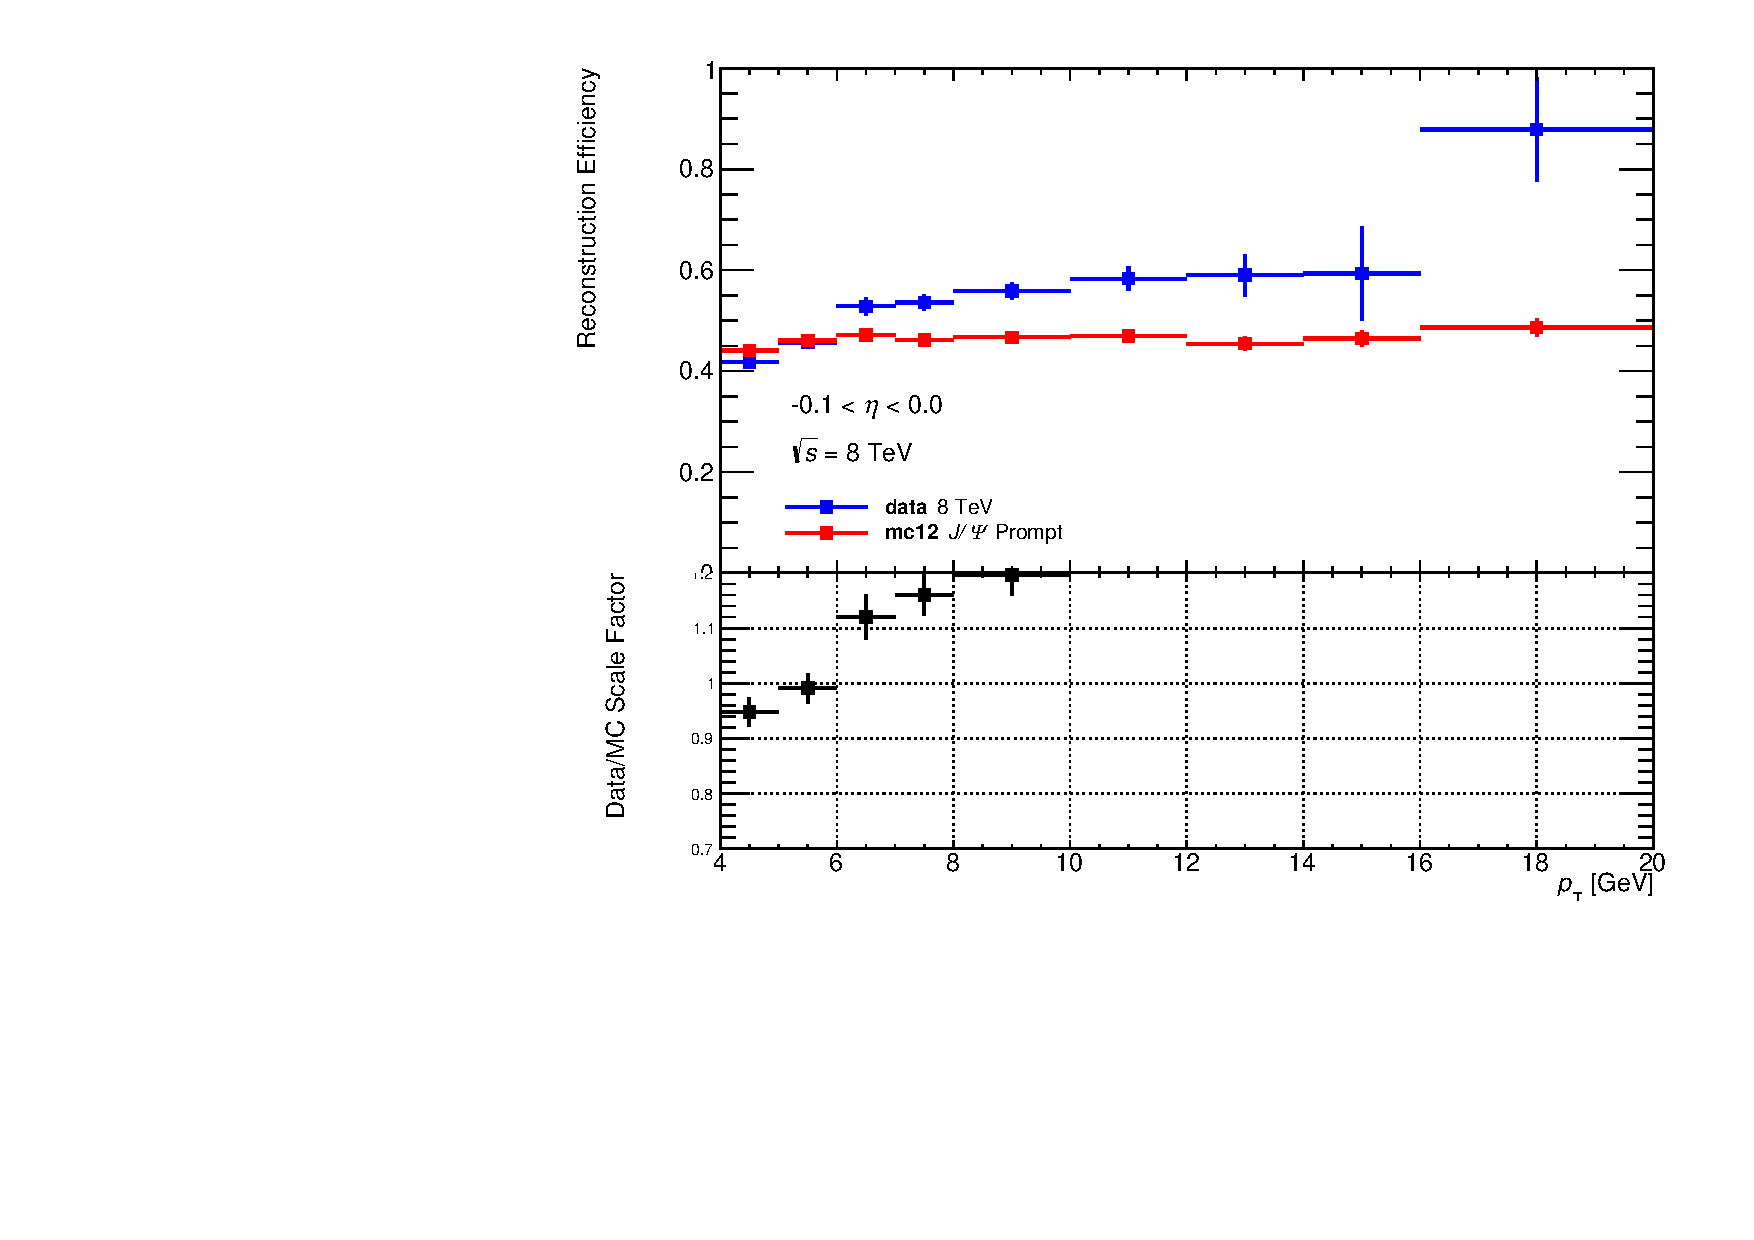
\includegraphics[width=\textwidth]{PartCalibration2012/Plots/SFPlots/Crack_C_reco.pdf}
      \caption{Crack C.}\label{fig:CalibrationRecoSFCrackC}
    \end{subfigure}
    \hfill
    \begin{subfigure}[b]{0.45\textwidth}
      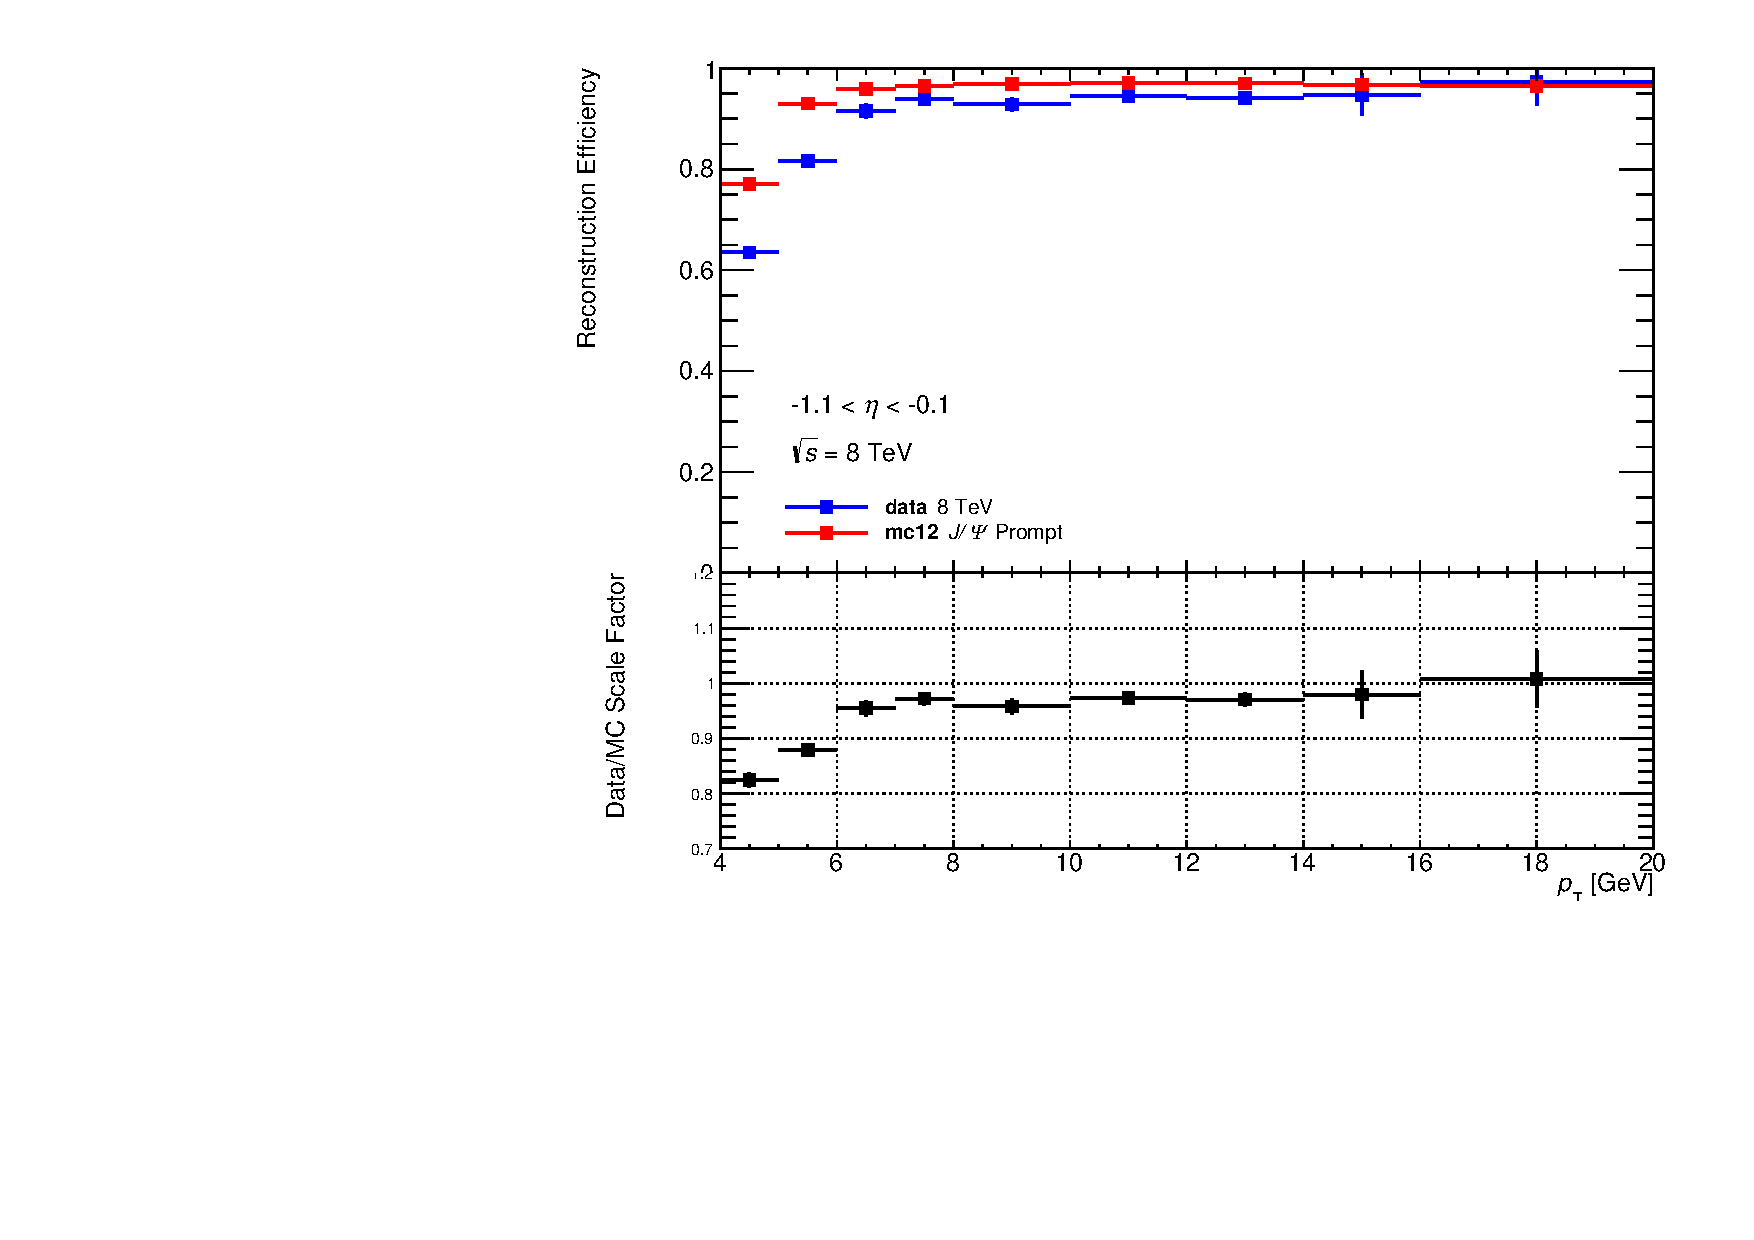
\includegraphics[width=\textwidth]{PartCalibration2012/Plots/SFPlots/Barrel_C_reco.pdf}
      \caption{Barrel C.}\label{fig:CalibrationRecoSFBarrelC}
    \end{subfigure}

    \begin{subfigure}[b]{0.45\textwidth}
      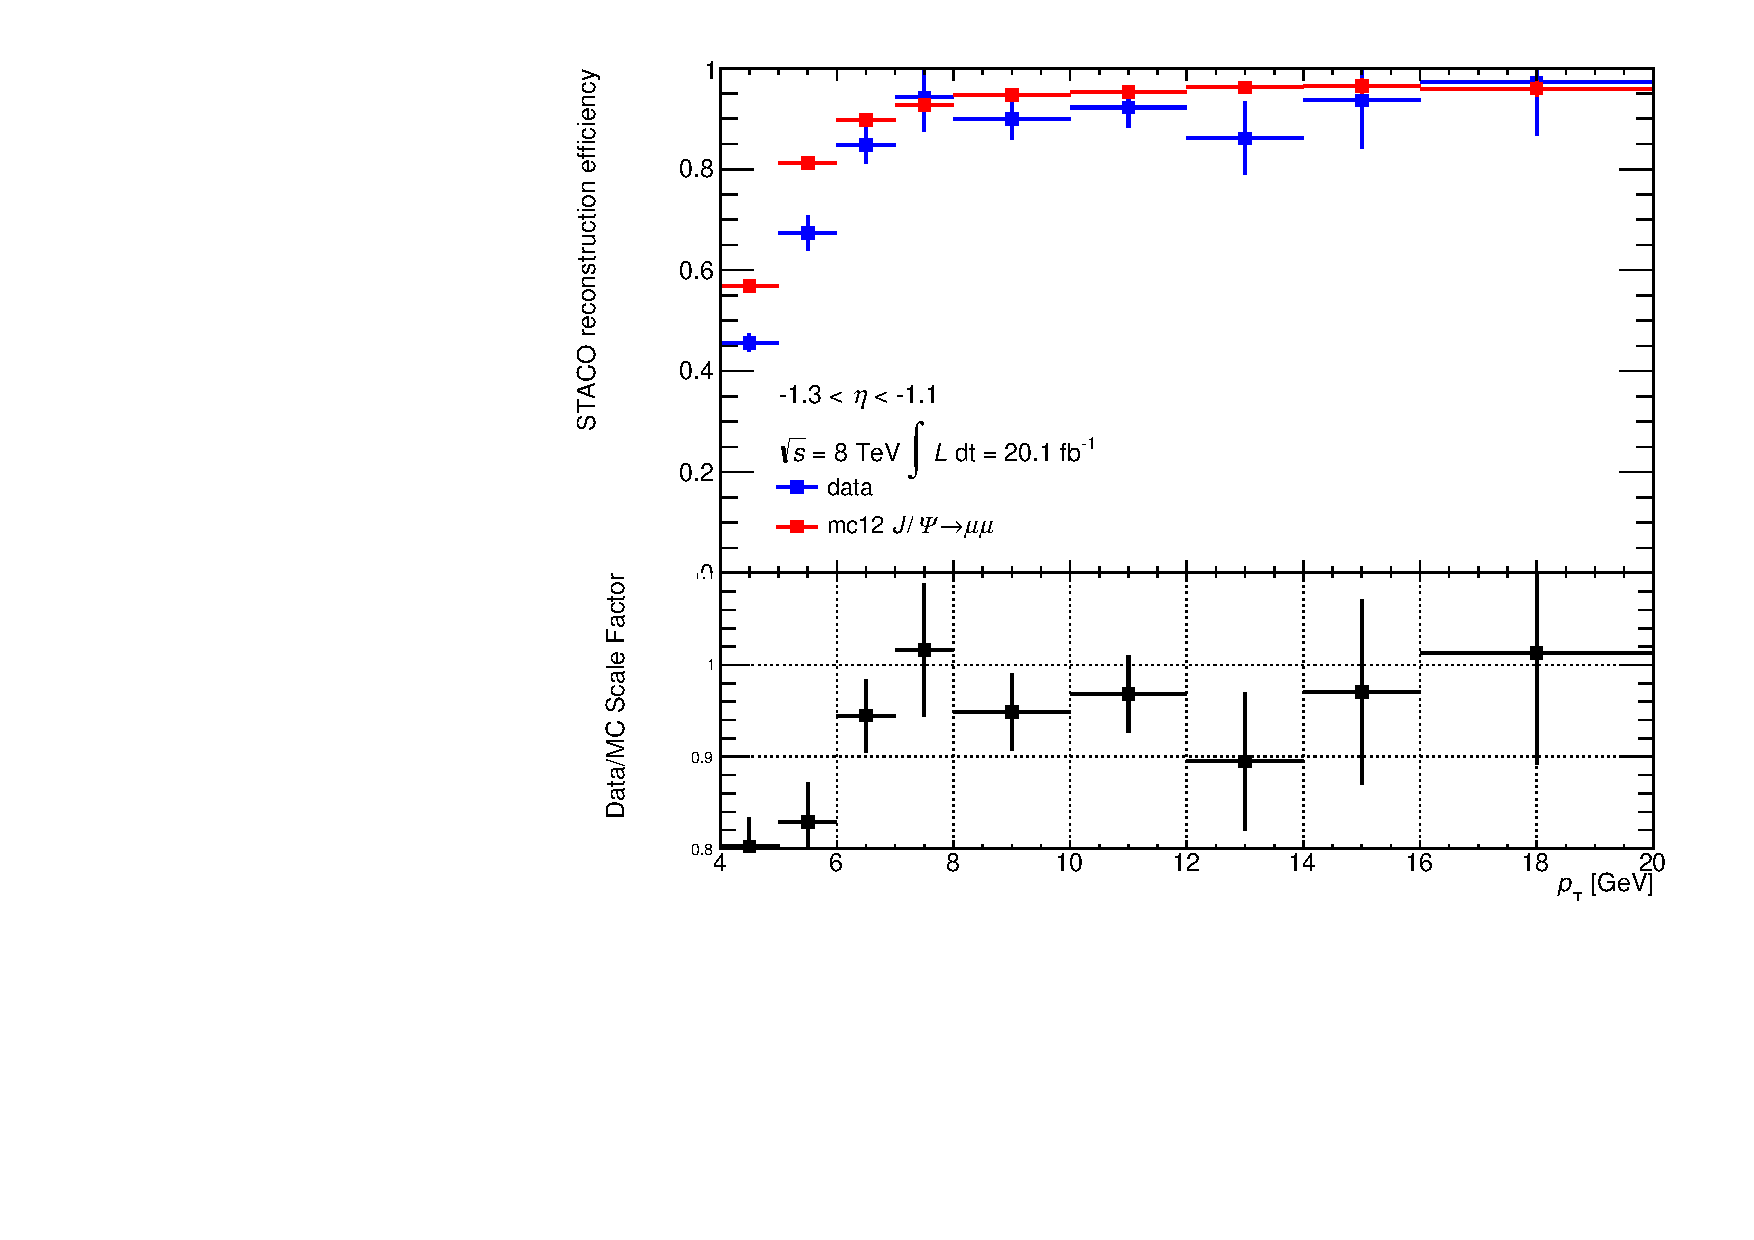
\includegraphics[width=\textwidth]{PartCalibration2012/Plots/SFPlots/Transition_C_reco.pdf}
      \caption{Transition C.}\label{fig:CalibrationRecoSFTransitionC}
    \end{subfigure}
    \hfill
    \begin{subfigure}[b]{0.45\textwidth}
      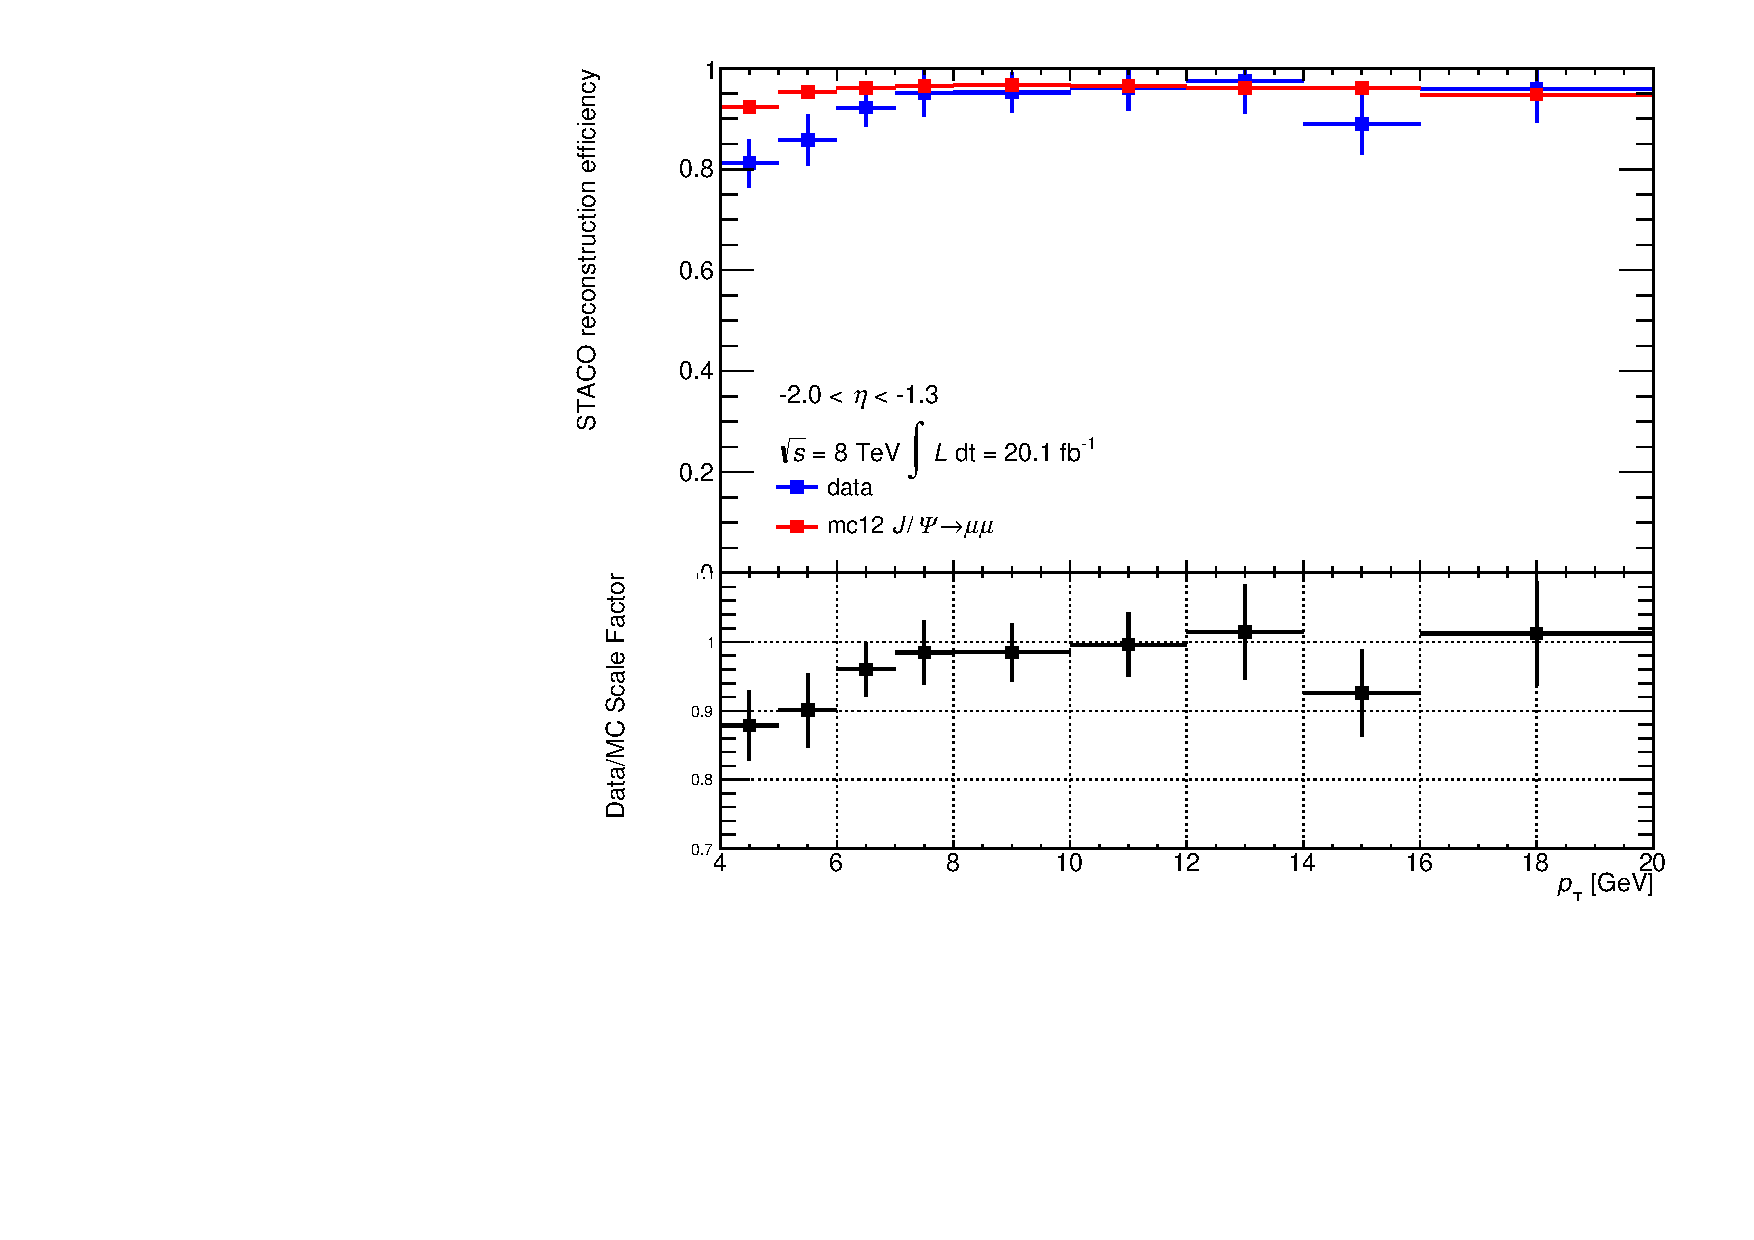
\includegraphics[width=\textwidth]{PartCalibration2012/Plots/SFPlots/Endcap_C_reco.pdf}
      \caption{End-cap C.}\label{fig:CalibrationRecoSFEndcapC}
    \end{subfigure}

    \begin{subfigure}[b]{0.45\textwidth}
      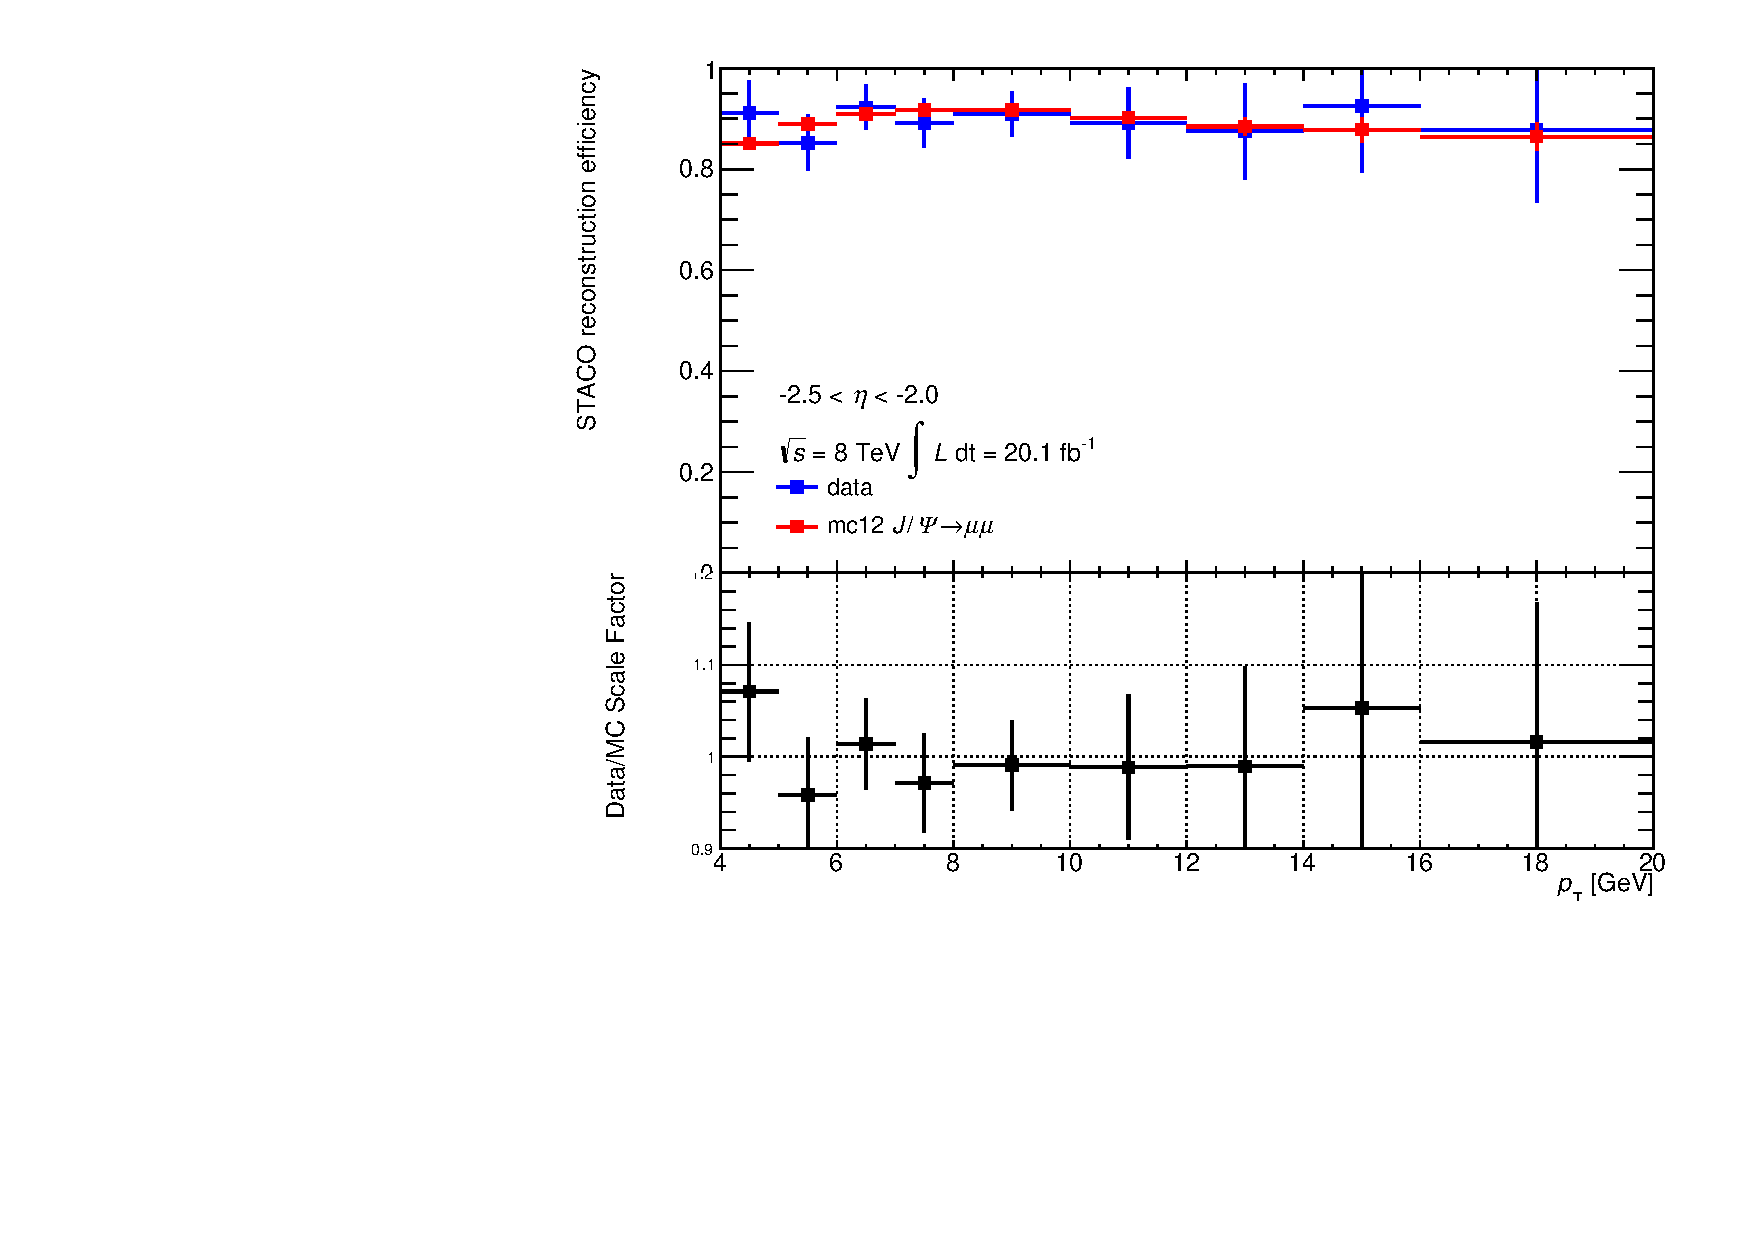
\includegraphics[width=\textwidth]{PartCalibration2012/Plots/SFPlots/Forward_C_reco.pdf}
      \caption{Forward C.}\label{fig:CalibrationRecoSFForwardC}
    \end{subfigure}
    \caption{Distribution of the STACO CB reconstruction efficiency as measured in data and MC, and the associated scale factor as a function of the probe \pt\ measured in side C for all detector regions.}\label{fig:RecoEffSideC}
\end{figure}

The \xsm\ tagging efficiency exhibits an asymmetric dependence on the muon probe pseudorapidity, but no dependence on the azimuthal angle $\phi$ (Figure~\ref{fig:CalibrationAngularResults}). As expected, there is a strong dependence on the transverse momentum of the muon probe (Figure~\ref{fig:CalibrationMomentumResults}). As in the 2011 analysis it was decided to bin the SF as a function of \pt\ and $\eta$, distinguishing between side A and C of the detector. The scale factor and efficiency distributions are presented in the next pages. 

% SF vs Eta, Phi
\begin{figure}[htbp]
  \centering
  \begin{subfigure}[b]{0.75\textwidth}
      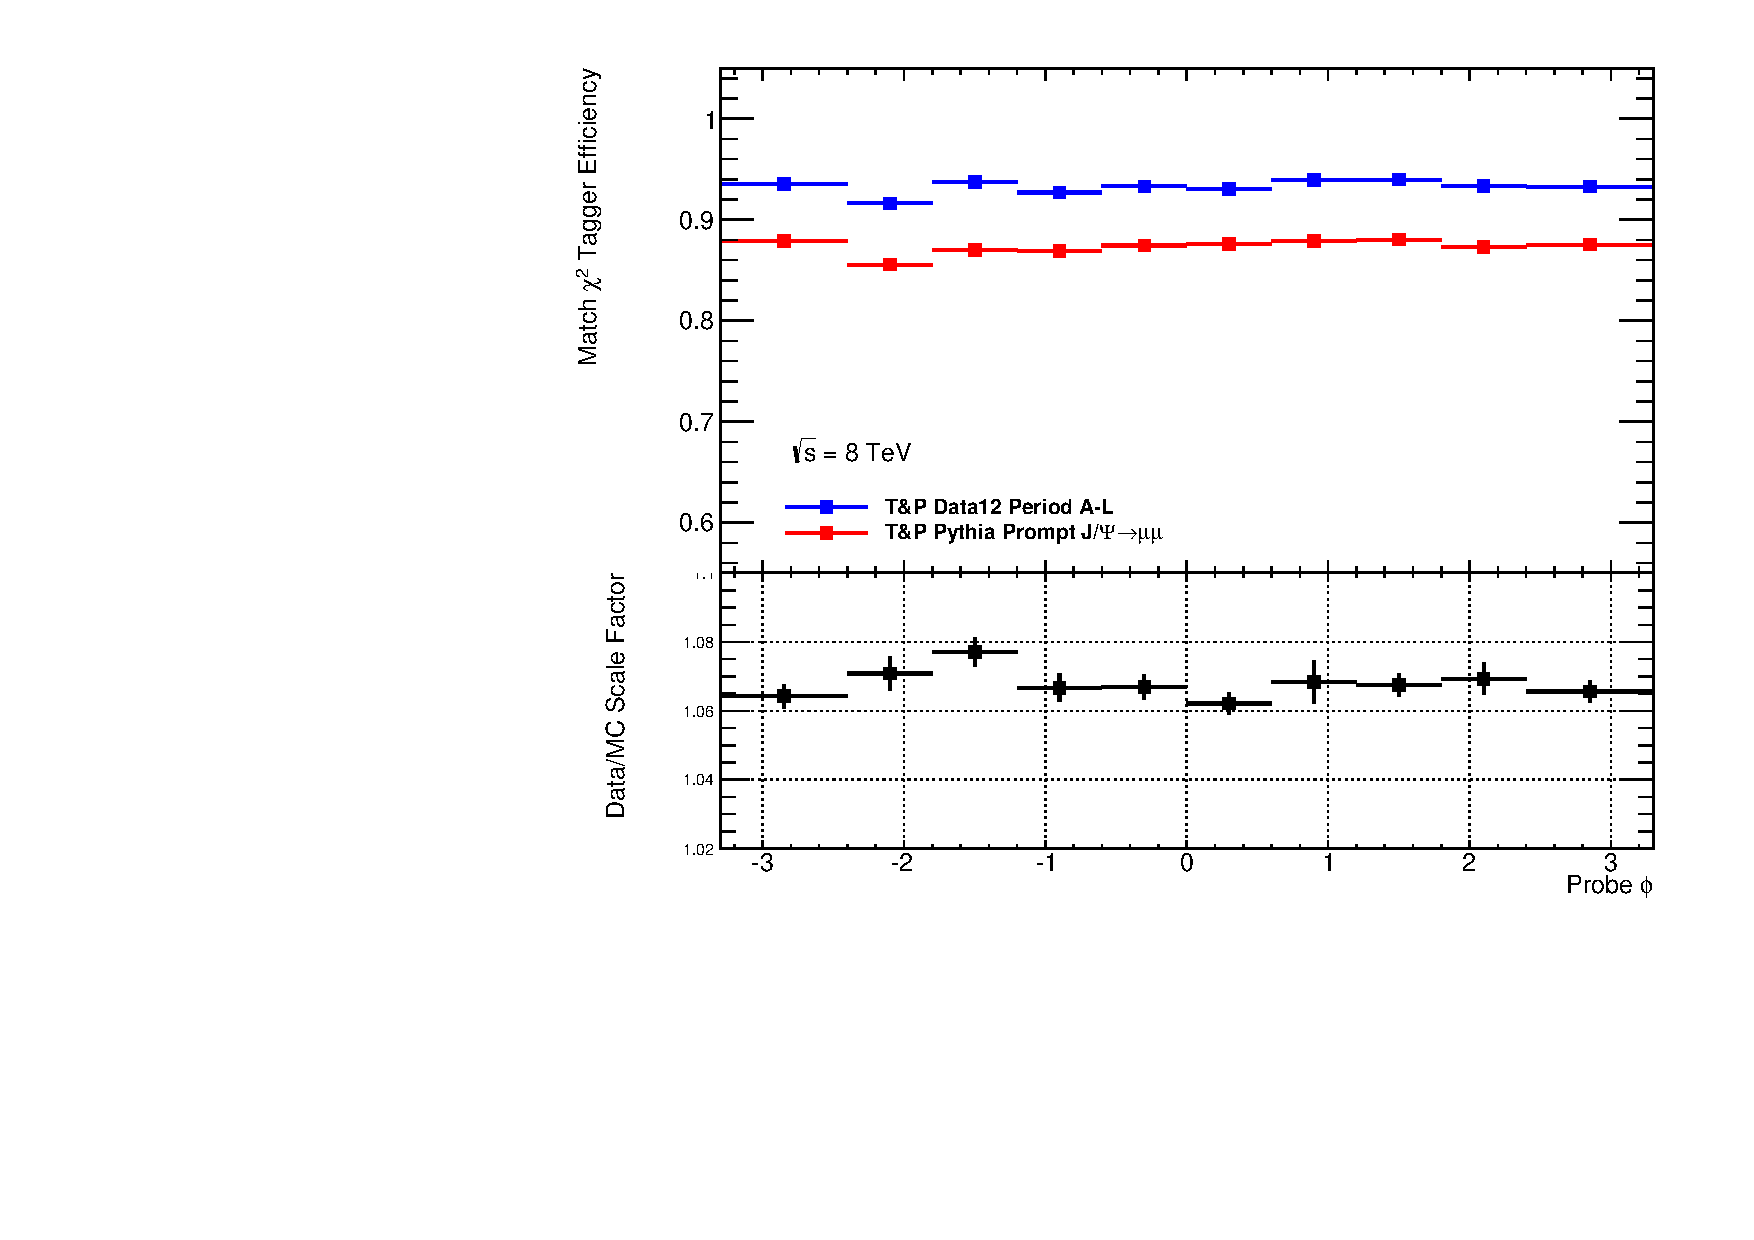
\includegraphics[width=\textwidth]{PartCalibration2012/Plots/SFPlots/phi_smt.pdf}
      \caption{\xsm\ efficiency and scale factor as a function of the azimuthal angle $\phi$ of the probe muon.}\label{fig:CalibrationPhi}
  \end{subfigure}

  \begin{subfigure}[b]{0.75\textwidth}
      \includegraphics[width=\textwidth]{PartCalibration2012/Plots/SFPlots/eta_smt.pdf}
      \caption{\xsm\ efficiency and scale factor as a function of the pseudorapidity $\eta$ of the probe muon.}\label{fig:CalibrationEta}
  \end{subfigure}
  \caption[Distribution of the \xsm\ efficiency as measured in data and MC, and the associated scale factor with respect to the azimuthal angle $\phi$ and the pseudorapidity $\eta$ of the muon probe.]{Distribution of the \xsm\ efficiency as measured in data and MC, and the associated scale factor with respect to the~\subref{fig:CalibrationPhi} azimuthal angle $\phi$ and~\subref{fig:CalibrationEta} the pseudorapidity $\eta$ of the muon probe.}\label{fig:CalibrationAngularResults}
\end{figure}

% SF vs PT
\begin{figure}[htbp]
  \centering
    \includegraphics[width=0.75\textwidth]{PartCalibration2012/Plots/SFPlots/pt_smt.pdf}
    \caption{Distribution of the \xsm\ efficiency as measured in data and MC, and the associated scale factor with respect to the transverse momentum of the muon probe.}\label{fig:CalibrationMomentumResults}
\end{figure}

The SMT scale factors and their total uncertainties are summarized in Table~\ref{tab:Calibration2012SF}. As an example of the typical uncertainties obtained, the SMT efficiencies measured for muon probes with \pt\ in the range \SIrange[range-units=single]{5}{6}{\GeV} in the positive barrel region are
%
\begin{align*} 
  \epsilon_{\textrm{Data}} &= \fulleff{94.15}{0.32}{0.02}{0.10} \\
  \epsilon_{\textrm{MC}}   &= \fulleff{89.01}{0.01}{0.01}{0.07}
\end{align*}

As expected, the background uncertainty dominates in collision data while in simulation it represents the smallest source of uncertainty. The width of the \jpsi\ peak increases for forward probes, overwhelming the background distribution delimited by the trigger ``shoulders''. This is reflected in increased fit parameter uncertainties and a larger background uncertainty.

% Crack Region
\begin{figure}[htbp]
  \centering
    \begin{subfigure}[b]{0.85\textwidth}
        \includegraphics[width=\textwidth]{PartCalibration2012/Plots/SFPlots/Crack_A_smt.pdf}
        \caption{Crack A Region.}\label{fig:CalibrationScaleFactorCrackA}
    \end{subfigure}
  
    \begin{subfigure}[b]{0.85\textwidth}
        \includegraphics[width=\textwidth]{PartCalibration2012/Plots/SFPlots/Crack_C_smt.pdf}
        \caption{Crack C Region.}\label{fig:CalibrationScaleFactorCrackC}
    \end{subfigure}
    \caption[\xsm\ efficiencies and scale factors in the crack region of the detector for side A and C.]{\xsm\ efficiencies and scale factors in the crack region of the detector for side \subref{fig:CalibrationScaleFactorCrackA} A and \subref{fig:CalibrationScaleFactorCrackC} C.}\label{fig:CalibrationScaleFactorCrack}
\end{figure}

% Barrel Region
\begin{figure}[htbp]
  \centering
    \begin{subfigure}[b]{0.85\textwidth}
        \includegraphics[width=\textwidth]{PartCalibration2012/Plots/SFPlots/Barrel_A_smt.pdf}
        \caption{Barrel A Region.}\label{fig:CalibrationScaleFactorBarrelA}
    \end{subfigure}
    
    \begin{subfigure}[b]{0.85\textwidth}
        \includegraphics[width=\textwidth]{PartCalibration2012/Plots/SFPlots/Barrel_C_smt.pdf}
        \caption{Barrel C Region.}\label{fig:CalibrationScaleFactorBarrelC}
    \end{subfigure}
    \caption[\xsm\ efficiencies and scale factors in the barrel region of the detector for side A and C.]{\xsm\ efficiencies and scale factors in the barrel region of the detector for side \subref{fig:CalibrationScaleFactorBarrelA} A and \subref{fig:CalibrationScaleFactorBarrelC} C.}\label{fig:CalibrationScaleFactorBarrel}
\end{figure}

% Transition Region
\begin{figure}[htbp]
  \centering
  \begin{subfigure}[b]{0.85\textwidth}
    \includegraphics[width=\textwidth]{PartCalibration2012/Plots/SFPlots/Transition_A_smt.pdf}
    \caption{Transition A Region.}\label{fig:CalibrationScaleFactorTransitionA}
  \end{subfigure}
  
  \begin{subfigure}[b]{0.85\textwidth}
    \includegraphics[width=\textwidth]{PartCalibration2012/Plots/SFPlots/Transition_C_smt.pdf}
    \caption{Transition C Region.}\label{fig:CalibrationScaleFactorTransitionC}
  \end{subfigure}
  \caption[\xsm\ efficiencies and scale factors in the transition region of the detector for side A and C.]{\xsm\ efficiencies and scale factors in the transition region of the detector for side \subref{fig:CalibrationScaleFactorTransitionA} A and \subref{fig:CalibrationScaleFactorTransitionC} C.}\label{fig:CalibrationScaleFactorTransition}
\end{figure}

% Endcap Region
\begin{figure}[htbp]
  \centering
  \begin{subfigure}[b]{0.85\textwidth}
    \includegraphics[width=\textwidth]{PartCalibration2012/Plots/SFPlots/Endcap_A_smt.pdf}
    \caption{End-cap A Region.}\label{fig:CalibrationScaleFactorEndcapA}
  \end{subfigure}
  
  \begin{subfigure}[b]{0.85\textwidth}
    \includegraphics[width=\textwidth]{PartCalibration2012/Plots/SFPlots/Endcap_C_smt.pdf}
    \caption{End-cap C Region.}\label{fig:CalibrationScaleFactorEndcapC}
  \end{subfigure}
  \caption[\xsm\ efficiencies and scale factors in the end-cap region of the detector for side A and C.]{\xsm\ efficiencies and scale factors in the end-cap region of the detector for side \subref{fig:CalibrationScaleFactorEndcapA} A and \subref{fig:CalibrationScaleFactorEndcapC} C.}\label{fig:CalibrationScaleFactorEndcap}
\end{figure}

% Forward Region
\begin{figure}[htbp]
  \centering
  \begin{subfigure}[b]{0.85\textwidth}
    \includegraphics[width=\textwidth]{PartCalibration2012/Plots/SFPlots/Forward_A_smt.pdf}
    \caption{Forward A Region.}\label{fig:CalibrationScaleFactorForwardA}
  \end{subfigure}
  
  \begin{subfigure}[b]{0.85\textwidth}
    \includegraphics[width=\textwidth]{PartCalibration2012/Plots/SFPlots/Forward_C_smt.pdf}
    \caption{Forward C Region.}\label{fig:CalibrationScaleFactorForwardC}
  \end{subfigure}
  \caption[\xsm\ efficiencies and scale factors in the forward region of the detector for side A and C.]{\xsm\ efficiencies and scale factors in the forward region of the detector for side \subref{fig:CalibrationScaleFactorForwardA} A and \subref{fig:CalibrationScaleFactorForwardC} C.}\label{fig:CalibrationScaleFactorForward}
\end{figure}

% Table of 2012 SF
\begin{table}[htbp]
  \centering
  \tabcolsep=0.11cm
  \ra{1.3}
  \begin{tabular}{@{}%
                    l%
                    *{5}{S[table-format=1.3(3)]}%
                  @{}}
  \toprule
  \pt\ range [\si{\GeV}]   & \multicolumn{5}{c}{Scale Factor in} \\
  \midrule
  \textbf{Side A}          & {Crack}   & {Barrel}  & {Transition} & {End-cap}  & {Forward} \\
  \tabin\numrange{4}{5}   & 1.051(14) & 1.053(1)  & 1.045(5)     & 1.059(2)  & 1.088(2)  \\
  \tabin\numrange{5}{6}   & 1.051(5)  & 1.058(1)  & 1.057(5)     & 1.062(10) & 1.106(3)  \\
  \tabin\numrange{6}{7}   & 1.068(6)  & 1.066(1)  & 1.069(4)     & 1.066(2)  & 1.132(3)  \\
  \tabin\numrange{7}{8}   & 1.061(6)  & 1.063(1)  & 1.065(4)     & 1.062(2)  & 1.142(3)  \\
  \tabin\numrange{8}{10}  & 1.061(16) & 1.063(1)  & 1.068(4)     & 1.063(2)  & 1.161(3)  \\
  \tabin\numrange{10}{12} & 1.057(24) & 1.071(6)  & 1.062(7)     & 1.060(15) & 1.171(6)  \\
  \tabin\numrange{12}{14} & 1.059(16) & 1.062(3)  & 1.070(10)    & 1.057(20) & 1.178(12) \\
  \tabin\numrange{14}{16} & 1.043(68) & 1.069(13) & 1.076(43)    & 1.069(6)  & 1.204(13) \\
  \tabin\numrange{16}{20} & 1.027(77) & 1.077(6)  & 1.112(19)    & 1.067(4)  & 1.208(9)  \\
  \midrule
  \textbf{Side C}          & {Crack}   & {Barrel}  & {Transition} & {End-cap}  & {Forward} \\ 
  \tabin\numrange{4}{5}   & 1.044(14) & 1.055(1)  & 1.053(4)     & 1.056(2)  & 1.064(5)  \\
  \tabin\numrange{5}{6}   & 1.069(5)  & 1.057(1)  & 1.050(15)    & 1.061(8)  & 1.083(3)  \\
  \tabin\numrange{6}{7}   & 1.080(5)  & 1.068(4)  & 1.065(4)     & 1.065(2)  & 1.095(3)  \\
  \tabin\numrange{7}{8}   & 1.064(17) & 1.068(5)  & 1.061(5)     & 1.066(2)  & 1.100(4)  \\
  \tabin\numrange{8}{10}  & 1.070(7)  & 1.067(4)  & 1.054(5)     & 1.061(2)  & 1.101(3)  \\
  \tabin\numrange{10}{12} & 1.089(10) & 1.073(3)  & 1.083(22)    & 1.062(3)  & 1.107(6)  \\
  \tabin\numrange{12}{14} & 1.095(15) & 1.069(9)  & 1.063(28)    & 1.049(5)  & 1.114(8)  \\
  \tabin\numrange{14}{16} & 1.059(32) & 1.076(6)  & 1.085(14)    & 1.061(6)  & 1.107(13) \\
  \tabin\numrange{16}{20} & 1.109(32) & 1.088(3)  & 1.096(21)    & 1.050(4)  & 1.120(9)  \\
  \bottomrule
  \end{tabular}
  \caption[Data/MC Scale Factors for 2012 Data in all five regions of the detector as a function of \pt.]{Data/MC Scale Factors for 2012 Data in all five regions of the detector as a function of \pt. The uncertainties include systematic and statistical components as described in Section~\ref{sec:CalibrationUncertainty}.}\label{tab:Calibration2012SF}
\end{table}

\subsubsection{Isolation dependence}\label{sec:CalibrationEfficienciesIsolation}

The muons from \jpsi\ used in this calibration are produced in isolation, meaning there is very little energetic activity surrounding them in the detector. In contrast, muons from semileptonic decay of $b$-quarks in \ttbar\ events are produced amongst the tracks associated with the $b$-jet.

\begin{figure}[htbp]
  \centering
  \includegraphics[width=0.75\textwidth]{PartCalibration2012/Plots/Kinematics/h_etcone20_smt_mu.pdf}
  \caption{Distribution of the cluster-based isolation within a cone of size $\DeltaR=0.2$ for muons coming from $W$ decays (solid) and from semileptonic $b$-decays (dashed) in \ttbar\ events.}\label{fig:CalibrationEtcone20Dist}
\end{figure}

For the results of the calibration on \jpsi\ to be applicable, the performance of the \xsm\ tagger must not affected by the isolation of the muon. In this calibration, the nine isolation variables defined in Section~\ref{sec:DetectorElReco} are considered.

The isolated nature of muons in \jpsi\ events limits the number of muons available at higher pt/et/nucone values. This is more significant in simulation compared to the collision data which contains non-isolated muons. There appears to be no dependence on any of the isolation variables examined (Figures~\ref{fig:CalibrationIsoEtcone},~\ref{fig:CalibrationIsoPtcone} and~\ref{fig:CalibrationIsoNucone}).

% etcone
\begin{figure}[htbp]
  \centering
    \begin{subfigure}[b]{0.54\textwidth}
      \includegraphics[width=\textwidth]{PartCalibration2012/Plots/SFPlots/etcone20_smt.pdf}
      \caption{$\sum \Et$ in cone $\Delta R=0.2$}\label{fig:CalibrationIsoEtcone20}
    \end{subfigure}
    
    \begin{subfigure}[b]{0.54\textwidth}
      \includegraphics[width=\textwidth]{PartCalibration2012/Plots/SFPlots/etcone30_smt.pdf}
      \caption{$\sum \Et$ in cone $\Delta R=0.3$}\label{fig:CalibrationIsoEtcone30}
    \end{subfigure}

    \begin{subfigure}[b]{0.54\textwidth}
      \includegraphics[width=\textwidth]{PartCalibration2012/Plots/SFPlots/etcone40_smt.pdf}
      \caption{$\sum \Et$ in cone $\Delta R=0.4$}\label{fig:CalibrationIsoEtcone40}
    \end{subfigure}
  \caption{\xsd\ efficiencies and scale factor with respect to $\sum \Et$ for a muon probe that passes the SMT requirements.}\label{fig:CalibrationIsoEtcone}
\end{figure}

% ptcone
\begin{figure}[htbp]
  \centering
    \begin{subfigure}[b]{0.54\textwidth}
      \includegraphics[width=\textwidth]{PartCalibration2012/Plots/SFPlots/ptcone20_smt.pdf}
      \caption{$\sum \pt$ in cone $\Delta R=0.2$}\label{fig:CalibrationIsoPtcone20}
    \end{subfigure}
    
    \begin{subfigure}[b]{0.54\textwidth}
      \includegraphics[width=\textwidth]{PartCalibration2012/Plots/SFPlots/ptcone30_smt.pdf}
      \caption{$\sum \pt$ in cone $\Delta R=0.3$}\label{fig:CalibrationIsoPtcone30}
    \end{subfigure}
    
    \begin{subfigure}[b]{0.54\textwidth}
      \includegraphics[width=\textwidth]{PartCalibration2012/Plots/SFPlots/ptcone40_smt.pdf}
      \caption{$\sum \pt$ in cone $\Delta R=0.4$}\label{fig:CalibrationIsoPtcone40}
    \end{subfigure}
  \caption{\xsd\ efficiencies and scale factor with respect to $\sum \pt$ for a muon probe that passes the SMT requirements.}\label{fig:CalibrationIsoPtcone}
\end{figure}

% nucone
\begin{figure}[htbp]
  \centering
    \begin{subfigure}[b]{0.54\textwidth}
      \includegraphics[width=\textwidth]{PartCalibration2012/Plots/SFPlots/nucone20_smt.pdf}  
      \caption{$N_{\textrm{trk}}$ in cone $\Delta R=0.2$}\label{fig:CalibrationIsoNucone20}
    \end{subfigure}
    
    \begin{subfigure}[b]{0.54\textwidth}
      \includegraphics[width=\textwidth]{PartCalibration2012/Plots/SFPlots/nucone30_smt.pdf}
      \caption{$N_{\textrm{trk}}$ in cone $\Delta R=0.3$}\label{fig:CalibrationIsoNucone30}
    \end{subfigure}
    
    \begin{subfigure}[b]{0.54\textwidth}
      \includegraphics[width=\textwidth]{PartCalibration2012/Plots/SFPlots/nucone40_smt.pdf}
      \caption{$N_{\textrm{trk}}$ in cone $\Delta R=0.4$}\label{fig:CalibrationIsoNucone40}
    \end{subfigure}
  \caption{\xsd\ efficiencies and scale factor with to $N_{\textrm{tracks}}$ for a muon probe that passes the SMT requirements.}\label{fig:CalibrationIsoNucone}
\end{figure}

\subsubsection*{Dependence on $d_{0}$}

The dependence on the impact parameter $d_{0}$ was examined and no direct dependence is observed. The scale factor shows no structure with respect to $d_{0}$ when binned in \pt\ (Figure~\ref{fig:CalibrationD0Results}). Since the scale factors are binned in $\eta$ and \pt, the correlation between $d_{0}$ and \pt\ is taken into account.

\begin{figure}[htbp]
  \centering
  \sisetup{range-units=single}
  \begin{subfigure}[b]{0.52\textwidth}
    \includegraphics[width=\textwidth]{PartCalibration2012/Plots/SFPlots/ptCourse_4_6__smt.pdf}
    \caption{$\SI{4}{\GeV}<\pt<\SI{6}{\GeV}$}\label{fig:CalibrationD04to6}
  \end{subfigure}
  
  \begin{subfigure}[b]{0.52\textwidth}
    \includegraphics[width=\textwidth]{PartCalibration2012/Plots/SFPlots/ptCourse_6_8__smt.pdf}
    \caption{$\SI{6}{\GeV}<\pt<\SI{8}{\GeV}$}\label{fig:CalibrationD06to8}
  \end{subfigure}

  \begin{subfigure}[b]{0.52\textwidth}
    \includegraphics[width=\textwidth]{PartCalibration2012/Plots/SFPlots/ptCourse_8_10__smt.pdf}
    \caption{$\SI{8}{\GeV}<\pt<\SI{10}{\GeV}$}\label{fig:CalibrationD08to10}
  \end{subfigure}
  \caption[Distribution of the \xsm\ efficiencies and scale factor with respect to impact parameter $d_{0}$ for muon probes with \pt\ in the ranges \SIrange{4}{6}{\GeV}, \SIrange{6}{8}{\GeV} and \SIrange{8}{10}{\GeV}.]{Distribution of the \xsm\ efficiencies and scale factor with respect to impact parameter $d_{0}$ for muon probes with \pt\ in the ranges \subref{fig:CalibrationD04to6} \SIrange{4}{6}{\GeV}, \subref{fig:CalibrationD06to8} \SIrange{6}{8}{\GeV} and \subref{fig:CalibrationD08to10} \SIrange{8}{10}{\GeV}. The measurement was carried out only on Period B of 2012 ATLAS collision data.}\label{fig:CalibrationD0Results}
\end{figure}

\section{Scale factor discrepancy}

A discrepancy between the 2011 and 2012 scale factors is observed. The SFs in the 2011 analysis do not deviate substantially from unity, while the 2012 SFs deviate as much as \SI{15}{\percent}. The efficiency measured in the 2012 collision data appears to be consistent with the 2011 result, however in simulation the efficiency is measured to be lower. The difference in SF appears to come from a mismodelling of the \xsd\ variable. 

A number of factors can contribute to such a mismodelling including inaccurate description of the alignment of detector components, and the description of the material used in the detector. Both of these can result in mismodelling of the kinematic variables that make up the \xsd\ variable.

In order to find the source of the discrepancy the components of the \xsd\ variable were examined. The \emph{pull} of a kinematic variable is defined here as
%
\begin{equation}
  X_{\textrm{pull}} = \frac{X^{\textrm{ID}} - X^\textrm{ME}}{\sqrt{\sigma^{2}_{X^{\textrm{ID}}} + \sigma^{2}_{X^{\textrm{ME}}}}}
  \label{eq:CalibrationPull}
\end{equation}
%
where $X$ is any of the five kinematic components of \xsm, and $\sigma$ is the uncertainty on that variable. The pulls are shown in terms of the azimuthal angle, the polar angle, the longitudinal and transverse impact parameters and the charge over momentum ($q\ p$) of the muon probe in in Figure~\ref{fig:CalibrationPull}. The transverse momentum is related to the $q/p$ by $\pt=|1/(q/p)|\sin(\theta)$ and the pseudorapidity is defined in terms of the angle $\theta$ in Section~\ref{ch:Detector}. The momentum appears to be well modelled in MC as can be seen from the pull distribution. The $d_0$ and $\theta$ distributions do not appear well modelled in MC\@. By construction the two variables are strongly correlated~\cite{Calibration:TrackingSlides}, so its not unexpected to observe a discrepancy simultaneously in both of these arguments. Such a discrepancy could be caused by a mismodelling of the alignment of the detector components.

% Pull Plots
\begin{figure}[htbp]
  \centering
    \begin{subfigure}[b]{0.49\textwidth}
      \includegraphics[width=\textwidth]{PartCalibration2012/Plots/DiscrepancyStudy/Pull/h_pull_theta_Nominal.eps}
      \caption{}\label{fig:CalibrationPullEta}
    \end{subfigure}
    \hfill
    \begin{subfigure}[b]{0.49\textwidth}
      \includegraphics[width=\textwidth]{PartCalibration2012/Plots/DiscrepancyStudy/Pull/h_pull_phi_Nominal.eps}
      \caption{}\label{fig:CalibrationPullPhi}
    \end{subfigure}

    \begin{subfigure}[b]{0.49\textwidth}
      \includegraphics[width=\textwidth]{PartCalibration2012/Plots/DiscrepancyStudy/Pull/h_pull_d0_Nominal.eps}
      \caption{}\label{fig:CalibrationPullD0}
    \end{subfigure}
    \hfill
    \begin{subfigure}[b]{0.49\textwidth}
      \includegraphics[width=\textwidth]{PartCalibration2012/Plots/DiscrepancyStudy/Pull/h_pull_z0_Nominal.eps}
      \caption{}\label{fig:CalibrationPullZ0}
    \end{subfigure}

    \begin{subfigure}[b]{0.49\textwidth}
      \includegraphics[width=\textwidth]{PartCalibration2012/Plots/DiscrepancyStudy/Pull/h_pull_qoverp_Nominal.eps}
      \caption{}\label{fig:CalibrationPullPt}
    \end{subfigure}
    \caption[Distribution of the pull of components of \xsd\ as measured in the ID for muon probes in the barrel region for collision data (squares) and prompt \jpsi\ simulation (dotted).]{Distribution of the pull (see~\ref{eq:CalibrationPull}) of components of \xsd\ as measured in the ID for muon probes in the barrel region for collision data (squares) and prompt \jpsi\ simulation (dotted). Shown are~\subref{fig:CalibrationPullEta} $\theta$,~\subref{fig:CalibrationPullPhi} $\phi$,~\subref{fig:CalibrationPullD0} $d_{0}$,~\subref{fig:CalibrationPullZ0} $z_{0}$ and~\subref{fig:CalibrationPullPt} $q$/$p$. These distributions are based on smaller samples and are normalized to unit area.}\label{fig:CalibrationPull}
\end{figure}

A study to test the effects of different alignment profiles was carried out. Several samples with different alignment profiles were compared to a small sample of \SI{8}{\TeV} collision data from a single run. These include the nominal prompt \jpsi\ sample used in this calibration, the \jpsi\ sample used for the 2011 calibration, a \ZMu\ sample where the detector is perfectly aligned, a 2011 \ZMu\ sample with an updated detector geometry description, and a \ZMu\ sample with the nominal smeared alignment. The smeared alignment is produced by distorting the ideal alignment sample within the current measured alignment uncertainties. This procedure is not designed to perfectly represent the details in the misalignment of the ATLAS detector, but rather simulates a detector which is as well aligned as the real detector. These two profiles are compared in small samples of \ZMu\ events.

A sample of well reconstructed muons is selected by matching STACO CB muons to truth muons from $Z$ or \jpsi. The \xsd\ distribution of these muons is then compared for muons with \pt\ between \num{4} and \SI{25}{\GeV}.

As expected, the alignment profile does have an effect on the \xsd\ distribution, particularly in the lower end (Figure~\ref{fig:CalibrationAlignment}). However, this effect is not sufficiently large to account, on its own, for the discrepancy between simulation and data in all bins. A pseudo-efficiency of the \xsm\ selection is obtained by taking the area under the curve below \num{3.2} and dividing it to the total area. The results are summarized in Table~\ref{tab:CalibrationProfileEffs}. The overall difference between the 2011 and 2012 \jpsi\ samples is approximately \SI{5}{\percent}, not sufficient to cover the discrepancy between data and MC\@.

\begin{table}[htbp]
  \centering
  \begin{tabular}{@{}lS[table-format=2.2(1)]@{}}
    \toprule
    Sample                      & {Pseudo-efficiency [\si{\percent}]} \\
    \midrule
    \textbf{Data } $\boldsymbol{\cmsE}$ & 94.35(2) \\
    $\boldsymbol{\JMu}$ \\
    \tabin Nominal 2011         & 95.22(2) \\
    \tabin Nominal 2012         & 90.59(2) \\
    $\boldsymbol{\ZMu}$ \\
    \tabin Nominal 2012         & 92.44(3) \\
    \tabin Ideal alignment 2012 & 91.37(3) \\
    \tabin New geometry 2011    & 91.43(3) \\
    \bottomrule
  \end{tabular}
  \caption{Summary of \xsm\ tagger efficiencies as measured in all tested samples.}\label{tab:CalibrationProfileEffs}
\end{table}

\begin{figure}[htbp]
  \centering
    \includegraphics[width=0.85\textwidth]{PartCalibration2012/Plots/FixingMomImba/h\string_muon\string_matchchi2\string_ndof.eps}
    \caption{Distribution of \xsd\ of STACO CB muons from collision data (circle), a nominal 2012 \ZMu\ sample (solid), a 2012 \ZMu\ sample with ideal detector alignment (dashed), a 2011 \ZMu\ sample with updated detector description (dashed-double dot), \JMu\ with nominal alignment at \cmsE\ (solid) and \JMu\ with smeared at \cmsS\ as used in the 2011 analysis (dotted). Distributions are normalized to unit area.}\label{fig:CalibrationAlignment}
\end{figure}

\subsection{Future developments}

As can be seen from Figure~\ref{fig:CalibrationPullPt}, the momentum appears to be well modelled in both data and simulation. As a result, an alternative variable known as the momentum imbalance is currently being studied. The momentum imbalance is defined as
%
\begin{equation}
  \textrm{Mom. Imb.} = \frac{p^{\textrm{ID}} - p^{\textrm{ME}}}{p^{\textrm{ID}}}
\end{equation}
%
where $p^{\textrm{ID}}$ is the momentum of the muon track as measured in the ID and $p^{\textrm{ME}}$ is measured in the MS extrapolated back to the primary vertex. This extrapolation takes into account the loss of momentum that occurs when the muon traverses through the detector material.

The momentum imbalance distribution for the aforementioned samples is shown in Figure~\ref{fig:CalibrationMomImba}. Measurements of the efficiency using momentum imbalance have been carried out, and the collision data results appear to be well-modelled in simulation. The selection using momentum imbalance requires $\textrm{Mom. Imb.}<\num{0.1}$ as background sources tend to peak above this threshold. From full studies currently being carried out, the momentum imbalance at this operating point exhibits similar performance to the \xsm\ version of the tagger.

The pseudo-efficiency for this selection as measured in the aforementioned samples are shown in Table~\ref{tab:CalibrationMomImbaProfileEffs}. These appear to be less affected by the transition from 2011 reconstruction and 2012 reconstruction techniques. In addition, changes in the detector alignment and geometry description affect the pseudo-efficiency substantially less than the \xsd\ selection. 

\begin{table}[htbp]
  \centering
    \begin{tabular}{@{}lS[table-format=2.2(1)]@{}}
      \toprule
      Sample                   & {Pseudo-efficiency [\si{\percent}]} \\
      \midrule
      $\boldsymbol{\JMu}$ \\
      \tabin Nominal 2011           & 92.81(2) \\
      \tabin Nominal 2012           & 93.57(2) \\
      $\boldsymbol{\ZMu}$ \\
      \tabin New geometry 2011      & 94.20(3) \\
      \tabin Nominal 2012           & 94.19(3) \\
      \tabin Ideal alignment 2012   & 94.46(2) \\
      \bottomrule
    \end{tabular}
    \caption{Summary of momentum imbalance efficiencies as measured in all tested samples.}\label{tab:CalibrationMomImbaProfileEffs}
\end{table}

\begin{figure}[htbp]
  \centering
    \includegraphics[width=0.85\textwidth]{PartCalibration2012/Plots/FixingMomImba/h_muon_momImba.eps}
    \caption{Distribution of momentum imbalance of STACO CB muons from a nominal 2012 \ZMu\ sample (solid), a 2012 \ZMu\ sample with ideal detector alignment (dashed), a 2011 \ZMu\ sample with updated detector description (dashed-double dot), \JMu\ with nominal alignment at \cmsE\ (solid) and \JMu\ with smeared at \cmsS\ as used in the 2011 analysis (dotted). Distributions are normalized to unit area.}\label{fig:CalibrationMomImba}
\end{figure}

Following a comparison of the reconstruction efficiencies with those obtained by members of the MCP group, the pairing selection has been loosened to allow for multiple probes per tag. It is possible for the correct probe to be further away from the tag in $z_0$ than other spurious tracks. By forcing the selection of the closest ID track in $z_0$, the sample of probes is contaminated with non-muons resulting in a lower than expected reconstruction efficiency. This increases the statistics available for invariant mass fitting and more importantly, has increased the reconstruction efficiency across the $\eta$-\pt\ phase space.

% !TEX root = ../Thesis.tex
\newcommand{\Wplus}{\ensuremath{W^{+}}}
\newcommand{\Wminus}{\ensuremath{W^{-}}}
\newcommand{\yield}[3]{\ensuremath{#1\,^{+\,\num{#2}}_{-\,\num{#3}}}}
\newcommand{\cellc}[1]{\multicolumn{1}{c}{#1}}
\newcommand{\wpretag}{W_{\textrm{pretag}}}
\newcommand{\wtag}{W_{\textrm{tag}}}
\newcommand{\rtag}{R_{\textrm{tag}}}
\newcommand{\asymUncA}[3]{\ensuremath{^{\SI[explicit-sign=+]{+#1}{#3}}_{\SI{-#2}{#3}}}}
\newcommand{\asymUnc}[4]{\num{#1}\;^{+\;#2}_{-\;#3}\;#4}
\newcommand{\ejets}{$e$+jets}
\newcommand{\mujets}{$\mu$+jets}

\chapter[Measurement of the \texorpdfstring{\ttbar}{top-antitop} cross section]{Measurement of the $\bm{\ttbar}$ cross section in the $\bm{\ell}$+jets channel using SMT}\label{ch:CrossSection}

This section describes a \ttbar\ cross section measurement carried out by the joint RHUL and QMUL group.

Presented here is a measurement of the top quark pair production cross section at \cmsS\ in the lepton plus jets channel, with at least one of the $b$-quarks in the event decaying semileptonically producing a soft muon. The presence of such a jet is determined by the use of the \xsm-based SMT tagger described in Section~\ref{sec:DetectorSLT}.

\section{Collision data and simulated samples}\label{sec:CrossSectionSamplesMC}

This measurement is based on collision data recorded by ATLAS in 2011 at the LHC running with \cmsS. After applying quality cuts based on the beam and detector conditions, the dataset contains an integrated luminosity of \SI{4.66(8)}{\per\femto\barn}. Several simulated samples are used in this analysis, including the signal process and all backgrounds excluding the multijet background source. The \ttbar\ signal sample was simulated with MC@NLO v4.01~\cite{CrossSection:MCNLOFirst,CrossSection:MCNLOSecond} interfaced to HERWIG~\cite{Herwig} for parton showering and hadronization, and JIMMY~\cite{CrossSection:Jimmy} for underlying event simulation. The $W/Z$+jets samples were generated using ALPGEN~\cite{CrossSection:ALPGEN} interfaced into HERWIG+JIMMY. The single top samples were generated using MC@NLO interfaced to HERWIG+JIMMY for the $s$ and $Wt$ channels, and AcerMC~\cite{CrossSection:ACERMC} interfaced to PYTHIA~\cite{Pythia} for the $t$ channel. Finally, the diboson samples ($WW/WZ/ZZ$) were generated using HERWIG alone. 

This analysis is based on the tagging of muons from semileptonic decays of $b$-quarks. In order to obtain accurate event yields it is important that the simulation correctly models the inclusive production rate of soft muons, and the individual BR for all production chains (Table~\ref{tab:DetectorSLTBR}). To this end, each event with a soft muon is re-weighted such that the BRs conform with the latest measured values as quoted in Ref.~\cite{Theory:PDGBooklet}. The reference BR and the values used by HERWIG and PYTHIA are shown in Table~\ref{tab:CrossSectionBRbTomu}.

\begin{table}
  \centering
  \begin{tabular}{@{}
                    l%
                    S[table-format=2.2(2)]%
                    S[table-format=2.2(2)]%
                    @{~(}
                    S[table-format=1.2(2),tight-spacing=true,table-space-text-pre=(,table-space-text-post=)]%
                    @{)\;}
                    S[table-format=2.2(2)]%
                    @{~(}
                    S[table-format=1.2(2),tight-spacing=true,table-space-text-pre=(,table-space-text-post=)]%
                  @{)}}
    \toprule
    Source & \multicolumn{5}{c}{Branching Ratio [\si{\percent}] (Ratio to PDG)} \\
    \cmidrule{2-6}
                                    & {PDG} & \multicolumn{2}{c}{HERWIG} & \multicolumn{2}{c}{PYTHIA} \\
    \midrule
    $b\rightarrow \mu$                         & 10.95(29) & 9.57(3) & 1.14(3) & 10.01(3) & 1.09(3)   \\
    $b\rightarrow \tau \rightarrow \mu$        & 0.42(4)   & 0.70(2) & 0.60(6) & 0.67(1)  & 0.62(6)   \\
    $b\rightarrow c \rightarrow \mu^{+}$       & 8.02(19)  & 8.24(3) & 0.97(2) & 8.89(3)  & 0.90(2)   \\
    $b\rightarrow \bar{c} \rightarrow \mu^{-}$ & 1.60(50)  & 2.51(2) & 0.64(20) & 2.66(2)  & 0.60(19) \\
    \bottomrule
  \end{tabular}
  \caption[List of the $b\rightarrow\mu$ branching ratios used in the HERWIG and PYTHIA generators compared to the reference PDG values.]{List of the $b\rightarrow\mu$ branching ratios used in the HERWIG and PYTHIA generators compared to the reference PDG values~\cite{Theory:PDGBooklet}.}\label{tab:CrossSectionBRbTomu}
\end{table}

\section{Object identification and event selection}\label{sec:CrossSectionEventSelection}

The selection criteria used in this analysis are based on the nominal \cmsS\ selections recommended by the ATLAS top group. Some alterations have been implemented to adapt to the usage of the \xsm\ tagger instead of the standard MV1 method for $b$-jet tagging. Collision and simulation events are required to have fired an inclusive single electron or muon trigger with offline-reconstructed candidates with $\pt>\SI{25}{\GeV}$ for electrons and $\pt>\SI{20}{\GeV}$ for muons. Electrons are required to have $|\eta|<\num{2.47}$ and not lie within the transition between the barrel and end-cap calorimeters ($\num{1.37}<|\eta|<\num{1.52}$). They must satisfy the \emph{tight} identification criteria as described in Appendix~\ref{app:DetectorElectronID}. Electrons are required to be isolated using cuts on calorimeter isolation (\etcone{20}) and momentum isolation (\ptcone{30}) as defined in Section~\ref{sec:CalibrationEfficienciesIsolation}. The cut values for both are defined so as to maintain an efficiency of \SI{90}{\percent}. The isolation requirements are designed to reduce the amount of multijet background where reconstructed electrons are not produced in isolation.

Muon candidates are reconstructed using the MUID combined algorithm (see Section~\ref{sec:MUID}), and must lie within the coverage of ID ($|\eta|<2.5$). The combined track is obtained by fitting hits in the ID and MS\@. The muon is required to be isolated in both tracking and calorimeter isolation with $\etcone{20}<\SI{4}{\GeV}$ and $\ptcone{30}<\SI{2.5}{\GeV}$, and to be well separated from the jet by at least $\DeltaR>0.4$. Events must contain exactly one selected muon or one selected electron.

Jets are reconstructed using the anti-$k_{t}$ algorithm with a distance parameter $R=0.4$. Topo-clusters at the EM scale are used as inputs to the algorithm and JES corrections are applied to the resulting jets. They are also required to have a $\pt>\SI{25}{\GeV}$ and $|\eta|<2.5$. The \emph{jet vertex fraction} (JVF) defined as:

\begin{equation}
  \textrm{JVF} = \frac{\sum \pt \textrm{ of jet tracks from PV}}{\sum \pt \textrm{ of all jet tracks}}
\end{equation}
%
has to be larger than \num{0.75}. The JVF cut is implemented to remove jets from minimum bias interactions.

Finally, jets within $\DeltaR<0.2$ of an electron are rejected.

In the \ejets\ analysis, a large amount of missing transverse energy is required ($>\SI{30}{\GeV}$) to account for the escaping neutrino. The transverse mass of the $W$ boson \mtw\ is reconstructed from the signal lepton and the missing transverse energy:

\begin{equation}
  \mtw=\sqrt{2\pt^{\ell}\pt^{\nu}[1-\cos{\phi^{\ell}-\phi^{\nu}}]}
\end{equation}
%
where \met\ is associated with the neutrino to calculate $\pt^{\nu}$ and $\phi^{\nu}$.

In the electron channel the measured \mtw\ must be larger than \SI{30}{\GeV}. The \met\ requirement in the \mujets\ channel is looser ($\met>\SI{20}{\GeV}$) and a triangular cut $\met+\mtw>\SI{60}{\GeV}$ is applied.

For both channels, a minimum of three selected jets is required. Given the final-state signature, it is reasonable to request four or more jets in the event. It was found that the three jets inclusive selection yielded a lower statistical uncertainty, and more importantly a smaller event generator systematic uncertainty. These uncertainties are described in more detail in Section~\ref{sec:systematics_uncertainties}.

All events which pass these selections are labelled as ``pretag'' events. Those events which contain at least one jet tagged by the SMT algorithm are labelled as ``tagged'' events. In the \mujets\ channel, requirements are placed on the invariant mass of the soft muon and the signal muon $m_{\mu\mu}$ to remove contributions from dimuon $\Upsilon$ ($\SI{8}{\GeV}\leq m_{\mu\mu} \leq\SI{11}{\GeV}$) and $Z$ ($\SI{80}{\GeV}\leq m_{\mu\mu}\leq\SI{100}{\GeV}$) decays. Finally, the signal muon must be a different object than the soft muon ($\DeltaR>0.01$).

The efficiency of the full selection as measured on the \ttbar\ signal sample is \SI{1.42}{\percent} in the \ejets\ channel and \SI{2.15}{\percent} in the \mujets\ channel. These efficiencies include both lepton plus jets and dilepton events with at least three jets and at least one jet tagged by the SMT algorithm. Acceptance to fully hadronic events is negligible.

\section{Background estimation}\label{sec:CrossSectionBacgkround}

Lepton plus jets \ttbar\ events have a varied final state signature that includes a lepton, multiple jets including $b$-jets and missing energy. As a result \ttbar\ analyses must take into account several sources of background: diboson, \W+jets, \Z+jets, single-top and multijet.

\W+jets events (e.g. Figure~\ref{fig:WbbJets}) enter the signal region due to the presence of a real lepton, missing transverse energy, and one or two real $b$-jets or mistagged LF jets. Gluon emissions can also occur resulting in additional jets. The \W+jets background is estimated using data-driven methods.

$Z$+jets events (e.g. Figure~\ref{fig:ZbbJets}) can pass the selection if one of the two leptons is not identified. This can happen if, for example, the lepton enters the crack region. This results in an overall imbalance of momentum interpreted as missing energy. The $Z$ boson can be created in association with a gluon which results in real $b$-jets or mistagged LF jets. This source of background, along with single-top and diboson, is estimated from MC simulation.

Diboson production (e.g. Figure~\ref{fig:WW}) such as $WW$, $ZZ$ or $WZ$ enters the signal region due to the presence of real leptons, missing energy (from real or missed leptons), and HF or mistagged LF jets.

\begin{figure}[htbp]
  \centering
    \begin{minipage}[][][t]{.45\textwidth}
      \centering
        % !TEX root = ../../../Thesis.tex
\begin{fmffile}{WJetsEx}
\fmfframe(5,17)(20,17) {
\begin{fmfgraph*}(85,80)
\fmfleft{qPrime,qBar}
\fmfright{b,bbar,lep,nu}
\fmf{fermion,tension=0.5}{qPrime,v1}
\fmf{gluon,label=$g$}{v1,v2}
\fmf{fermion,tension=0.5}{v3,qBar}
\fmf{fermion,tension=0.25}{v1,v3}
\fmf{boson,label=$W$}{v4,v3}
\fmf{fermion,tension=0.5}{bbar,v2,b}
\fmf{fermion,tension=0.5}{nu,v4,lep}
\fmflabel{$q'$}{qPrime} \fmflabel{$\bar{q}$}{qBar}
\fmflabel{$\ell$}{lep} \fmflabel{$\nu$}{nu}
\fmflabel{$\bar{b}$}{bbar} \fmflabel{$b$}{b}
\end{fmfgraph*}
}
\end{fmffile}
        \subcaption{$W\bar{b}b$+jets production.}\label{fig:WbbJets}
    \end{minipage}
    \,
    \begin{minipage}[][][t]{.45\textwidth}
      \centering
        % !TEX root = ../../../Thesis.tex
\begin{fmffile}{ZJetsEx}
\fmfframe(5,17)(20,17) {
\begin{fmfgraph*}(85,80)
\fmfleft{q,qBar}
\fmfright{b,bbar,lep,lep2}
\fmf{fermion,tension=0.5}{q,v1}
\fmf{gluon,label=$g$}{v1,v2}
\fmf{fermion,tension=0.5}{v3,qBar}
\fmf{fermion,tension=0.25}{v1,v3}
\fmf{boson,label=$Z$}{v4,v3}
\fmf{fermion,tension=0.5}{bbar,v2,b}
\fmf{fermion,tension=0.5}{lep2,v4,lep}
\fmflabel{$q$}{q} \fmflabel{$\bar{q}$}{qBar}
\fmflabel{$\ell$}{lep} \fmflabel{$(\ell)$}{lep2}
\fmflabel{$\bar{b}$}{bbar} \fmflabel{$b$}{b}
\end{fmfgraph*}
}
\end{fmffile}
        \subcaption{$Z\bar{b}b$+jets production.}\label{fig:ZbbJets}
    \end{minipage}
    
    \begin{minipage}[][][t]{.45\textwidth}
      \centering
        % !TEX root = ../../../Thesis.tex
\begin{fmffile}{DibosonEx}
\fmfframe(5,17)(20,17) {
\begin{fmfgraph*}(85,80)
\fmfleft{q,qBar}
\fmfright{qOut,qBarOut,lep,nu}
\fmf{fermion,tension=0.5}{q,v1}
\fmf{boson,label=$W$}{v1,v2}
\fmf{fermion,tension=0.5}{v3,qBar}
\fmf{fermion,tension=0.25}{v1,v3}
\fmf{boson,label=$W$}{v4,v3}
\fmf{fermion,tension=0.5}{qBarOut,v2,qOut}
\fmf{fermion,tension=0.5}{nu,v4,lep}
\fmflabel{$q'$}{q} \fmflabel{$\bar{q}$}{qBar}
\fmflabel{$\ell$}{lep} \fmflabel{$\nu$}{nu}
\fmflabel{$\bar{q}$}{qBarOut} \fmflabel{$q$}{qOut}
\end{fmfgraph*}
}
\end{fmffile}
        \subcaption{$WW$ production.}\label{fig:WW}
    \end{minipage}
    \,
    \begin{minipage}[][][t]{.45\textwidth}
      \centering
        % !TEX root = ../../../Thesis.tex
\begin{fmffile}{SingleTop}
\fmfframe(5,17)(20,17) {
\begin{fmfgraph*}(120,80)
\fmfleft{qIn,gluIn}
\fmfright{qOut,tOut,bBar}
\fmf{fermion}{qIn,v1,qOut}
\fmf{gluon}{v3,gluIn}
\fmf{fermion}{bBar,v3}
\fmf{fermion,label=$b$}{v3,v2}
\fmf{boson,label=$W$}{v1,v2}
\fmf{fermion}{v2,tOut}
\fmflabel{$g$}{gluIn} \fmflabel{$q'$}{qIn}
\fmflabel{$q$}{qOut} \fmflabel{$\bar{b}$}{bBar}
\fmflabel{$t$}{tOut}
\end{fmfgraph*}
}
\end{fmffile}
        \subcaption{Single-top production.}\label{fig:SingleTop}
    \end{minipage}
    \caption{Some of the Feynman diagrams of background processes from $W/Z$+jets, diboson and single-top.}\label{fig:CrossSectionWJetsFeynman}
\end{figure}

Multijet events which contain LF and/or $b$-quarks enter the signal region when they contain a reconstructed lepton that passes the isolation requirement. These can include both real electrons and objects that fake electrons. Real electron sources include photon conversions in the detector material, and semileptonic decay of $b$- and $c$-quarks. Fake electrons can be reconstructed from tracks overlapping with photons, and jets with few charged tracks or small amounts of energy deposited in the hadronic calorimeter.

There are several sources of real muons including those from the decay-in-flight of pions or kaons within the tracking region. There are also several objects that fake the muon signature such as hadrons that do not shower in the detector material, and \emph{punch-through} hadrons from hadronic showers~\footnote{Hadrons which are not contained within the calorimetry and enter the muon system}. The semileptonic decay of $b$- and $c$-quarks can also produce muons which constitute a background to the signal $W$-muon. However, in this analysis these soft muons are exploited by the SMT tagger.

A significant amount of fake \met\ must also be reconstructed for the multijet events to pass the selection. Missing energy is reconstructed by combining all energy depositions in the detector, any imbalance is then treated as missing energy. There are numerous sources of fake \met\ such as uninstrumented sections of the detector, noisy or dead calorimeter cells, misreconstruction of physics objects, fake muons from punch-through and pile-up. Although the probability of each of these processes is small, the large production cross section for multijet make it an important background.

Using simulation to model these effects is not possible as they depend on the conditions in the detector, some of which are random or short-lived. The data sample required for such a study would also have to be very large, making this approach impractical. As a result the multijet background is estimated using data-driven methods.

\begin{figure}[htbp]
  \centering
    \begin{minipage}[][][t]{\textwidth}
      \centering
        % !TEX root = ../../../Thesis.tex
\begin{fmffile}{MultijetRealLepton}
  \fmfframe(5,17)(20,17){
  \begin{fmfgraph*}(180,180)
  % Layout
  \fmfstraight
  % In
  \fmfleft{dummy1,gluIn1,gluIn2,dummy2}
  % Out
  \fmfright{dummy3,mu,nu,c,cBar,qBar,qPrime,dummy4}
  % Process
  % GG Fusion
  \fmf{gluon,tension=1.5}{v1,gluIn1} \fmf{gluon,tension=1.5}{v1,gluIn2}
  \fmf{gluon,label=$g$,tension=2}{v2,v1}
  % b and bBar output
  \fmf{fermion,tension=1.5,label=$\bar{b}$,l.d=-14}{bBar,v2} \fmf{fermion,tension=1.5,label=$b$}{v2,b}
  % Lepton Side
  \fmf{boson,tension=1.5}{b,v3} \fmf{fermion,tension=0.5}{mu,v3,nu} \fmf{fermion,tension=0.5}{b,c}
  % Hadronic Side
  \fmf{boson}{bBar,v4} \fmf{fermion,tension=0.5}{qBar,v4,qPrime} \fmf{fermion,tension=0.5}{bBar,cBar}
  % Labels
  \fmflabel{$g$}{gluIn1} \fmflabel{$g$}{gluIn2}
  \fmflabel{$\mu^{+}$}{mu} \fmflabel{$\nu_{\mu}$}{nu} \fmflabel{$c$}{c}
  \fmflabel{$\bar{c}$}{cBar} \fmflabel{$q'$}{qPrime} \fmflabel{$\bar{q}$}{qBar}
  \end{fmfgraph*}
  }
\end{fmffile}
        \subcaption{Multijet with real lepton}\label{fig:MultiJetBkgReal}
    \end{minipage}
    
    \begin{minipage}[][][t]{\textwidth}
      \centering
        % !TEX root = ../../../Thesis.tex
\begin{fmffile}{MultijetFakeLepton}
\fmfframe(3,57)(18,18) {
\begin{fmfgraph*}(120,80)
\fmfstraight
\fmfleft{gluIn2,gluIn1}
\fmfright{qOut,gluOut,qBarOut}
\fmf{gluon}{v1,gluIn2}
\fmf{gluon}{v1,gluIn1}
\fmf{gluon,label=$g$,l.d=10}{v2,v1}
\fmf{fermion}{v2,v3}
\fmf{fermion,tension=0.5}{v2,qOut}
\fmf{gluon,tension=0}{gluOut,v3}
\fmf{fermion}{v3,qBarOut}
\fmflabel{$g$}{gluIn2} \fmflabel{$g$}{gluIn1}
\fmflabel{$q$, ``$e$''}{qOut} \fmflabel{$\bar{q}$}{qBarOut}
\fmflabel{$g$}{gluOut}
\end{fmfgraph*}
}
\end{fmffile}
        \subcaption{Multijet with fake lepton}\label{fig:MultiJetBkgFake}
    \end{minipage}
    \caption[Feynman diagrams of some of the multijet background sources.]{Feynman diagrams of some of the multijet background sources. Shown are \subref{fig:MultiJetBkgReal} $b\bar{b}$ which produce a real lepton and multiple jets, and \subref{fig:MultiJetBkgFake} where one of the quark jets is misidentified as an electron.}\label{fig:MultiJetBkg}
\end{figure}

\subsection{Multijet in the electron channel}\label{sec:CrossMultijetElectron}

The estimation of the multijet background in the electron channel is done using two different methodologies. The \emph{matrix method}~\cite{CrossSection:MatrixMethod}, which is used to obtain the central value, and the so-called \emph{ABCD method} as a cross-check.

The pretag estimate is obtained using the matrix method, while the tagged estimate is obtained by scaling the pretag values by an SMT multijet event tagging-rate.

The matrix method is implemented as follows: in addition to the standard electron selection, a looser selection is defined where the isolation requirement is removed. Events are categorized by whether they pass the standard selection or only loose selection\footnote{All muons that pass the standard selection by construction also pass the loose selection}. The number of events in each category is the sum of events with ``real'' electrons and ``fake'' electrons\footnote{Here, fake means background muons that are not the signal muon.} as follows:
%
\begin{align}
  N^{\textrm{loose}} &= N_{\textrm{real}}^{\textrm{loose}} + N_{\textrm{fake}}^{\textrm{loose}} \\
  %
  N^{\textrm{std}} &= rN_{\textrm{real}}^{\textrm{loose}} + fN_{\textrm{fake}}^{\textrm{loose}}
\end{align}
%
where $r$ and $f$ are the portion of loose events that pass the standard selection, given that the event contains a ``real'' or ``fake'' electron.

Given a measured $N^{\textrm{std}}$ and $N^{\textrm{loose}}$ in data, and if $f$ and $r$ are known the number of events with a fake electron that passes the standard selection can be calculated:
%
\begin{equation}
  N_{\textrm{fake}}^{\textrm{std}} = fN_{\textrm{fake}}^{\textrm{loose}} = f\frac{N^{\textrm{std}}-r N^{\textrm{loose}} }{(f-r)}
\end{equation}

The relative efficiency $r$ is measured from an inclusive sample of $Z\rightarrow ee$ events and $f$ is measured from a sample of events with exactly one loose electron, at least one jet with a $\pt>\SI{25}{\GeV}$, and $\met<\SI{20}{\GeV}$. This sample is enriched with events that have low missing energy and one electron likely coming from a jet faking a lepton. An uncertainty of \SI{50}{\percent} is assigned to the pretag estimate to cover the respective uncertainties on $f$ and $r$. The values of $r$ and $f$ are binned as a function of lepton pseudorapidity.

To derive the tagged estimate, the pretag estimates are scaled by the probability of SMT tagging a multijet event. The tagging probability of multijet events $R_{\textrm{SMT}}^{\textrm{multijet}}$ is derived from control regions defined by the isolation of the electron and the \met\ cut defined in the event selection, as shown in Figure~\ref{fig:CrossSectionABCDRegions}.

\begin{figure}[htbp]
  \centering
  \begin{tikzpicture}[font=\sffamily]
  \tikzstyle{region}=[draw=black,minimum height=3.75cm,minimum width=3.75cm, fill=yellow!20,node distance=3.75cm,align=center]
  \tikzstyle{Signal}=[region, fill=green!20]
  \tikzstyle{Bkg}=[region,fill=red!20]
  \tikzstyle{Control}=[region,fill=blue!20]
  \tikzstyle{xLabel} = [font={\sffamily}, minimum width=3.75cm, node distance=3.75cm,node distance=2.5cm]
  \node[name=bkgregion, Bkg]{Background \\ \textbf{A}};
  \node[name=notIsolated, left of = bkgregion, xLabel, rotate=90] {Non-Isolated};
  \node[name=control1, right of = bkgregion, Control] {Control \\ \textbf{B}};
  \node[name=control2, below of = bkgregion, Control] {Control \\ \textbf{C}};
  \node[name=Isolated, left of = control2, xLabel, rotate=90] {Isolated};
  \node[name=signal, right of = control2, Signal] {Signal \\ \textbf{D}};
  \node[name=highMetLabel, xLabel, below of = signal] {High-\met};
  \node[name=lowMetLabel, xLabel, below of = control2] {Low-\met};
  \end{tikzpicture}  
  \caption{Diagram of the \met-isolation phase space. Shown are the four regions as defined by the event selection.}\label{fig:CrossSectionABCDRegions}
\end{figure}

These four regions are labelled A through D\@: a background-dominated region (A), containing events with low-\met\ and no isolated electrons; a control region (B) with an isolated electron; a control region (C) with low-\met; and the signal region (D), with events that pass the event selection. Events in each region represent a different multijet process that allows these to pass the event selection.

The tagging-rate is simply defined as
%
\begin{equation}
  R_{\textrm{SMT}}^{\textrm{multijet}} = \frac{N^{\textrm{multijet}}_{\textrm{tagged}}}{N^{\textrm{multijet}}_{\textrm{pretag}}} 
\end{equation}
%
where $N$ is the number of events in the region. Contaminations from non-multijet events such as $W$+jets, $Z$+jets, \ttbar, single-top, and diboson events are subtracted using MC simulation. Thus the yield in each region is defined as
%
\begin{equation}
  N^{\textrm{multijet}} = N^{\textrm{data}} - N^{W\textrm{+jets}} - N^{Z\textrm{+jets}} - N^{\ttbar} - N^{\textrm{diboson}} - N^{\textrm{single-top}}
\end{equation}

The largest sources of contamination are \ttbar, \W+jets, and \Z+jets, as shown in Table~\ref{tab:CrossContRegion} for pretag level and in Table~\ref{tab:CrossContRegionTagged} for tag level. Single-top and diboson contribute less than \SI{1}{\percent} in most bins and are therefore not shown here. As expected, Region A contains the least amount of contamination from other processes and is dominated by multijet events. Regions B and C are dominated by \W+jets in all jet-bins because of the presence a real lepton and \met\ from a real neutrino. The \Z+jets contamination is most significant in region C due to the requirement of an isolated electron but low-\met. 

\begin{table}[htbp]
  \centering
    \begin{tabular}{@{}S[input-comparators] % Jet bin Label
                  *{3}{S[table-format=2.2(2)]} % Contaminations
                    @{}}
      \toprule
      {Jet-bin} & \multicolumn{3}{c}{Contamination by [\si{\percent}]} \\
      \cmidrule{2-4}
              & {\ttbar} & {\W+jets} & {\Z+jets} \\
      \midrule
      \textbf{Region A} \\
      1       & 0.01(0)  & 6.99(2)   & 2.57(1)   \\
      2       & 0.13(1)  & 6.44(5)   & 3.87(4)   \\
      3       & 1.14(4)  & 5.72(10)  & 4.77(9)   \\
      $\geq$3 & 2.24(5)  & 5.64(9)   & 4.90(8)   \\
      \textbf{Region B} \\
      1       & 0.12(1)  & 39.1(1)   & 1.64(2)   \\
      2       & 1.47(3)  & 30.6(2)   & 2.61(5)   \\
      3       & 8.42(15) & 22.7(3)   & 3.21(9)   \\
      $\geq$3 & 14.0(2)  & 20.2(2)   & 3.14(8)   \\
      \textbf{Region C} \\
      1       & 0.02(0)  & 43.3(1)   & 20.0(4)   \\
      2       & 0.49(1)  & 36.4(1)   & 26.4(11)  \\
      3       & 4.63(9)  & 29.6(3)   & 29.9(3)   \\
      $\geq$3 & 8.77(11) & 28.0(2)   & 29.2(2)   \\
      \bottomrule
    \end{tabular}
    \caption[The portion of contamination in data in all control regions at pretag level.]{The portion of contamination in data in all control regions at pretag level. The uncertainties shown include statistical and systematic contributions.}\label{tab:CrossContRegion}
\end{table}

\begin{table}[htbp]
  \centering
    \begin{tabular}{@{}S[input-comparators] % Jet bin Label
                    *{3}{S[table-format=2.2(2)]} % Contaminations
                    @{}}
      \toprule
      {Jet-bin} & \multicolumn{3}{c}{Contamination by [\si{\percent}]} \\
      \cmidrule{2-4}
              & {\ttbar} & {\W+jets} & {\Z+jets} \\
      \midrule
      \textbf{Region A}                          \\
      1       & 0.05(2)   & 4.46(18) & 0.43(5)   \\
      2       & 0.82(12)  & 4.89(30) & 1.33(15)  \\
      3       & 5.64(54)  & 4.97(50) & 1.54(27)  \\
      $\geq$3 & 10.42(61) & 4.50(39) & 1.75(24)  \\
      \textbf{Region B}                          \\
      1       & 1.09(17)  & 26.6(9)  & 0.43(11)  \\
      2       & 8.71(55)  & 29.9(9)  & 1.02(18)  \\
      3       & 28.3(14)  & 12.2(8)  & 1.08(24)  \\
      $\geq$3 & 38.9(12)  & 9.84(53) & 0.95(16)  \\
      \textbf{Region C}                          \\
      1       & 0.36(7)   & 53.6(11) & 4.78(26)  \\
      2       & 4.86(36)  & 41.5(12) & 11.5(6)   \\
      3       & 26.5(14)  & 30.6(15) & 11.7(9)   \\
      $\geq$3 & 40.5(13)  & 24.2(10) & 10.1(6)   \\
      \bottomrule
    \end{tabular}
    \caption[The portion of contamination in data in all control regions at tagged level.]{The portion of contamination in data in all control regions at tagged level. The uncertainties shown include statistical and systematic contributions.}\label{tab:CrossContRegionTagged}
\end{table}

The distributions of various kinematic variables are shown in Figure~\ref{fig:CrossRegionB} after contamination is removed in region B. The \met\ distribution exhibits a long tail due to the aforementioned sources of fake reconstructed missing energy. The momentum distributions at both pretag and tag level point to the presence of  hard objects reconstructed as leptons in the multijet background likely coming from misidentified jets. The \xsd\ distribution of the SMT muons peaks at low \xsd\ values pointing to a good quality of fit between the ID and MS tracks of the muon. As expected the SMT muons are soft just as those in \ttbar\ events. One possible source of these soft muons is semileptonic decays of HF quarks.

% Multijet shapes region B
\begin{figure}[htbp]
  \centering
    \begin{subfigure}[b]{0.45\textwidth}
      \includegraphics[width=0.95\textwidth]{PartCrossSection/Plots/Electron/h_el_pretag_MET_wgt.pdf}
      \caption{\met\ at pretag level}\label{fig:CrossRegionBpreMET}
    \end{subfigure}
    \;
    \begin{subfigure}[b]{0.45\textwidth}
      \includegraphics[width=0.95\textwidth]{PartCrossSection/Plots/Electron/h_el_tag_MET_wgt.pdf}
      \caption{\met\ at tag level}\label{fig:CrossRegionBTagMET}
    \end{subfigure}

    \begin{subfigure}[b]{0.45\textwidth}
      \includegraphics[width=0.95\textwidth]{PartCrossSection/Plots/Electron/h_el_pretag_pt_wgt.pdf}
      \caption{Electron \pt\ at pretag level}\label{fig:CrossRegionBPrePt}
    \end{subfigure}
    \;
    \begin{subfigure}[b]{0.45\textwidth}
      \includegraphics[width=0.95\textwidth]{PartCrossSection/Plots/Electron/h_el_tag_pt_wgt.pdf}
      \caption{Electron \pt\ at tag level}\label{fig:CrossRegionBTagPt}
    \end{subfigure}

    \begin{subfigure}[b]{0.45\textwidth}
      \includegraphics[width=0.95\textwidth]{PartCrossSection/Plots/Electron/h_el_tag_SMT_chi2_wgt.pdf}
      \caption{SMT muon \xsd\ at tag level}\label{fig:CrossRegionBChi2}
    \end{subfigure}
    \;
    \begin{subfigure}[b]{0.45\textwidth}
      \includegraphics[width=0.95\textwidth]{PartCrossSection/Plots/Electron/h_el_tag_SMT_pt_wgt.pdf}
      \caption{SMT muon \pt\ at tag level}\label{fig:CrossRegionBSMTPt}
    \end{subfigure}
    \caption[Kinematic distributions measured in region B (high-\met\ and non-isolated) at pretag and tagged level.]{Kinematic distributions measured in region B (high-\met\ and non-isolated) at pretag and tagged level. These distributions are obtained by subtracting non-multijet contributions using simulation.}\label{fig:CrossRegionB}
\end{figure}

The normalization of the \ttbar\ contribution is initially based on the theoretical cross section. An estimate for the multijet contribution is determined using this cross section and a new measured \ttbar\ cross section is obtained. This cross section is used to rescale the \ttbar\ contribution and a new cross section is obtained. This process is repeated until the measured cross section stabilizes. Only two iterations are needed.

The uncertainty on the tagging-rate contains statistical and systematic contributions. The systematic uncertainty includes the uncertainty on the cross section of the \ttbar\ and $W$+jets samples, \SI{15}{\percent} and \SI{25}{\percent} respectively; uncertainty from the calibration of the SMT tagger; and uncertainties associated with the BR re-weighting. For more detail on the tagger-specific uncertainty, see Section~\ref{sec:systematics_uncertainties}. The dominant source of uncertainty depends on the region and jet-bin. In regions where contamination is high, the uncertainty from \W+jets and \ttbar\ are more significant.

The final tagging-rate is the unweighted average of all three regions. This definition was chosen as no single type of multijet process is favoured over the others. The uncertainty is half the largest difference in rates between the regions. This covers the entire range of possible tagging-rate values. The tagging-rates per region for each jet-bin, including uncertainty, are shown in Table~\ref{tab:rsmt}.

\begin{table}[htbp]
  \centering
    \begin{tabular}{@{}S[input-comparators] % Jet-bin label
                       S[table-format=0.2(1)] % 
                       S[table-format=1.2(1)] %
                       S[table-format=1.3(3)] %
                       S[table-format=1.3(3)] %
                    @{}}
        \toprule
        {Jet-bin} & \multicolumn{4}{c}{SMT tagging-rate $R^{\textrm{SMT}}$ [\si{\percent}]} \\
        \cmidrule{2-5}
                & {Region A} & {Region B} & {Region C} & {Average}   \\ 
        \midrule
        1       & 1.17(1)    & 1.10(10)   & 0.609(56)  & 0.962(446) \\
        2       & 2.25(3)    & 2.49(10)   & 1.55(17)   & 2.09(47)   \\
        3       & 3.44(9)    & 4.31(21)   & 2.27(85)   & 3.34(102)  \\
        $\ge$3  & 3.84(9)    & 5.14(41)   & 2.52(130)  & 3.83(131)  \\
        % 4       & 4.87(24)   & 5.71(91)   & 2.52(360)  & 4.37(279)  \\
        % $\ge$4  & 5.33(25)   & 7.17(95)   & 3.58(390)  & 5.36(271)  \\
        \bottomrule
    \end{tabular}
    \caption{Results of the SMT multijet tagging-rate measurement in region A (inverted-\met, non-isolated), B (High-\met, non-isolated) and C (low-\met, isolated).}\label{tab:rsmt}
\end{table}

The multijet background estimates in the $e$+jets channel are shown in Table~\ref{tab:rsmtest}. The uncertainties on the final pretag and tagged estimates are dominated by the \SI{50}{\percent} uncertainty on the efficiencies associated with the matrix method pretag estimate.

\begin{table}[!htbp]
  \centering
    \begin{tabular}{@{}
                    S[input-comparators] % Label
                    S[table-format=6(5)] % Pretag
                    S[table-format=4(3)] % Tagged
                    @{}}
      \toprule
      {Jet-bin} & \multicolumn{2}{c}{Multijet event yield} \\
      \cmidrule{2-3}
                & {Pretag}      & {Tagged}        \\
      \midrule
      1         & 145000(72000) & 1390(700)       \\ 
      2         & 39600(19800)  & 830(416)        \\
      3         & 11300(5700)   & 378(190)        \\ 
      $\ge$3    & 16200(8100)   & 620(311)        \\
      \bottomrule
    \end{tabular}
    \caption[Results of the matrix method estimation of the multijet background in the $e$+jets channel.]{Results of the matrix method estimation of the multijet background in the $e$+jets channel. The uncertainties are combined statistical and systematics.}\label{tab:rsmtest}
\end{table}

\subsubsection{The ABCD method}
The ABCD method relies on a pair of uncorrelated variables to extrapolate the amount of multijet events from a set of control regions into the signal region. First, a two-dimensional phase-space is constructed, in this case the same construct shown in Figure~\ref{fig:CrossSectionABCDRegions} is used. If these two variables are uncorrelated then the following relation holds
%
\begin{align}
  \frac{N^{\textrm{multijet}}_{\textrm{D}}}{N^{\textrm{multijet}}_{\textrm{C}}} &= \frac{N^{\textrm{multijet}}_{\textrm{B}}}{N^{\textrm{multijet}}_\textrm{A}}
\end{align} 
%
where $N^{\textrm{Multijet}}_{\textrm{X}}$ is the number of multijet events in region X. As with the matrix method, the value of $N^{\textrm{Multijet}}$ is obtained by subtracting the contribution of other processes from the data value using simulation.

This allows an estimation of the number of multijet events that pass the event selection by extrapolating from the background region into the signal region. The uncertainty on the final estimate includes statistical contributions from the yield in each region and the systematic uncertainty on the $W$+jets and \ttbar\ samples as described. The multijet estimates in all regions at pretag and tagged level are presented in Table~\ref{tab:CrossABCDEstimates}. The uncertainty on the estimate in some jet-bins is smaller than the matrix method estimate. However, in the signal jet-bin ($\geq$3) the uncertainty at tag level is very large. The matrix method estimate is therefore used as the central value and the ABCD estimate is used as a cross-check. Comparing the results from the matrix method and the ABCD method, it appears that both produce compatible results within their uncertainties.

\begin{table}
  \centering
    \begin{tabular}{@{}
                    S[input-comparators] % Jet bin Label
                    S[table-format=5(5)]
                    S[table-format=3(3)]
                    @{}}
      \toprule
      {Jet-Bin} & \multicolumn{2}{c}{Multijet event yield} \\
      \cmidrule{2-3}
                & {Pretag}     & {Tag}                     \\
      \midrule
      1         & 99000(48000) & 565(264)                  \\
      2         & 33500(13000) & 572(272)                  \\
      3         & 9500(3320)   & 270(220)                  \\
      $\geq$3   & 13000(5000)  & 438(449)                  \\
      % 4         & 2350(1140)   & 69(135)                   \\
      % $\geq$4   & 3380(1700)   & 162(254)                  \\
      \bottomrule
      \end{tabular}
    \caption[Results of the ABCD method estimation of the multijet background in the $e$+jets channel.]{Results of the ABCD method estimation of the multijet background in the $e$+jets channel. The uncertainty contains statistical and systematic components.}\label{tab:CrossABCDEstimates}
\end{table}

\subsection{Multijet background in the muon channel}

The procedure in the muon channel is similar to that used for the electron channel. A pretag estimate of the multijet fraction in the signal region is obtained using the matrix method. The ``real'' muon selection efficiency $r$ is measured from an inclusive sample of $Z\rightarrow\mu\mu$ events. The ``fake'' muon selection efficiency $f$ is obtained from data using two different samples:

\begin{itemize}
  \item A background-dominated control region where the $\met+\mtw$ cut is inverted and an additional cut of $\mtw<\SI{20}{\GeV}$ is applied.
  \item A fit to the transverse impact parameter significance  distribution where both $\met+\mtw$ and \met\ cuts are inverted.
\end{itemize}

The central value of the pretag estimate is obtained from an average of these two regions and was found to be \num{27000(5400)}. An uncertainty of \SI{20}{\percent} is assigned to the final estimate to account for the uncertainty associated with each region and the difference between them. 

The SMT event tagging-rate is obtained from two control regions defined by inverting the \met\ and $\met+\mtw$ cuts, and by inverting the muon isolation requirement. As with the electron analysis, contamination from other non-multijet processes is subtracted using MC simulation. The associated sources of uncertainty are the same as those considered in the electron channel.

\begin{table}
  \centering
    \begin{tabular}{@{}lS[table-format=1.1(1)]@{}}
      \toprule
      Control region & {SMT tagging-rate [\si{\percent}]}  \\
      \midrule
      Inverted isolation      & 5.7(1) \\
      Inverted triangular cut & 4.0(5) \\
      \midrule
      Unweighted average      & 4.9(8) \\
      \bottomrule
    \end{tabular}
    \caption[Summary of tagging-rates as measured in data in the two multijet-dominated regions.]{Summary of tagging-rates as measured in data in the two multijet-dominated regions. The uncertainty quoted includes statistical and systematic contributions. The uncertainty on the unweighted average is set as half of the difference between control regions~\cite{Cross:SMTCrossSectionPaper}.}\label{tab:CrossMuonQCDTaggings}
\end{table}

The final multijet estimate at tagged level is obtained by multiplying the average pretag estimate by the unweighted tagging-rate. The uncertainty on the unweighted tagging-rate is set to half the difference between the two control regions, as this is larger than the individual uncertainties combined. The final uncertainty is obtained by combining the uncertainties on the pretag estimate and the tagging-rate. The final tagged estimate was found to be \num{1310(350)}.

\subsection{\emph{W}+jets background}

The \W+jets background is the most dominant background since these events contain a real lepton and \met\ from the escaping neutrino. Events can be classified into \W+HF, which is the largest contribution; and \W+LF where a LF jet is mistagged. Due to the significant uncertainty on the overall normalization of \W+jets and the presence of a mistagged LF jet, a data-driven method known as \W\ charge asymmetry~\cite{Measurement} is used to estimate this background.

The \W\ charge asymmetry method relies on the charge asymmetry in the production of {$W$-bosons}. As the LHC is a proton-proton collider, up-type valence quarks are more prevalent, resulting in an increased rate of \Wplus\ production via $u\bar{d}\rightarrow\Wplus$ or $c\bar{s}\rightarrow\Wplus$ compared to \Wminus\ production involving down-type quarks. The ratio of these production cross sections $r$ is theoretically well understood~\cite{Cross:WChargeAsymmetry}. It is thus possible to use this ratio as measured in MC simulation to determine an overall normalization in data from the following formula: 
%
\begin{align}
  N_{W^{+}}+N_{W^{-}} &= \frac{N^{\textrm{MC}}_{W^{+}} + N^{\textrm{MC}}_{W^{-}} }{ N^{\textrm{MC}}_{W^{+}} - N^{\textrm{MC}}_{W^{-}} } (D^{+} - D^{-}) \\
                      &= \frac{r_{\textrm{MC}} + 1}{r_{\textrm{MC}} - 1} (D^{+} - D^{-})
\end{align}
%
where $r_{\textrm{MC}}$ is the ratio as measured in MC and $D^{\pm}$ are the number of events in data with a positively- or negatively-charged lepton. Contributions from other charge asymmetric processes, namely single-top and diboson are removed using MC simulation. This results in an overall normalization for the \W+jets background at the pretag level. The flavour of the quarks produced in association with the {$W$-boson} is particularly important when performing $b$-tagging. Events are categorized by the flavour of these accompanying quarks into $Wc$+jets, $Wb\bar{b}$+jets, $Wc\bar{c}$+jets and \W+LF\@. The tagged level estimate is obtained by multiplying the pretag estimate via a tagging-rate, obtained separately for $b\bar{b}$, $c\bar{c}$, $c$ and LF separately. The overall tagged estimate is then obtained using the following formula:
%
\begin{equation}
  W_{\textrm{tag}} = R^{\textrm{LF}}_{\textrm{tag}}W^{\textrm{LF}}_{\textrm{pretag}} + \sum_{\textrm{HF}}^{\textrm{HF}=c,cc,bb} R^{\textrm{HF}}_{\textrm{tag}}W^{\textrm{HF}}_{\textrm{pretag}}
\end{equation}
% 
where $R^{\textrm{LF}}_{\textrm{tag}}$ is defined as the probability to mistag a LF event and $R^{\textrm{HF}}_{\textrm{tag}}$ is the probability to correctly tag a HF event. The tagging-rates are obtained from simulation with the SMT scale factors and BR reweighing applied to each tagged jet. The results of the estimation are summarized in Table~\ref{tab:CrossWJetsSummary}.

\begin{table}
  \centering
    \begin{tabular}{@{}lS[table-format=6(4)]S[table-format=4(3)]@{}}
      \toprule
      Channel  & \multicolumn{2}{c}{$W$+jets event yield} \\
               & {Pretag}     & {Tagged}  \\
      \midrule
      \ejets\  & 59300(5400)  & 1640(330) \\
      \mujets\ & 117200(9300) & 2900(500) \\
      \bottomrule
    \end{tabular}
    \caption[Results of the $W$+jets background estimation at pretag and tagged level for the three-jets inclusive selection.]{Results of the $W$+jets background estimation at pretag and tagged level for the three-jets inclusive selection~\cite{Cross:SMTCrossSectionPaper}.}\label{tab:CrossWJetsSummary}
\end{table}

\subsection{Background shapes}

Kinematic distributions are shown at the tagged level in Figures~\ref{fig:CrossBackgroundShapes} for events with at least three jets in both electron and muon channels. The multijet distributions are taken from data normalized to the obtained estimates. In the electron channel, the multijet shapes are obtained from region B, as defined in Figure~\ref{fig:CrossSectionABCDRegions}, with the contamination from non-multijet processes removed. The multijet shapes in the muon channel are obtained from the loose selection in data, after the application of per-event weights obtained from the matrix method.
SMT muon distributions for both background and signal are shown in Figure~\ref{fig:CrossBackgroundSMTShapes}. It is noted that the \xsd\ distribution is shifted in both channels in data compared to the simulation. Any such discrepancies are accounted for by the \xsd\ scale factor. Good agreement between data and estimations, both simulation-based and data-driven, is observed in all distributions.

\begin{figure}[htbp]
  \centering
    \includegraphics[width=0.90\textwidth]{PartCrossSection/Plots/h_stacks_elmu_evt_pars.pdf}
    \caption[Distributions for tagged events in the \ejets\ (left) and \mujets\ (right) channels of (from top to bottom): lepton \pt, transverse $W$ mass, and missing transverse energy.]{Distributions for tagged events in the \ejets\ (left) and \mujets\ (right) channels of (from top to bottom): lepton \pt, transverse $W$ mass, and missing transverse energy~\cite{Cross:SMTCrossSectionPaper}.}\label{fig:CrossBackgroundShapes}
\end{figure}

\begin{figure}[htbp]
  \centering
    \includegraphics[width=0.90\textwidth]{PartCrossSection/Plots/h_stacks_elmu_SMT_pars.pdf}
    \caption[Distributions of SMT variables in the \ejets\ (left) and \mujets\ (right) of (from top to bottom): SMT muon \pt\ and SMT muon \xsd.]{Distributions of SMT variables in the \ejets\ (left) and \mujets\ (right) of (from top to bottom): SMT muon \pt\ and SMT muon \xsd~\cite{Cross:SMTCrossSectionPaper}.}\label{fig:CrossBackgroundSMTShapes}
\end{figure}


\section{Systematic uncertainties}\label{sec:systematics_uncertainties}

The uncertainties associated with the cross section include various sources such as signal simulation, object reconstruction, background estimation, integrated luminosity determination and tagger uncertainties (Table~\ref{tab:CrossSectionUncertainty}). The SMT tagger uncertainty is made of the STACO CB reconstruction uncertainty and the uncertainty on the \xsm\ efficiency measurement. 

The signal modelling uncertainties are evaluated by repeating the cross section measurement while substituting the main \ttbar\ sample with alternate ones. The NLO generator uncertainty covers any differences in the modelling of kinematic distributions at parton level as a result of the hard interaction in different generators. This is evaluated by comparing the signal acceptance in ALPGEN and POWHEG~\cite{Cross:PowHegGeneral,Cross:PowHegBox} samples to the nominal sample. Initial and final state radiation (ISR/FSR) uncertainty covers the differences in modelling of soft radiation from initial and final state particles. This uncertainty is evaluated in studies on samples generated with AcerMC and PYTHIA, and by varying parameters which affect ISR/FSR simulation in the range consistent with experimental data~\cite{Cross:ISRFSROne,Cross:ISRFSRTwo}. The PDF uncertainty is evaluated using three PDF sets: the nominal CT10~\cite{Cross:CT10}, MSTW~\cite{Cross:MSTW2008}, and NNPDF~\cite{Cross:NNPDF}. Several uncertainties are related to each PDF set. Each variation is evaluated by an event-by-event re-weighting of the signal \ttbar\ MC. The total uncertainty assigned to $\sigma_{\ttbar}$ is then half the spread of the envelope of all PDF uncertainties~\cite{Cross:SMTCrossSectionPaper}.

The largest uncertainties come from the background estimation methods, JES corrections, and SMT tagger uncertainties. In the multijet background estimate, the uncertainty associated with the matrix method pretag estimates is the largest contribution at \SI{50}{\percent} of the estimate. The tagger uncertainties, including the $b\rightarrow\mu X$ BR re-weighting uncertainty, contribute approximately $+\SI{3.2}{\percent}/-\SI{3.4}{\percent}$ to the total uncertainty. In comparison, the total $b$-tagging uncertainty as measured by another $\ell$+jets analysis using JetProb is $+\SI{4.1}{\percent}/-\SI{3.8}{\percent}$~\cite{Cross:BtaggingExample}. This is larger than the total SMT tagger uncertainty despite including the BR re-weighting uncertainty. Overall, the analysis is dominated by the systematic uncertainty and reduced acceptance due to the BR of $b\rightarrow \mu$ is not significant in this case.

\begin{table}[htpb]
  \centering
  \begin{tabular}{@{}l*{3}{c}@{}}
    \toprule
    Source & \multicolumn{3}{c}{Relative cross section uncertainty [\si{\percent}]} \\
            \cmidrule{2-4}
           & {\ejets} & {\mujets} & Combined \\
    \midrule
    \textbf{Statistical Uncertainty}     & $\pm1.5$          & $\pm1.3$       & $\pm1.0$       \\
    \textbf{Object Selection}                                                                  \\
    \tabin\ Lepton Energy Resolution      & $+0.4/-0.3$       & $+0.2/-0.01$   & $+0.2/-0.1$    \\
    \tabin\ Lepton Reco., ID, Trigger     & $+2.4/-2.5$       & $+1.5/-1.5$    & $+1.5/-1.8$    \\
    \tabin\ Jet Energy Scale              & $+3.8/-4.3$       & $+3.2/-3.6$    & $+3.5/-3.8$    \\
    \tabin\ Jet Energy Resolution         & $\pm0.2$          & $\pm0.5$       & $\pm0.2$       \\
    \tabin\ Jet Reconstruction Efficiency & $\pm0.06$         & $\pm0.06$      & $\pm0.06$      \\
    \tabin\ Jet Vertex Fraction           & $+1.2/-1.4$       & $+1.2/-1.4$    & $+1.2/-1.4$    \\
    \tabin\ \met\ Uncertainty             & $\pm0.06$         & $\pm0.08$      & $\pm0.07$      \\
    \textbf{SMT Calibration}                                                                   \\
    \tabin\ STACO Reconstruction Eff.     & $\pm\num{1.3}$    & $\pm\num{1.3}$ & $\pm\num{1.3}$ \\ 
    \tabin\ Muon \xsm\ Eff.               & $\pm\num{0.6}$    & $\pm\num{0.6}$ & $\pm\num{0.6}$ \\
    \textbf{Background Estimates}                                                              \\
    \tabin\ Multijet Normalisation        & $\pm\num{5.2}$    & $\pm\num{3.9}$ & $\pm\num{4.4}$ \\
    \tabin\ $W$+jets Normalisation        & $\pm\num{5.2}$    & $\pm\num{5.7}$ & $\pm\num{5.5}$ \\
    \tabin\ Other Bkg Normalisation       & $\pm\num{0.2}$    & $\pm\num{0.2}$ & $\pm\num{0.1}$ \\
    \tabin\ Other Bkg Systematics         & $+1.6/-1.5$       & $+2.5/-2.0$    & $+2.2/-1.8$    \\
    \textbf{Signal Simulation}                                                                 \\
    \tabin\ $b\rightarrow \mu X$ %
            Branching Ratio              & $+2.9/-3.0$       & $+2.9/-3.1$    & $+2.9/-3.1$    \\
    \tabin\ ISR/FSR                       & $\pm\num{2.4}$    & $\pm\num{0.9}$ & $\pm\num{1.5}$ \\
    \tabin\ PDF                           & $\pm\num{3.2}$    & $\pm\num{3.0}$ & $\pm\num{3.1}$ \\
    \tabin\ NLO Generator                 & $\pm\num{3.2}$    & $\pm\num{3.2}$ & $\pm\num{3.2}$ \\
    \tabin\ Parton Shower                 & $\pm\num{2.2}$    & $\pm\num{2.2}$ & $\pm\num{2.2}$ \\
    \midrule
    \textbf{Total Systematics}           & $+11.1/-11.3$     & $+10.2/-10.3$  & $+10.5/-10.6$  \\
    \textbf{Integrated Luminosity}       & $\pm\num{1.8}$    & $\pm\num{1.8}$ & $\pm\num{1.8}$ \\
    \bottomrule
  \end{tabular}
  \caption[List of cross section uncertainty sources for the three-jets inclusive selection.]{List of cross section uncertainty sources for the three-jets inclusive selection~\cite{Cross:SMTCrossSectionPaper}.}\label{tab:CrossSectionUncertainty}
\end{table}

\section{Results and conclusion}\label{sec:results_and_conclusion}

The event yields in data, signal \ttbar\ MC and background contributions that pass the event selection for both pretag and tagged in the muon and electron channels are shown in Table~\ref{tab:CrossSectionFullTable}.

\begin{table}
  \centering
  \begin{tabular}{@{}l*{2}{S[table-format=6(4)]}c*{2}{S[table-format=6(4)]}@{}}
    \toprule
    Sample & \multicolumn{5}{c}{Event yields in} \\
    \cmidrule{2-6}
    & \multicolumn{2}{c}{\ejets}     & \phantom{{abc}} & \multicolumn{2}{c}{\mujets} \\
    \cmidrule{2-3} \cmidrule{5-6}
                        & {Pretag}       & {Tagged}     && {Pretag}       & {Tagged}          \\
    \midrule
    \textbf{Data}       & \cellc{\num{124424}} & \cellc{\num{9165}} && \cellc{\num{227318}} & \cellc{\num{14940}}     \\
    \textbf{MC} \\
    \tabin\ \ttbar\       & 31900(1300)    & 5980(350)    && 52100(1600)    & 9100(500) \\
    \tabin\ $Z$+jets     & \cellc{\yield{9900}{2500}{1400}} & \cellc{\yield{270}{40}{30}} && \cellc{\yield{11500}{2400}{1600}} & \cellc{\yield{780}{140}{100}} \\
    \tabin\ Diboson      & \cellc{\yield{1190}{220}{180}}   & 40(10) && \cellc{\yield{2030}{350}{300}} & 60(10)    \\
    \tabin\ Single top   & 4300(400)                & 630(60)             && 7200(600)                 & 980(80)   \\
    \textbf{Data-Driven} \\
    \tabin\ Multijet     & 16200(8100)              & 620(310)            && 27000(5400)               & 1310(350) \\
    \tabin\ $W$+jets     & 59300(5400)              & 1640(330)           && 117200(9300)              & 2900(500) \\
    \midrule
    Measured \ttbar\     &                          & 6000(500)           &&                           & 8900(600) \\
    \bottomrule
  \end{tabular}
  \caption[Summary of event yields for signal and background events, as well as the yield measured in data.]{Summary of event yields for signal and background events, as well as the yield measured in data~\cite{Cross:SMTCrossSectionPaper}.}\label{tab:CrossSectionFullTable}
\end{table}

The final cross section is determined by a cut-and-count method and is calculated as
%
\begin{equation}
  \sigma_{\ttbar} = \frac{ N_{\textrm{data}} - N_{\textrm{bkg}} } {\int L \dd t \times \epsilon \times \textrm{BR(noFullHad)}}
\end{equation}
%
where $N_{\textrm{data}}$ is the total number of events in collision data that pass the event selection, $N_{\textrm{bkg}}$ is the estimated number of background events that pass the event selection, $\epsilon$ is the estimated selection efficiency (Table~\ref{tab:CrossSectionSelectionEffs}), and $\textrm{BR(noFullHad)}$ is the semileptonic and dilepton total branching ratio. This BR was calculated using a $W\rightarrow\ell\nu$ branching ratio of \num{0.108} per flavour, and has a value of \num{0.543}. The combined cross section is obtained by combining $e$+jets and \mujets\ event yields.

\begin{table}
  \centering
    \begin{tabular}{@{}
                    l % Label
                    S[table-format=1.2(1)] % Eff
                    @{}}
      \toprule
      {Channel}  & {Event selection efficiency [\si{\percent}]} \\
      \midrule
      $e$+jets   & 1.42(2) \\ 
      \mujets\   & 2.15(2) \\
      \midrule
      Combined   & 3.57(3) \\
      \bottomrule
    \end{tabular}
    \caption[The event selection efficiencies for the muon, electron and combined channels as measured on the signal \ttbar\ sample.]{The event selection efficiencies for the muon, electron and combined channels as measured on the signal \ttbar\ sample~\cite{Cross:SMTCrossSectionPaper}.}\label{tab:CrossSectionSelectionEffs}
\end{table}

The final measured cross sections at \cmsS\ are 
%
\begin{align}
  \sigma^{e\textrm{+jets}}_{\ttbar}   &= 167\pm3\stat\pm20\syst\pm3\lumi\si{\pico\barn} \\
  \sigma^{\mu\textrm{+jets}}_{\ttbar} &= 164\pm2\stat\pm17\syst\pm3\lumi\si{\pico\barn} \\
  \sigma_{\ttbar}                     &= 165\pm2\stat\pm17\syst\pm3\lumi\si{\pico\barn}
\end{align}

The two channels appear to be in agreement with each other. No excess of events is observed and the combined cross section is in good agreement with the latest theoretical SM cross section at $\sigma_{\ttbar}=\asymUnc{158}{13.5}{12.2}{\si{\pico\barn}}$. The result is also in agreement within uncertainty with other ATLAS measurements made with different methods. These results, including the one obtained in this analysis, are summarized in Figure~\ref{fig:TopQuarkPairProductionSummaryLHC}.

\chapter{The Soft Muon Tagger in a boosted $t\bar{t}$ environment} \label{sec:boosted_study}
A presentation and discussion of the results of the feasibility study conducted
to determine the viability of using the Match-$\chi^{2}$ to tag signal muons from top-quark decays.
Additionally a short performance study is carried to
\section{Examination of the topology of a boosted event}
\section{Estimation of the SMT selection efficiency}

\chapter{Conclusions} \label{ch:conclusions}

\begin{appendices}
% !TEX root = ../Thesis.tex
\newcommand{\diag}[1]{\ensuremath{\sigma^{2}(#1)}}
\newcommand{\offdiag}[2]{\ensuremath{cov(#1, #2)}}
\chapter{STACO Combined covariance matrix} \label{app:DetectorCov}

The STACO CB covariance matrix encodes the uncertainty on each of the five track parameters (diagonal terms) as well as the correlation in the uncertainty between parameters (off-diagonal terms). Given the five track parameters:

\begin{equation}
  \mathbf{T} = (d_0,z_0,\phi,\theta,q/p)
\end{equation}
%
the covariance matrix is:

\begin{equation}
  \mathbf{C}_{\textrm{MS/ID}}=
  \begin{pmatrix}
    \diag{d_{0}} & \offdiag{d_{0}}{z_0} & \offdiag{d_{0}}{\phi} & \offdiag{d_{0}}{\theta} & \offdiag{d_{0}}{q/p}  \\
    .            & \diag{z_{0}}         & \offdiag{z_{0}}{\phi} & \offdiag{z_{0}}{\theta} & \offdiag{z_{0}}{q/p}  \\
    .            & .                    & \diag{\phi}           & \offdiag{\phi}{\theta}  & \offdiag{\phi}{q/p}   \\
    .            & .                    & .                     & \diag{\theta}           & \offdiag{\theta}{q/p} \\
    .            & .                    & .                     & .                       & \diag{q/p}            \\
  \end{pmatrix}
\end{equation}

A covariance matrix is associated with each set of parameters, those measured in the inner detector, and those measured in the muon systems.

% !TEX root = ../Thesis.tex
\chapter{List of triggers used in calibration}\label{app:CalibrationTrigger}
The calibration analysis makes use of an OR of the triggers listed below. The triggers fire based on a set of criteria summarized in the trigger name following the ATLAS trigger naming convention.
The list includes generic single low-$p_{T}$ muon triggers such as \verb|EF_mu6| and \verb|EF_mu15|, single high-$p_{T}$ muons $\&$ jets triggers such as \verb|EF_mu24_j65_a4tchad| and the specialized \jpsi\ trigger \verb|EF_mu6_Trk_Jpsi_loose|.

\begin{itemize}
\item \verb|EF_mu24_j65_a4tchad_EFxe40_tclcw|
\item \verb|EF_mu4T_j65_a4tchad_xe60_tclcw_loose|
\item \verb|EF_mu24_j65_a4tchad|
\item \verb|EF_mu18_tight_e7_medium1|
\item \verb|EF_mu4T_j65_a4tchad_xe70_tclcw_veryloose|
\item \verb|EF_mu24_j65_a4tchad_EFxe60_tclcw|
\item \verb|EF_mu24_tight_b35_mediumEF_j35_a4tchad|
\item \verb|EF_mu20i_tight_g5_loose_TauMass|
\item \verb|EF_mu6_Trk_Jpsi_loose|
\item \verb|EF_mu24i_tight|
\item \verb|EF_mu24i_tight_MuonEF|
\item \verb|EF_mu24i_tight_MG|
\item \verb|EF_mu24i_tight_l2muonSA|
\item \verb|EF_mu24_tight_3j35_a4tchad|
\item \verb|EF_mu24_g20vh_loose|
\item \verb|EF_mu40_MSonly_barrel_tight|
\item \verb|EF_mu50_MSonly_barrel_tight|
\item \verb|EF_mu24_tight_EFxe40|
\item \verb|EF_mu24_tight_L2StarB|
\item \verb|EF_mu18_medium|
\item \verb|EF_mu24_medium|
\item \verb|EF_mu24_tight|
\item \verb|EF_mu24_tight_MuonEF|
\item \verb|EF_mu24_tight_MG|
\item \verb|EF_mu24_tight_L2StarC|
\item \verb|EF_mu36_tight|
\item \verb|EF_mu40_tight|
\item \verb|EF_mu20it_tight|
\item \verb|EF_mu24_g20vh_medium|
\item \verb|EF_mu18_2g10_medium|
\item \verb|EF_mu24_muCombTag_NoEF_tight|
\item \verb|EF_mu10i_loose_g12Tvh_medium|
\item \verb|EF_mu10i_loose_g12Tvh_medium_TauMass|
\item \verb|EF_mu18_2g10_loose|
\item \verb|EF_mu10i_g10_medium_TauMass|
\item \verb|EF_mu20i_tight_g5_medium_TauMass|
\item \verb|EF_mu24_tight_3j45_a4tchad|
\item \verb|EF_mu24_tight_4j45_a4tchad|
\item \verb|EF_mu24_tight_4j35_a4tchad|
\item \verb|EF_mu4T|
\item \verb|EF_mu6|
\item \verb|EF_mu15|
\item \verb|EF_mu40_slow_tight|
\item \verb|EF_mu60_slow_tight1|
\item \verb|EF_mu22_IDTrkNoCut_tight|
\item \verb|EF_mu8_4j45_a4tchad_L2FS|
\item \verb|EF_mu6_Trk_Jpsi_loose_L2StarB|
\item \verb|EF_mu6_Trk_Jpsi_loose_L2StarA|
\item \verb|EF_mu24_j65_a4tchad_EFxe40wMu_tclcw|
\item \verb|EF_mu24_j65_a4tchad_EFxe60wMu_tclcw|
\item \verb|EF_mu6T_2b55_medium_2j55_a4tchad_L1J20_matched|
\item \verb|EF_mu24i_tight_muFast|
\item \verb|EF_mu4T_L2StarB|
\item \verb|EF_mu6_L2StarB|
\item \verb|EF_mu15_vbf_L1TAU8_MU10|
\end{itemize}

% !TEX root = ../Thesis.tex
\newcommand{\trtHits}{\ensuremath{N_{\textrm{TRT hits}}}}
\newcommand{\trtOut}{\ensuremath{N_{\textrm{TRT outliers}}}}

\chapter{List of muon combined performance cuts} \label{app:CalibrationMCPCuts}

The following selection is the recommended track-based quality criteria as defined by the muon combined performance group~\cite{Calibration:MCP2012}.

\begin{itemize}
  \item Require a pixel b-layer hit on the muon EXCEPT where the extrapolated muon track passed an uninstrumented or dead area of the b-layer.
  \item Number of pixel hits + number of crossed dead pixel sensors $>0$.
  \item Number of SCT hits + number of crossed dead SCT sensors $>4$.
  \item Number of pixel holes + number of SCT holes $<3$.
  \item A successful TRT extension where expected (i.e. in the $\eta$ acceptance of the TRT). An unsuccessful extension corresponds to either no TRT hit associated, or a set of TRT hits associated as outliers. Let \trtHits\ denote the number of TRT hits on the muon track, \trtOut\ the number of TRT outliers on the muon track, and $n=\trtHits + \trtOut$:
  \begin{itemize}
    \item \textbf{Case 1}: $0.1<|\eta|<1.9$. Require $n>5$ and $\trtOut<0.9n$.
    \item \textbf{Case 2}: $|\eta|\geq0.1$ or $|\eta|\leq1.9$. If $n>5$, then require $\trtOut<0.9n$.
  \end{itemize}
\end{itemize}

\end{appendices}

\newpage
\pagestyle{plain}
\bibliographystyle{unsrt}
\bibliography{Thesis,Remote}
\end{document}
